%% ----------------------------------------------------------------
%% Thesis.tex -- MAIN FILE (the one that you compile with LaTeX)
%% ---------------------------------------------------------------- 

% Set up the document
\documentclass[a4paper, 11pt, oneside]{Thesis}  % Use the "Thesis" style, based on the ECS Thesis style by Steve Gunn
\graphicspath{figures/}  % Location of the graphics files (set up for graphics to be in PDF format)

% Include any extra LaTeX packages required
\usepackage[round]{natbib}  % Use the "Natbib" style for the references in the Bibliography
\bibpunct{(}{)}{;}{a}{}{,}

\usepackage{verbatim}  % Needed for the "comment" environment to make LaTeX comments
\usepackage{vector}  % Allows "\bvec{}" and "\buvec{}" for "blackboard" style bold vectors in maths
\usepackage{epigraph}
\usepackage{pdfpages}
\usepackage{textcmds}
\usepackage{forloop}

\setlength\epigraphrule{0pt}
\hypersetup{urlcolor=blue, colorlinks=true}  % Colours hyperlinks in blue, but this can be distracting if there are many links.

%% ----------------------------------------------------------------
\begin{document}
%% define bibstyle and other definitions
%% renew commands
\renewcommand{\labelitemi}{$\bullet$}
\def\py{\textsc{Python}}
\def\tar{\textsc{Tardis} }
\def\cld{\textsc{Cloudy} }
\def\top{\textsc{Topbase} }
\def\civ{C~\textsc{iv} }
\def\araa{ARAA}
\def\nat{Nature}
\def\apjl{ApJ Letters}
\def\aapr{AAPR}
\def\actaa{ACTAA} 
\def\ssr{SSR}
\def\apj{ApJ}
\def\apjs{ApJs}
\def\apss{AP\&SS}
\def\pasp{PASP}
\def\aap{A\&A}
\def\aaps{A\&As}
\def\mnras{MNRAS}
\def\aj{AJ}
\def\rmxaa{RMXAA}
\def\memras{MmRA}
\def\baas{BAAS}
\def\nar{NAR}
\def\pasj{PASJ}

%% define some control sequences for lines
\def\heiiopt{He~\textsc{ii}~$\lambda4686$}
\def\heiiuv{He~\textsc{ii}~$\lambda1640$}
\def\heiioptnew{He~\textsc{ii}~$\lambda3202$}
\def\la{Ly$\alpha$}
\def\ha{H$\alpha$}
\def\hb{H$\beta$}
\def\civfull{C~\textsc{iv}~$\lambda1550$}
\def\civ{C~\textsc{iv}}
\def\ellp{\ell^\prime}


\frontmatter      % Begin Roman style (i, ii, iii, iv...) page numbering

% Set up the Title Page
\title  {Disc Winds Matter: Modelling Accretion and Outflow on All Scales}
\authors  {\texorpdfstring
            {\href{jm8g08@soton.ac.uk}{James Matthews}}
            {James Matthews}
            }
\addresses  {\groupname\\\deptname\\\univname}  % Do not change this here, instead these must be set in the "Thesis.cls" file, please look through it instead
\date       {\today}
\subject    {}
\keywords   {}

\maketitle
%% ----------------------------------------------------------------

\setstretch{1.3}  % It is better to have smaller font and larger line spacing than the other way round

% Define the page headers using the FancyHdr package and set up for one-sided printing
\fancyhead{}  % Clears all page headers and footers
\rhead{\thepage}  % Sets the right side header to show the page number
\lhead{}  % Clears the left side page header

\pagestyle{fancy}  % Finally, use the "fancy" page style to implement the FancyHdr headers

%% ----------------------------------------------------------------
% Declaration Page required for the Thesis, your institution may give you a different text to place here
% \Declaration{

% \addtocontents{toc}{\vspace{1em}}  % Add a gap in the Contents, for aesthetics

% I, James Matthews, declare that this thesis titled, `Disc Winds Matter: Modelling Accretion and Outflow on All Scales' and the work presented in it are my own. I confirm that:

% \begin{itemize} 
% \item[\tiny{$\blacksquare$}] This work was done wholly or mainly while in candidature for a research degree at this University.
 
% \item[\tiny{$\blacksquare$}] Where any part of this thesis has previously been submitted for a degree or any other qualification at this University or any other institution, this has been clearly stated.
 
% \item[\tiny{$\blacksquare$}] Where I have consulted the published work of others, this is always clearly attributed.
 
% \item[\tiny{$\blacksquare$}] Where I have quoted from the work of others, the source is always given. With the exception of such quotations, this thesis is entirely my own work.
 
% \item[\tiny{$\blacksquare$}] I have acknowledged all main sources of help.
 
% \item[\tiny{$\blacksquare$}] Where the thesis is based on work done by myself jointly with others, I have made clear exactly what was done by others and what I have contributed myself.
% \\
% \end{itemize}
 
 
% Signed:\\
% \rule[1em]{25em}{0.5pt}  % This prints a line for the signature
 
% Date:\\
% \rule[1em]{25em}{0.5pt}  % This prints a line to write the date
% }
% \clearpage  % Declaration ended, now start a new page

%% ----------------------------------------------------------------
% The "Funny Quote Page"
% \pagestyle{empty}  % No headers or footers for the following pages

% \null\vfill
% % Now comes the "Funny Quote", written in italics
% \textit{``Here, on the edge of what we know, in contact with the ocean of the unknown, shines the mystery and the beauty of the world.\\\\And it's breathtaking.''}

% \begin{flushright}
% Seven Brief Lessons on Physics, Carlo Rovelli
% \end{flushright}

% \textit{``Good enough for government work.''}

% \begin{flushright}
% Christian Knigge
% \end{flushright}

% \vfill\vfill\vfill\vfill\vfill\vfill\null
% \clearpage  % Funny Quote page ended, start a new page
%% ----------------------------------------------------------------

% The Abstract Page
\addtotoc{Abstract}  % Add the "Abstract" page entry to the Contents
\abstract{
\addtocontents{toc}{\vspace{1em}}  % Add a gap in the Contents, for aesthetics

The Thesis Abstract is written here (and usually kept to just this page). The page is kept centered vertically so can expand into the blank space above the title too\ldots

}

\clearpage  % Abstract ended, start a new page
%% ----------------------------------------------------------------

\setstretch{1.5}  % Reset the line-spacing to 1.3 for body text (if it has changed)

% The Acknowledgements page, for thanking everyone
% \acknowledgements{
% \addtocontents{toc}{\vspace{1em}}  % Add a gap in the Contents, for aesthetics
% First and foremost, I would like to thank Christian Knigge, for being
% such an enthusiastic, helpful and stimulating supervisor throughout my PhD. 
% Christian, I {\em always} left our meetings more positive than before -- that speaks
% volumes -- and I greatly enjoyed our conversations about science,
% Explosions in the Sky and Japanese whisky. Especially when they were in New York.
% I am also extremely grateful to Knox Long
% for writing the majority of the code and sharing some of his astronomy knowledge
% with me, and Stuart `radiative transfer guru' Sim for being always correct
% and immensely helpful, especially when it came to understanding macro-atoms.
% I would also like to thank Nick Higginbottom for hours upon hours of help
% and friendship. Nick, I think we make a great team, and I am really grateful for
% all the time you put in teaching me the ropes, 
% particularly near the start of my PhD.
% To all of the above people; thankyou for being part of a collaboration that
% did some great science, but also knew when to discuss a disastrous 
% code bug with a knowing smile and ironic joke. In some ways, our group
% is best summed up by the fact that we work on a code called Python!

% % Scientifically speaking, I would also like to thank Daniel Proga, Sebastien Hoenig,
% % Poshak Gandhi, Francesco Shankar, 


% Apart from those who I worked with, I would like to thank 
% everyone who helped make Southampton a happy place to be over 3+ years.
% There are too many to name, but I will indulge a few. To Sam Connolly -- thanks 
% for being a true friend for what is now a lot of years. You have been an ever-present
% and someone who I can always rely on for good beer, music and knowing looks.
% Sadie Jones -- you were there when I need you most for a cwtch, and I really am 
% incredibly grateful for that. I probably should tell you that more.
% Rob Firth -- my gym buddy and best punner. Aarran Shaw -- perpetually first
% and Juan Venancio Hernandez Santisteban -- telepathic football partner
% and legend of a house and office mate. Thankyou to all of you.
% In a bid to improve the diversity of my acknowledgements, I would also
% like to thank Richard Latouche for all the gains and just being a generally
% great housemate. 

% There are also many people, outside of Southampton, who I must thank.
% Most of all, Mum, Dad, Beth and Nick, and the rest of my family. Thanks
% for supporting me throughout my studies and just being all round legends, and 
% spending e.g. Christmas with muh. Auntie Caz, Sean and Annabel - thanks for letting me stay
% every time I needed to go to Gatwick, and welcoming me with a beer and a smile.
% Nick and Jack -- 
% And how could I forget the beys. Thankyou Josh, James and Alex, and of course the 
% Goblin King, for allowing me to play music that I love in Waking Aida. 
% Eschaton and Full Heal were both released during my PhD, and in many ways 
% they are each a thesis within themselves. }





\clearpage  % End of the Acknowledgements
%% ----------------------------------------------------------------

\pagestyle{fancy}  %The page style headers have been "empty" all this time, now use the "fancy" headers as defined before to bring them back


%% ----------------------------------------------------------------
\lhead{\emph{Contents}}  % Set the left side page header to "Contents"
\tableofcontents  % Write out the Table of Contents

%% ----------------------------------------------------------------
% \lhead{\emph{List of Figures}}  % Set the left side page header to "List if Figures"
% \listoffigures  % Write out the List of Figures

% %% ----------------------------------------------------------------
% \lhead{\emph{List of Tables}}  % Set the left side page header to "List of Tables"
% \listoftables  % Write out the List of Tables

%% ----------------------------------------------------------------
% \setstretch{1.5}  % Set the line spacing to 1.5, this makes the following tables easier to read
% \clearpage  % Start a new page
% \lhead{\emph{Abbreviations}}  % Set the left side page header to "Abbreviations"
% \listofsymbols{ll}  % Include a list of Abbreviations (a table of two columns)
% {
% % \textbf{Acronym} & \textbf{W}hat (it) \textbf{S}tands \textbf{F}or \\
% \textbf{LAH} & \textbf{L}ist \textbf{A}bbreviations \textbf{H}ere \\

% }

% %% ----------------------------------------------------------------
% \clearpage  % Start a new page
% \lhead{\emph{Physical Constants}}  % Set the left side page header to "Physical Constants"
% \listofconstants{lrcl}  % Include a list of Physical Constants (a four column table)
% {
% % Constant Name & Symbol & = & Constant Value (with units) \\
% Speed of Light & $c$ & $=$ & $2.997\ 924\ 58\times10^{8}\ \mbox{ms}^{-\mbox{s}}$ (exact)\\

% }

%% ----------------------------------------------------------------
% \clearpage  %Start a new page
% \lhead{\emph{Symbols}}  % Set the left side page header to "Symbols"
% \listofnomenclature{lll}  % Include a list of Symbols (a three column table)
% {
% % symbol & name & unit \\
% $a$ & distance & m \\
% $P$ & power & W (Js$^{-1}$) \\
% & & \\ % Gap to separate the Roman symbols from the Greek
% $\omega$ & angular frequency & rads$^{-1}$ \\
% }
% %% ----------------------------------------------------------------
% % End of the pre-able, contents and lists of things
% % Begin the Dedication page

% \setstretch{1.3}  % Return the line spacing back to 1.3

% \pagestyle{empty}  % Page style needs to be empty for this page
% \dedicatory{For/Dedicated to/To my\ldots}

% \addtocontents{toc}{\vspace{2em}}  % Add a gap in the Contents, for aesthetics


%% ----------------------------------------------------------------
\mainmatter	  % Begin normal, numeric (1,2,3...) page numbering
\pagestyle{fancy}  % Return the page headers back to the "fancy" style

% Include the chapters of the thesis, as separate files
% Just uncomment the lines as you write the chapters
% \newpage
% \lhead{\emph{1. Introduction}}  % Set the left side page header to "Contents"

\chapter{Introduction}

\epigraph{``And now you're asking, I don't know where to begin''}{{\sl Mike Vennart, Silent/Transparent}}
%
%“We demand rigidly defined areas of doubt and uncertainty!” 
%― Douglas Adams, The Hitchhiker's Guide to the Galaxy

The release of gravitational potential energy as mass falls towards
a compact object is the most efficient energetic process in the universe,
even more efficient than nuclear fusion.
This {\em accretion} process is thought to power the huge radiative engines at the 
centres of many galaxies -- accreting supermassive black holes 
known as active galactic nuclei (AGN).
As the matter falls into the potential well of the 
black hole it often forms an accretion disc.
This disc is an efficient radiator of the gravitational potential energy released.
and can sometimes outshine the entire stellar population of the galaxy,
appearing as a quasi-stellar object (QSO) or {\em quasar}. 
As well as powering, AGN, 
accretion discs are present in X-ray binaries (XRBs), young-stellar objects (YSOs) and
cataclysmic variables (CVs). Accretion is a universal process; 
broadly speaking, the physics is similar regardless of 
whether matter is falling on to a $\sim1~M_\odot$ neutron star or white dwarf,
or a $\sim10^{10}~M_\odot$ black hole. 

Outflows are ubiquitous in accreting systems. We see collimated radio jets in AGN 
\citep{hazard1963,potash1980,perley1984,marscher2006} and XRBs \citep{bellonijet2010}, 
and there is even evidence of radio emission in 
CVs \citep{benz1983,coppejans2015}. 
These radio jets tend to appear in specific 
accretion states \citep{fender2001,fender2004,kordingDNjet2008}, 
implying an intrinsic connection to the 
accretion process. Even more intriguing, in XRBs less collimated, mass-loaded outflows
or {\em winds} are observed in the opposite accretion state, possibly emanating from the accretion disc.
Evidence for disc winds is widespread across the mass range, but perhaps the most spectacular indication
is the blue-shifted, broad absorption lines (BALs) in the rest-frame ultraviolet (UV)
seen in high-state CVs \citep{heap1978,greensteinoke1982,cordova1982}
and the so-called broad absorption line quasars (BALQSOs) that make up $20-40\%$
of quasars \citep{weymann1991,knigge2008,allen2011}. 
BALs and `P-Cygni' profiles \citep{struve1935,rottenburg1952}
are also seen in stellar winds \citep[e.g.][]{cassinelli1979} and sometimes even
in the optical spectra of CVs \citep{patterson1996, RN98, kafka2004}. 
Broad, blue-shifted absorption is also observed in the Fe K$\alpha$ line in 
some AGN \citep{reeves2003,poundsreeves2009,tombesi2010a} -- these are known
as ultra-fast outflows or UFOs.
% \footnote{It should be noted that, while X-ray spectral
% fitting can be somewhat of a dark art, the explanations for these
% UFOs are somewhat more believable than their sci-fi namesakes.}

The astrophysical significance of disc winds extends, quite literally, 
far beyond the accretion environment. They offer a potential mechanism by which the central
accretion engine can interact with the host galaxy and interstellar medium 
via a `feedback' mechanism \citep{king2003,fabian2012}. 
Feedback is required in models of galaxy evolution \citep{springel2005}
and may explain the famous `$M_{BH}-\sigma$' \citep{silkrees1998,haring2004}
and `$M_{BH}-M_{bulge}$' \citep{magorrian1998} relations.
Winds also offer a natural way to {\em unify} much
of the diverse phenomenology of AGN, CVs and XRBs. This principle of unification
can be applied along more than one `axis' of parameter space. For example, 
there exist elegant models that attempt to explain {\em all}
of the behaviour of quasars with only a central black hole, a jet, an accretion disc,
and an associated outflow, just by varying the viewing angle \citep{elvis2000}.
Similarly elegantly, it has been shown that much of the behaviour of XRBs
is directly applicable to AGN \citep{mchardy2006}, 
and models of outflows in CVs have been successfully `scaled-up'
and applied to quasars and AGN \citep[e.g.][]{higginbottom2013}.

Despite their clear importance and ubiquity, there are still
many unanswered questions relating to the true impact of winds and their underlying
physical origins. Here, I aim to address some of these questions, and 
take steps towards building a more holistic picture of the impact
of winds on the spectral appearance and accretion physics of disc systems.
This thesis is structured as follows. In the remainder of this chapter, 
I will give the background accretion theory 
and detail the successes and failures of accretion 
disc models when compared to observations,
as well as describing the different classes of accreting objects in more detail. 
In chapter 2, I dedicate some time to specifically discussing the theory of,
and observational evidence for, accretion disc winds. In chapter 3, I outline 
the Monte Carlo radiative transfer (MCRT) and photoionization
methods I have used in order to investigate the impact of disc 
winds on the spectra of accreting systems. The next three chapters
contain three separate submitted papers, in which I discuss the impact
of disc winds on the spectra of CVs (Chapter 4), and test disc wind
quasar unification models (Chapters 5 and 6).
In chapter 8, I summarise my findings and their astrophysical significance, 
and discuss potential avenues for future work.


\section{The Physics of Accretion}

The basic phenomenon of accretion- matter falling into a gravitational potential well- 
is ubiquitous in astrophysics. The energy, $\Delta E$, released by a parcel of 
mass, $\Delta m$, falling from infinity onto an object of mass $M$ and radius $R_*$
is given by
\begin{equation}
\Delta E = \frac{GM \Delta m}{R_*},
\label{eq:acc_energy}
\end{equation} 
meaning that the power by mass accreting at a rate $\dot{M}$ is given by
\begin{equation}
L_{acc} = \frac{GM \dot{M}}{R}.
\label{eq:acc_energy}
\end{equation} 
We can also characterise the efficiency of any energetic process by relating
the energy released to the rest mass energy of the parcel of mass, such that
\begin{equation}
\Delta E = \eta \Delta M c^2,
\label{eq:restmass}
\end{equation} 
where $\eta$ is the radiative efficiency. Similarly, in terms of luminosity, $L$,
\begin{equation}
L = \eta \dot{M} c^2,
\label{eq:restmass}
\end{equation} 
Nuclear fusion is one of the more efficient
energetic processes in the universe, with an efficiency of
$\eta=0.007$. If we rearrange the above equations in terms of $\eta$ we find
\begin{equation}
\eta = \frac{G}{c^2} \frac{M}{R_*}.
\label{eq:eta}
\end{equation} 
In other words, the efficiency of accretion is directly related 
to the {\em compactness}, $M/R_*$, of the central object. 
% Values of compactness for four different compact objects
% are shown in table~\ref{compactness}. 

\subsection{Spherical Accretion and The Eddington Limit}
\label{sec:eddington}

The simplest geometry one might propose for accretion
would be one in which a central mass accretes matter from
an all-encompassing cloud.
The process of spherical accretion has come to be known as 
Bondi-Hoyle-Lyttleton accretion \citep{hoyle1939,bondi1944}.
In particular, \cite{bondi1952} studied spherically symmetric 
accretion onto a point mass and derived the Bondi radius,
\begin{equation}
r_B = \frac{G M}{c_S^2},
\label{eq:bondi}
\end{equation} 
where $c_S = c_S(r_B)$ is the sound speed as a function of radius.
The Bondi radius represents a critical point inside which the material
is supersonic and will accrete on the free-fall timescale.

When this timescale is long enough, the accreting matter
can radiate away its potential energy, generating a luminosity $L$. 
This radiation will induce a force on electrons, given by
\begin{equation}
F_{rad} = \frac{L \sigma_T}{4 \pi r^2 c},
\label{eq:frad}
\end{equation} 
where $\sigma_T = 6.65\times10^{-25}$cm$^2$ is the Thomson cross-section.
If this radiation force term dominates over the gravitational
force, then the material will no longer fall inwards. Consider
radiation pressure acting on electron-proton pairs, for which the gravitational
force is approximately given by $G M m_p / r^2$. Combining this expression
with equation~\ref{eq:frad} gives a natural
maximum accretion luminosity, known as the {\em Eddington limit}, of
\begin{equation}
L_{Edd} = \frac{4 \pi G M m_p c}{\sigma_T},
\label{eq:bondi}
\end{equation} 
with an associated Eddington accretion rate of 
\begin{equation}
\dot{M}_{Edd} = \frac{L_{Edd}}{\eta c^2}.
\label{eq:bondi}
\end{equation} 
The Eddington limit makes a number of assumptions, namely
that the accretion flow is steady, spherically symmetric, ionized,
and has its opacities dominated by electron scattering.
Clearly, there are many astrophysical situations where this does not hold.
For example, the recent outburst of V404 Cyg showed wildly variable
luminosities on short timescales 
\citep[see, e.g.,][among many, many ATels]{kuulkers_atel2015,motta_atel2015}, 
and in any binary system
or disc dominated system the assumption of spherical symmetry will
break down. Nevertheless, the Eddington limit provides a good order of magnitude 
estimate of the maximum luminosity of an accreting object,
and also provides a useful way of parameterising accretion rate,
as it scales linearly with mass. It can also be used
to characterise the {\em state} of an accretion disc.  
In general, sources above $\sim 0.1~L_{Edd}$ find themselves in a 
`soft' or thin-disc state, whereas for much lower Eddington 
fractions, sources will possess advection-dominated accretion flows
\citep[ADAFs; ][]{narayan1994,narayan1995}.
It is also clear that around the Eddington limit radiation pressure
must play a major role in determining the disc morphology 
(see section~\ref{sec:rad_winds}).

\subsection{Accretion Discs}

In many astrophysical situations -- for example, 
in binary systems and gas clouds orbiting BHs --
any accreting matter will possess some net angular momentum.
If the medium is dense enough, collisions between particles will be
frequent, but the total angular momentum vector of two colliding particles
will always be conserved. This provides a mechanism for a gas cloud to relax to 
its minimum energy state -- an accretion disc. 

As well as losing gravitational potential energy as it falls towards 
the central mass, a parcel of matter must also lose its angular momentum. 
Crucially, accretion discs provide a way for this to happen. 
If the disc overall maintains the same total 
angular momentum, it follows that angular momentum must 
therefore be transported outwards. The mechanism for transporting 
angular momentum outwards is unknown, and is one of the biggest 
weaknesses of current accretion disc theory. The most commonly invoked
candidate is the magnetorotational instability \citep[MRI; ][]{balbus1991},
in which accretion discs are subject to a strong shearing instability even
when the magnetic field is weak. Possible alternative are
that the angular momentum is lost
via a a magnetohydrodynamic outflow \citep{blandfordpayne} or spiral shock waves
\citep{ju2016}. An efficient mechanism
for angular momentum transport is necessary as the 
viscosity introduced in the next section is
generally inefficient in this regard \citep{pringle1991}.


% \begin{table}
% \centering
% \begin{tabular}{p{2cm}p{2cm}p{2cm}p{2cm}}
% \hline Object & $M (M_\odot)$ & $R$ (cm) & $\eta$ \\ 
% \hline \hline 
% White Dwarf & $0.8$ & $7\times10^{8}$
% Neutron Star & $1.4$ & 
% Black Hole & $10$ & 
% SMBH & $10^9$ & $8.85\times10^{14}$
% \end{tabular}
% \centering
% \caption{
% Values of compactness for four different compact objects.
% }
% \label{wind_param}
% \label{modelb_table}
% \end{table}



\subsubsection{Steady-state Accretion Discs: The $\alpha$-prescription}

\label{sec:alpha_disc}

The so-called $\alpha$-disc model developed by 
\cite[][hereafter SS73]{shakurasunyaev1973} and \cite{lyndenbell1969} is
currently the leading candidate for explaining how energy and angular momentum
is transported an accretion disc. 
The starting point for this model is the parameterisation
of viscosity, $\nu^\prime$, using the simple form
\begin{equation}
\nu^\prime = \alpha c_s H,
\label{eq:viscosity}
\end{equation}
where $H$ is the scale height of the disc,
$\alpha$ is a parameter $\leq 1$ and $c_s$ is the sound speed.
Viscous torques then allow the conversion of orbital kinetic energy into heat, 
which can be radiated away. 
If we make one further assumption, that the accretion rate is
constant throughout the disc, we can write down a mass continuity equation
valid at all radii, given by
\begin{equation}
\dot{M} \equiv 2 \pi R V_R \Sigma = 0,
\end{equation}
where $\Sigma$ is the surface density at that point. 
The angular momentum equation then becomes
\begin{equation}
\nu^\prime \Sigma = \frac{\dot{M}}{3 \pi} \left[1 - \left( \frac{R}{R_*} \right)^{1/2} \right]\, .
\label{eq:viscous_angmom}
\end{equation}
The viscous torques throughout the disc cause a local loss of mechanical energy, allowing 
one to derive \citep[see, e.g.][]{fkrbook} a rate of viscous dissipation, per unit area, given by
\begin{equation}
D(R) = \frac{1}{2} \nu^\prime \Sigma (R \Omega^\prime)^2.
\label{eq:dissipation1}
\end{equation}
Here, $D(R)$ is proportional to the derivative of the angular velocity, $\Omega^\prime=d\Omega/dR$.
By combining equations~\ref{eq:dissipation1} and \ref{eq:viscous_angmom} we can show that the 
viscous dissipation rate is 
\begin{equation}
D(R) = \frac{G M \dot{M}}{8 \pi R^3} \left[1 - \left( \frac{R}{R_*} \right)^{1/2} \right]
\label{eq:dissipation2}
\end{equation}
where we have also set the angular velocity to the Keplerian velocity. 
This expression is independent of viscosity -- which is fortunate, because
we do not know what value of $\alpha$ to use in equation~\ref{eq:viscosity}.
This result comes about because of the implicit assumption that the viscosity regulates
the mass accretion rate so as to achieve a steady state.

We can now integrate across both sides of the whole disc to obtain the disc luminosity,
\begin{equation}
L_{disc} = 2 \int^\infty_{R_*} D(R) 2\pi R dR = \frac{G M \dot{M}}{2 R_*} = \frac{1}{2} L_{acc}\, .
\label{eq:ldisc}
\end{equation}
This result can also be shown by considering the binding energy of gas at $R_*$ and infinity.
From equation~\ref{eq:dissipation2} one can also derive an effective temperature distribution,
by setting
\begin{equation}
\sigma T_{eff}^4 (R) = D(R),
\end{equation}
which then gives
\begin{equation}
T_{eff} (R) = T_* \left[1 - \left( \frac{R}{R_*} \right)^{1/2} \right]^{1/4},
\label{disk_t_profile}
\end{equation}
where
\begin{equation}
T_* = \left ( \frac{3 G M \dot{M}}{8 \pi R_*^3 \sigma} \right)^{1/4}.
\end{equation}
When $R>>R_*$ this simplifies to
\begin{equation}
T_{eff} (R) = T_* (R / R_*)^{-3/4}.
\end{equation}
Now we have not only derived the total luminosity of an accretion disc, but
also the effective temperature profile which will govern the shape of the emergent SED.
This temperature profile is shown in figure~\ref{fig:disk_t}
for three different compact objects, assuming an Eddington fraction of 0.2.

\begin{figure}
\centering
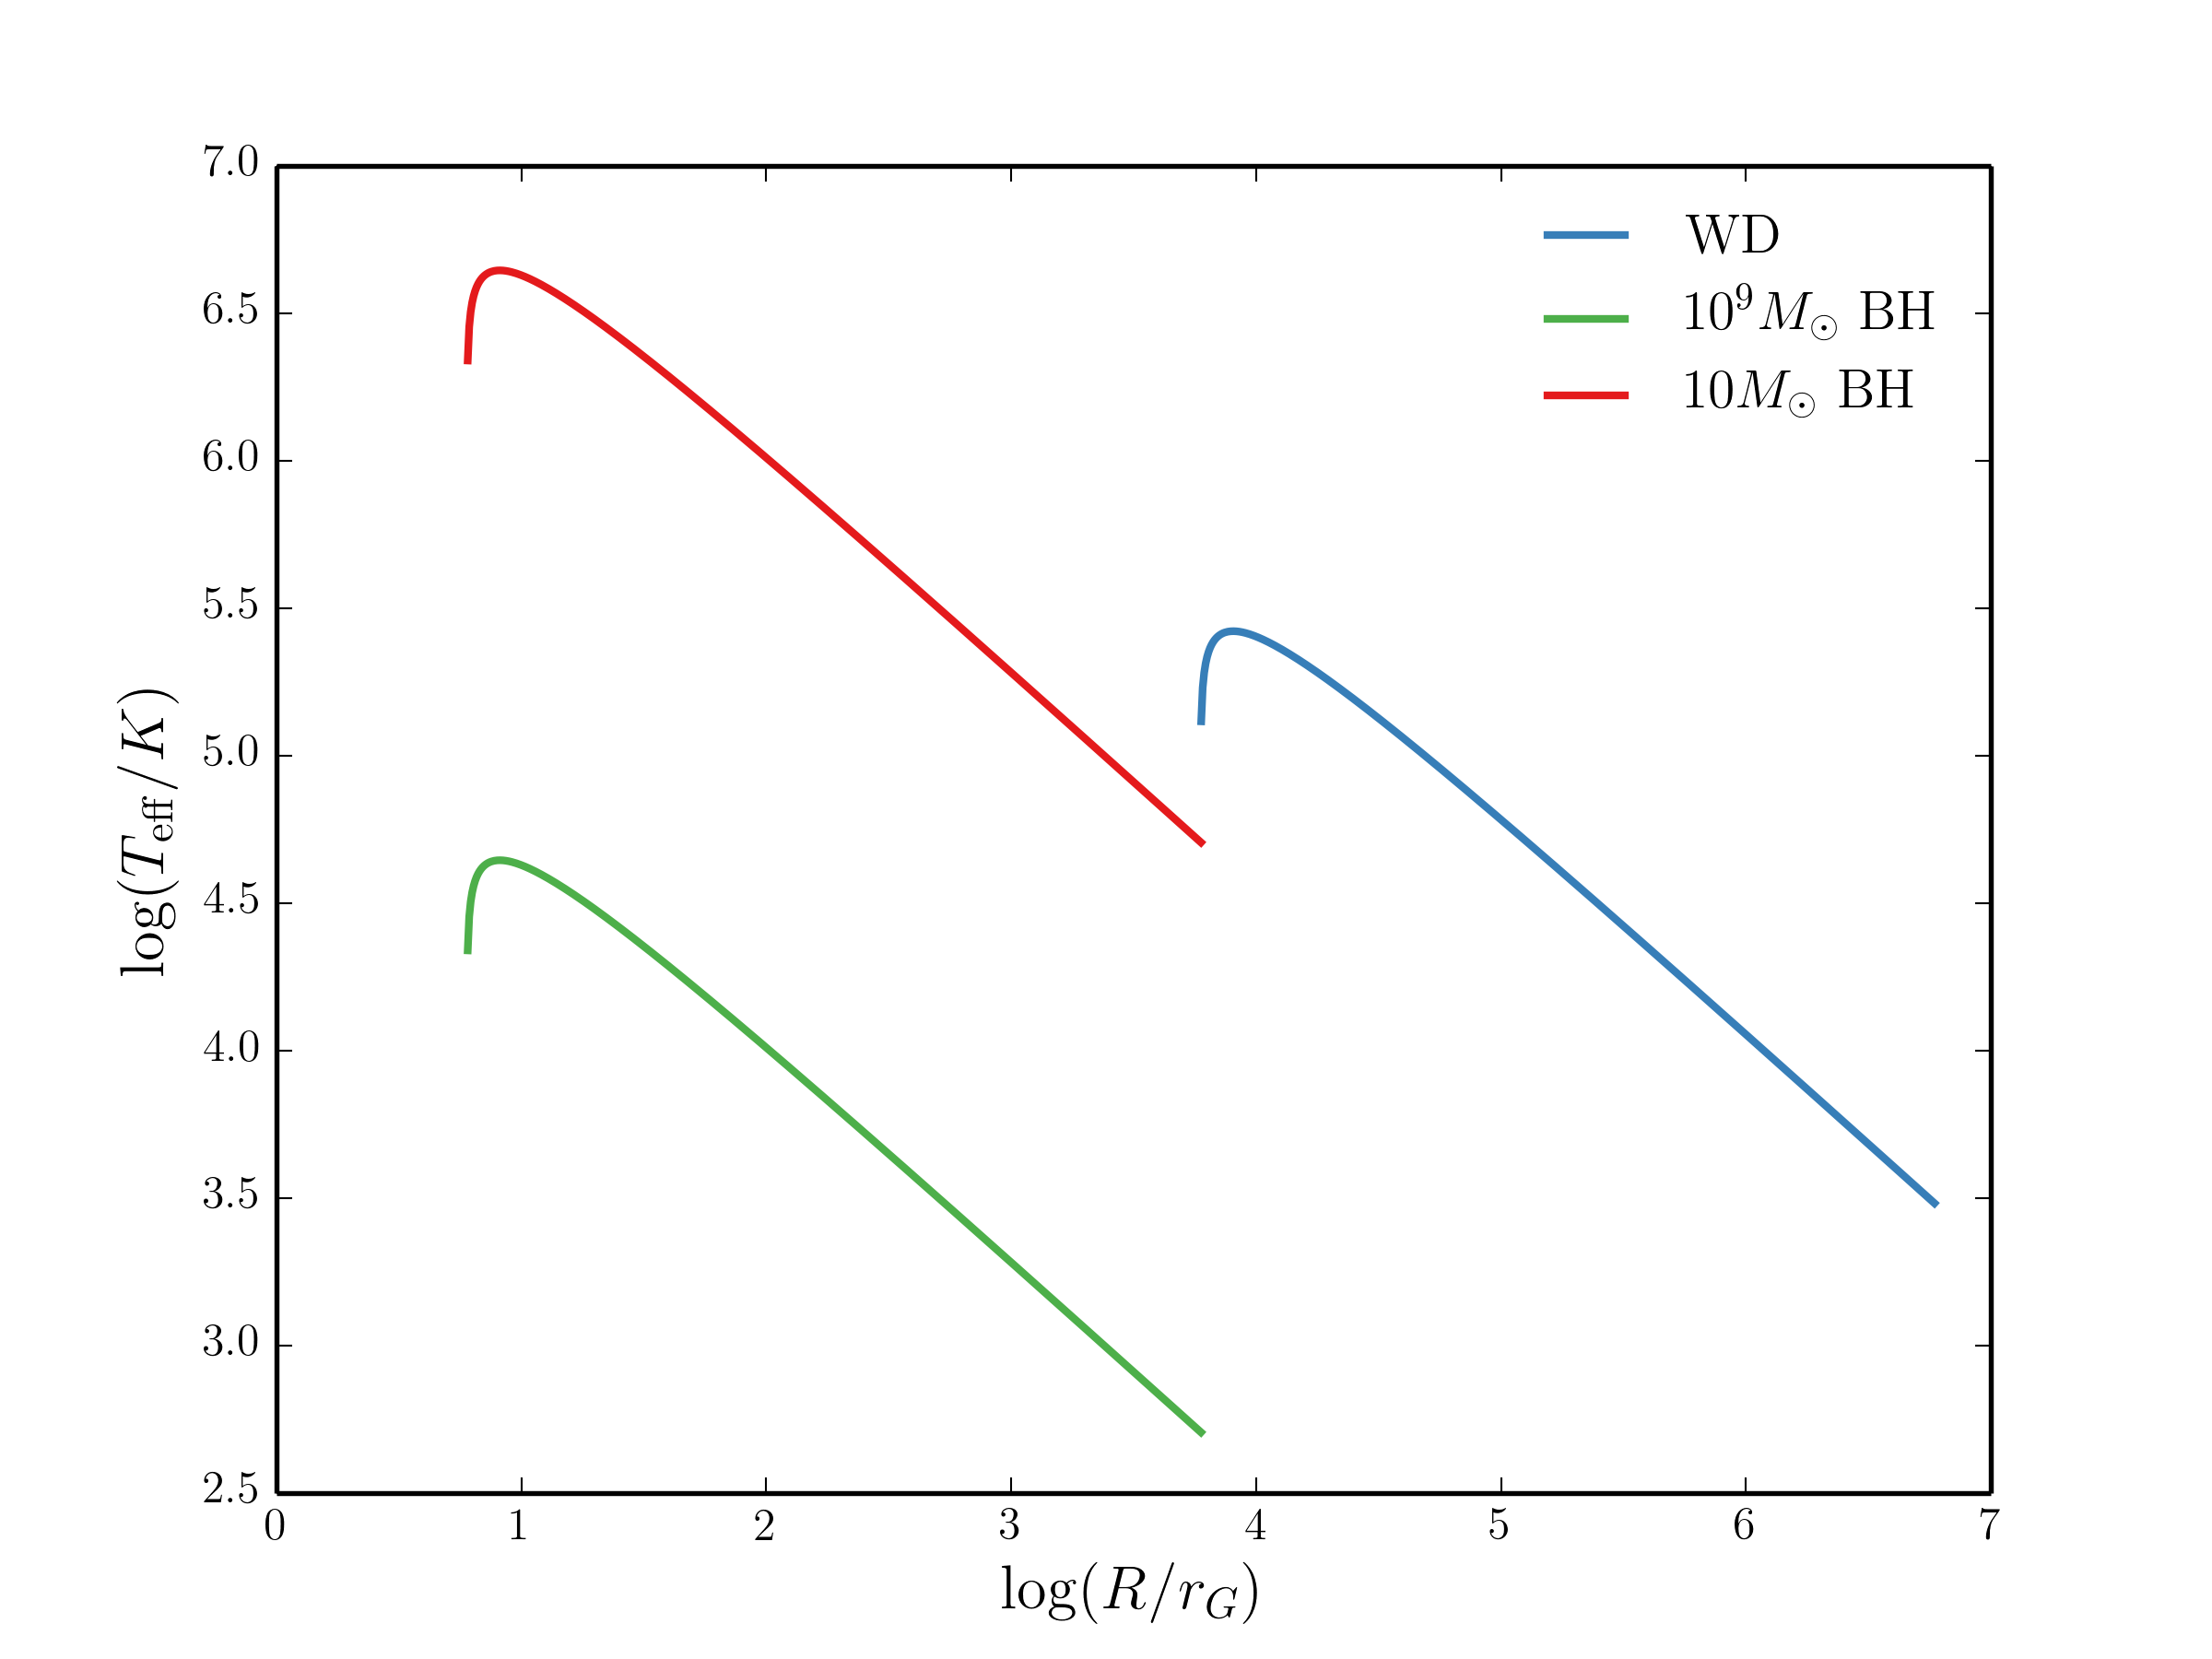
\includegraphics[width=1.0\textwidth]{figures/01-intro/disk_t.png}
\caption
[The temperature profile of an accretion disc for three different classes
of compact object.]
{
The temperature profile of an accretion disc for three different classes
of compact object.
} 
\label{fig:disk_t}
\end{figure}

\subsection{Boundary layers, black hole spin and the ISCO}

In equation~\ref{eq:ldisc} I showed that $L_{disc} = 1/2~L_{acc}$. 
One might then ask: where does the rest of the luminosity go?
The answer is dependent on the compact object in question. 
In an accreting WD, the rotating matter must eventually deposit itself 
on the surface of the WD. This is illustrated in figure~\ref{fig:omega},
which shows the angular velocity as a function of radius in a disc around
a compact object rotating with angular velocity $\Omega_*$. The boundary layer (BL)
is the region to the left of the dotted line, inside the maximum of $\Omega_K$, the Keplerian
angular velocity. The luminosity of the boundary layer is \citep{fkrbook}
\begin{equation}
L_{BL} = \frac{1}{2}\frac{GM \dot{M}}{R} \left[1 - \left(\frac{\Omega_*}{\Omega_K(R_*)}\right)\right]^2,
\end{equation}
where $\Omega_K(R_*)$ is the Keplerian angular velocity at $R_*$, assuming the thickness
of the BL is small. When $\Omega_K(R_*) \gg {\Omega_*}$, this reduces to 
$L_{BL} = 1/2~L_{acc} = L_{disc}$

In cataclysmic variables, 
BLs can be approximated with blackbodies and their temperatures estimated
indirectly via the \cite{zanstra1929} method \cite[e.g.][]{hoare1991,hoaredrew1993}.
Hopwever, they likely exhibit a variety of atomic features \citep{suleimanov2014}.
Extreme-UV (EUV) datasets have confirmed the existence of boundary layer emission
in non-magnetic CVs \citep{mauche1996}, although these observations
are limited in number.

\begin{figure}
\centering
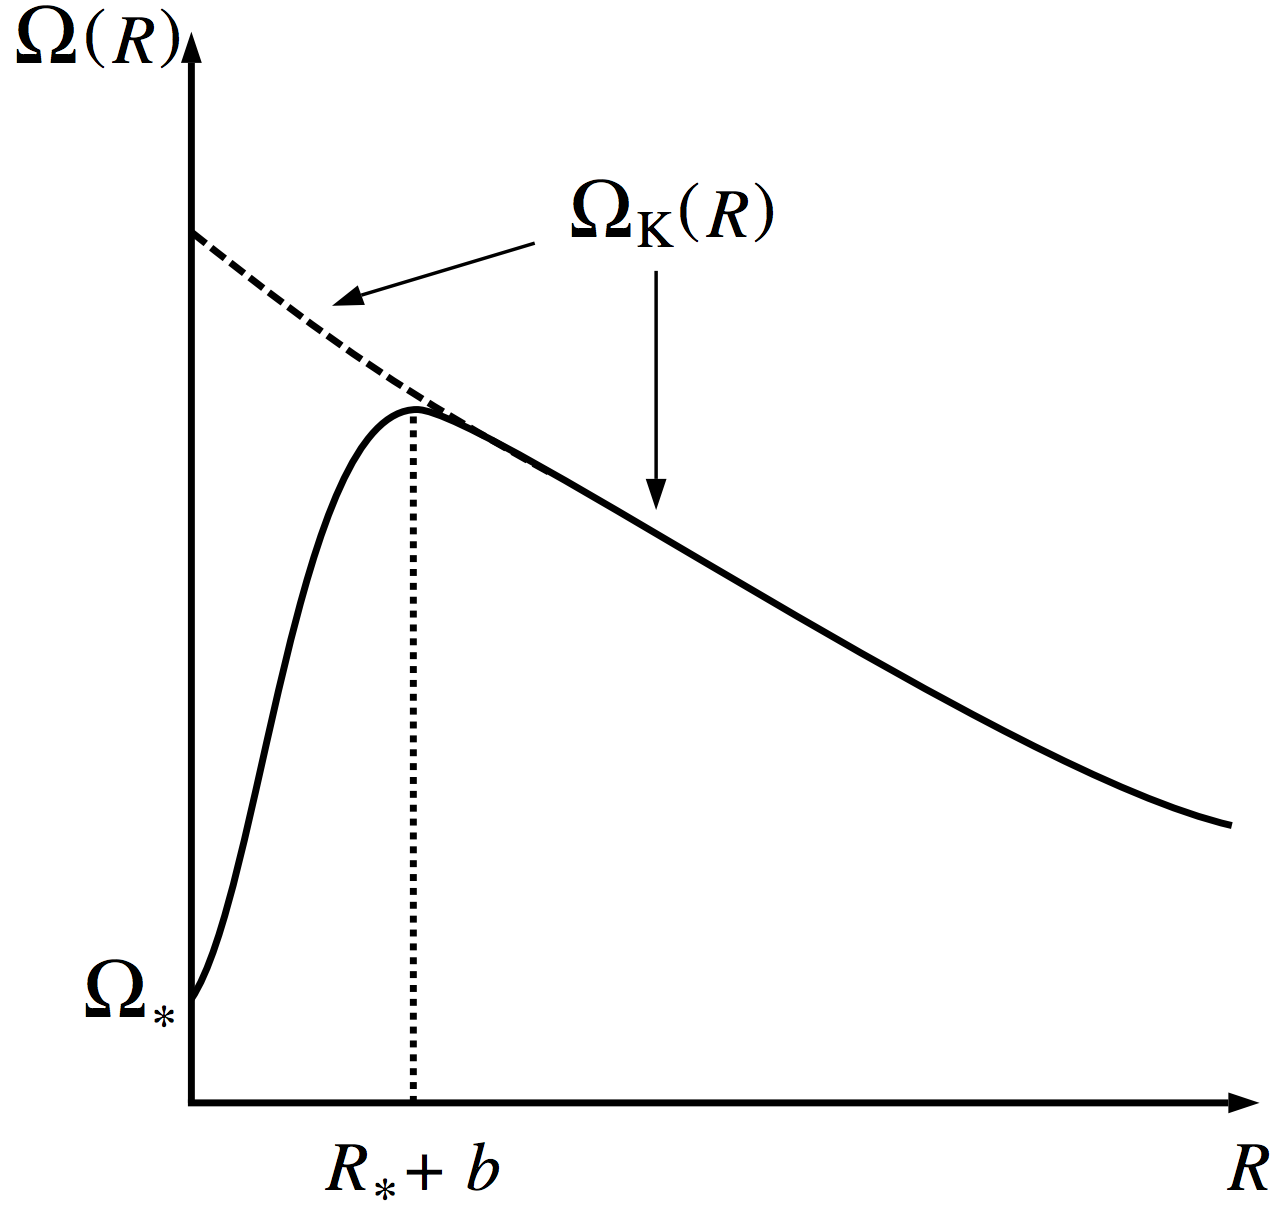
\includegraphics[width=0.7\textwidth]{figures/01-intro/omega.png}
\caption
[Angular velocity as a function of radius in an accretion disc around a rotating
compact object.]
{
{\sl Credit: Frank et al. 2002}.
Angular velocity as a function of radius in an accretion disc around a rotating
compact object with angular velocity $\Omega_*$. $\Omega_K$ is the Keplerian 
angular velocity. This graph
also helps explain why there is a turnover in the temperature-radius relation,
as $D(R)$ is proportional to the square of the {\em derivative} of this quantity.
} 
\label{fig:omega}
\end{figure}

Clearly, in BH systems a boundary layer cannot exist in the same way,
due to the lack of a physical surface. Instead, the energy must either go into
growing the BH, contributing to its angular momentum or being
channeled into a jet or other radiative source (see section~\ref{sec:disc-jet}).
The question of what happens at the inner disc edge
is complicated further by the fact that the disc cannot extend to the 
event horizon of the BH. Instead, there is an `innermost stable circular orbit' (ISCO)
beyond which the accreting matter will simply fall 
into the BH along nearly radial paths. The radius
of this orbit, $R_{ISCO}$, and the horizon radius, $R_H$,
is shown for different values of the BH spin parameter, $a_*$, 
in figure~\ref{fig:isco}, showing how matter can orbit closer to a prograde spinning BH. 
In estimating the luminosity of a Keplerian disc around a BH, 
one should really set $R_* = R_{ISCO}$ in equation~\ref{eq:eta}, giving us the interesting
result that rapidly spinning (Kerr) BHs are more radiatively efficient 
than Schwarzschild BHs.

\nocite{narayan2014, thorne1974}
\begin{figure}
\centering
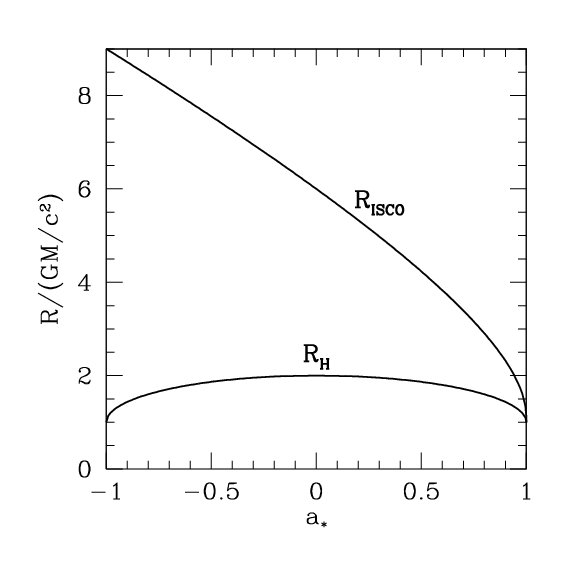
\includegraphics[width=0.7\textwidth]{figures/01-intro/isco.png}
\caption
[The radius of the ISCO, $R_{ISCO}$, and the horizon, $R_H$,
is as a function of the BH spin parameter, $a_*$.]
{
{\sl Credit: Narayan 2014.}
The radius of the ISCO, $R_{ISCO}$, and the horizon, $R_H$,
is as a function of the BH spin parameter, $a_*$. 
$a_*=0$ corresponds to a Schwarzschild BH, and $a_*=1$ and $a_*=-1$
to prograde and retrograde Kerr BHs respectively. Note that
this figure ignores the counteracting torque of photons swallowed by the BH,
which actually limits $a_*$ to a value of around $0.998$ (Thorne 1974).  
} 
\label{fig:isco}
\end{figure}


\subsection{The emergent spectrum}


\begin{figure}
\centering
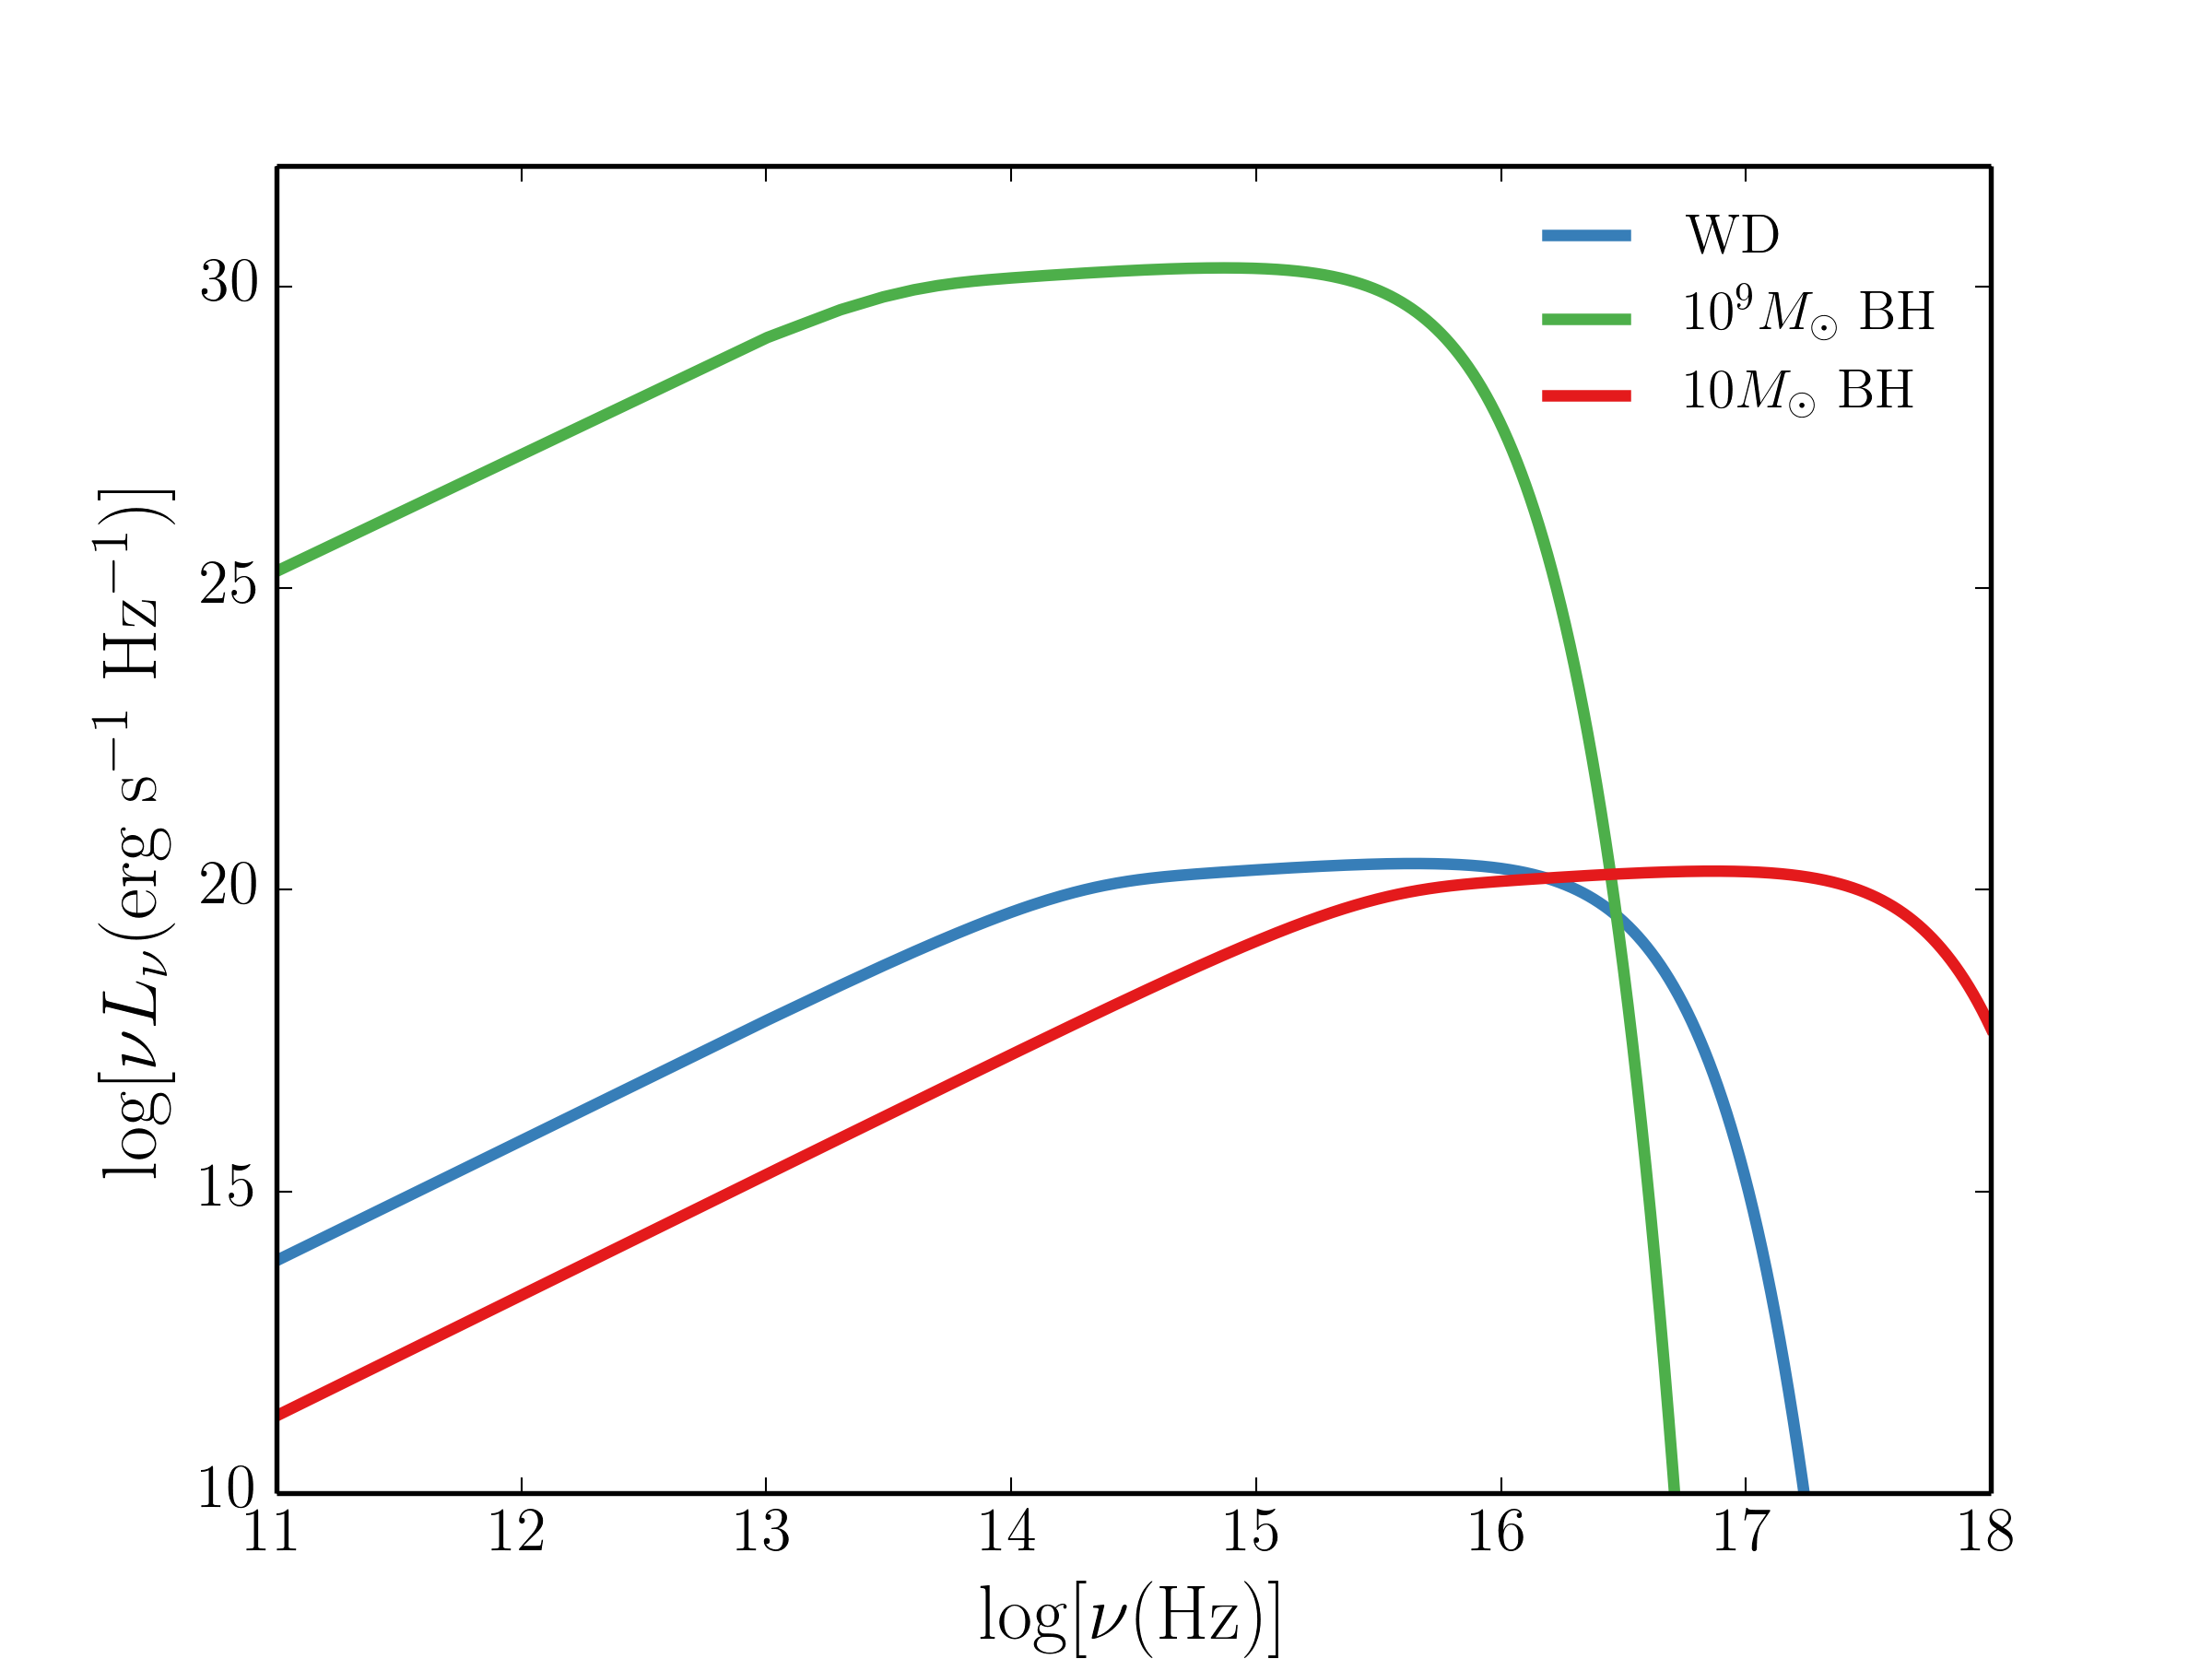
\includegraphics[width=0.8\textwidth]{figures/01-intro/disc_seds.png}
\caption
[Accretion disc SEDs for three different compact objects.]
{
Accretion disc SEDs for three different compact objects, corresponding roughly
to a quasar, an XRB and a CV. The SEDs are computed via an area-weighted sum
of blackbodies with effective temperatures governed by equation~\ref{disk_t_profile},
and the $\nu^{1/3}$ shape in the middle of the spectra can be seen.
} 
\label{fig:disc_seds}
\end{figure}

It is important to recognise that the steady-state disc treatment
{\sl does not specify the exact shape of the disc SED}. What it does do is 
say where energy is originally released. The simplest assumption is
that each annulus emits as a blackbody with temperature 
$T_{eff} (R)$, and the specific intensity through the emitting surface
thus follows the Planck Law:
\begin{equation}
B_\nu (T) = \frac{2 h \nu^3}{c^2} \frac{1}{\exp(h\nu / kT) - 1}
\label{eq:planck}
\end{equation}
Under this assumption it is possible to show that at intermediate frequencies, 
where $kT(R_{max}) \ll h \nu \ll kT_*$,
then the spectrum appears as a `stretched blackbody' with the form 
\begin{equation}
F_{\nu} \propto \nu^{1/3}.
\end{equation}
Figure~\ref{fig:disc_seds} shows the blackbody SEDs expected for the same 
objects as figure~\ref{fig:disk_t}, in
which the $\nu^{1/3}$ portion can be clearly seen.
A disc atmosphere model with frequency-dependent opacity creates a somewhat 
different (and more realistic) spectrum. 
Figure~\ref{fig:bb_v_sa} shows a comparison between a stellar atmosphere model and
blackbody model for $T_{eff}=50,000$K, showing how an annulus at that temperature
can have a significantly different spectral shape when one includes frequency-dependent opacities
in the atmosphere. It is of course possible that {\em neither} blackbody or disc atmosphere
treatments are realistic. I shall therefore devote a little time to discussing
the observational arguments for accretion discs and reviewing
the different classes of accreting objects.

\begin{figure}
\centering
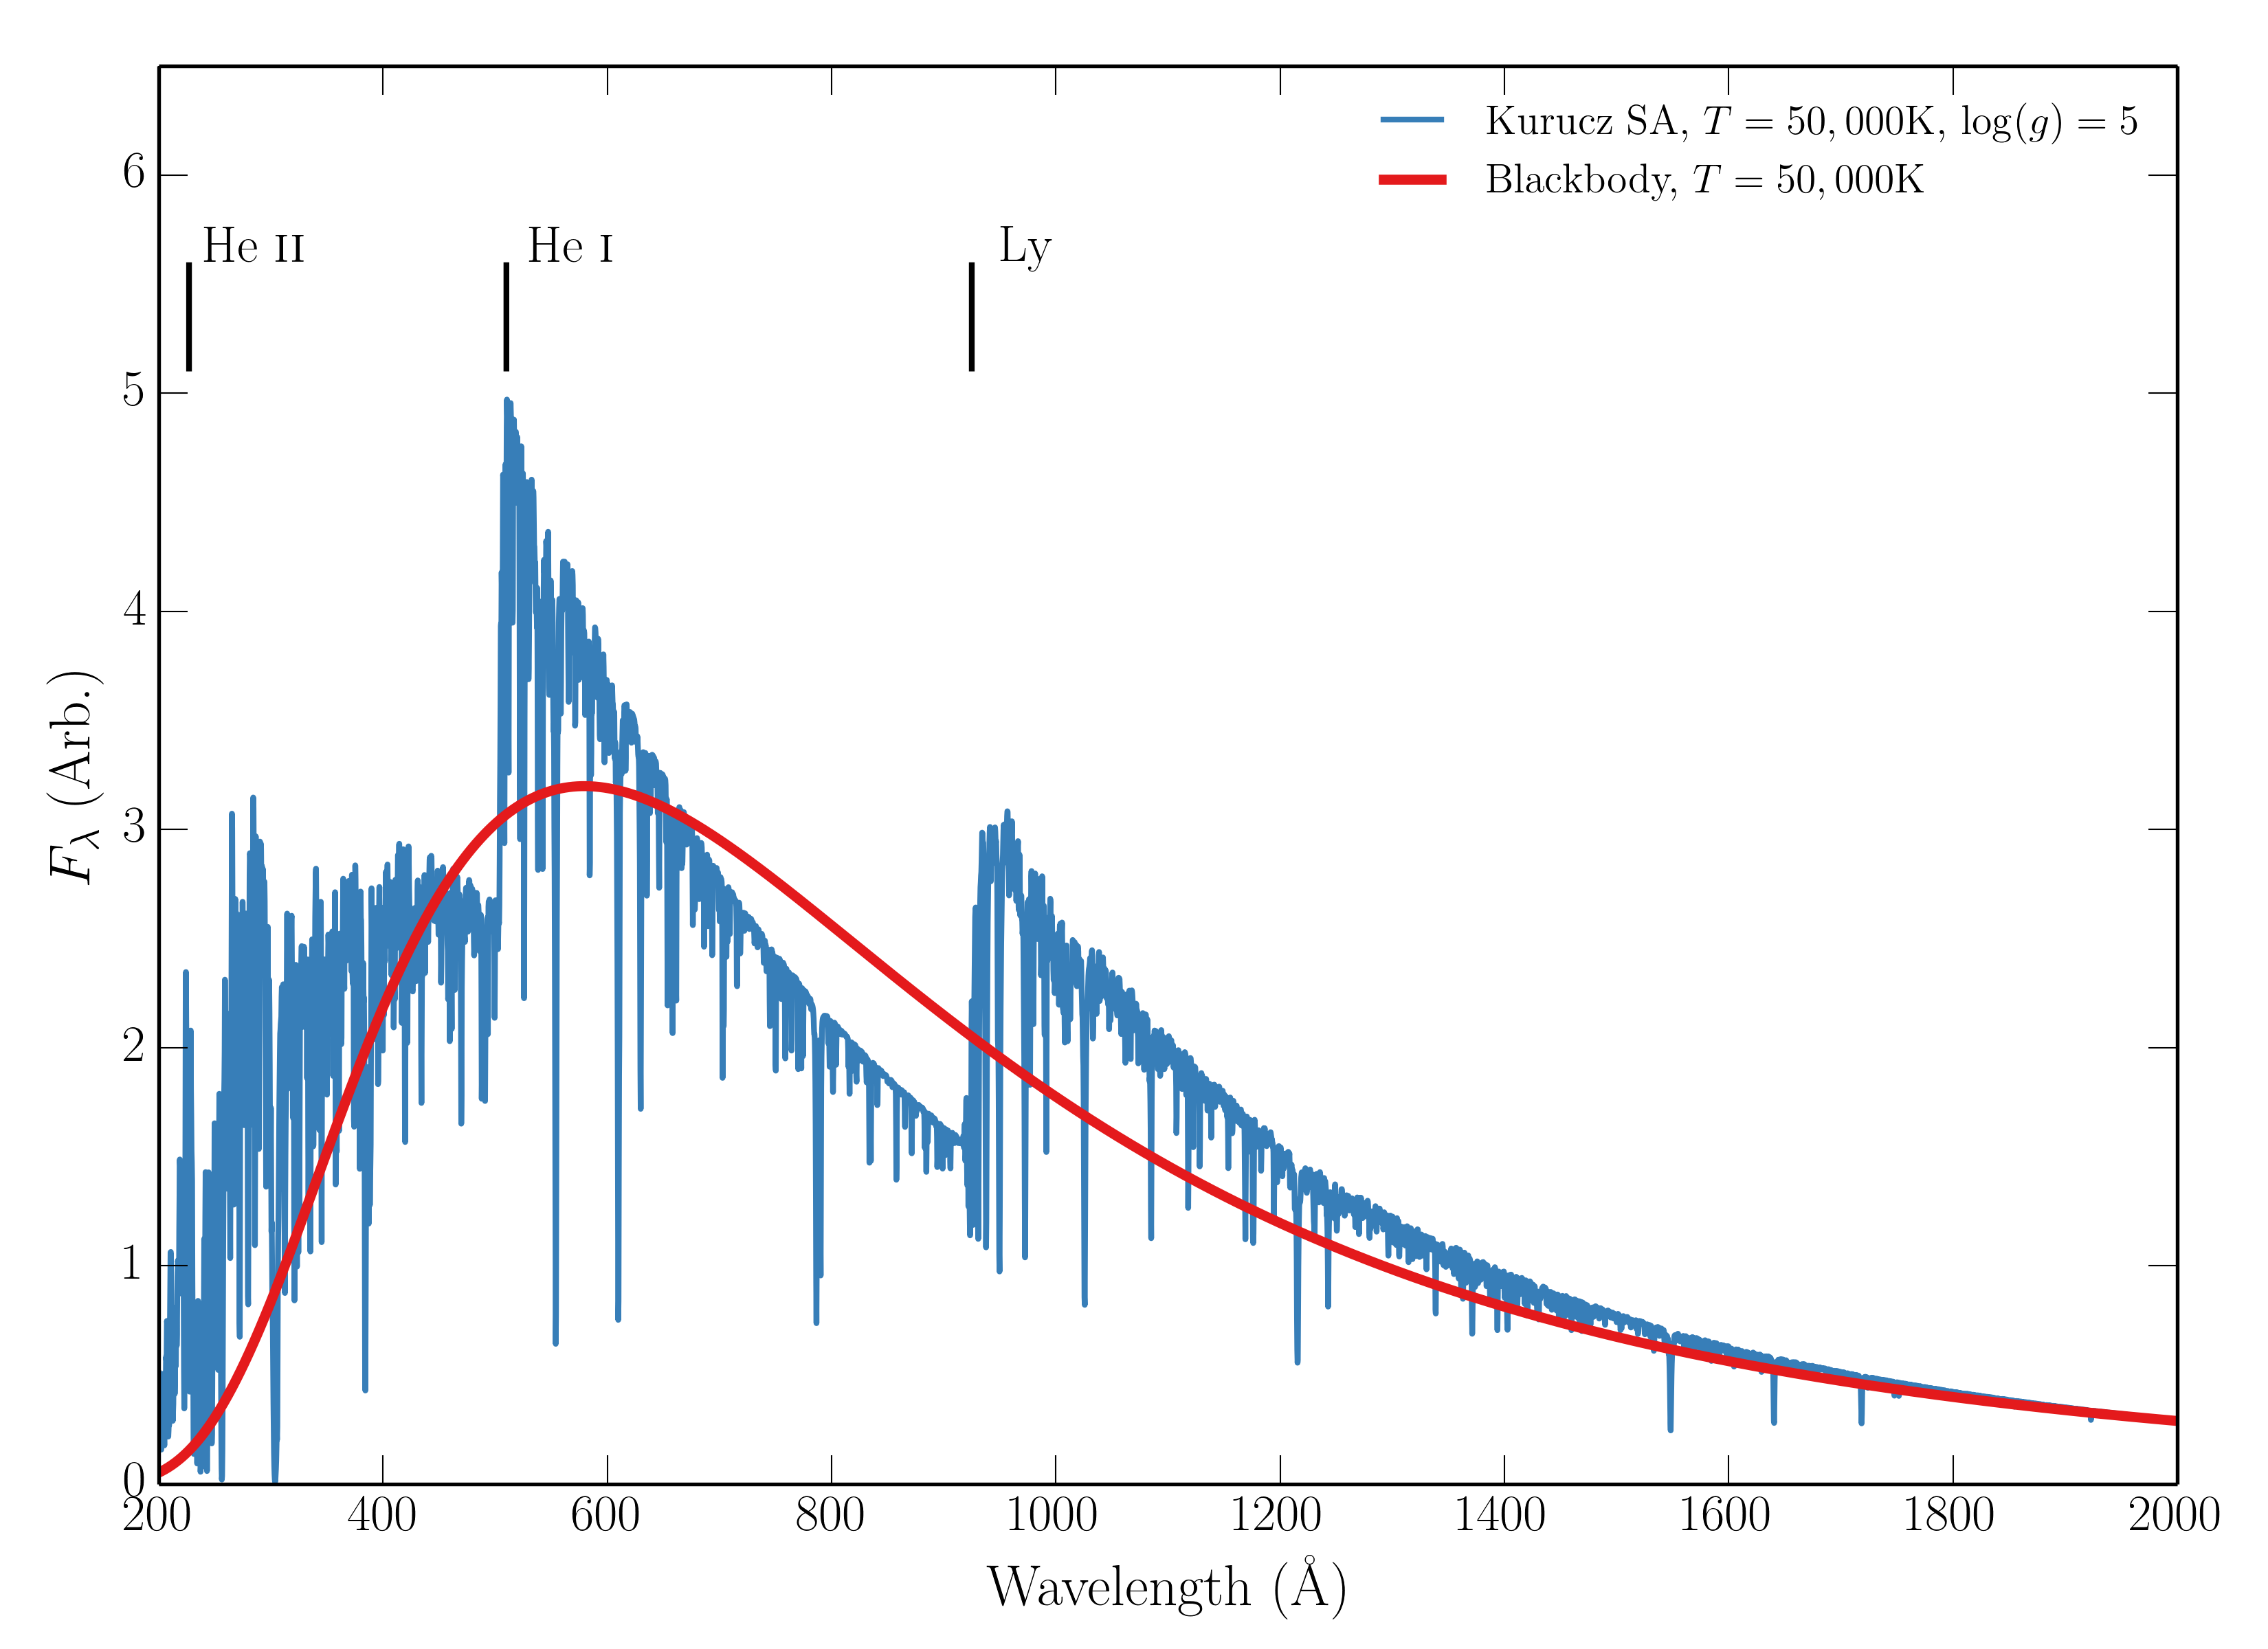
\includegraphics[width=0.8\textwidth]{figures/01-intro/bb_v_sa.png}
\caption
[A comparison between a Planck curve and Kurucz (1991) stellar atmosphere model.]
{
A comparison between a Planck curve and Kurucz (1991) stellar atmosphere model
at $T_{eff}=50,000$K and surface gravity of $\log(g)=5$. The major photoabsorption
edges are marked. Flux is reprocessed into different wavelengths by bound-free opacities,
and line blanketing also has a big effect on the spectrum. The Hydrogen and Helium lines
also experience significant pressure broadening.
} 
\label{fig:bb_v_sa}
\end{figure}


\section{Accreting Compact Binaries}

\begin{figure}
\centering
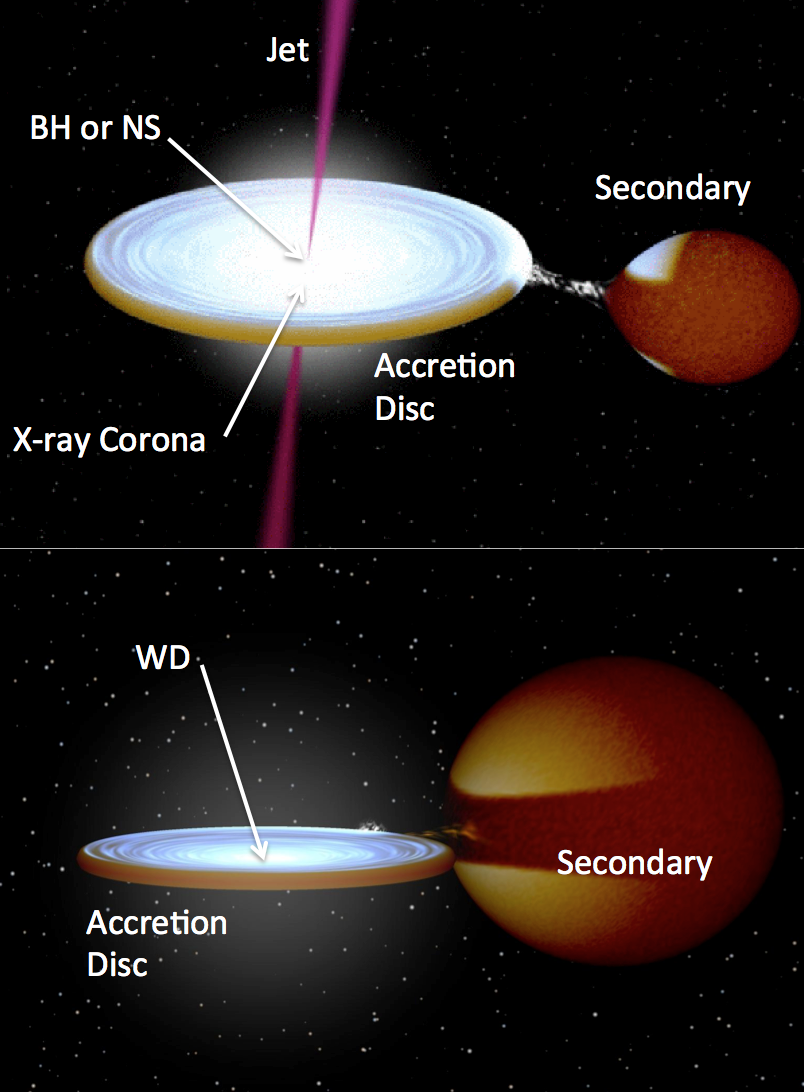
\includegraphics[width=1.0\textwidth]{figures/01-intro/cv_and_xrb.png}
\caption
[Artists impression of an LMXB and CV.]
{
{\sl Credit: Rob Hynes.} 
Artists impression of a low-mass X-ray binary (top) and
cataclysmic variable (bottom). The key components are marked,
and the clear similarity in overal structure is apparent.
} 
\label{fig:cv_and_xrb}
\end{figure}

Accreting compact binaries form many different classes, 
but are all characterised by matter streaming from a donor
onto a compact object. When the compact object is more massive 
than the donor then it is designated as the `primary', 
and the companion as the `secondary'. 
In high-mass X-ray binaries (HMXBs), the opposite is formally true.
There are only two ways by which matter can transfer 
from the secondary to the compact object. One is by Roche Lobe-overflow (RLOF),
whereby stellar evolution causes the donor star to fill its Roche Lobe, the surface
of equipotential around the star. The alternative is that the donor may expel
material via a disc or radiatively driven stellar wind, 
allowing some of it to flow onto the compact object. 
Although accretion from a wind or circumstellar disc is common in 
HMXBs \citep{bartlett2013}, here I will focus on 
RLOF as it is more common in the systems that possess high-state accretion discs
and associated outflows. Two examples of these are shown in figure~\ref{fig:cv_and_xrb}


\subsection{Roche Lobe-Overflow}

Let us consider a binary system, with masses $M_1$ and $M_2$, at positions
$\vec{r}_1$ and $\vec{r}_2$. The Roche potential, $\Phi_R$, in this system 
is then
\begin{equation}
\Phi_R = - \frac{GM_1}{| \vec{r} - \vec{r}_1 |} - 
\frac{GM_2}{| \vec{r} - \vec{r}_2 |} - 1/2 (\vec{\omega} \times
 \vec{r})^2,
\label{eq:roche}
\end{equation} 
where $\vec{\omega}$ is the angular velocity of the binary and is a vector normal to
the orbital plane. This potential is plotted in figure~\ref{fig:roche} for a mass ratio, 
$q = M_2 / M_1$ of 0.25.

\begin{figure}
\centering
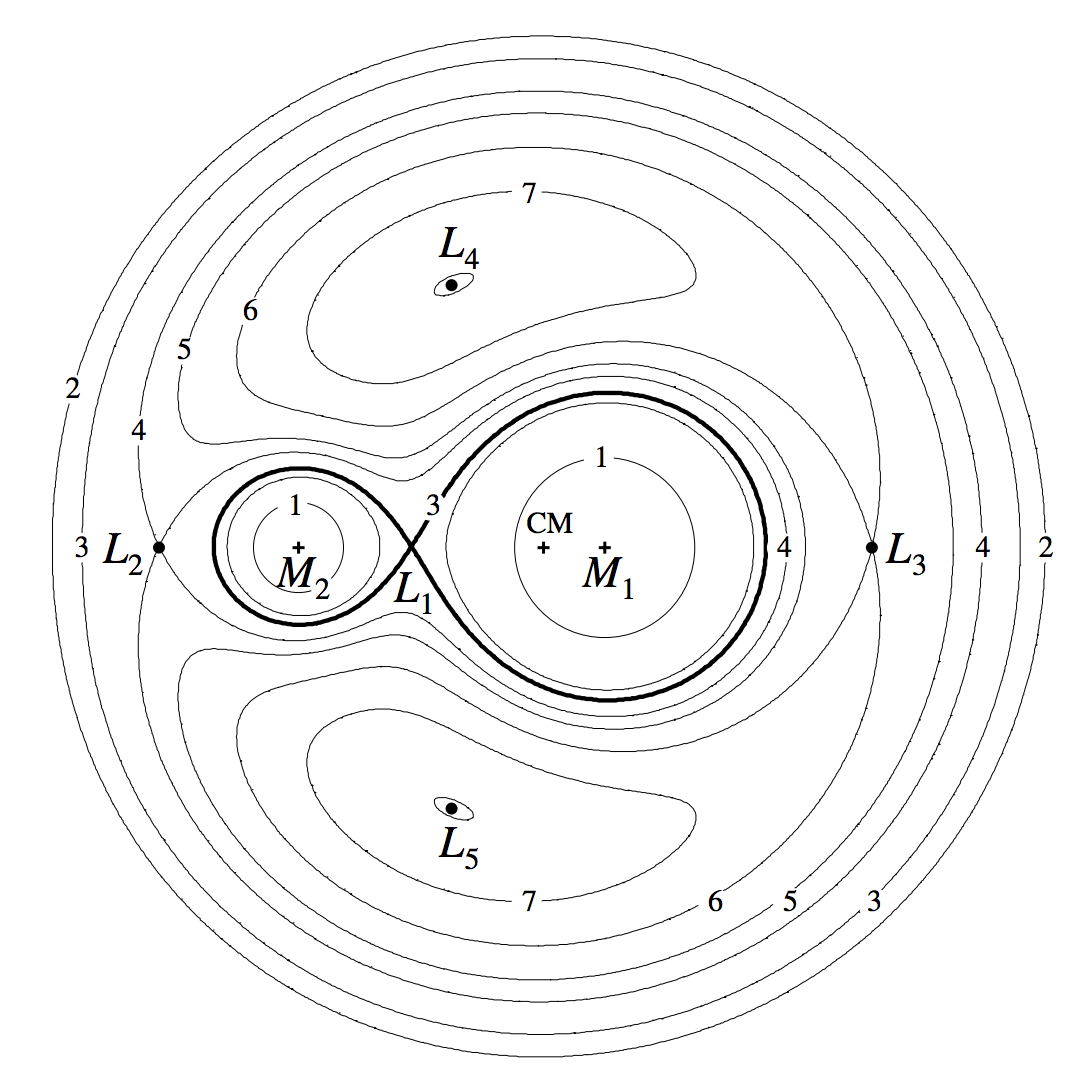
\includegraphics[width=0.7\textwidth]{figures/01-intro/roche_potential.png}
\caption
[The Roche potential in a binary system]
{
{\sl Credit: Frank et al. 2002.} 
The Roche potential in a binary system for $q = M_2 / M_1$ of 0.25.
The Lagrangian points are marked, as are the locations of the individual
and system centres of mass.
} 
\label{fig:roche}
\end{figure}

In the context of semi-detached binary systems, the most important region of the 
potential is the dumbbell shaped region enclosing the masses. Each of these
enclosed regions is known as the `Roche lobe' of the object and can be expressed 
approximately in terms of the mass ratio and separation of the system. A good approximation
for the size of the Roche lobe takes the form \citep{eggleton1983}
\begin{equation}
\frac{R_2}{a} = \frac{0.49 q^{2/3}}{0.6q^{2/3} + \ln(1+q^{1/3})}.
\label{eq:roche2}
\end{equation} 
Here $R_2$ is the radius of a sphere with the same volume as the Roche lobe for the
secondary star, which we can see depends only on $q$ and the orbital separation, 
$a$. If this secondary expands enough to fill its Roche lobe, then matter
will fall onto the other object. This process is known as Roche Lobe overflow (RLOF),
and is vitally important in astrophysics. Although caused by stellar evolution,
any accretion from RLOF will affect the mass ratio of the binary system 
and thus itself affects the evolution
of binary systems. This helps determine the orbital period
distribution of binaries \citep[e.g.][]{knigge2011_evo} 
as well as affecting the delay time distribution
of Type Ia Supernovae, for which CVs are one of the progenitor candidates 
\citep[e.g.][]{wang2012}.
It is also worth noting that the existence of gravitational waves has been 
required in models to explain the orbital period evolution of CVs since
the 1960s \citep{kraft1962}. 


\subsection{Cataclysmic Variables}

Cataclysmic variables (CVs) are systems in which a WD
accretes matter from a donor star via Roche-lobe overflow 
\citep[see the `CV bible', ][]{warnerbook}. 
CVs are not always dominated by their accretion luminosity; 
classical novae and super soft sources 
(SSS) emit mostly due to nuclear burning or detonation on the WD surface.
Accretion dominated CVs -- the focus here -- can be classified according to the 
magnetic field strength of the WD ($B_{WD} $) and photometric activity. 
Magnetic systems are classified as either `Polars' ($B_{WD} \gtrsim 10^7$~G)
or `Intermediate Polars' ($10^6 \lesssim B_{WD}  \gtrsim 10^7$~G);
in these systems the accretion flow inside the some critical radius 
(related to the Alfven radius)
is dominated by the WDs magnetic field \citep[e.g.][]{patterson1994}. 
In polars, this radius is large enough, due to the strong magnetic field,
that no disc forms at all \citep{liebert1985}.
When $B_{WD}  \lesssim 10^6$~G then the accreting material can fall
onto the WD via a disc, and the CV is classified as non-magnetic.
There are two main types of non-magnetic CVs; dwarf novae and nova-like
variables.

\subsubsection{Dwarf Novae and the Disc-instability Model}

Dwarf novae (DNe) are CVs that are characterised 
by repeated periods of quiescence and dramatic outburst. One of the 
most famous DNe is SS Cyg, whose light curve is shown in 
figure~\ref{fig:sscyg}. The repeated outbursts can be clearly seen, and
SS Cyg itself has been undergoing this behaviour for the full century 
for which it has been observed. A spectrum over the course of a 
typical outburst is shown in figure~\ref{fig:sscyg_spec}, 
and is characterised by the appearance of an optically thick
accretion disc continuum -- note the similarity to the 
stellar atmosphere disc spectrum computed in section~\ref{sec:alpha_disc},
and to the intermediate inclination nova-like variables discussed in the next
section.

The leading scnario for explaining DN outbursts, and in fact also the outbursts
in low mass X-ray binaries or `soft X-ray transients',
is the disc-instability model 
\citep[DIM; ][]{osaki1974,lasota2001}. 
In this model, a gradual increase in supply rate from the donor star 
(and hence surface density in the disc) 
causes the disc to heat up. Eventually, the disc hits a critical temperature,
around $7000$~K, and becomes ionized. Now the surface density in the disc
can increase significantly, and the disc becomes geometrically thin and
optically thick. Most importantly, it can undergo efficient radiative
cooling, and a significant increase in brightness is observed.

\begin{figure}
\centering
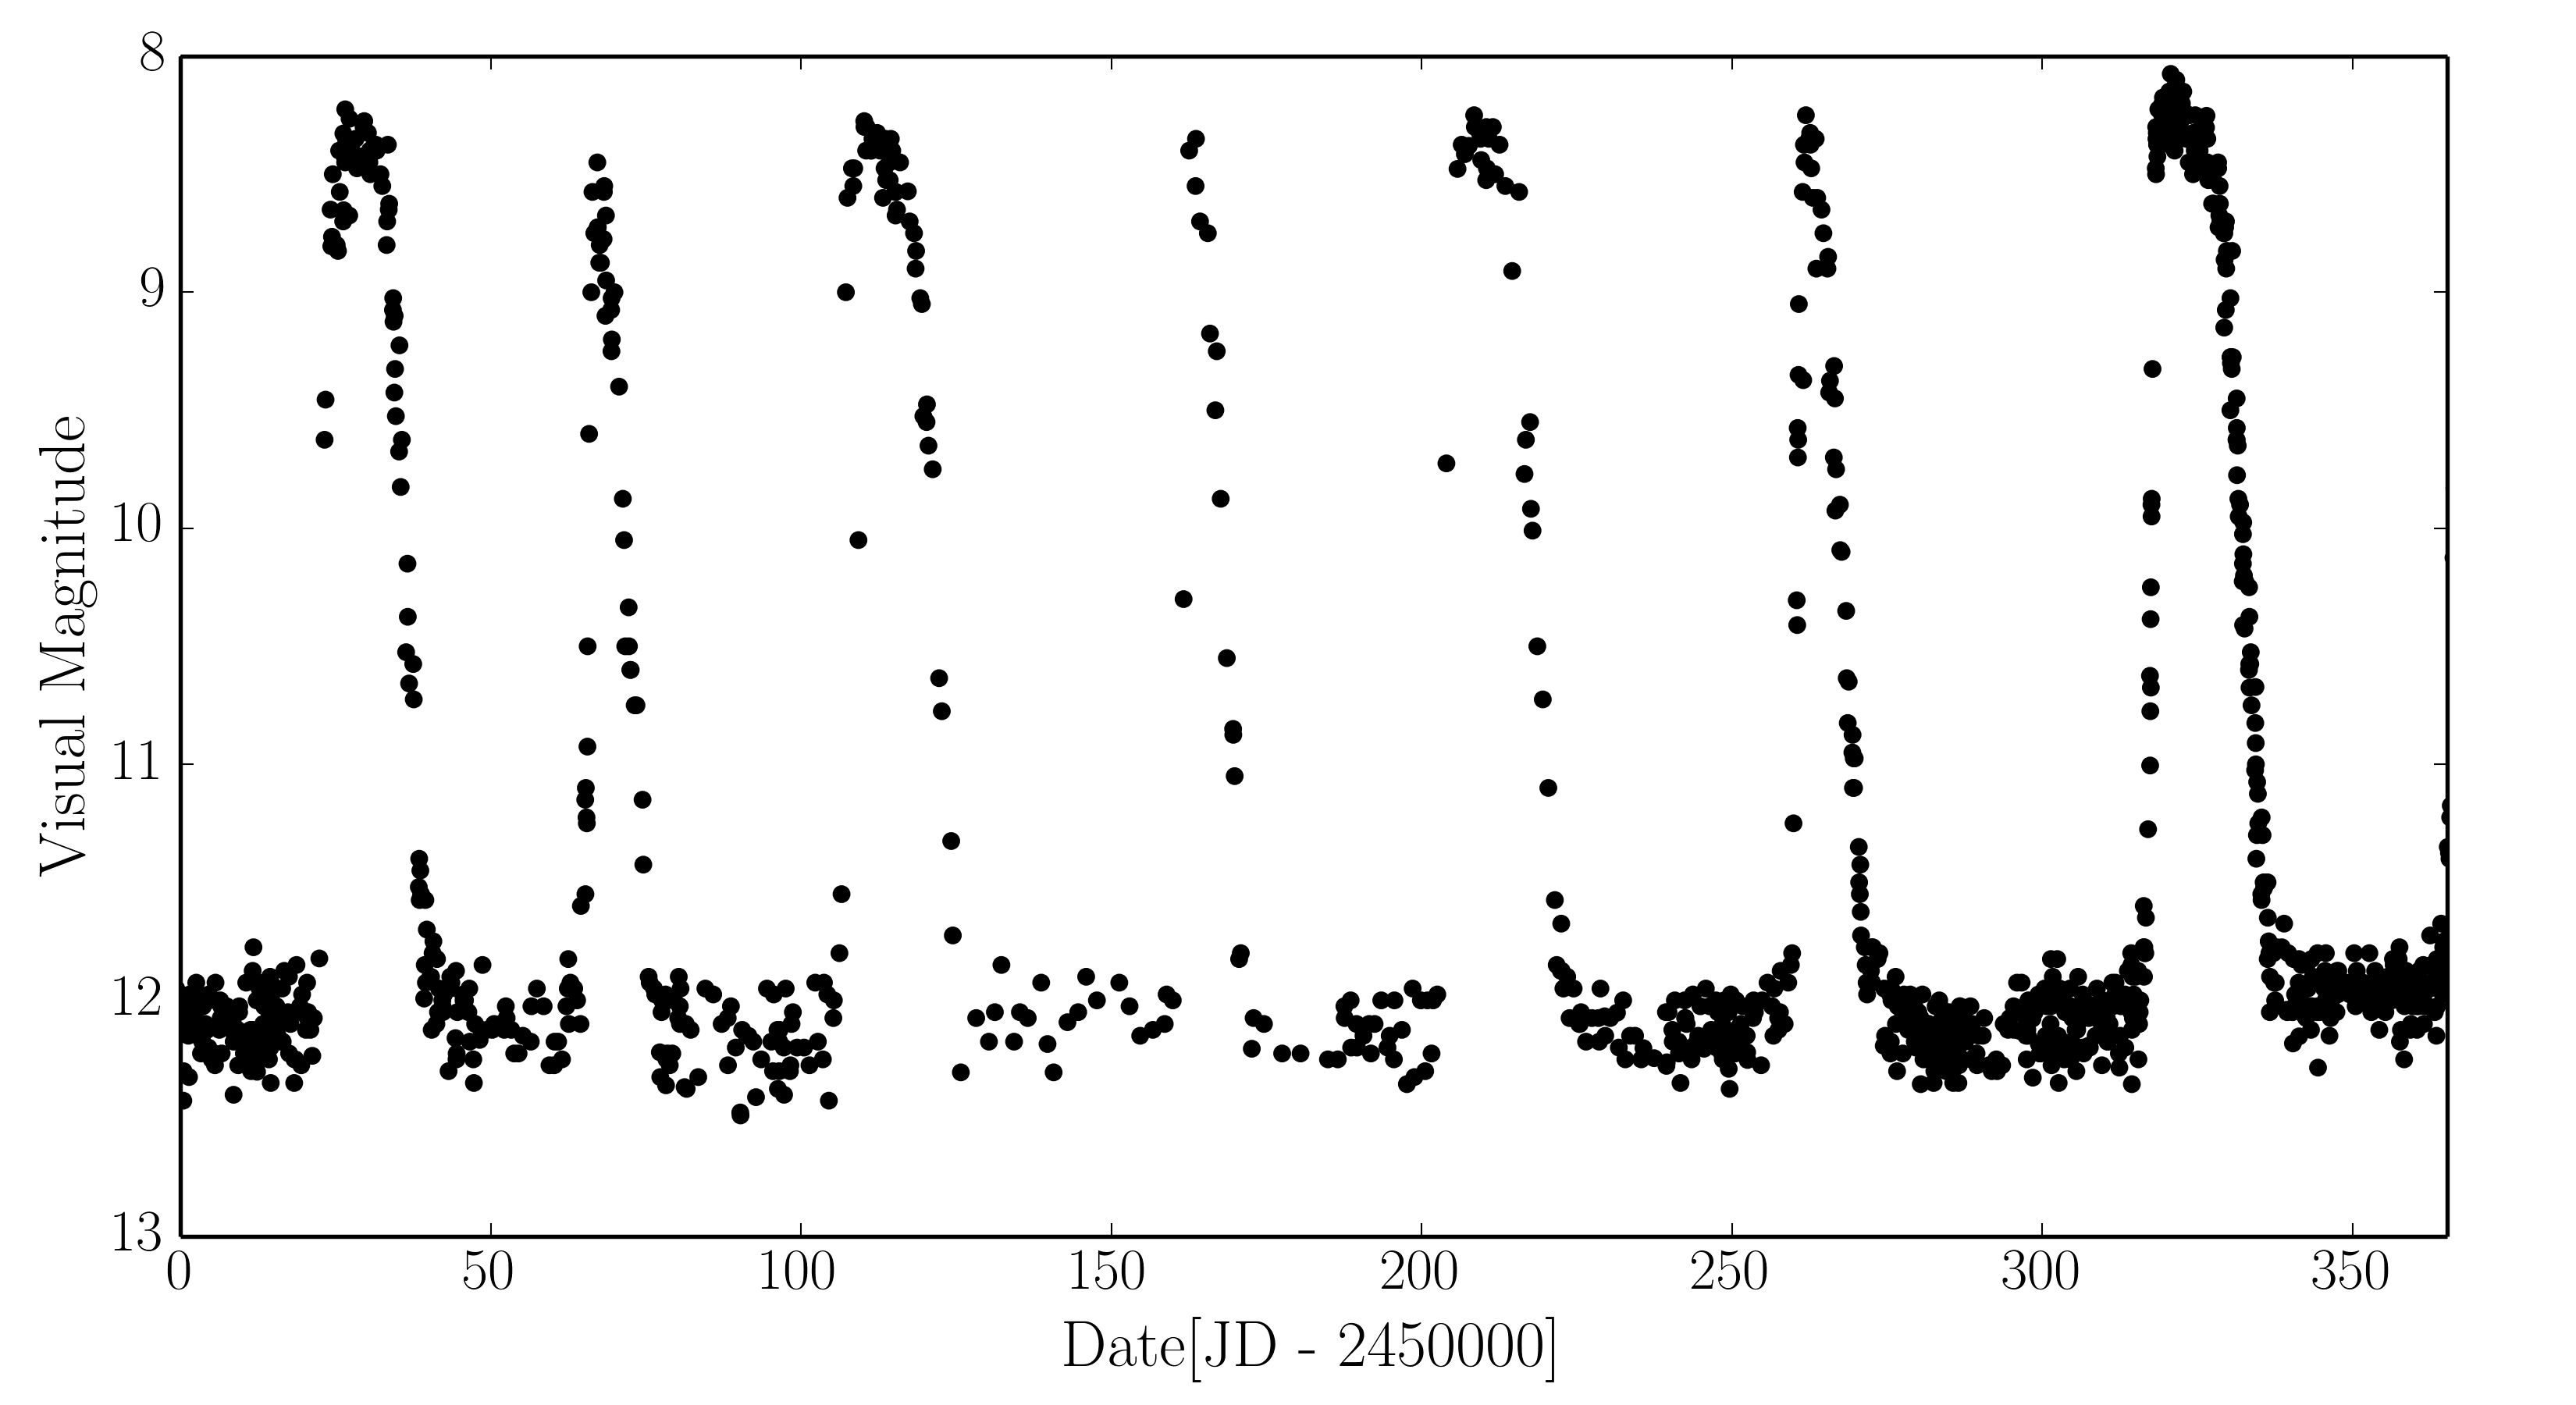
\includegraphics[width=1.0\textwidth]{figures/01-intro/lc_sscyg.png}
\caption
[A year in the life of SS Cyg.]
{
{\sl Data: AAVSO.} 
A year in the life of SS Cyg, showing the characteristic repeated
outbursts and periods of quiescence typical of a DN. SS Cyg has been
undergoing this activity since it was first observed in 1896.
} 
\label{fig:sscyg}
\end{figure}

\nocite{dhillon1996,hessman1984}
\begin{figure}
\centering
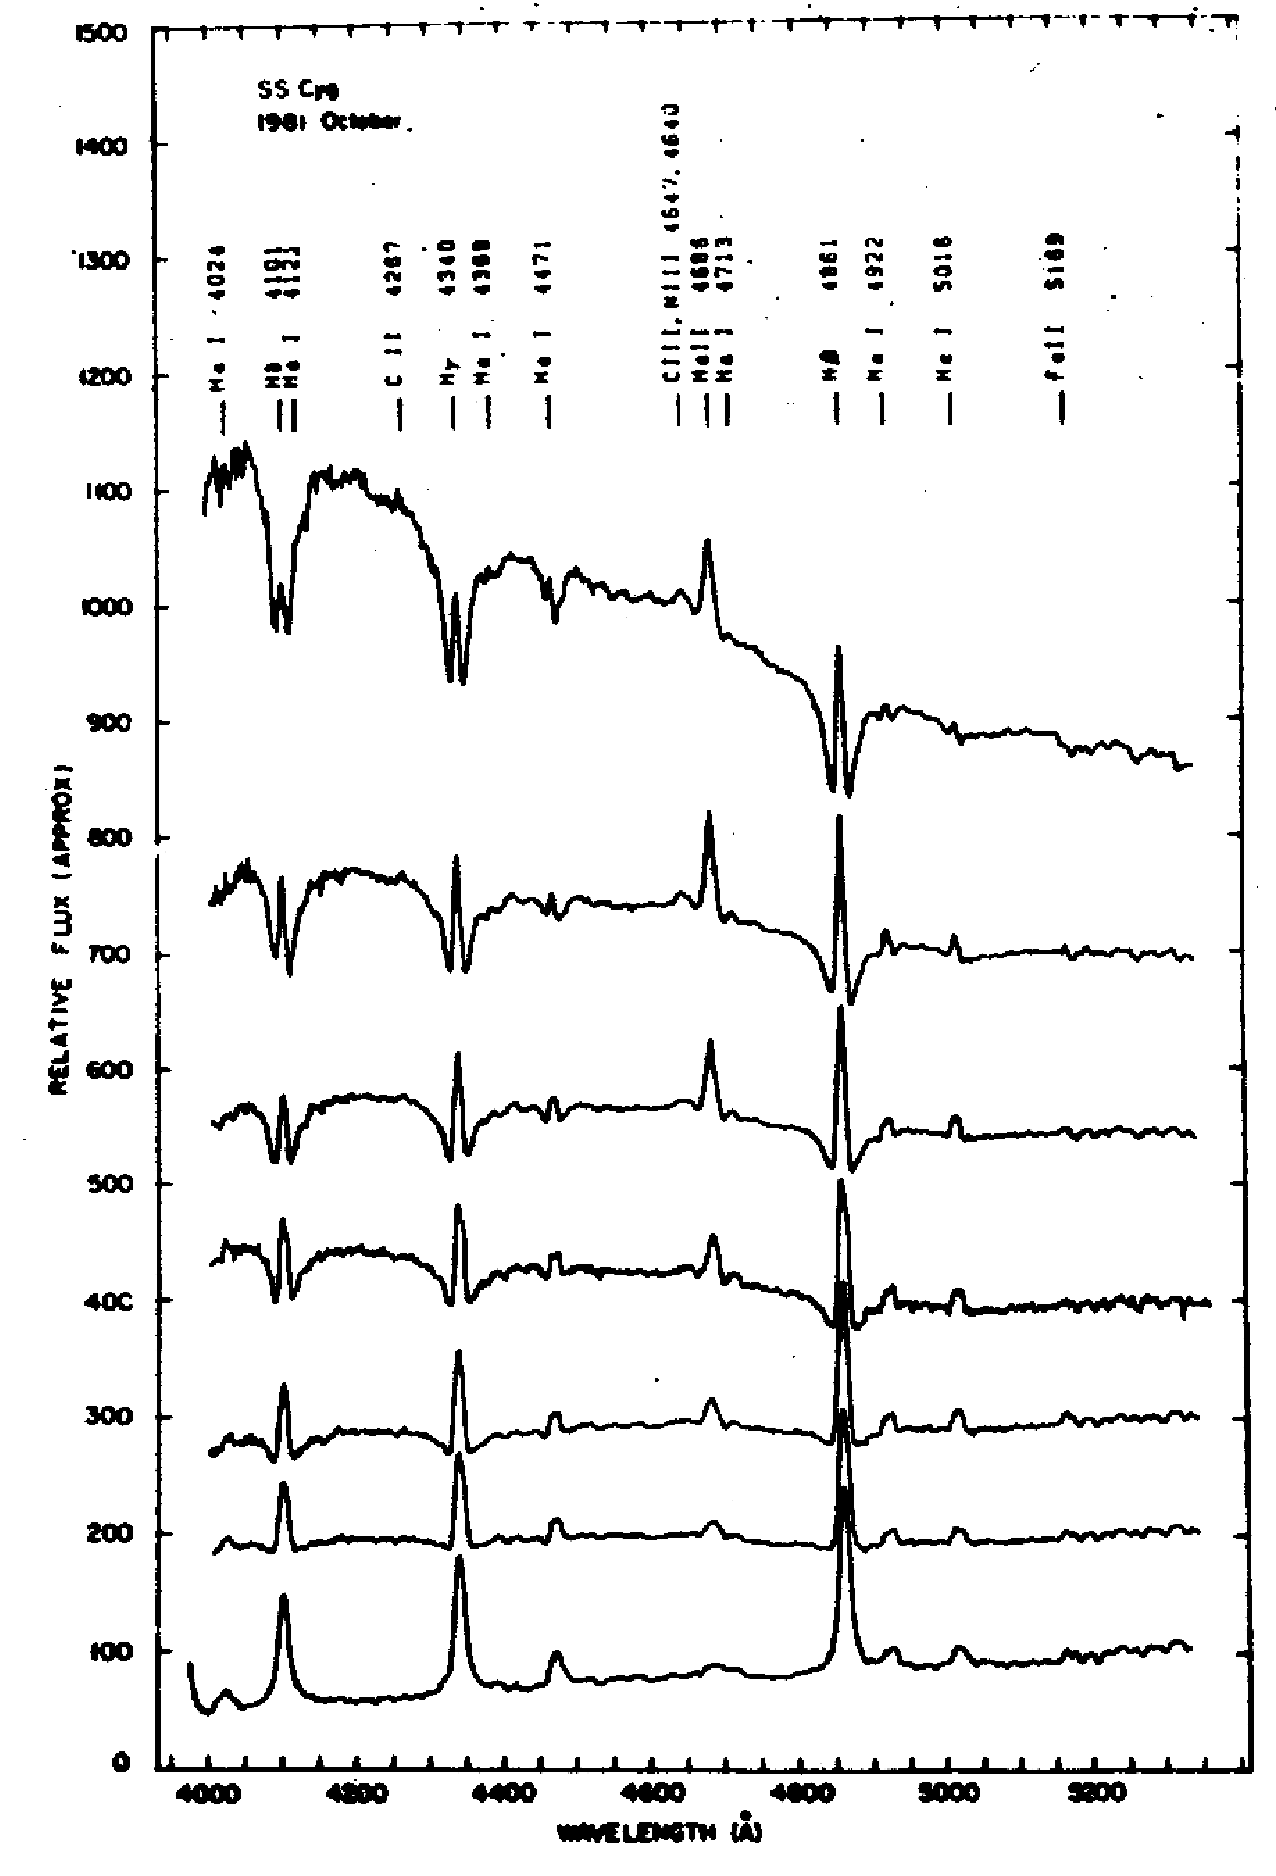
\includegraphics[width=1.0\textwidth]{figures/01-intro/sscyg_spec.png}
\caption
[Spectra of SS Cyg during an outburst cycle]
{
{\sl Credit: Hessman et al. 1984 / Dhillon et al. 1996.} 
Spectra of SS Cyg during an outburst cycle, showing the evolution from 
minimum to maximum light. The rise is characterised by the appearance of an
optically thick accretion disc spectrum. The flux scale is approximate.
} 
\label{fig:sscyg_spec}
\end{figure}

\subsubsection{Nova-like Variables}

\nocite{dhillon1996,hessman1984}
\begin{figure}
\centering
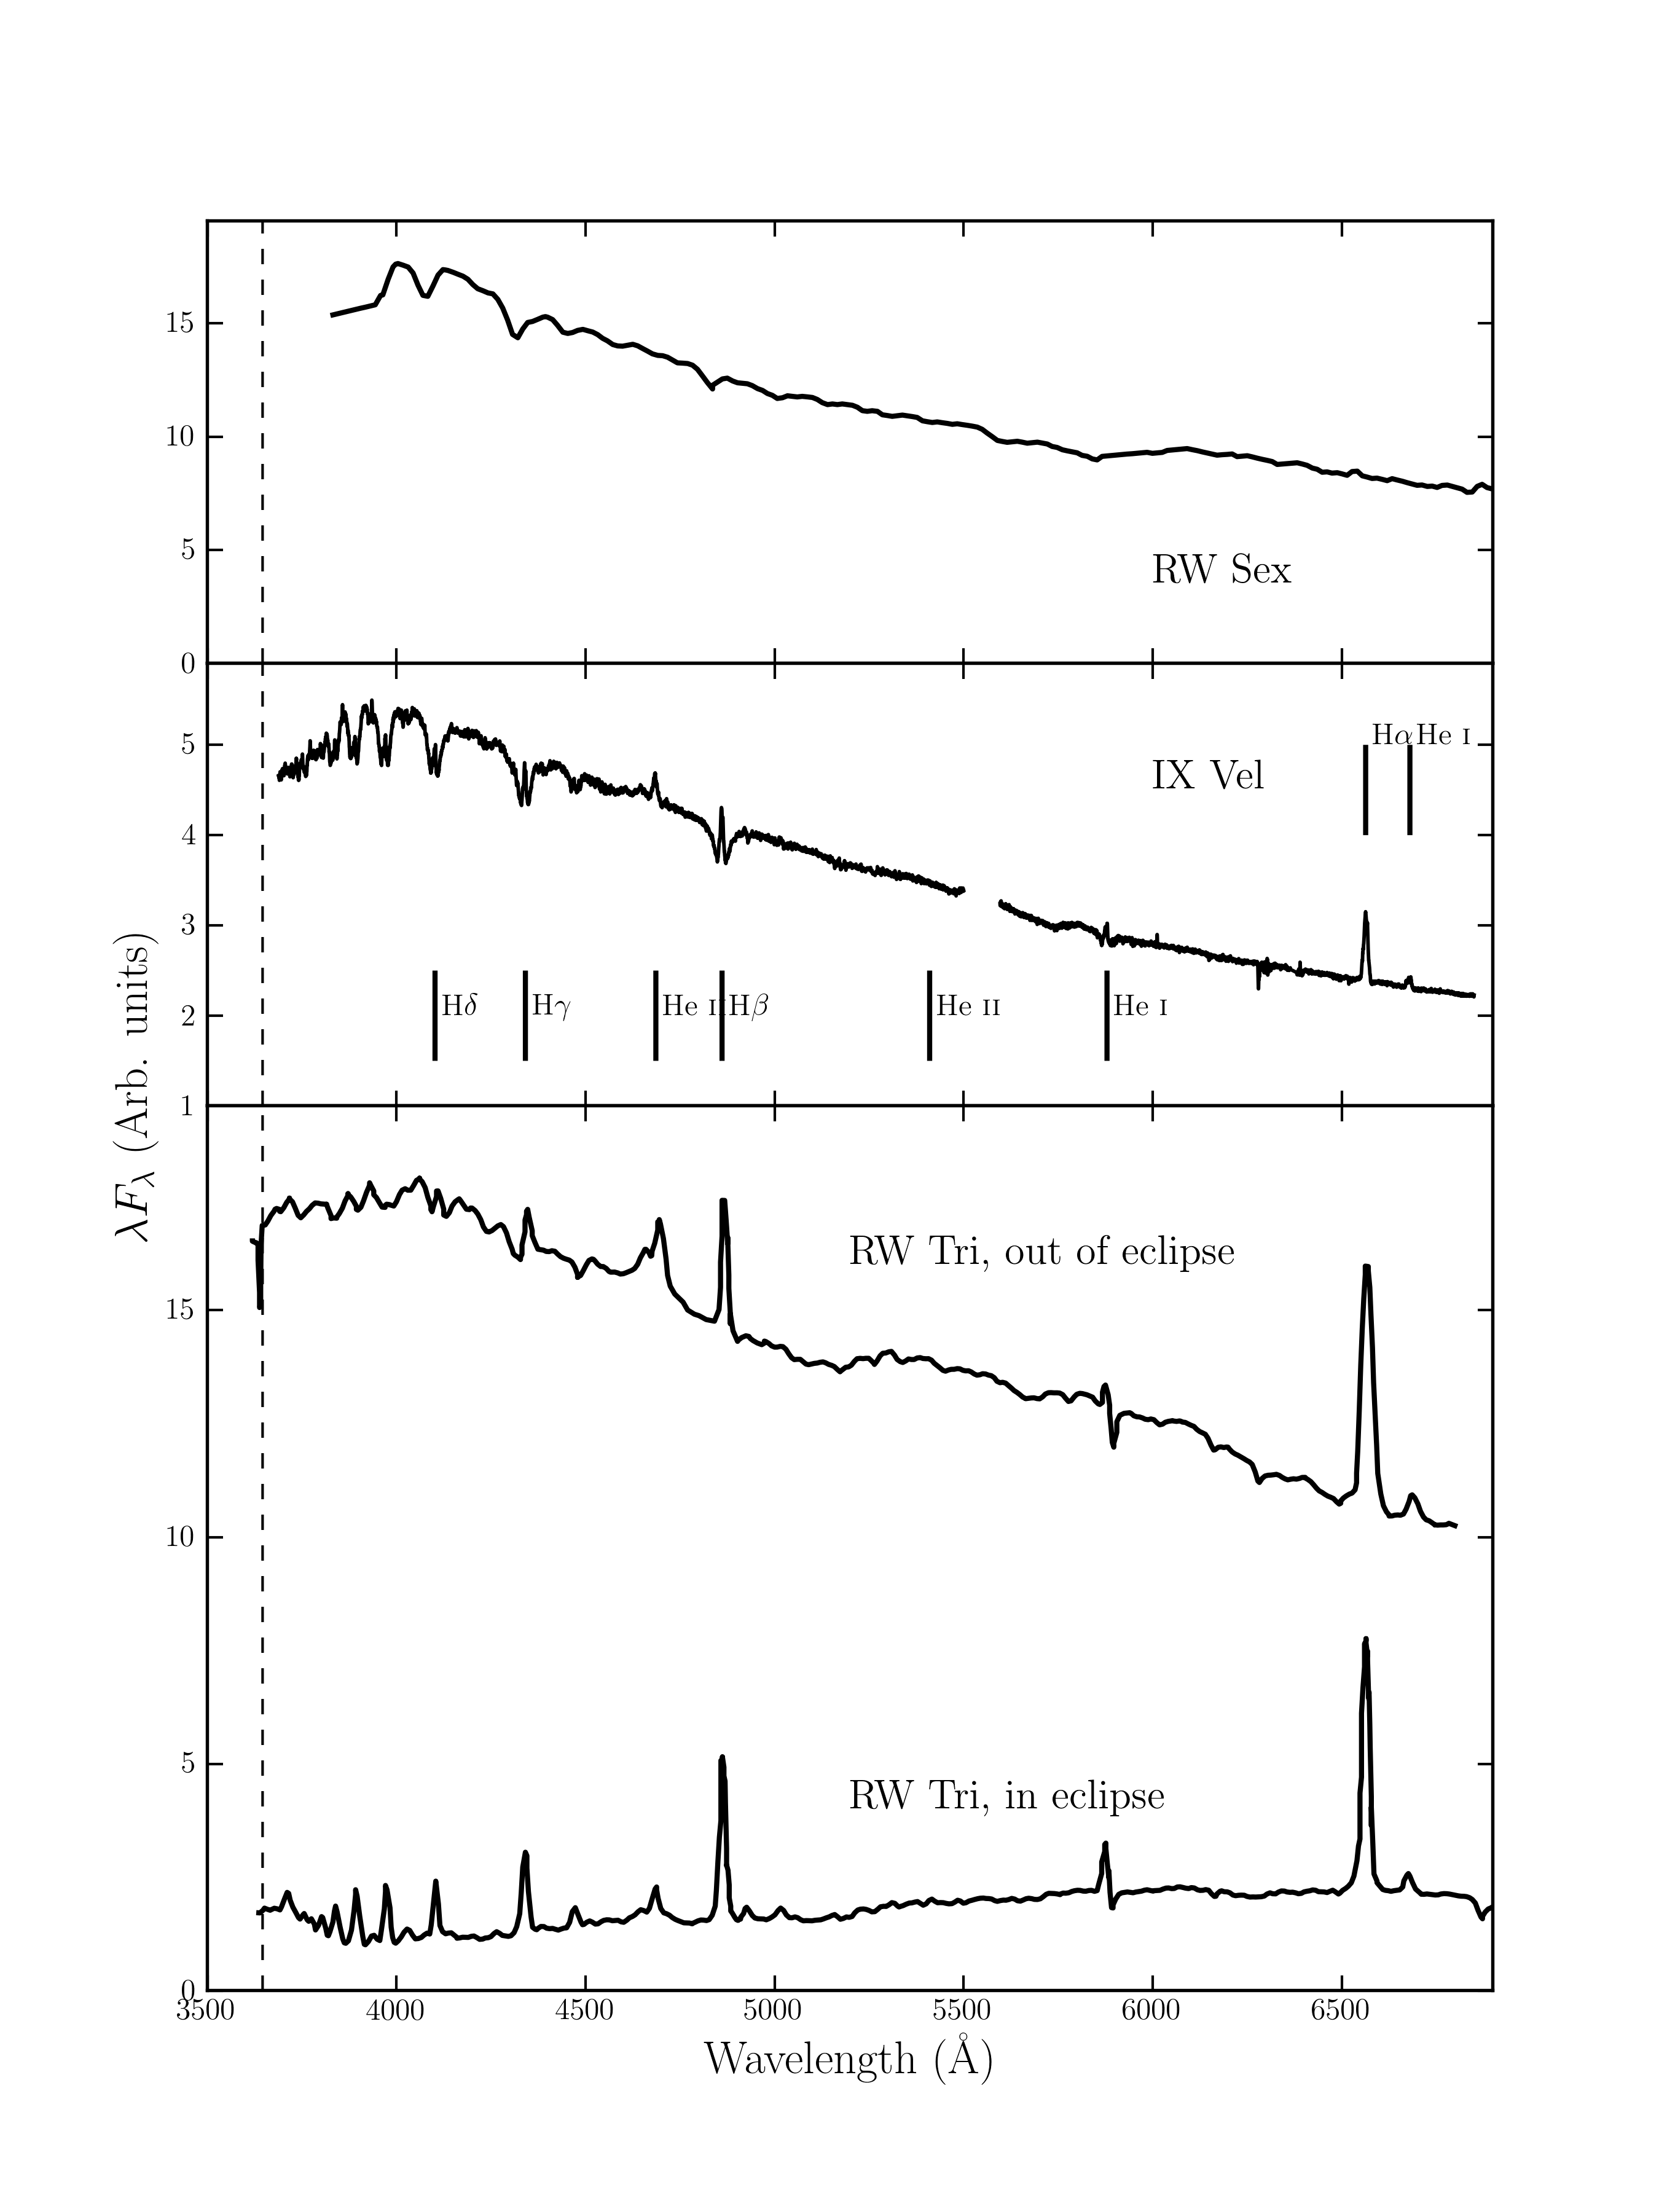
\includegraphics[width=1.0\textwidth, clip=true, trim= 0 0.6in 0 0.8in]{figures/01-intro/novalikes.png}
\caption
[Optical spectra of three nova-like variables.]
{
Optical spectra of three nova-like variables: 
RW Sex (top; Beuermann et al. 1992),
IX Vel (top middle; A. F. Pala \& B. T. Gaensicke, private communication) 
and RW Tri in and out of eclipse (bottom two panels; Groot et al. 2004).
The data for RW Sex and RW Tri were digitized from the respective publications,
and the IX Vel spectrum was obtained using the XSHOOTER spectrograph 
on the Very Large Telescope on 2014 October 10.
These systems have approximate inclinations of 
$30^\circ$, $60^\circ$ and $80^\circ$ respectively. 
The trend of increasing Balmer line emission with inclination can be seen.
In RW Tri strong single-peaked emission in the Balmer lines is seen even
in eclipse, indicating that the lines may be formed in a spatially
extensive disc wind, and there is even a suggestion 
of a (potentially wind-formed) recombination continuum in the eclipsed
spectrum. I have attempted to show each spectrum over a similar dynamic range.
} 
\label{fig:NL_spec}
\end{figure}

Nova-like variables (NLs) are similar to DNe,
except that the disc is always in a relatively 
high-accretion-rate state ($\dot{M} \sim 10^{-8}$~M$_{\odot}$~yr$^{-1}$).
NLs are therefore one of the best `laboratories' for testing the steady-state
accretion disc theory described in section~\ref{sec:alpha_disc}.
In the optical, NLs generally exhibit a series of H and He emission 
lines superposed on a blue continuum. In many
cases, and particularly in the SW~Sex subclass of NLs
\citep{HSK86,DR95}, these lines are single-peaked. This is contrary to
theoretical expectations for lines formed in accretion discs, which
are predicted to be double-peaked \citep{smak1981, hornemarsh1986}. 
{\em Low-state} CVs (dwarf novae in quiescence) do, in fact,
exhibit such double-peaked lines \citep{marshhorne1990}. 

\nocite{dhillon1996,hessman1984}
\begin{figure}
\centering
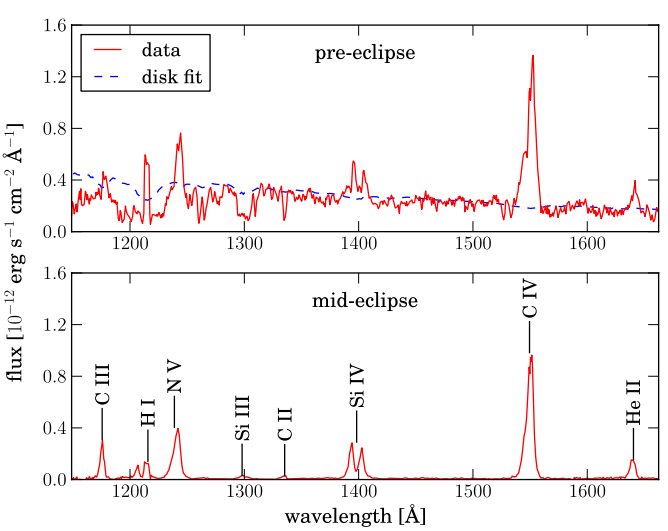
\includegraphics[width=1.0\textwidth]{figures/02-outflows/rwtri_noe.png}
\caption
[UV spectrum of RW Tri in and out of eclipse.]
{
{\sl Credit: Noebauer et al. 2010}.
UV spectrum of RW Tri in and out of eclipse, showing strong lines in 
\civfull\ and \la, among others.
} 
\label{fig:NL_spec}
\end{figure}


The UV spectra of NLs also show strong emission lines, and at 
low to intermediate inclinations dramatic blue-shifted absorption lines
can be seen in some objects. The emission line equivalent widths
in both the optical and the UV show clear correlations with 
inclination \citep{hessman1984,echevarria1988,noebauer}. 
This can be seen clearly in figure~\ref{fig:NL_spec}, and is connected to
the correlation between line strength and absolute magnitude found by \cite{patterson1984};
that is, the decrease in equivalent width at low inclination is caused by an {\em increase}
in continuum flux. This is discussed further in chapters 4 and 6, but also has 
relevance to AGN and quasar unification schemes mentioned later in this introduction.
The optical and UV spectra of NL CVs are discussed further
in the context of winds in chapter 2.

\subsection{Low Mass X-ray Binaries}

Low-mass X-ray binaries (LMXBs) 
are similar to CVs in structure (see figure~\ref{fig:cv_and_xrb}), 
but the compact object
is either a neutron star (NS) or black hole (BH). The accretion disc 
emits in the soft X-ray regime, and an additional hard X-ray power law is also 
seen in the spectrum. This hard component is normally attributed
to Compton up-scattering of seed disc photons by some kind of `corona'
of hot electrons close to the BH \citep[e.g.][]{white1988,mitsuda1989,uttley2014}.
Although I do not study LMXBs directly in this thesis, it is instructive
to briefly discuss of their observational appearance as it is relevant to the links
between accretion and outflow. The discovery that XRBs and CVs follow similar 
tracks on a hardness-intensity diagram \citep{kordingDNjet2008}
is particularly interesting in this regard, especially since \cite{ponti2012}
showed that broad Fe absorption lines are only seen in the soft-state 
high-inclination systems (see section~\ref{sec:xrb_winds}). 
This implies that equatorial outflows are intrinsic to 
the accretion process. Although the driving mechanism
is probably different to CVs \citep[e.g.][]{diaztrigo2015}, 
the similarity in general structure to models for CVs and quasars is striking.


% \begin{figure}
% \centering
% 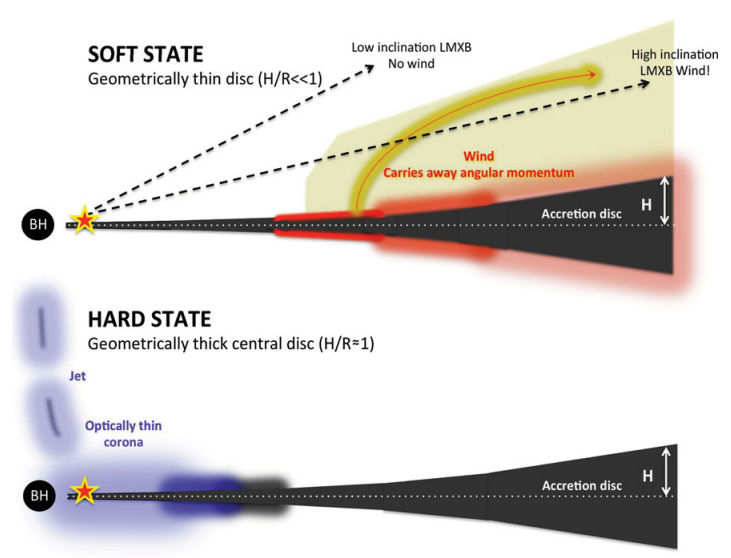
\includegraphics[width=0.7\textwidth]{figures/01-intro/ponti_wind_cartoon.png}
% \caption
% [Hardness intensity diagram for a WD, NS and BH system]
% {
% {\sl Credit: Ponti et al. 2012}
% Hardness intensity diagram for a WD, NS and BH system
% } 
% \label{fig:ponti_cartoon}
% \end{figure}


\section{Quasars and Active Galactic Nuclei}

Spectra of AGN have now been studied for over 100 years, and we have known 
that they exhibit strong, broad emission lines since the first spectrum was taken by
\cite{fath1909}. However, it wasn't until the work of \cite{seyfert1943} that the systematic 
classification of AGN really began, leading to the phrase `Seyfert galaxy'.
This label was applied to galaxies possessing a bright nucleus, spectroscopically
characterised by a blue continuum and a series of strong emission lines.
The first real physical insight into the extraordinary nature of AGN
was provided by \cite{woltjer1959}, who noted that 
(i) the nuclei must have sizes $<100$~pc,
based on the fact that they were unresolved, and (ii) the mass of the nucleus
must be very high, based on virial estimates. 
While both of these observations were based on simple arguments, the fact that these
ultra-luminous celestial objects are both {\em compact} and {\em supermassive}
is perhaps the defining insight into the nature of AGN.

Although the study of AGN was established in the optical waveband, 
radio astronomy also significantly furthered our understanding of AGN
in the mid-20th century. A number of surveys, such as the Cambridge \citep{edge1959}, 
Parkes \citep{ekers1969} and Ohio \citep{ehman1970} surveys discovered a great many 
bright radio point sources distributed isotropically across the sky.
These sources eventually became known as `quasi-stellar radio sources',
or {\em quasars}, and were soon found to be coincident with bright optical
sources or `quasi-stellar objects' (QSOs) at high 
redshifts \citep{schmidt1963,schmidt1965a,schmidt1965b}.
Nowadays, the term quasar normally has very little to do with 
radio emission and is often used interchangeably with QSO. 
Indeed, throughout this thesis I shall refer to a quasar as simply a bright, 
massive AGN; one with sufficiently high luminosity that it dominates the emission 
from its host galaxy.

One of the main classification schemes for AGN is a spectroscopic one, based on 
whether an object possesses broad emission lines in its spectrum, 
such as \civ\, broad \hb\ and
\la, in addition to the narrow lines that are always present. 
If these broad lines are seen, then the AGN is classed as type I;
if not, it is classed as type II (figure~\ref{fig:agn_templates}).
These designations were originally applied to Seyfert galaxies \citep{seyfert1943}, 
but can also be used to classify the more luminous quasar class, despite the apparent
difficulty in finding the expected number of type II sources \citep{zakamska2003}. 
This classification scheme is complicated somewhat by the existence of two
unusual types of AGN: narrow line Seyfert Is (NLSIs), which
may be explained by super-Eddington accretion \citep{done2015} 
or perhaps simply an orientation effect \citep{baldi2016},
and so-called `true type II' AGN, in which the broad line region is absent 
\citep{tran2001,shi2010} rather than obscured (see next section).
Despite this muddying of the waters, what was originally a 
clear dichotomy in spectral type provided a 
profound motivation for attempting to {\em unify} AGN via geometric arguments.


% \subsection{AGN Taxonomy}
% \label{sec:agn_taxonomy}

% In addition to Seyfert galaxies and quasars, there are a number of 
% different classes of AGN. These are broadly characterised by their spectra in the 
% optical, UV and X-ray as well as their radio behaviour. It is worth noting
% that these are observational classifications; that is, even after a century
% of study, the {\em physical} origins of the diverse behaviour of AGN
% are still an active area of research.

\begin{figure}
\centering
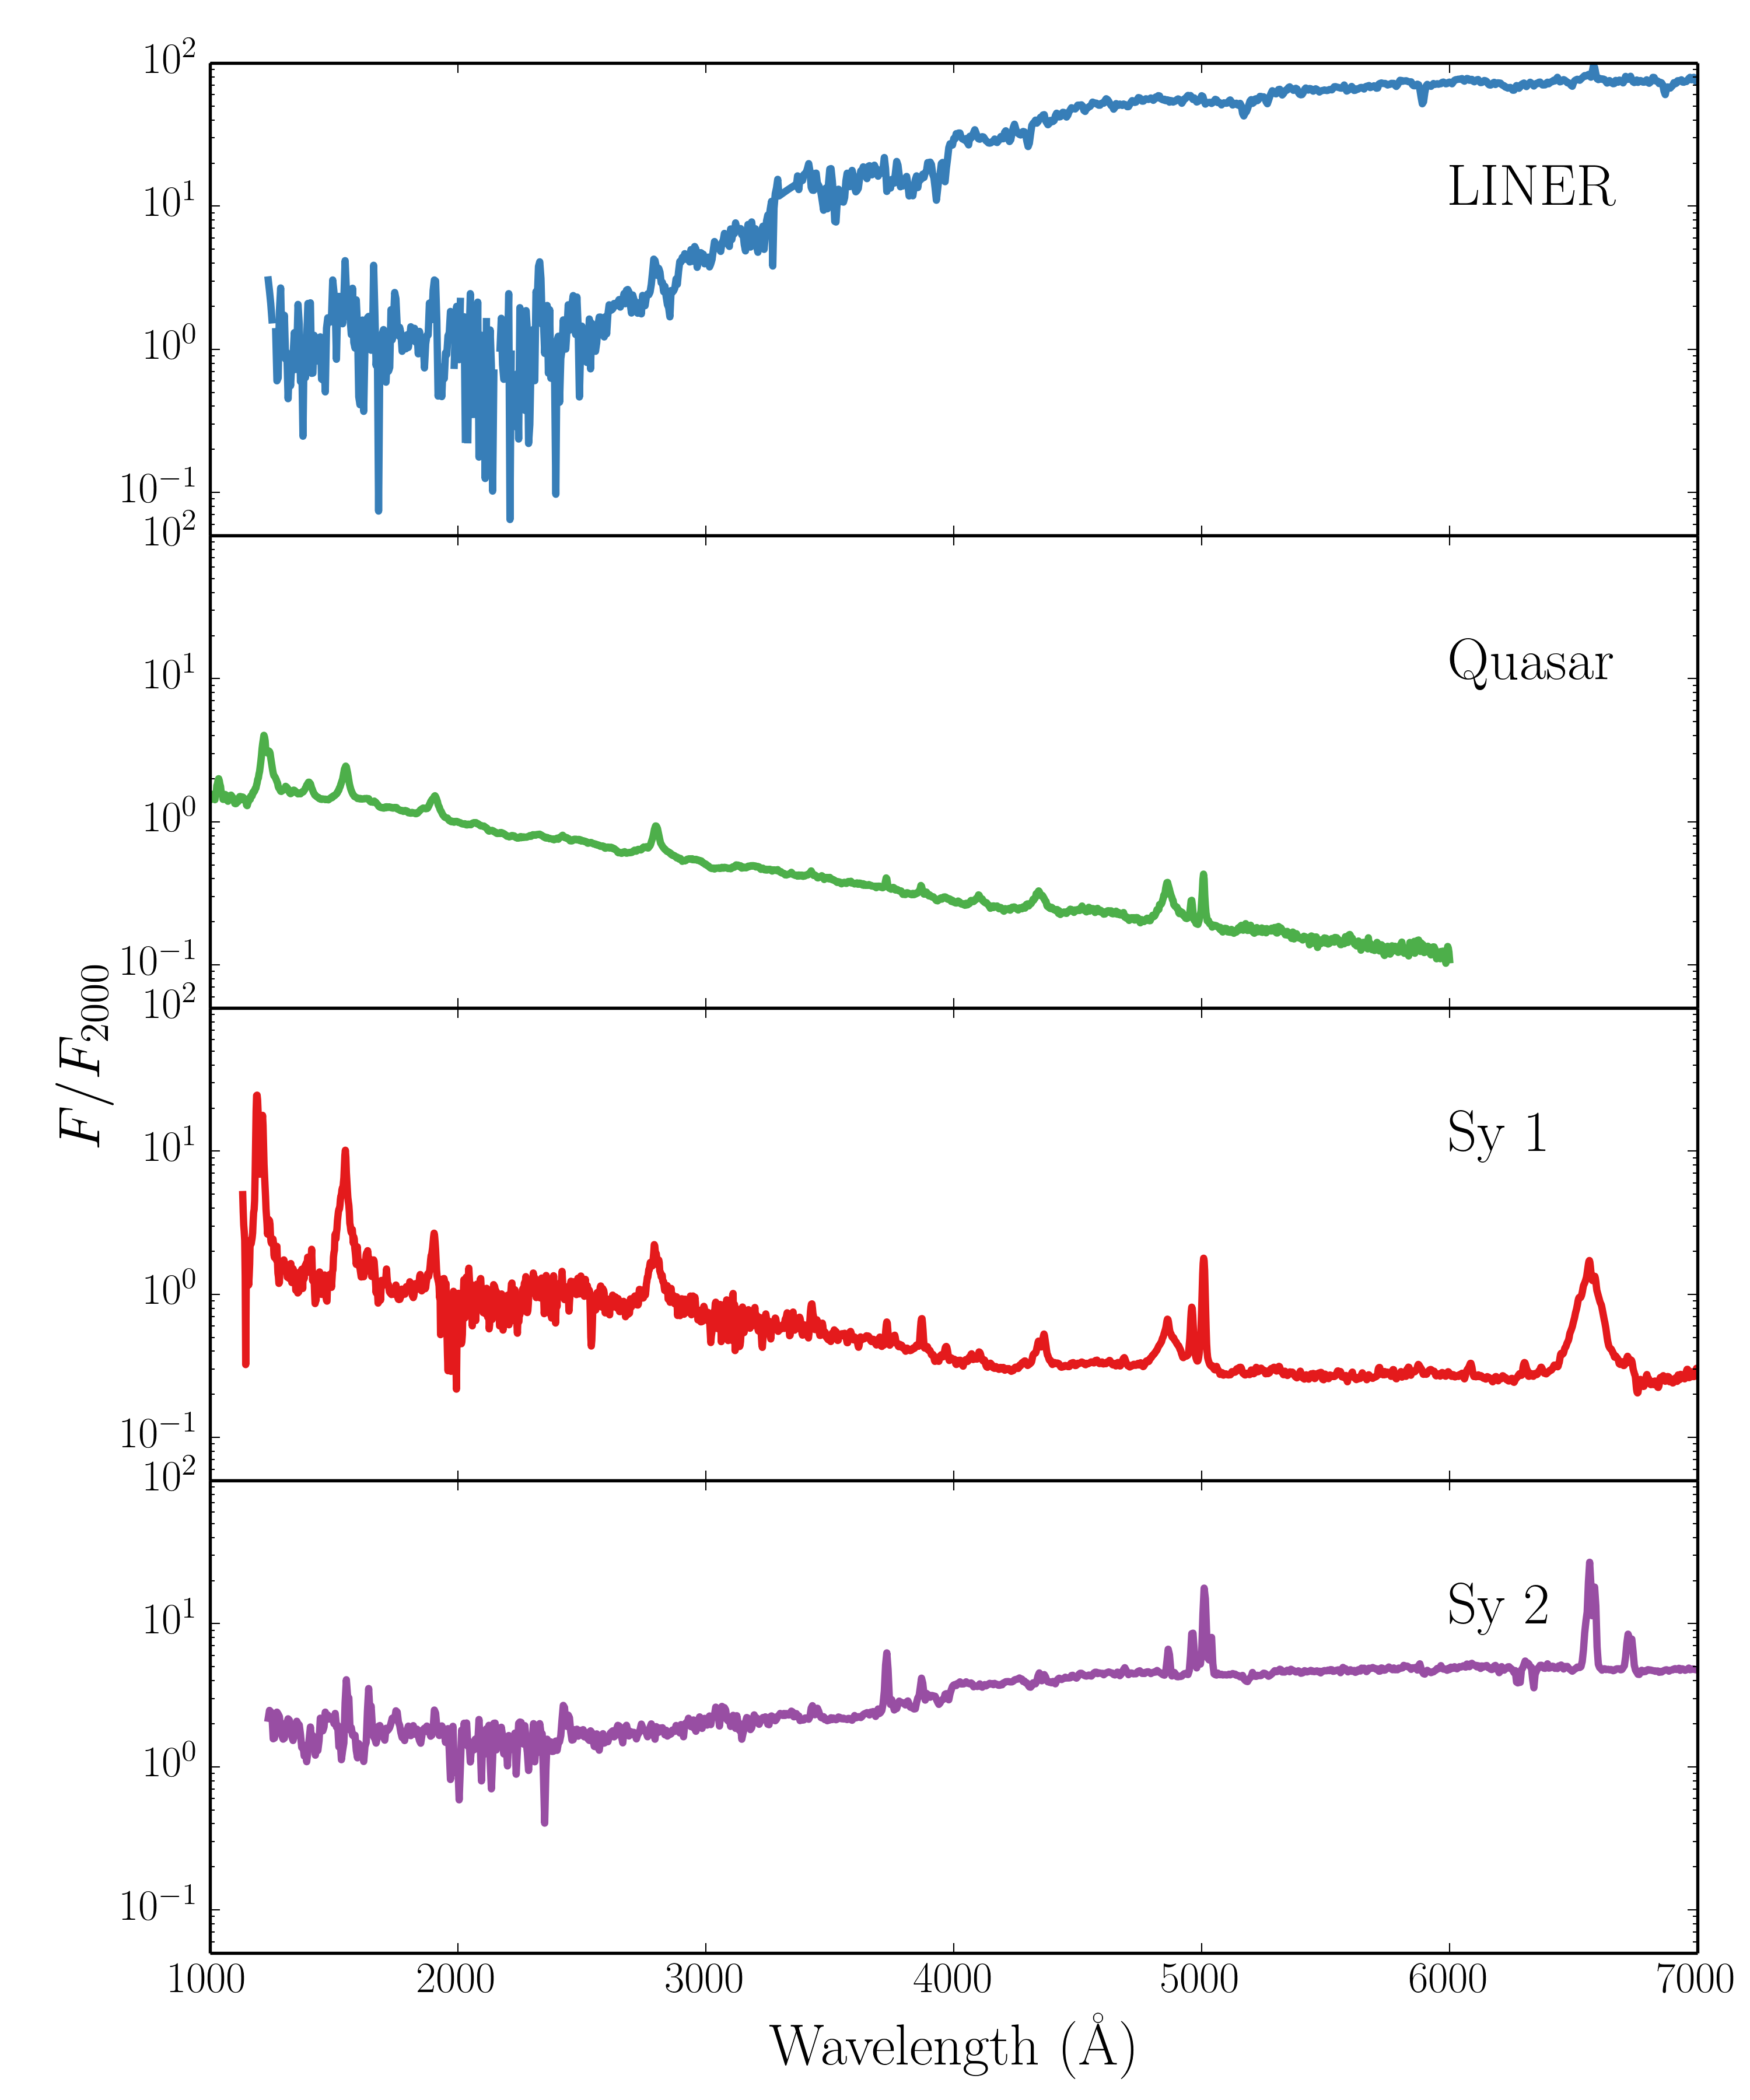
\includegraphics[width=1.0\textwidth]{figures/01-intro/agn_templates.png}
\caption
[Template spectra, from the AGN atlas, for four common types of AGN.]
{
Template spectra, from the AGN atlas, for four common types of AGN.
Obtained from \url{http://www.stsci.edu/hst/observatory/crds/cdbs_agn.html}.
} 
\label{fig:agn_templates}
\end{figure} 

% \subsubsection{Radio Galaxies}

% Radio galaxies are a broad class of AGN, of which radio-loud quasars and blazars are
% technically members, which show strong emission in the radio band. 
% The main classification scheme was proposed by \cite{FR1974}, who split
% sources according to the luminosity. FR I sources are lower in radio luminosity with a steadily decreasing surface brightness towards the edge of the radio lobes.
% FR II sources are more luminous and exhibit bright structures at the edge of their 
% radio maps. Radio galaxies are not particularly relevant here, but it is worth 
% noting that `Radio core dominance', $\log R$, is often used as an orientation indicator 
% \citep{orr1982,wills1995}. This is because more pole-on sources should, in theory, 
% be more dominated by their
% cores whereas edge-on sources should be more dominated by extended radio
% lobes. I discuss the use of orientation indicators further in chapter 6.

% \subsubsection{BL Lacs and Blazars}

% BL Lac objects -- named for the first object of the class, BL Lacertae --
% are AGN with featureless non-thermal continua 
% \citep[see figure~\ref{fig:agn_templates}, and][for a review]{falomo2014},
% in contrast to Seyfert galaxies. 
% Their optical flux is highly polarised \citep{angelstockman1980}
% and they tend to exhibit large-scale optical variability, 
% to the extent that they were originally classified as irregularly variable
% stars \citep{hoff1929}. BL Lacs are a subset of 
% a larger AGN class known as Blazars, the most luminous of which
% are known as optically violent variable (OVV) quasars \citep{wright1998}. 
% Blazars require relativistic beaming in order to explain their high 
% radio luminosities \citep{ghis1985,ghis1993}, 
% implying that the jet is orientated towards
% the observer. These objects thus have an important place in unification
% schemes (see section~\ref{agn_unification}), and
% allow us to measure bulk Lorentz factors in radio jets, which
% can be as high as $\sim50$ \citep{begelman2008}.

% \subsubsection{Obscured and Compton-thick AGN}

% \subsubsection{Low-luminosity AGN}


\subsection{AGN Unification and the dusty Torus}
\label{agn_unification}

Although Seyfert had identified type 1 and 2 AGN, a physical explanation
for this dichotomy was not forthcoming until a study by \cite[][AM85]{antonucci1985}.
They showed unambiguously that the nearby Seyfert 2 NGC~1068 is simply an obscured
type 1 AGN, by finding that broad emission lines appeared in the spectrum of
{\em polarised} flux. This provided the basis for the first successful attempt
to unify AGN behaviour, as it elegantly 
explained the apparent disconnect between the two types of 
AGN as simply a viewing angle effect; at one angle, an observer could look directly
into the broad line region (BLR) near the nucleus, but at Type 2 angles
this region was hidden from view.
The obscuring structure became known as the `torus' \citep{krolik1986}, 
due to its proposed geometry, and it was soon realised that this structure
may be made of dust, in which case it could also be responsible for the infra-red (IR)
bump in AGN \citep{neugebauer1979}.

\cite[][UP95]{UP95} went further than the original unification model
proposed by AM85, as they also tried to account for the dichotomy in 
AGN radio properties (radio-loud/radio-quiet).
The picture they proposed is shown in figure~\ref{fig:unification}.
This model attempts to explain all of the types of AGN 
% described in section~\ref{sec:agn_taxonomy} 
merely as a function of viewing angle
and presence, or absence, of a radio jet. Models such as this also 
describe the series of `bumps' observed in AGN -- the portions
of the spectrum that dominate the luminosity, shown in figure~\ref{fig:quasar_sed}. 
In most models, the `Big Blue Bump (BBB)' is ascribed to thermal 
emission from an accretion disc, and the `Small Blue Bump' to optically 
thin Balmer continuum and Fe~\textsc{ii} emission from the BLR.
The latter can just be seen between $\sim2000$\AA\ and 
$\sim4000$\AA\ in the Seyfert 1 and 
quasar templates in figure~\ref{fig:agn_templates}.
Our understanding of the BBB is still unsatisfactory 
(see section~\ref{sec:disc_continuum}).

\begin{figure}
\centering
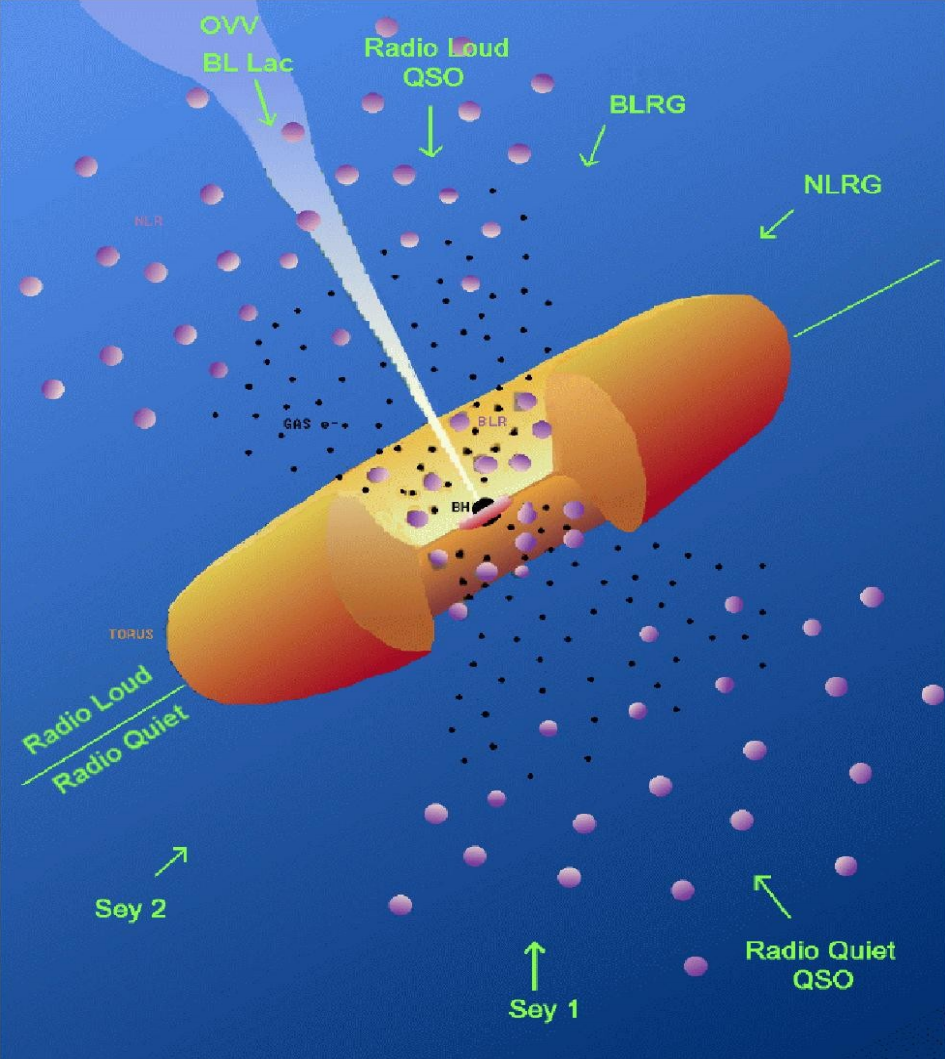
\includegraphics[width=1.0\textwidth]{figures/01-intro/up95.png}
\caption
[A unified scheme for AGN.]
{
A unified scheme for AGN.
} 
\label{fig:unification}
\end{figure} 

\nocite{elvis1994}
\begin{figure}
\centering
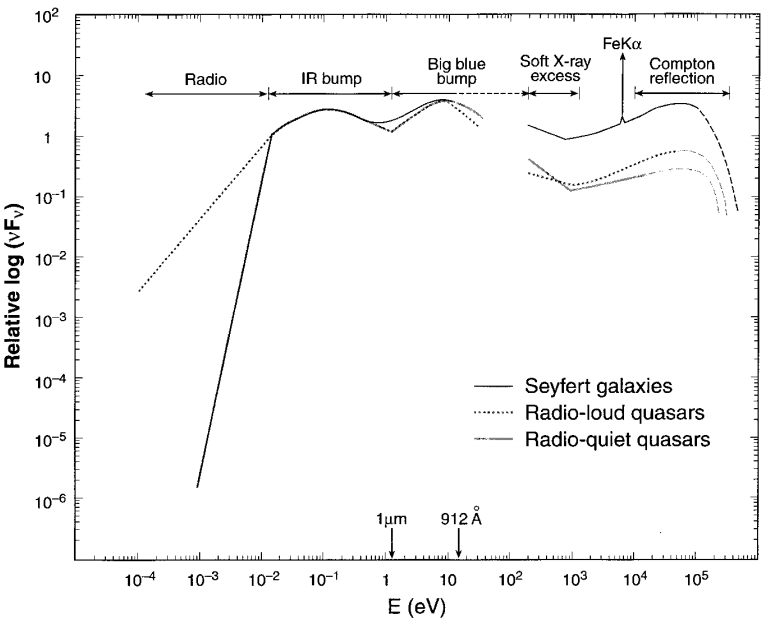
\includegraphics[width=1.0\textwidth]{figures/01-intro/agn_sed.png}
\caption
[Broadband SEDs for different AGN SEDs]
{
{\sl Credit: Koratkar \& Blaes 1999}
Approximate average broadband SEDs for a few types of AGN. The series of 
characteristic bumps can be clearly seen. 
The Soft-X-ray excess is also visible
(see section~\ref{sec:sxxs}).
} 
\label{fig:quasar_sed}
\end{figure}

Since the seminal works by AM85 and UP95, 
the picture has become somewhat more complicated. 
Variable X-ray absorption has been detected in so-called `changing look'
AGN \citep{matt2003,puccetti2007}, including even NGC 1068 itself \citep{marinucci2016}.
Changes in type have also been seen in the optical lines; 
the broad H$\beta$ component in some AGN can dramatically disappear or reappear
\citep[e.g.][]{tohline1976,cohen1986,denney2014}. 
The explanation for this could be variable absorption \citep{elitzur2012}
or a change in the accretion state of the disc. In the latter case,
it has even been suggested that a disc wind could be directly responsible
for this switch \citep{elitzur2014}.
Furthermore, dusty {\em polar} outflows
have been found to be important IR emitters \citep{hoenig2013}, implying
that, even when it comes to dust, the torus is not the whole picture.
Despite these complications, the AGN torus unification picture still
explains a lot of AGN phenomenology, and represents a useful framework 
that can be tested with observations. 


\subsection{X-ray Properties of AGN}

Approximately $10\%$ of the bolometric luminosity of AGN
comes out in the X-ray band, between $\sim0.1$ and $\sim100$~keV.
Thus, AGN dominate the cosmic X-ray background \citep{madau1994}.
The hard X-ray emission typically follows a power law shape with spectral
index -0.9 \citep[e.g.][]{koratkar1999}, 
widely considered, as in LMXBs, to come from a hot `corona' of 
electrons close to the BH that upscatters disc seed photons
\citep[e.g.][]{haardt1991}. The compactness of this X-ray corona
has been confirmed by microlensing \citep{chartas2009, dai2010} 
and variability studies \citep{green1993,crenshaw1996,risaliti2007}. 
Indeed, X-rays in AGN can be highly variable, both in terms of their intrinsic 
X-ray emission, but also due to changes in the absorption characteristics 
\citep{risaliti2002,miller2008,connolly2014}.
I discuss X-ray absorption in more detail, particularly with respect to disc winds, 
in chapter 2.

The hard X-ray spectra AGN also tend to exhibit a number of reflection features. 
Typically, these consist of a strong Fe K$\alpha$ emission line and a `Compton hump'
at high energies. The latter is produced by Compton down-scattering 
of high energy photons \citep{pounds1989,nandra1994}.
It is still unclear exactly where these features originate, 
but a common interpretation is that they are caused by 
reflection off the inner parts of the accretion disc 
\citep{fabian1995,iwasawa1996b,reynolds1999}.
If this is the case, and the broadening of the iron line is relativistic,
this would allow for measurements of the BH spin 
\citep{laor1991,iwasawa1996a,dabrowski1997}.
This hypothesis is somewhat controversial. Multiple authors have found that 
many of the relativistic features supposedly imprinted by BH spin can in fact be explained
by Comptonisation or absorption \citep[e.g.][]{misra1998,miller2013}, 
and radiative transfer modelling has shown that
an outflow can naturally produce the characteristic broad red Fe K$\alpha$ wing \citep{sim2010}.

In Compton-thick AGN, the intrinsic continuum is heavily absorbed with columns of
$N_H\sim10^{24}$~cm$^{-2}$ -- this absorption is normally attributed to the dusty torus, 
but disc winds could also contribute. Compton-thick AGN are required 
in large numbers in order to explain the cosmic X-ray background \citep{setti1989}.
In these sources, reflection features can actually dominate the X-ray spectrum 
\citep{alexander2011,gandhi2013}, but the Fe line is formed from low ionization
stages of Fe on $\sim0.1$~pc scales \citep{gandhi2015}.


\subsubsection{The Soft X-ray Excess}
\label{sec:sxxs}

If one interpolates between the $\nu^{1/3}$ law from the BBB in the UV, and the power law
in the hard X-rays, a curious excess of flux is often found
in type 1 AGN \citep[see figure~\ref{fig:quasar_sed}, and][]{koratkar1999}. 
This is known as the soft X-ray excess (SXXS), which is too 
hot to be explained by thermal disc emission, as a thin disc around an AGN should
never approach the temperatures required. Many models have been proposed to
explain this excess, including relativistically smeared 
photoabsorption \citep{gierlinskidone2004b,gierlinskidone2006}, 
relativistically smeared line and free-free emission \citep{rossfabian2005} 
and a variety of cool Comptonised component geometries such as an 
inner accretion flow \citep{magdiarz1998,done2012} 
and thin layer on top of the disc \citep{januik2001}. 
While the SXXS poses a challenge to
the simplest pictures of AGN, it may also solve some of the issues, as
some of the geometries proposed may help to explain the 
accretion disc size problem discussed in 
section~\ref{sec:disc_continuum} \citep{gardnerdone2016}.

\subsection{The Broad Line Region: Connection to winds and unification}

In the UP95 unification model, the broad emission lines
come from a series of virialised clouds close to the disc plane.
As noted by \cite[][hereafter MCGV95]{MCGV95}, there are a number of problems with
the BLR `cloud' model, perhaps most notably that there is no obvious 
physical origin for such virialised clouds. 
Testing alternative models for the BLR is therefore important.
Indeed, MCGV95 proposed a disc wind model in order to explain both BALs and BELs
in quasars. A disc wind model was also  discussed by \cite{elvis2000}, 
who proposed a structure for quasars that attempted to explain much 
of the behaviour of luminous AGN
merely as a function of viewing angle. Outflow models are discussed further in section~2.
The philosophy of these models is that, before invoking additional
degrees of freedom in a model, we should first test if known quasar phenomenology 
(disc winds) can explain other aspects of their observational appearance.
I have illustrated this general principle with the `Occam's quasar' 
cartoon shown in figure~\ref{fig:occam}. This is the picture that I will
quantitatively test in the latter, quasar-focused sections of this thesis.
The same general principle can also be applied to cataclysmic variables 
and other accreting objects.


\begin{figure}
\centering
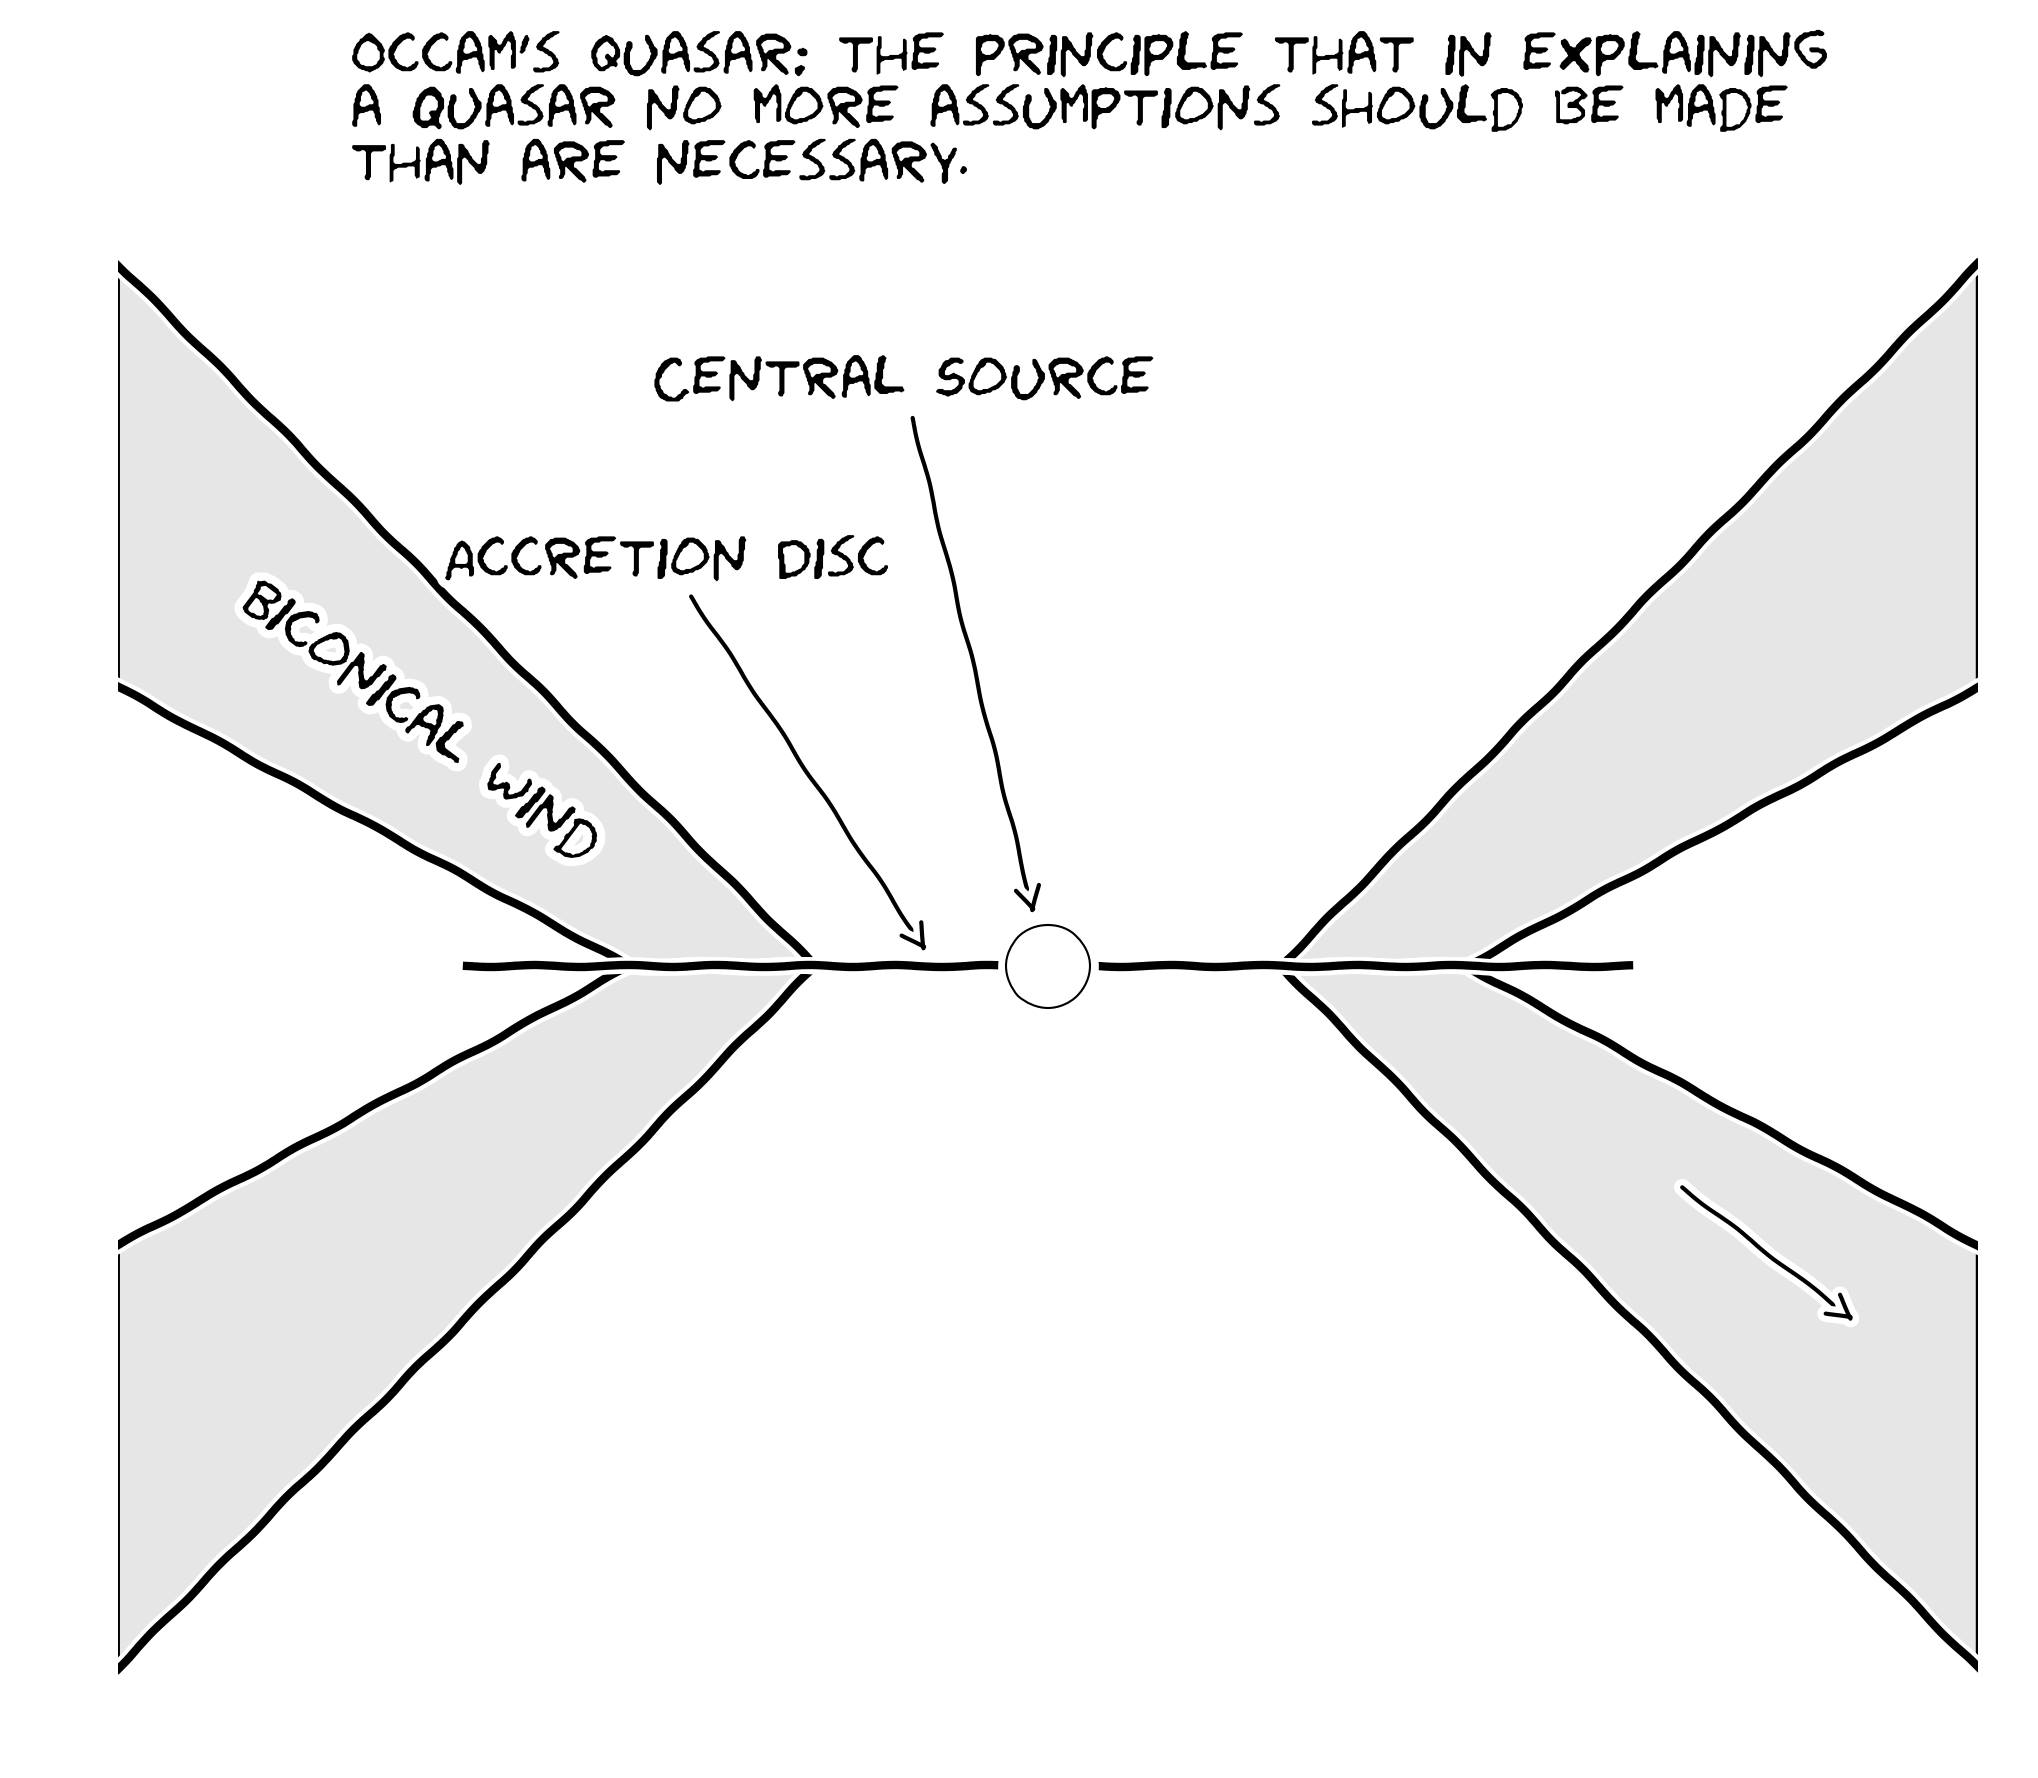
\includegraphics[width=1.0\textwidth]{figures/01-intro/occam.jpg}
\caption
[Occam's quasar]
{
Occam's quasar. How far can this general picture take us when trying to explain
the behaviour of quasars and other accreting compact objects?
} 
\label{fig:occam}
\end{figure}


\section{The Current Understanding of the Disc Continuum}

\label{sec:disc_continuum}

The SS73 model is still the most common way to fit accretion disc spectra and infer
information about the underlying physics. However, 
a number of issues have been raised with the thin-disc model and
its applicability to accreting systems. 

\subsection{The Spectral shape of CV discs}

Attempts to fit the observed SEDs of high-state CVs with simple disc models 
have met with mixed success. In
particular, the SEDs predicted by most stellar/disc atmosphere models 
are too blue in the UV \citep{wade1988,long1991,long1994,knigge1998} and exhibit
stronger-than-observed Balmer jumps in absorption 
\citep{wade1984,haug1987,ladous1989b,knigge1998}. One possible
explanation for these problems is that these models fail to capture
all of the relevant physics. Indeed, it has been argued that a
self-consistent treatment can produce better agreement with 
observational data (e.g. Shaviv et al. 1991;  but see also Idan et al. 2010).
\nocite{idanshaviv2010} \nocite{shaviv1991}
However, an alternative explanation, suggested by Knigge et al.
(1998b; see also Hassall et al. 1985)\nocite{KLWB98,hassall}, 
is that recombination continuum emission from the base of the 
disc wind might fill in the disc's Balmer absorption edge and flatten 
the UV spectrum.

Alternatively, it may just be that CV disks are never really in
a steady state, and so we should only expect the $R^{-3/4}$
temperature profile to hold in a limited portion of the disc.
From eclipse mapping, it has been shown that the inferred accretion
rate increases with radius in NLs \citep{rutten1992, horne1993}.
These results suggest that a non-radiative form of energy loss
is present in the inner regions of the disc, of which potential forms
would be advection or mass loss. This is yet another piece of evidence
that the understanding of accretion and outflow 
are intertwined, although hopefully not inextricably.

\subsection{The Big Blue Bump in AGN}

Does the SS73 model apply well to AGN spectra? There are constrasting views on the matter.
On the one hand, \cite{antonucci2013} claims that ``most of the AGN community is mesmerized by unphysical models that have no predictive power''. 
Yet a recent spectral fitting study by \cite{capellupo2015} concludes that 
``altogether, these results indicate that thin ADs are indeed the 
main power houses of AGN''. So, what are the current problems when 
confronting thin disc models with observation? 

\subsubsection{The Accretion Disc Size Problem}

One of the most interesting results of recent years relating to AGN and accretion discs is
the discovery that the continuum emission region size appears to be
a factor $\sim3$ larger than predicted by standard thin disc theory. This result
has been found independently in both microlensing \citep{morgan2010,dai2010} 
and reverberation \citep{edelson2015} studies, and poses a challenge to the 
current best-bet model for the big blue bump in AGN. 
One proposed solution is that the discs in AGN are inhomogenous,
consisting of individual clumps with independently
varying temperatures \citep{dexteragol2011}, but this is very much
still an active area of research. It is worth noting that the impact
of winds on these results has not yet been properly quantified, something
our team is currently trying to address \citep{mangham}.

\subsubsection{Fitting AGN Spectra and the 1000\AA\ Break}

One of the {\em successes} of the thin disc model, when applied to AGN,
is that we do observe a slope in the UV of $\alpha_{UV} = 0.32$, confirming
the theoretical prediction of $\nu^{1/3}$. 
However, AGN spectra do not exhibit the {\em overall} spectral shape 
\citep[e.g.][]{davis2007,shankar2016} or colour-mass scalings \citep{bonning2007} 
expected from theoretical predictions. 
This can be seen clearly in figure~\ref{fig:agn_templates},
where both the quasar and Seyfert spectra tend to peak in the UV, rather than
the EUV. Furthermore, there is a characteristic break in AGN spectra at
around $1000$~\AA\ \citep{lusso2015}, which does not scale with BH mass or luminosity,
as one might expect for a break associated with an accretion disc. 
There is also no evidence in AGN of the expected polarisation signatures from an 
optically thick disc atmosphere \citep{stockman1979,antonucci1988,antonucci1996}. 

Despite these problems, recent work suggests that the thin disc model 
still has some potential. \cite{capellupo2015} were able to fit a number of
AGN spectra in the UV and optical with thin disc models, although successful fits
were only found once they included effects such as Comptonisation and mass-loss,
as well as correcting for extinction. BH spin also had a reasonable effect on the 
spectral fits, although it is somewhat difficult to constrain from spectral fitting alone.
The $1000$~\AA\ break has also been explained with a mass-losing disc \citep{laordavis2014},
and \cite{lusso2015} suggested that incorrect IGM corrections 
may be exacerbating the effect.
So, while many problems exist, it may not quite be time to 
abandon the Shakura-Sunyaev ship just yet.

\section{The Universality of Accretion}

Accretion appears to be an important physical processes across $\sim10$ orders
of magnitude in mass. But is this process the same on all scales? Does any 
behaviour manifest in all accreting systems? 

\subsection{The RMS-flux relation}

Broad-band variability is common in all types of accretion disc. It has been
known for some time that there exists a linear relationship
between the flux and absolute root-mean-square (rms) amplitude
of this variability. This was discovered first in XRBs and AGN 
\citep{uttley2001, uttley2005, heil2012}, but it has been shown
more recently that the relationship extends to CVs and even YSOs 
\citep{scaringi2012,scaringi2015a}. The relationship is also not limited
to just one type of CV but is present in both NLs and DNe \citep{vandesande2015}.
 
The model that best reproduces this behaviour is the so-called
`fluctuating accretion disc' model \citep{lyubarskii1997,kotov2001,
arevalo2006,hogg2015}. More generally,
additive processes cannot reproduce this behaviour, and a multiplicative
mechanism is required \citep{uttley2005}. 
Regardless of the mechanism, the rms-flux relation is one of the most
clear-cut examples of a universal accretion phenomenon. 
It tells us that at least some of the behaviour in CV discs
is also present in AGN and XRBs, strengthening the argument that CVs
can be used as `accretion laboratories'. 


\subsection{Accretion states and disc-jet coupling}
\label{sec:disc-jet}

Variable and transient sources are common in astrophysics, particularly
when the sources are accreting. I have already mentioned the DIM an
and its applicability to LMXBs and CVs; it turns out that when one plots
the colour and luminosity evolution over the course of an ourburst cycle 
then they follow very similar tracks \
citep[see figure~\ref{fig:kording_hid}, ][]{kordingDNjet2008}.
The detection of radio jets is also intrinsically linked to the accretion state
of the system (disc-jet coupling), as jets only appear in the `hard' accretion 
state, to the right of the so-called `jet line' \citep{fender2001,fender2004}.
\cite{kordingDNjet2008} showed that this behaviour also occurs in CVs, 
as radio emission in the DN SS Cyg is also detected in the same region 
of colour-luminosity space. There is also a well-known correlation between 
radio and X-ray luminosities in low-hard states \citep{gallo2003}.

This clear correlation with accretion state on HIDs has natural parallels 
with AGN. 


The jet production mechanism in BHs in general is not well known. 
Theoretical work suggests that radio jets should be correlated with BH spin 
\citep{penrose1971,blandford1977}, 
but whether such a correlation exists in LMXBs is 
controversial \citep{fender2010,narayan2012}.
This has significant implications for AGN; if powerful radio jets are 
associated exclusively with rotating BHs then the number of radio-loud AGN
would imply a large fraction of them must be rapidly spinning, with
high radiative efficiencies. 
Further evidence that radio jets are not simply produced by RIAFs onto spinning
BHs is found when one considers that NLs show evidence of synchrotron
radio emission \citep{coppejans2015}. This important result suggests that our understanding
of jets is incomplete, and that the links between accretion state and 
jet production are fundamental, but unsolved. Disc winds may complicate, or simplify,
matters, depending on one's outlook (see chapter 2).

\begin{figure}
\centering
\includegraphics[width=1.0\textwidth]{figures/01-intro/kording_hid.png}
\caption
[Hardness-intensity diagrams for three types of accreting objects.]
{
{\sl Credit: Kording et al. 2008.} 
Caption.
} 
\label{fig:kording_hid}
\end{figure}

\subsection{A Global Picture}

Clearly, accretion physics is relevant to a plethora of astrophysical phenomena, 
and at least some of the physics of accretion is applicable to {\em all} 
classes of accreting object. 
It would also appear that the outflowing material observed in accreting systems 
has a profound effect on the accretion process itself, and 
possibly significantly affects the observational 
appearance of disc-accreting systems (c.f. Elvis unification model). 
Hence, in the next chapter, I will review the evidence for
winds and discuss some of the relevant background theory.

 % Introduction


% %\chapter{Accretion}

% \epigraph{``And now, I shall talk about the most efficient process in the universe. No, not bureaucracy..."}
% {--- \textup{Petri Savoleinen}, A talk at the Harvard-Smithsonian CfA}

As described in the Introduction, there are a wide variety of accreting systems
with varying degrees of astrophysical significance. Here I will describe the 
physics of accretion in more detail, before discussing the theoretical and observational 
basis for accretion disc winds. 

\section{The Physics of Accretion}

The basic phenomenon of accretion- matter falling into a gravitational potential well- 
is a ubiquitous one in astrophysics. 


\subsection{Roche Lobe-Overflow}

In binary systems, there are only two ways by which matter can transfer 
from the secondary to the compact object. One is by Roche Lobe-overflow (RLOF),
whereby stellar evolution causes the donor star to fill it's Roche Lobe, the surface
of equipotential around the star. The alternative is that a radiatively driven wind
may expel stellar material from the donor, allowing some of it to flow onto the compact object.
Although stellar wind accretion is common in some classes (REFs), here I will focus on 
RLOF as it is more common in the systems that commonly exhibit high-state accretion discs
and associated outflows.

The Roche potnetial, $\Phi_R$, can be expressed as ?



\subsection{Accretion discs}

The basic phenomenon of accretion- matter falling into a gravitational potential well- 
is a ubiquitous one in astrophysics. The details of how and where the energy is released
and how angular momentum is transported is subject to a number of different 
interpretations, mainly depending on the {\em geometry} of the accretion flow.




The so-called $\alpha$-disc model developed by \cite[][hereafter SS73]{shakurasunyaev1973} is
currently the leading candidate for explaining how energy and angular momentum
is transported an accretion disc. The starting point for this model is the parameterisation
of viscosity using a simple form of
\begin{equation}
\nu = \alpha c_s H.
\end{equation}
Viscous torques then allow the conversion of orbital kinetic energy into heat, which 


By considering the energy released through viscous dissipation 
in the disc it is possible to derive a temperature distribution as a function of 
radius \citep{shakurasunyaev1973, fkrbook}. 

\begin{equation}
T(R) =  
\end{equation}

It is important to recognise that the work of \cite{shakurasunyaev1973} 
{\sl does not specify the nature of the disc SED}. What it does do is 
say where energy is originally released. Typically,
accretion discs are modelled as a series of annuli each emitting 
as blackbodies, but it is possible that a disc atmosphere with frequency-dependent
opacity would create a somewhat different spectrum. It is also possible that {\em neither} of these 
treatments are realistic. We shall therefore devote a little time to discussing
the observational arguments for accretion discs and the current problems 


\section{Observational Appearance}



\subsubsection{Potential Problems with the Thin-disc model}

A number of issues have been raised with the thin-disc model and
its applicability to accreting systems. 

\subsubsection{Quasar emission region sizes from microlensing}

\subsubsection{Quasar emission region sizes from X-ray lags}

\subsubsection{The Spectral shape of CV discs}

Attempts to fit the observed SEDs of high-state CVs with simple disc models have met with mixed success. In
particular, the SEDs predicted by most stellar/disc atmosphere models 
are too blue in the UV \citep{wade1988,long1991,long1994,knigge1998} and exhibit
stronger-than-observed Balmer jumps in absorption 
\citep{wade1984,haug1987,ladous1989b,knigge1998}. One possible
explanation for these problems is that these models fail to capture
all of the relevant physics. Indeed, it has been argued that a
self-consistent treatment can produce better agreement with 
observational data (e.g. Shaviv et al. 1991;  but see also Idan et al. 2010).
\nocite{idanshaviv2010} \nocite{shaviv1991}
However, an alternative explanation, suggested by Knigge et al.
(1998b; see also Hassall et al. 1985)\nocite{KLWB98,hassall}, 
is that recombination continuum emission from the base of the 
disc wind might fill in the disc's Balmer absorption edge and flatten the UV spectrum.

\section{The Universality of Accretion}

Accretion appears to be an important physical processes across $\sim9$ orders
of magnitude in mass. But is this process the same at all scales? Does any 
behaviour manifest in all accretion systems? 

\subsection{The RMS-flux relation}

Broad-band variability is common in all types of accretion disc. It has been
known for sometime that there exists a linear relationship
between the flux and absolute root-mean-square (rms) amplitude
of this variability. This was discovered first in XRBs and AGN 
\citep{uttley2001, uttley2005, heil2012}, but it has been shown
more recently that the relationship extends to AWDs and even YSOs 
\citep{scaringi2012,scaringi2015a}. The relationship is not limited
to one type of AWD, as it is present in both NLs and DNe \citep{vandesande2015}.
 
The model that best reproduces this behaviour is the so-called
`fluctuating accretion disc' model (REFs). It has been shown that 
additive processes cannot reproduce the behaviour, and a multiplicative
mechanism is required (REFs). 
Regardless of the mechanism, the rms-flux relation is one of the most
clear-cut examples of a universal accretion phenomenon. 
It tells us that at least some of the behaviour in AWD discs
is present in AGN and XRB, strengthening the argument that AWDs
should be used as `accretion laboratories'. 


\subsection{Accretion States}


\begin{figure}
\centering
\includegraphics[width=0.7\textwidth]{figures/02-accretion/kording_hid.png}
\caption
{
{\sl Credit: Kording et al. XXXX.} 
Caption.
} 
\label{fig:kording_hid}
\end{figure}



\subsection{Jets and Outflows}


\subsection{A Global Picture}

Clearly, accretion physics is relevant to a plethora of astrophysical phenomena. 
It would also appear that the outflowing material observed in accreting systems 
has a profound effect on the accretion process itself, as well as acting 
as a spectral `filter' -- modifying, and sometimes dominating the observational 
appearance of accretion discs. % Background Theory 
% \newpage
% \lhead{\emph{2. Accretion Disc Winds}}  % Set the left side page header to "Contents"

\chapter{Accretion Disc Winds}
\label{sec:winds}

\epigraph{``A view of space, with an elephant obstructing it"}
{{\sl Mike Vennart, Silent/Transparent}}


%%%%WINDS 
%%% COULD MAKE THIS A NEW CHAPTER
\section{Observational Evidence}

The observational evidence for mass-loaded outflows or winds is 
widespread across the entire astrophysical mass range and most of
the electromagnetic spectrum. Before detailing the more compelling aspects
of this evidence, it is pertinent to briefly discuss the `smoking gun'
used to unambiguously detect winds -- the presence of blue shifted BALs
or `P-Cygni' profiles in an objects spectrum. 

Figure~?? shows how a spherical outflow of significant opacity will 
cause these characteristic line profile shapes to form, as scattering out of the line of sight 
causes a dip in the blue wing of the line, while scattering into the 
line of sight from other portions of the outflow causes an increase in flux
in the red wing of the line. The situation is much more complex in most
astrophysical situations; for example, the geometry is rarely spherically 
symmetric, and the line is rarely a pure scattering case. Indeed, the potential 
for complicated radiative transfer effects and variety in line formation mechanisms
is one of the reasons why 3D Monte Carlo radiative transfer simulations are necessary
to effectively model disc winds (see section 3).

\subsection{Cataclysmic Variables}

It has been known for a long time that winds emanating from the
accretion disc are important in shaping the ultraviolet (UV) spectra
of high-state CVs \citep{heap1978, greensteinoke1982}. The most spectacular evidence for such
outflows are the P-Cygni-like profiles seen in UV resonance lines such as
\civfull\ \citep[][; see figure~\ref{fig:cordova}]{cordova1982}). 
Considerable effort has been spent over the
years on understanding and modelling these UV features 
\citep[e.g.][]{drewverbunt1985,maucheraymond1987,SV93,KWD96,
kd1997,knigge1997,LK02,noebauer,puebla2011}. 
The basic picture emerging from these efforts is
of a slowly accelerating, moderately collimated bipolar
outflow that carries away $\simeq 1\% - 10\%$ of the accreting
material. State-of-the-art simulations of line formation in this type
of disc wind can produce UV line profiles that are remarkably similar
to observations, as shown in figure~\ref{fig:zcam_lk02}.

\begin{figure}
\centering
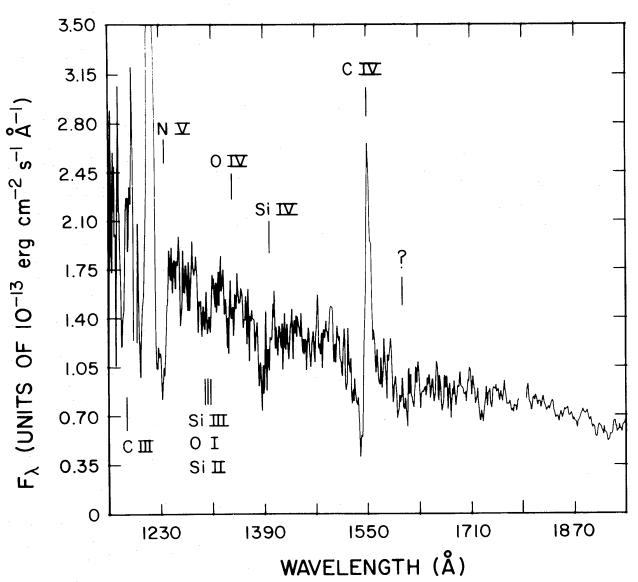
\includegraphics[width=0.8\textwidth]{figures/02-outflows/cordova_mason.png}
\caption
{
{\sl Credit: Cordova \& Mason 1982}. 
UV spectrum of the DN TW Vir during outburst. The P-Cygni profiles
can be seen clearly, demonstrating that a strong, fast outflow is present
in the system. 
} 
\label{fig:cordova}
\end{figure}

\begin{figure}
\centering
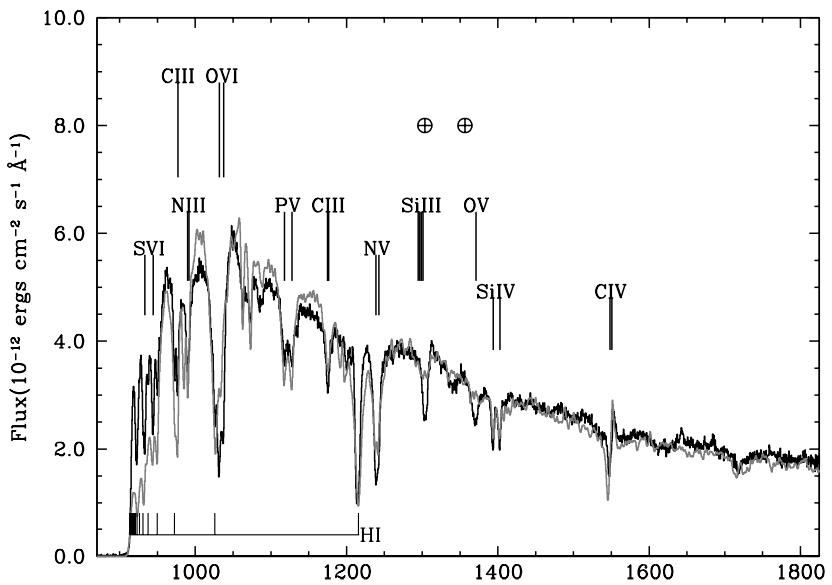
\includegraphics[width=0.8\textwidth]{figures/02-outflows/zcam_lk02.png}
\caption
{
{\sl Credit: Long \& Knigge 2002}. 
UV spectrum of Z Cam, compared to a synthetic spectrum from MCRT simulations.
} 
\label{fig:zcam_lk02}
\end{figure}

Much less is known about the effect of these outflows on the optical
spectra of high-state CVs. Direct evidence of wind-formed lines comes from
isolated observations of P-Cygni-like line profiles in
\ha\ and He \textsc{i} $\lambda5876$, \citep{patterson1996, RN98, kafka2004}. 
However, the effect on
the {\em emission} aspects of the optical spectrum is not well known.
\cite{MC96, MC97} have shown that the presence of disc winds may
offer a natural explanation for the single-peaked optical emission lines in
high-state CVs, since they can strongly affect the radiative transfer
of line photons (see figure~??). Stronger support for a significant wind contribution to the
optical emission lines comes from observations of eclipsing
systems. There, the single-peaked lines are often only weakly
eclipsed, and a significant fraction of the line flux remains visible
even near mid-eclipse \citep[e.g.][]{baptista2000,groot2004}. 
This points to line formation in a spatially
extended region, such as a disc wind (see section~\ref{novalikes}).
It is also possible that a wind may affect the continuum emission of CVs,
as described in section~??. The effect of an accretion disc wind
on the optical line and continuum emission of CVs is addressed directly,
via radiative transfer modelling, in chapter 4.

% These spectra are typically characterized
% by H and He emission lines superposed on a blue continuum. In many
% cases, and particularly in the SW~Sex subclass of NLs
% \citep{HSK86,DR95}, these lines are single-peaked. This is contrary to
% theoretical expectations for lines formed in accretion discs, which
% are predicted to be double-peaked \citep{smak1981, hornemarsh1986}. 
% {\em Low-state} CVs (dwarf novae in quiescence) do, in fact,
% exhibit such double-peaked lines \citep{marshhorne1990}. 

% Could disc winds also have an impact on the UV/optical {\em continuum}
% of high-state CVs? This continuum is usually thought to be dominated
% by the accretion disc and modelled by splitting the disc into
% a set of concentric, optically thick, non-interacting annuli following
% the standard $T_{eff}(R) \propto R^{-3/4}$ radial temperature
% distribution \citep{shakurasunyaev1973}. In such
% models, each annulus is taken to emit either as a blackbody or,
% perhaps more realistically, as a stellar/disc atmosphere model
% \citep{Schwarzenberg-Czerny1977,wade1984,wade1988}.
% In the latter case, the local surface gravity, $\log{g}(R)$, is
% assumed to be set solely by the accreting WD, since self-gravity is
% negligible in CV discs.

\subsection{X-ray Binaries}
\label{sec:xrb_winds}

Like CVs, evidence for fast outflows in LMXBs is not constrained to 
a single waveband. UV absorption in outflows was detected when
\cite{ioannau2003} observed \civfull\ P-Cygni profiles with blueshifts 
of $\sim1500$km~s$^-1$. Shortly after, a series of papers found 
highly ionized Fe absorption with similar blueshifts and FWHM of around 
$1500$km~s$^-1$ (REFs). These absorption features tended to be detected
in high-inclination, `dipping' LMXBs, and this was confirmed in more sources
by \cite{ponti2012}, who proposed an equatorial geometry based on this (see 
figure~??). The same study demonstrated (figure~??) that
the winds only appeared in the soft, 
disc dominated accretion state, on the opposite side of the HID to the
region where jets are common. This exciting result demonstrated how
important winds are to our understanding of accretion, and required that
we expand the discussion of accretion states to include `disc-jet-wind' 
coupling.

\begin{figure}
\centering
\includegraphics[width=1.0\textwidth]{figures/01-intro/ponti_hid.png}
\caption
{
{\sl Credit: Ponti et al. 2012}. 
HID demonstrating that winds appear in the soft states of LMXBs.
} 
\label{fig:ponti_hid}
\end{figure}

\begin{figure}
\centering
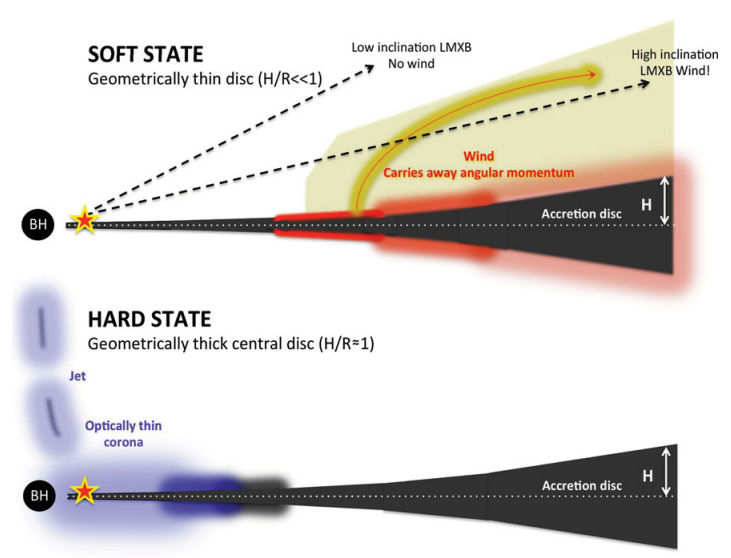
\includegraphics[width=1.0\textwidth]{figures/01-intro/ponti_wind_cartoon.png}
\caption
{
{\sl Credit: Ponti et al. 2012}. 
A cartoon illustrating the expected geometry of soft-state LMXB winds.
} 
\label{fig:ponti_hid}
\end{figure}


\subsection{AGN and Quasars}
\label{sec:agn_winds}

\subsubsection{Broad Absorption Line Quasars}

\subsubsection{Warm Absorbers}

\subsubsection{Ultra-fast Outflows}


\begin{figure}
\centering
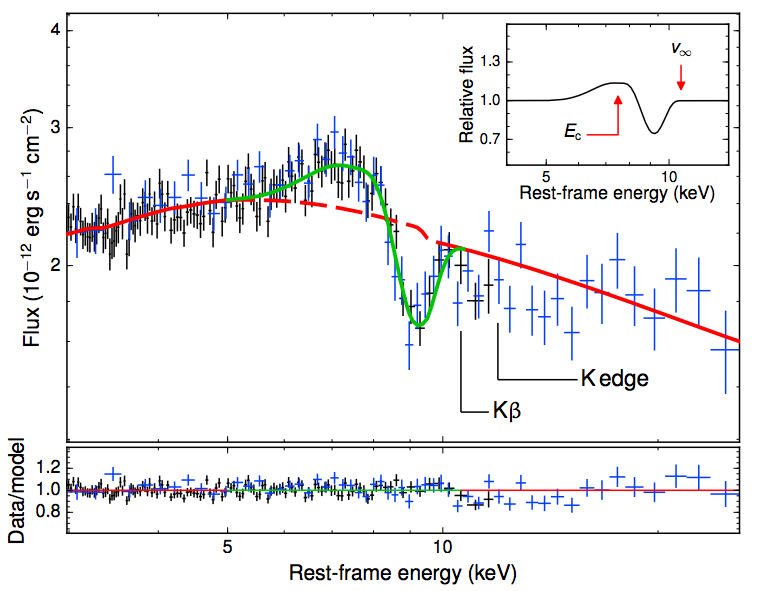
\includegraphics[width=1.0\textwidth]{figures/02-outflows/nardini_pds456.png}
\caption
{
{\sl Credit: Nardini et al. 2015}. 
X-ray spectrum fitted with a P-Cygni profile from a spherical outflow model.
{\sl XMM-Newton} data is shown in black with two combinaed {\sl NuStar}
observations in blue.
} 
\label{fig:nardini}
\end{figure}


\subsection{Stellar Winds}

Although stellar winds are clearly not accretion disc winds,
they provide a useful, and better understood, testing ground for much
of the physics of radiatively-driven outflows.

\subsubsection{Clumping}




\section{Driving Mechanisms}

Let us consider a parcel of ideal gas. By imposing nothing more than
conservation of mass, energy and momentum on that parcel we can write down
three equations of hydrodynamics
\footnote{I stress that these equations are not used in hydrodynamic
simulations in this thesis (see section ?, for example); 
they are discussed here because they provide a natural reference point
for exploring potential driving mechanisms for winds in accreting systems.
}

\begin{equation}
\label{eq:continuity}
\frac{D \rho}{Dt} + \rho \nabla \cdot \vec{v} = 0
\end{equation}

\begin{equation}
\label{eq:motion}
\rho \frac{Dv}{Dt} = -\nabla P + \frac{1}{4 \pi}(\nabla \times \vec{B}) \times \vec{B} + \rho \vec{F}_{rad} + \rho \vec{g}
\end{equation}

\begin{equation}
\label{eq:energy}
\rho \frac{D}{Dt} \left(\frac{e}{\rho}\right) = P \nabla \cdot \vec{v} + \rho \cal{L}
\end{equation}

Here $D$ denotes a derivative within the comoving frame of the gas parcel, $\vec{v}$ is the velocity,
$\rho$ is the gas density, $\vec{B}$ is the local magnetic field, $\vec{F}_{rad}$ is the radiation
force per unit mass and $\vec{g}$ denotes the gravitational acceleration vector.
Equation~\ref{eq:continuity} is the {\em continuity equation} and describes conservation of mass. 
Equation~\ref{eq:motion} is the {\em equation of motion} and describes conservation of momentum.
Equation~\ref{eq:energy} is the {\em equation of energy conservation}. 
We can use equation~\ref{eq:motion} to neatly demonstrate how an outflow can be driven. I have 
deliberately written the equation so that all the force terms lie on the RHS. We can then see that
for an outflow to be driven from an accreting object one simply needs one of the terms on
the RHS to dominate over gravity, $\rho \vec{g}$. These terms thus signify three potential
driving mechanisms.

\begin{itemize}
	\item Magnetic Forces, $\frac{1}{4 \pi}(\nabla \times \vec{B}) \times \vec{B}$.
	\item Radiative Forces, $\rho \vec{F}_{rad}$.
	\item Thermal Pressure, $-\nabla P$.
\end{itemize}

We can now examine under what physical conditions (and in which corresponding astrophysical objects)
we might expect these forces to overcome gravity and cause a parcel of mass to escape to infinity.
In other words: {\em what might drive a wind?}

\subsection{Thermal Winds}

In hydrostatic equilibrium (HSE), thermal pressure balances gravity and no other forces 
are present, meaning that the equation of motion can be written as 
\begin{equation}
\label{eq:hse}
\rho \frac{Dv}{Dt} = -\nabla P +  \rho \vec{g} = 0
\end{equation}
Clearly, if the thermal pressure is then significantly 
increased then this equilibrium condition no longer holds. 
This can occur in accretion discs at temperatures in excess of $\sim10^7$~K --
where other forces are negligible compared to thermal pressure -- 
and where the escape velocities are relatively low (i.e. far out in the disc).
Due to the temperature and gravity scalings, this means
that XRBs are natural candidates for showing evidence of thermally driven
winds. The outer disc can be heated to the Compton temperature by the central X-ray source,
potentially driving relatively high mass-loss rate outflows \citep{begelman1983,woods1996}. 
This driving mechanism has been proposed as a natural explanation
for the ever-present equatorial outflows in soft state XRBs \citep{ponti2012}.
However, they are much less likely candidates in CVs and AGN {\bf Discuss scaling
arguments with equations?}.


\subsection{Radiatively Driven Winds}
\label{sec:rad_winds}

\subsection{Line-driven Winds}

\subsection{Magneto-centrifugal Winds}

\section{Accretion Disc Wind Models}


\section{A Kinematic Prescription}




\section{The really, really big picture: AGN Feedback}

The event horizon of a $10^9~M_\odot$ BH is approximately 
$10^{15}$~cm, a billionth of the size of a typical galactic bulge. This is 
roughly the difference in size between a small coin and the radius of the 
Earth. Despite this vast different in scale, there are multiple
pieces of evidence that the physics on the scale of the gravitational
radius of the BH really does affect the evolution and dynamics of its host galaxy.
I shall briefly discuss the evidence for this statement, and 
assess the potential role of winds together with alternative mechanisms.

\subsection{Observational evidence for feedback}

Perhaps the most famous pieces of evidence for some kind of long-distance 
relationship between a central BH and its host galaxy are the 
$M_{BH}-\sigma_*$ and $M_{BH}-M_{bulge}$ correlations, shown in figures~\ref{fig:msigma}
and \ref{fig:mbulge} respectively.

\nocite{mcconnell2013,gultekin2009}
\begin{figure}
\centering
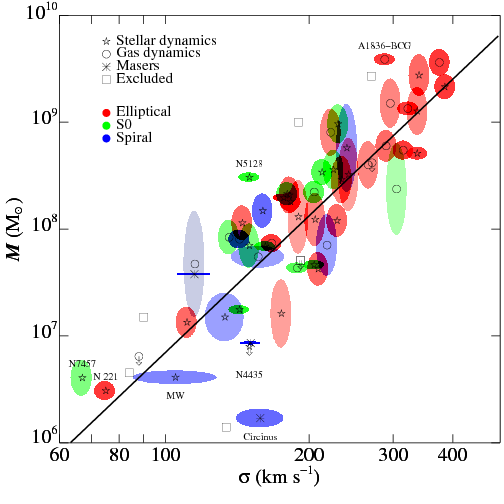
\includegraphics[width=0.7\textwidth]{figures/02-outflows/msigma.png}
\caption
{
{\sl Credit: Gultekin et al. 2009}. 
The $M_{BH}-\sigma_*$ correlation.
} 
\label{fig:mbulge}
\end{figure}

\begin{figure}
\centering
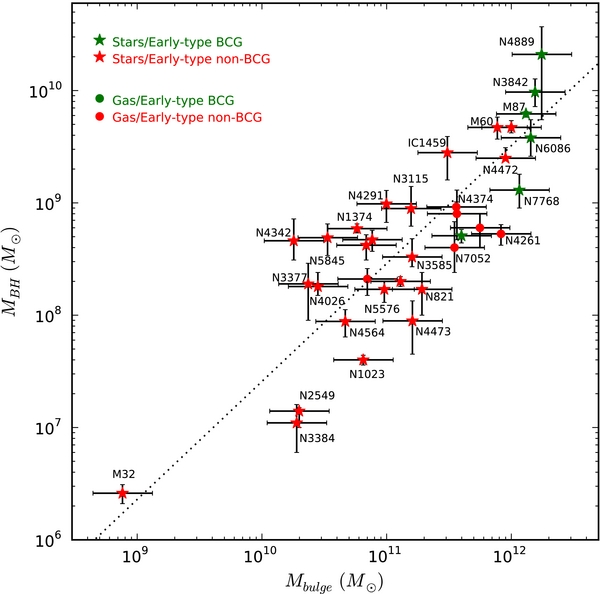
\includegraphics[width=0.7\textwidth]{figures/02-outflows/mbulge.jpg}
\caption
{
{\sl Credit: McConell \& Ma 2013}. 
The $M_{BH}-M_{bulge}$ correlation.
} 
\label{fig:mbulge}
\end{figure}

\subsection{Radiative or quasar mode feedback}

\subsection{Kinetic or radio mode feedback}

\subsection{In-situ Explanations}


 % Experimental Setup


% \newpage
% \lhead{\emph{3. Radiative Transfer and Ionization}}  % Set the left side page header to "Contents"

% \chapter{Radiative Transfer and Ionization}

\epigraph{``I'm splashing greys where once was glowing white''}{{\sl Mike Vennart, Silent/Transparent}}

In the previous chapters I have given an introduction to the field and 
some relevant background relating to accretion 
discs and their associated outflows. Now it proves useful
to discuss some of the specific {\em methods} one might be able to use
in order to answer some of the questions raised in the previous sections.
In particular, I will discuss radiative transfer techniques and 
their potential applications.

\section{Fundamentals of Radiative Transfer}

\begin{figure}
\centering
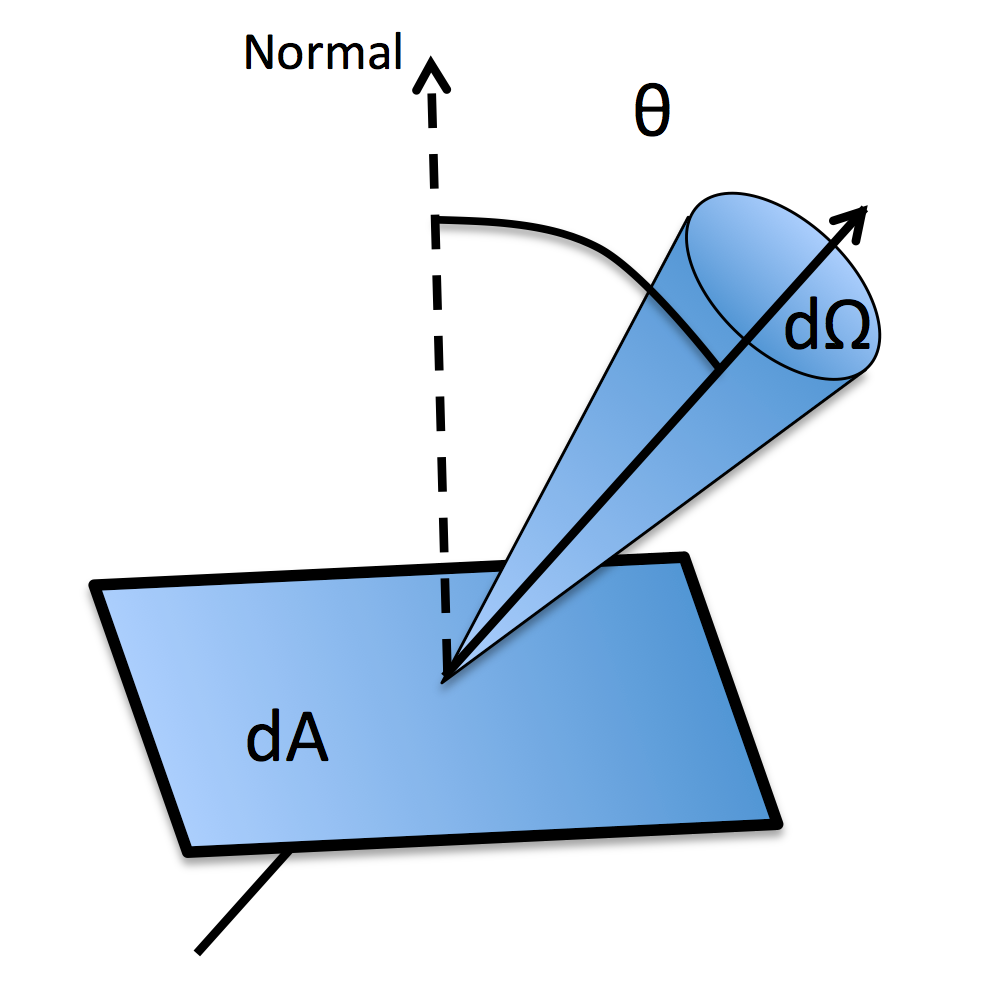
\includegraphics[width=0.5\textwidth]{figures/03-radtrans/rays_schematic.png}
\caption
{
A schematic showing a ray obliquely incident on a surface of area $dA$.
The labeled quantities are used in the definition of specific intensity.
} 
\label{fig:ray}
\end{figure}


The most fundamental quantity of radiative transfer is the 
{\em specific intensity}, $I_\nu$, defined as

\begin{equation}
I_\nu = \frac{dE}{d\Omega~dt~dA~d\nu},
\end{equation}

which has units of ${\rm erg~s^{-1}~Hz^{-1}~sr^{-1}~cm^{-2}}$.
By successively multiplying by $\cos \theta$ and integrating over solid angle we 
can obtain the first and second `moments' of the radiation field. These
are the flux, $F_\nu$ and momentum flux, $p_\nu$, respectively, given by

\begin{equation}
F_\nu = \int I_\nu \cos \theta~d \Omega,
\end{equation}

\begin{equation}
p_\nu = \frac{1}{c} \int I_\nu \cos^2 \theta~d \Omega
\end{equation}

We can also define the {\em mean intensity}, $J_\nu$, as

\begin{equation}
J_\nu = \frac{1}{4 \pi} \int I_\nu~d \Omega
\end{equation}

The mean intensity is particularly
useful when one wants to ignore the solid angle dependence of the radiation,
for example when considering the impact of an ionizing radiation field.

The equation describing the specific intensity change along a path element $ds$
is the radiative transfer equation, 

\begin{equation}
\frac{d I_\nu}{ds} = -\kappa_\nu I_\nu + j_\nu, 
\end{equation}

where $\kappa_\nu$ and $j_\nu$ are the absorption and emission coefficients respectively.
If we define the optical depth $d \tau_\nu = \kappa_\nu ds$ we can recast this as

\begin{equation}
\frac{d I_\nu}{d \tau_\nu} = -I_\nu + S_\nu
\label{eq:formal_rte}
\end{equation}

where $S_\nu=j_\nu/\kappa_\nu$ is the source function. This equation
is called the {\em formal radiative transfer equation}, and can be solved to give 

\begin{equation}
I_\nu = I_{\nu,0}~e^{-\tau_\nu} + \int^{\tau_\nu}_0 S_\nu (\tau^\prime_\nu)~e^{\tau^\prime_\nu-\tau_\nu} d \tau^\prime_\nu.
\label{eq:rte_solution}
\end{equation}

A useful limit is when the source function is constant in the absorbing medium, in which case
the integral can be easily evaluated to give

\begin{equation}
I_\nu = I_{\nu,0}~e^{-\tau_\nu} + S_\nu (1 - e^{-\tau_\nu}).
\label{eq:rte_solution}
\end{equation}

% The mean intensity, $J_\nu$ is a particularly useful quantity when calculation the ionization
% state 

\subsection{Spectral Line Formation}

From the above equations, it is trivial to show how emission and absorption lines form when
the source function is approximately constant.
Say we have a plasma illuminated by a blackbody of temperature $T_0$, such that
$I_{\nu,0} = B_\nu (T_0)$. The plasma layer then has a different temperature, $T$,
such that $S_\nu = B_\nu (T)$ in that medium. By inspecting equation~\ref{eq:rte_solution}
we can see that if we are optically thick within the line, but optically
thin in the continuum, then inside the line the source term is dominant and outside 
the line the first $I_{\nu,0}~e^{-\tau_\nu}$ term dominates. Therefore, if $T > T_0$ we will 
see an emission line, and if $T < T_0$ we will see an absorption line. 
This approach describes line emission in the blackbody limit; for more complicated SED shapes
it is necessary to construct simple model atoms.

\subsection{The Two Level Atom}

The two level atom formalism is well described by Mihalas (1978). 


\subsubsection{Einstein Coefficients}

Within the two level atom, the rate equation between the two levels in LTE can
can be written by invoking detailed balance, such that 
\begin{equation}
B_{lu} \bar{J}_{ul} n_l = B_{ul} \bar{J}_{ul} n_u + A_{ul} n_u,
\label{eq:rate_einstein}
\end{equation}
where $B_{ul}$, $B_{2ul}$ and $A_{ul}$ are the {\em Einstein coefficients}
for absorption, stimulated emission and spontaneous emission respectively.
The `mean intensity in the line', $\bar{J}_{ul}$, is given by
\begin{equation}
\bar{J}_{ul} = \int \phi(\nu) J_\nu d\nu.
\label{eq:jbar}
\end{equation}
In LTE, the level populations obey Boltzmann statistics, and thus we can also
write
\begin{equation}
\frac{n_l}{n_u} = \frac{g_l}{g_u} \exp (h \nu_{ul} / k_B T)
\end{equation}
We can then rearrange equation~\ref{eq:rate_einstein} in terms of the mean intensity,
and use the fact that, in LTE, $\bar{J}_{ul} = B_\nu (T)$ to write
\begin{equation}
\bar{J}_{ul} = (2 h \nu_{ul}^3) / c^2.
\end{equation}
Since this must be true at all values of $T$ we can also show that 
\begin{equation}
A_{ul} / B_{ul} = (2 h \nu_{ul}^3)~B_{lu} / B_{ul} = g_u / g_l
\end{equation}



\subsubsection{Collision Strengths}

As well as radiative excitation and de-excitation, bound electrons 
can also interact with the thermal pool of free electrons, meaning that
collisional rates also affect 




\subsection{The Sobolev Approximation}

The Sobolev approximation (SA) is a useful limit originally developed.
It is used to treat line transfer in fast-moving flows. Originally 
the theory was mostly applied to Stellar winds, although since then
a wide variety of astrophysical objects have been modelled using Sobolev treatments,
such as accreting systems (this work) and Supernovae.

The Sobolev limit is when the local bulk velocity gradients in a flow 
dominate other any thermal broadening. In the presence of these steep
velocity gradients, one can assume that the interaction of a ray with a bound-bound
transition takes place over a small resonant zone, known as a 
`Sobolev surface'. The length of this zone is defined by
\begin{equation}
l_s = \frac{v_{th}}{dv / ds}.
\end{equation}
It is important that the physical conditions of the c do not change on this scale.
If this is the case, then we can assume that all line interactions for a given 
frequency will occur at a single `resonant' point. The location at which
a given photon will interact with a line of frequency $\nu_{lu}$
is then given, in velocity space, by
\begin{equation}
v = c~\left(\frac{\nu}{\nu_{lu}} + 1\right).
\end{equation}
The Sobolev optical depth is then
\begin{equation}
d \tau = \frac{\pi e^2}{m c}  \left(n_l - n_u \frac{g_l}{g_u} \right) \frac{f_{lu} \lambda_{lu}}{c | dv / ds |}.
\end{equation}
We can see that the physical quantities determining line opacity are therefore 
the level populations in the plasma, the velocity gradient and the atomic physics
associated with the bound-bound transition.



\subsubsection{Escape Probabilities}





\subsection{Monte Carlo approaches}

Simple radiation transfer problems can be solved analytically,
but with more complicated geometries it is necessary to use Monte Carlo
techniques, which are easily solved with modern computing approaches and 
are intuitively parallelisable problems. I will describe one specific 
Monte Carlo radiative transfer (MCRT) code, which has been used
for the majority of the work in this thesis.

\section{{\sc python}: A Monte Carlo Ionization and Radiative Transfer Code}
\label{sec:python}

\py\footnote{Named c. 1995, predating the inexorable rise of a certain widely used
programming language.} is a confusingly named 
Monte Carlo ionization and radiative transfer code. 
The general philosophy of the code is to be able to produce synthetic spectra
for astrophysical objects with outflows in 2.5D, using a self-consistent ionization 
treatment. The code is written in C, and has been in development since the mid-1990s.
Throughout this time it has been used with application to CVs \citep{LK02, M15},
YSOs \citep{simmacro2005}, Supernovae \citep{kerzendorfsim} and AGN/quasars 
\citep{higginbottom2013,H14,M16}. It is also capable of producing spectra 
for stellar winds and conducting simple photoionization balance calculations for
comparison with codes such as \textsc{cloudy}. Some more detail on code testing and 
development can be found in sections~\ref{sec:code_validation} and \ref{sec:code_maintenance}
respectively. Although the operation of \py\ is well-described by the above authors,
it is central to this Thesis and I will thus provide substantial detail on its operation. 

\subsection{Basics}

\begin{figure}
\centering
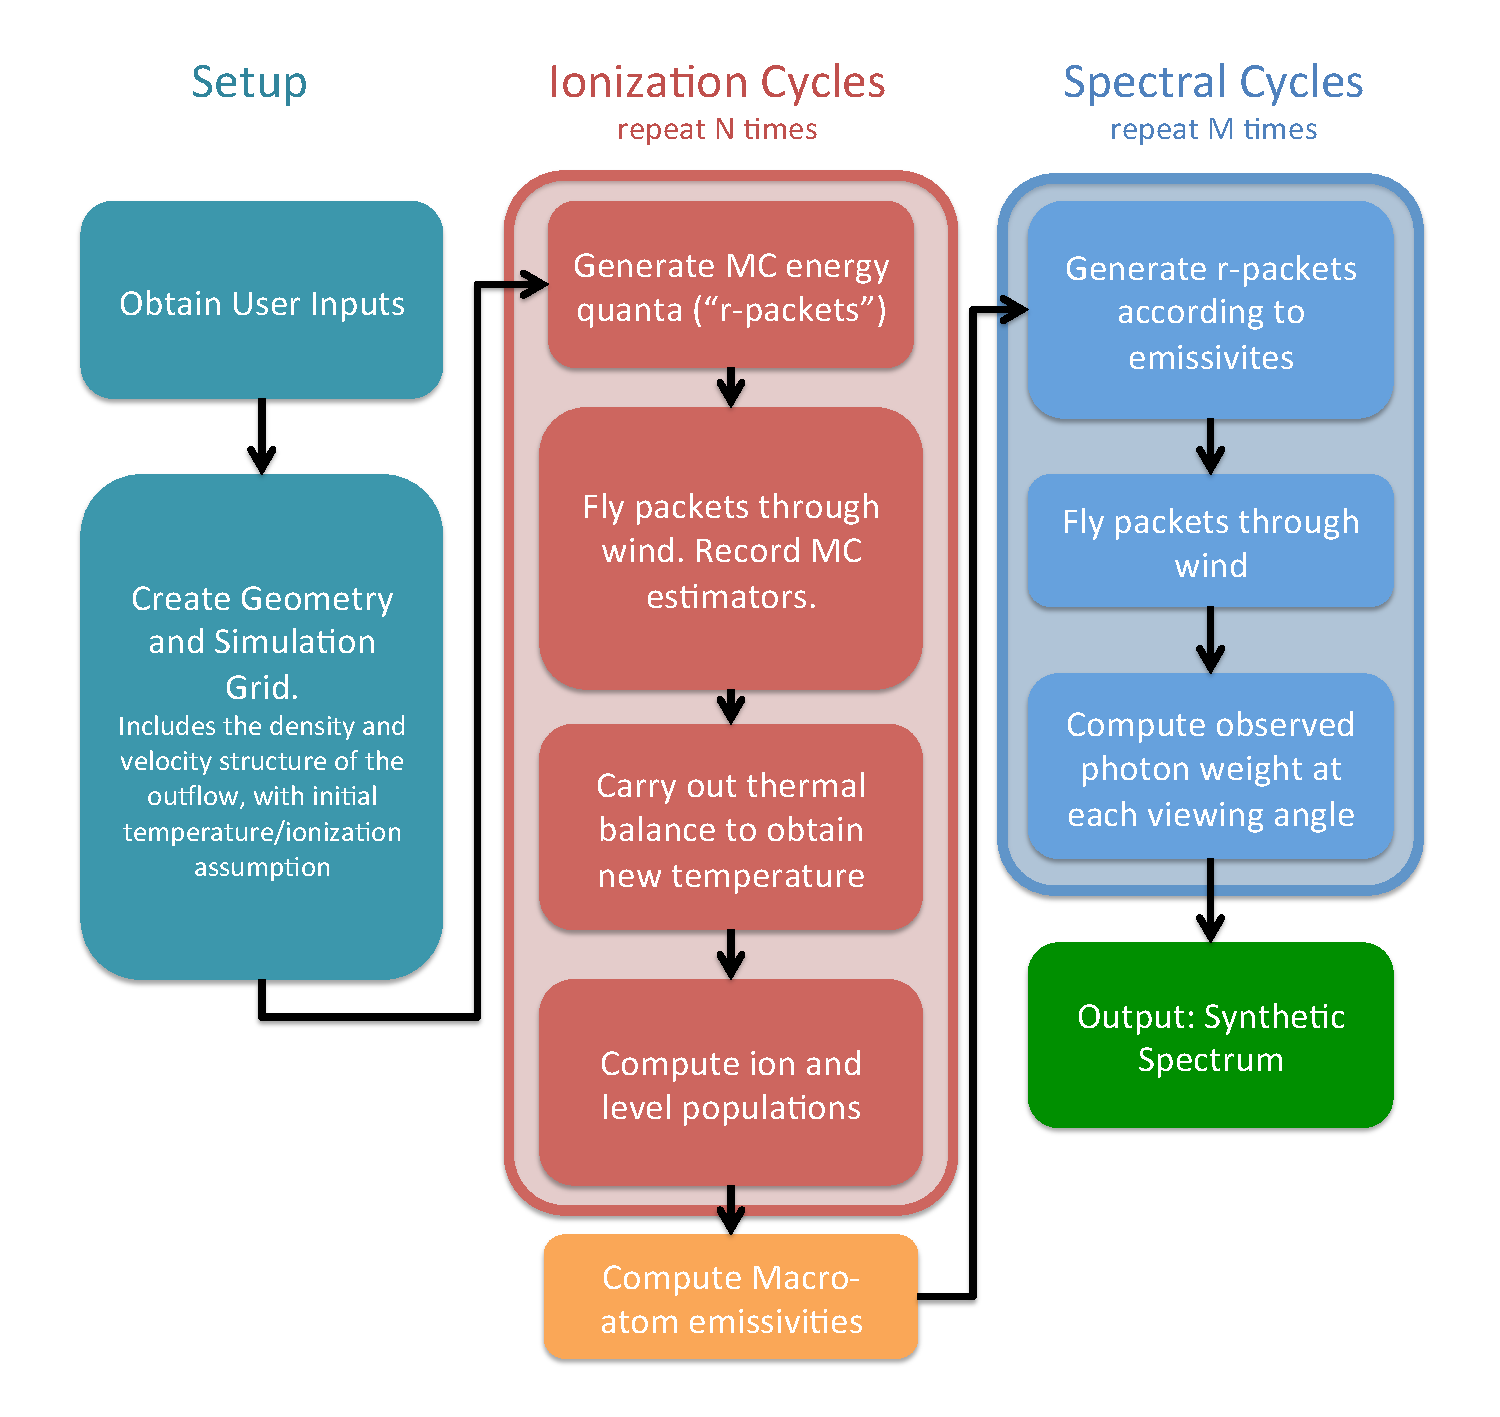
\includegraphics[width=1.0\textwidth]{figures/03-radtrans/flowchart.pdf}
\caption
{
A flowchart showing the basic operation of \py.
} 
\label{fig:flowchart}
\end{figure}

\py\ operates in three distinct stages, shown in figure~\ref{fig:flowchart}. 
First, the user specifies the photon sources,
geometry and kinematics of the system, normally with a similar parameterisation
to the SV93 model described in section~\ref{sec:sv93_model}. 
The code can operate with multiple coordinate systems 
(1D, spherical polar, cylindrical), but in this work I use cylindrical coordinates.
In this case, the outflow is discretised into a $n_x \times n_y$ logarithmic grid with 
user-specified dimensions. The co-ordinates, $(x_i, z_i$), 
of the corner of the $i$th cell are then given by
\begin{equation}
x_i = L_{x}~10^{(i-1)\frac{\log (R_{max} / L_{x})}{n_x}};~~
z_i = L_{z}~10^{(i-1)\frac{\log (R_{max} / L_{z})}{n_z}}, \\
\end{equation}
where $L_x$ and $L_z$ are appropriately chosen (but hardwired) scale lengths.
From these co-ordinates the poloidal distance can be calculated and
the velocity set according to equation~\ref{eq:v_law}. The density
is then calculated by imposing conservation of mass.

Once the basic setup process has been carried out, the ionization state,
level populations and temperature structure are calculated.
This is done via an iterative process, by transporting several populations of 
Monte Carlo energy quanta (`photons' or `$r$-packets) through the outflow.
This process is repeated until the code converges. 
In each of these iterations (`ionization cycles'), the code records estimators that 
characterize the radiation field in each grid cell. At the end 
of each ionization cycle, a new electron temperature is calculated
that more closely balances heating and cooling in the 
plasma. The radiative estimators and updated electron
temperature are then used to revise the ionization state of the wind,
and a new ionization cycle is started. The process is repeated until
heating and cooling are balanced throughout the wind. 

This converged model as the basis for the second set of
iterations (`spectral cycles'), in order to compute the synthetic spectrum based on the 
MC estimators record during the ionization cycles. 
The emergent spectrum over the desired spectral range is synthesized by 
tracking populations of energy packets through the wind and computing the emergent spectra at
a number of user-specified viewing angles.  

\py\ is designed to operate in a number of different
regimes, both in terms of the scale of the system and in terms of the
characteristics of the underlying radiation field.
It was originally developed by LK02 in order to model the UV spectra
of CVs with a simple biconical disc wind model. SDL05
\nocite{simmacro2005} used the code to model Brackett
and Pfund line profiles of H in young-stellar objects (YSOs). As part
of this effort, they implemented a `macro-atom' mode (see below) in
order to correctly treat H recombination lines with
\py. Finally, H13 used \py\ to model broad absorption line (BAL) QSOs. For
this application, an improved treatment of ionization was implemented,
so that the code is now capable of dealing with arbitrary
photo-ionizing SEDs, including non-thermal and multi-component ones. 


\section{Macro-atoms}

{\sl The macro-atom scheme was created by Leon Lucy and is outlined in 
his 2002/03 papers. It was implemented in \py\ by Stuart Sim, initially
for the study of recombination lines in YSO (Sim et al. 2005).}

Lucy (2002, 2003\nocite{lucy2002, lucy2003}; hereafter L02, L03) 
has shown that it is possible to calculate the emissivity of a gas in
statistical equilibrium without approximation for problems with large departures
from LTE.
% accurately by quantising matter into
% `macro-atoms', and radiant and kinetic energy into indivisible energy
% packets (r- and k- packets, respectively). 
His macro-atom scheme allows for all possible transition paths from a given level,
dispensing with the two-level approximation, and
provides a full non-local-thermodynamic-equilibrium (NLTE) solution
for the level populations based on Monte Carlo estimators. The macro-atom
technique has already been used to model Wolf-Rayet star
winds \citep{sim2004}, AGN disc winds \citep{simlong2008, tatum2012},
supernovae \citep{kromersim2009, kerzendorfsim} and YSOs (SDL05). A full 
description of the approach can be found in L02 and L03. 

The fundamental approach here requires somewhat of a philosophical shift.
Normally MCRT is described in the most intuitive way- that is, we imagine
real photons striking atoms and scattering, or photoionizing 
and depositing energy in a plasma. With Lucy's scheme we should instead 
reimagine the MC quanta as a packets of quantised energy flow, and the scheme as a 
{\em statistical} one. The amount of time a given energy quanta spends in a specific atomic
level or thermal pool is then somewhat analogous to the absolute energy 
contained therein.

Following L02, let us consider an atomic species interacting with a radiation field.
If the quantity $\epsilon_j$ represents the ionization plus excitation energy of 
a level i then the rates at which the level $j$ absorbs and emits radiant energy 
are given by

\begin{equation}
 \dot{A}_{j}^{R} = R_{\ell j} \epsilon_{j \ellp} \;\;\;\;\; and \;\;\;
\;\;  \dot{E}_{i}^{R} = R_{j \ellp} \epsilon_{j \ellp} \;\;\; ,
\end{equation}

Where I have adopted Lucy's convention in which the subscript 
$\ellp$ denotes a summation over all lower states.
Similarly, the rates corresponding to {\em kinetic} energy transport can then be written as

\begin{equation}
 \dot{A}_{j}^{C} = C_{\ellp j} \epsilon_{j \ellp} \;\;\;\;\; and
\;\;\;
\;\;  \dot{E}_{j}^{C} = C_{j \ellp} \epsilon_{j \ellp} \;\;\; ,
\end{equation}

If we now impose statistical equilibrium
%
\begin{equation}
 ({\cal R}_{\ellp j}-{\cal R}_{j \ell})+({\cal R}_{uj}-{\cal R}_{ju})=0 \;\;\;.
\end{equation}
 
we can then obtain 

\begin{eqnarray}
 \dot{E}_{j}^{R}+\dot{E}_{j}^{C}+{\cal R}_{ju}\epsilon_{i}+
 {\cal R}_{j \ell}\epsilon_{\ell}  \nonumber \\  
 = \dot{A}_{j}^{R}+\dot{A}_{j}^{C}+{\cal R}_{uj} \epsilon_{i}
 +{\cal R}_{\ell j} \epsilon_{\ell}           .  
 \label{eq:matom_SE}     
\end{eqnarray}

This equation is the starting point for the macro-atom scheme. It shows 
that, when assuming only radiative equilibrium, the energy flows through
a system depend only on the transition probabilities and atomic physics
associated with the levels the energy flow interacts with.
By quantising this energy flow into radiant (r-) and kinetic (k-) packets, 
we can simulate the energy transport through
a plasma discretised into volume elements (``macro-atoms''),
whose associated transition probabilities govern the interaction 
of radiant and kinetic energy with the ionization and excitation energy associated 
with the ions of the plasma.

Although equation~\ref{eq:matom_SE} assumes strict radiative equilbrium,
it is trivial to adjust it to include non-radiative source and sink terms. 
For example, in an expanding parcel of plasma, adiabatic cooling may be 
included with a simple modification to the RHS of equation~\ref{eq:matom_SE}.
%% XXX CHECK THIS.

% \subsection{Superlevels}
% One undesirable aspect of the macro-atom scheme is that the number of 
% jumps made inside a macro-atom can become large in certain limits.
% For example, when the plasma starts to approach LTE conditions
% the energy packets will spend a huge amount of time
% jumping between high up levels in a macro-atom. Fortunately, there
% are a number of fairly elegant solutions here. The first would be simply 
% to keep track of net rates-- if two large rates go in opposite directions
% but have a net difference, then all one needs to do is take account of that net
% difference and set the other rate to zero. This could be implemented in \py\, but
% is not currently. Instead, we adopt a method I shall refer to using the 
% term `superlevels'. 

% Once a cycle has been computed, it is possible to calculate departure coefficients, $D_j$
% for a level $j$, which are defined as

% \begin{equation}
% D_j = \frac{n_j}{n_j^{*,T_e}},
% \end{equation}

% which is simply the ratio of a level's population to it's LTE population at the electron temperature.
% If these coefficients approach unity at all levels above some threshold then these
% levels are said to be part of a superlevel. Any time we jump to a level $j$ inside a superlevel
% we instantly select a new level $k$ with a probability

% \begin{equation}
% P(j,k) = \frac{1}{N} \frac{n_j^{*,T_e}}{g_k} \sum_l P(k,l),
% \end{equation}
 
% where $1/N$ is just a normalisation over the sum of these quantities and $\sum_l P(k,l)$ represents 
% the sum of jumping probabilities to lower levels below the superlevel threshold.
% This formula produces the required jumping and deactivation distributions in the limit of LTE
% without having to actually go through the lengthy process of MC sampling the probability space.
% The speed-up can be huge in certain limits-- some models can undergo $\sim10^8$ jumps before deactivation,
% compared to an average of $\sim2$ in Lucy's original simulations.

\subsection{Macro-Atom Estimators}


\subsubsection{Radiation Field Estimators}

One of the most important estimators is the `mean intensity in the line', $\bar{J}_{lu}$,
which is defined by equation~\ref{eq:jbar}. 


\subsubsection{Heating And Cooling Estimators}

\subsection{Ionization Fractions and Level Populations}




\section{Simple-atoms}

% Prior to SDL05, the relative ionization fractions for all atomic
% species were estimated via the modified Saha equation (Mazzali \&
% Lucy 1993)  
% \begin{equation}
% \frac{n_{j+1} n_e}{n_j} = W [\xi + W(1-\xi)]
% \left(\frac{T_e}{T_R}\right)^{1/2}
% \left(\frac{n_{j+1}n_e}{n_j}\right)^*_{T_R}. \label{ionization}
% \end{equation}
% Here, the `starred' term on the right represents abundances computed with
% the Saha equation at temperature $T_R$, but using partition functions
% from the dilute blackbody approximation. 
% $W$ is an effective dilution factor, $\xi$ is the
% fraction of recombinations going directly to the ground state, and
% $T_R$ and $T_e$ are the radiation and electron temperatures,
% respectively. This simple ionization scheme produces reasonable
% results when the photoionizing SED can be approximated by a dilute
% blackbody. This is the case for high-state CVs. (As noted above, an
% improved, but more complex treatment of ionization that is appropriate
% for more complex SEDs is described in H13.) 

% Similarly, the relative excitation fractions within each ionization
% stage of a given species were estimated via a modified (dilute) Boltzmann
% equation,
% \begin{equation}
% \frac{n_{jk}}{n_j} = \frac{W g_k}{z_j(T_R)} \exp(-E_k/kT_R),
% \end{equation}
% where $n_{jk}$ is the population of level $k$ in ionic stage $j$,
% $E_k$ is the energy difference between level $k$ and the ground state,
% $g_k$ is the statistical weight of level $k$
% and $z_j(T_R)$ is the partition function of ionic stage $j$. 
% This equation is approximate, and in general this approximation 
% is not good. We therefore endeavour to treat any species in
% which the excitation state of the ions is thought to be important
% in determining either the ionizing radiation field, or emergent spectrum,
% as macro-atoms.

% Finally, \py\ originally modelled all bound-bound processes as transitions
% within a simple two-level atom \cite[e.g.][]{mihalas}. 
% This framework was used for the treatment of line transfer and also
% for the line heating and cooling calculations (see LK02). 
% The approximation works reasonably well for resonance  
% lines, such as \civfull, in which the lower level is the ground state.  
% However, it is a poor approximation for many other
% transitions, particularly those where the upper level
% is primarily populated from above. Thus an improved method for
% estimating excited level populations and simulating line transfer is
% needed in order to model recombination lines and continua.

\section{Heating And Cooling}

\subsection{Heating And Cooling Balance}

\subsection{Heating And Cooling Estimators}


Here I've tried to use Lucy's notation for macro-atom estimators. Take a three level system, in
which $l$ and $u$ represent lower and upper levels, 
and $\kappa$ represents the continuum level or upper ion.
q is the `absorption fraction' derived below, and $q_{ul}$ and $q_{lu}$ are the collisional
rate coefficients.

\subsubsection{Macro-atoms}

\noindent
In the macro-atom approach, we basically treat two communication pathways.
bound-free transitions represent a way
for radiant energy to communicate with the thermal pool
and bound-bound transitions represent a way
for excitation energy to communicate with the thermal pool.
\bigskip

\noindent
The heating and cooling rates for macro-atom bound-bound transitions are the rates of
collisional excitations and de-excitations
- i.e. the rate at which thermal energy is converted into
bound-bound excitation energy and vice versa.

\begin{equation}
C_{bb,matoms} = \sum_{lines} q_{lu} n_l n_e h \nu_{ul} V
\end{equation}

\begin{equation}
H_{bb,matoms} = \sum_{lines} q_{ul} n_u n_e h \nu_{ul} V
\end{equation}

\noindent
For bound-free transitions, we define the normal photoionization and recombination
rate coefficients $\gamma$ and $\alpha$, where $\alpha$ includes
stimulated recombination as we do in the code. Note
this differs to the approach in Lucy (2003), where it is instead included as a 
negative photoionization term, hence the notation $\widetilde{\gamma}$.
We also need to define two `modified rate coefficients' which 
are the rates at which b-f transitions add and remove energy to the radiation field.
These are denoted $\gamma^E$ and $\alpha^E$.

The rate at which recombinations convert
thermal {\em and} ionization energy into radiant energy is then
$\alpha^E h\nu_{\kappa l} n_\kappa n_e$, where $h \nu_{\kappa l}$ is the potential of the 
b-f transition, or the energy difference between continuum $\kappa$ and 
the level $l$ we are recombining too. 
The amount of this energy which is removed from the actual thermal pool
therefore needs a quantity $\alpha h\nu_{\kappa l} n_\kappa n_e$ subtracted from it,
giving
\begin{equation}
C_{bf,matoms} = \sum_{bf jumps} (\alpha^E - \alpha) n_e n_{\kappa}\nu_{\kappa l} V 
\end{equation}
where here I have also included stimulated recombination as we do in the code. Note
this differs to the approach in Lucy (2003), where it is instead included as a 
negative photoionization term, hence the notation $\widetilde{\gamma}$.
For photoionizations, we write a similar expression. The rate of at which
a level $l$ absorbs energy by b-f transitions is given by $\gamma^E h\nu_{\kappa l} n_\kappa n_e$,
but the amount $\gamma h \nu_{\kappa l} n_l$ goes into ionization energy, giving 
\begin{equation}
H_{bf,matoms} = \sum_{bf jumps} (\gamma^E - \gamma) n_l h \nu_{\kappa l} V
\end{equation}
as the rate at which radiant energy heats the plasma via b-f transitions.




\subsubsection{Simple-atoms}
\noindent
In simple-ions it is in some ways a little more complicated. 
First we define $q$ which will be different for each b-b transition, 
following Nick's thesis, which is given by 
(NB: I don't actually know how to derive this)
\begin{equation}
q = \frac{q_{ul} n_e (1 - e^{-h\nu/kT_e})}{\beta_{ul} A_{ul} + q_{ul} n_e (1 - e^{-h\nu/kT_e})}
\end{equation}
where $\beta_{ul}$ is the angle-averaged escape probability. 
$q$ represents {\em the probability that an excited bound electron
will collisionally de-excite}.
Our b-b heating rate is computed during the photon propagation and is a sum
over photons which come into resonance with each line, given by 
\begin{equation}
H_{bb,simple} = \sum_{photons} \sum_{lines} (1 - q) (1 - e^{-\tau_S}) w_{photon}
\end{equation}
And our bound bound cooling rate is given by 
\begin{equation}
C_{bb,simple} = \sum_{lines} q \left(n_l\frac{g_u}{g_l} - n_u\right) q_{ul} n_e 
\frac{(1 - e^{-h\nu/kT_e})}{(e^{h\nu/kT_e} - 1)}  h \nu_{ul}
\end{equation}
%%note the difference to the macro-atom approach- here this is already 
\noindent
The bound-free heating rate is given by
\begin{equation}
H_{bf,simple} = \sum_{photons} \sum_{bfjumps} w_{photon} e^{-\tau} \frac{\nu - \nu_{0}}{\nu}
\end{equation}
where $\nu$ here is the frequency of the photon in question, and $\nu_{0}$.
The bound-free cooling rate is then

\begin{equation}
C_{bf,simple} = ??
%%\sum_{bfjumps} \alpha_{sp} n_e n_{\kappa}
\end{equation}













\section{Spectral Synthesis}

The primary output from \py\ is a synthetic spectrum 
across a range of viewing angles. 
The code utilises a variance reduction technique in order to minimise the amount of 
time spent in the portion of the code. This technique is based 
on a similar method implemented by \citep{woods1991}.






A comparison between the two methods is shown in figure~\ref{fig:extract_demo}.

\begin{figure}
\centering
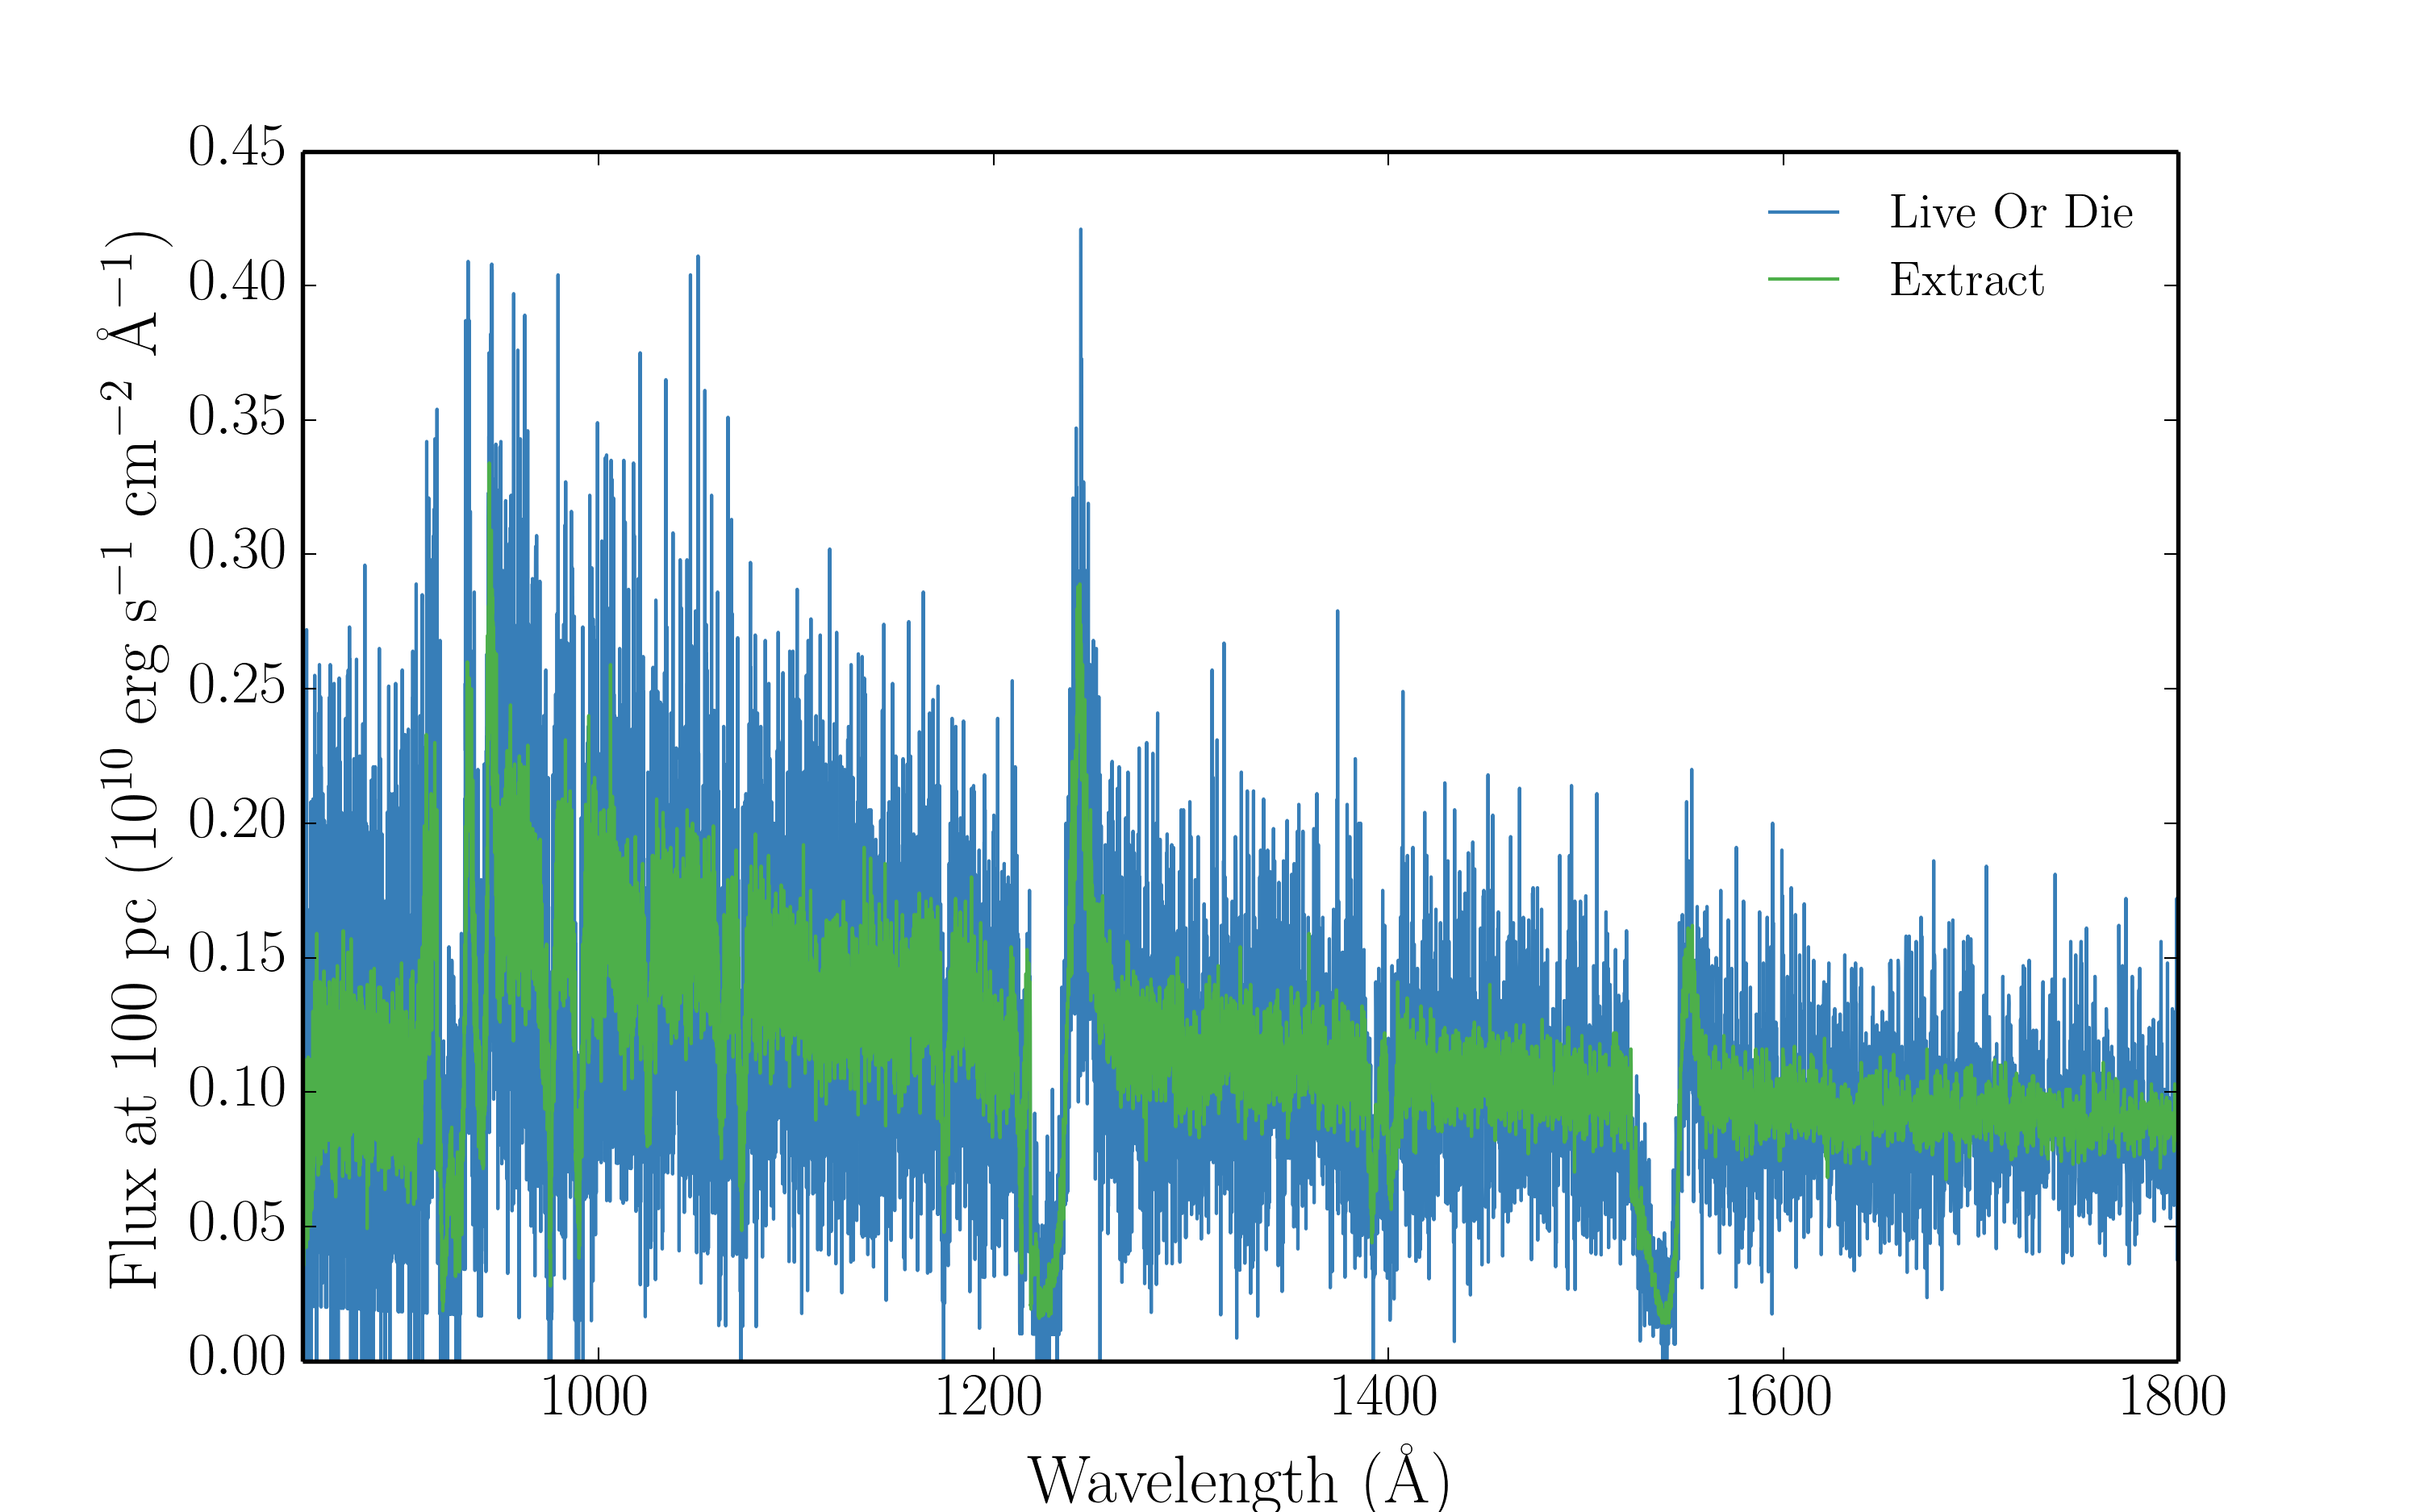
\includegraphics[width=1.0\textwidth]{figures/03-radtrans/extract_demo.png}
\caption
{
A Synthetic spectrum after $30$ spectral cycles with $100,000$ photons
from simple CV wind model at a $60^\circ$ viewing angle.
Spectra produced with both the extract and live or die modes
are shown. The effectiveness of the extract variance reduction technique can
be clearly seen, and we can see that the spectral shape is unaltered.
} 
\label{fig:extract_demo}
\end{figure}




\section{Atomic Data}

One of the big challenges in building reliable photoionization and radiative
transfer lies in the acquisition of accurate and complete atomic datasets.
All of the rates described so far contain a term, such as the oscillator strength 
or dimensionless collision strength, that is dependent purely on the atomic physics
associated with the transition. These quantities can be measured in laboratory experiments,
or predicted from atomic structure codes which derive the atomic physics from 
quantum theory.

Photoionization cross-sections are obtained from two sources. Where possible,
we use \top\ photoionization cross-sections. For macro-atoms,
these cross-sections are partial and represent the cross-section for a photoionization
from a given {\em level}. We neglect photoionizations to excited configurations
of the upper ion. For simple-atoms they are from the ground state.
The \top\ cross-sections have two major drawbacks in that 





\section{Clumping}

\label{sec:microclumping}

\subsection{Motivation}

As described in section~??, observational evidence for inhomogeneities in 
outflows is widespread. Clumping a plasma can have a significant effect on its
ionization, emission and absorption characteristics. Clearly, the interplay between
these effects will be somewhat complex 

A number of different implementations of clumping have been explored in previous studies,
mostly in the stellar winds community. Perhaps the simplest method is 
when one assumes that the individual clumps are both optically and geometrically thin;
this is known as {\em microclumping} \citep[e.g.][]{hamann1998,hilliermiller1999,hamann2008}. 
This technique has been particularly successful in reconciling discrepant mass-loss estimates.
It was found that one would obtain different mass-loss rates depending on whether
they were calculated from (i) UV resonance scattering of continuum photons 
(which scales linearly with density; a `$\rho$-diagnostic') or (ii) recombination 
and free-free emission process (which scale with the square of density; 
`$\rho^2$-diagnostics'). A clumped outflow would have enhanced densities in 
certain regions, and would thus mean that $\rho^2$-diagnostics tend to 
overestimate the total mass-loss rates. Microclumping has helped verify this
hypothesis with radiative transfer modelling (REFs). These clumpy models also
provide better fits to the electron scattering wings of emission lines in stellar
winds \citep{hillier1991}.

The second-generation of stellar wind codes went on step further by addressing the issue
of {\em porosity}; that clumps will have a finite size, and thus gaps between the clumps
may affect the emergent radiation field. This approach is known as {\em macroclumping}.
{\bf Describe macroclumping with references.}

Implementing a treatment of clumping in accretion disc wind models is challenging, for
two main reasons. First, the physical scale lengths and density contrasts 
in disc winds are not well-constrained from observations, especially in AGN.  
Second, there are significant computational difficulties associated with adequately
resolving and realistically modelling a series of small scale, high density
regions with a MCRT code. Given the lack of knowledge about the actual 
type of clumping, we encorporated the simpler microclumping approach into our code.
This is partly because our primary concern was the ionization and 
emission characteristics of the flow, and porosity was a secondary concern.


\subsection{Microclumping}

To take account of clumping in our outflow we adopt a simple parameterization
used in stellar wind modelling. The key assumption here is that typical clump sizes
are much smaller than the typical photon mean free path, and thus the clumps are 
both geometrically and optically thin. This approach is typically 
known as microclumping and allows one to introduce a `filling factor', $f$, which is the 
fraction of the volume of the plasma filled by clumps. We can then introduce the 
`density enhancement', $D$, which is simply 

\begin{equation}
D = \frac{1}{f}
\end{equation}

The densities in the model are then multiplied by this factor. This has the effect 
of enhancing `$\rho^2$' processes such as recombination or collisional excitation,
and 


\section{Code Validation}
\label{sec:code_validation}

The main challenge for high performance scientific computing can be 
elegantly summarised by Ferland's (2002) epitaph, {\sl `Reliability in the face 
of complexity'}. I have already delved into some of the complexity in this case,
so it is important to assess whether the code is also reliable before I present
results. 

\subsection{Testing against Cloudy}



\subsection{Testing against Tardis}


\section{Code Maintenance and Version Control}
\label{sec:code_maintenance}

As part of the expansion of the team working on \py\, I was responsible
for bringing the code under the auspices of a robust version control system.
Thanks to these efforts, the code is now hosted on GitHub at 
\url{https://github.com/agnwinds/python/}. Our team uses a Pull \& Fork model
for collaborative code development, in which major changes are made in a 
forked repository before the developer submits a `Pull request' to the main 
repository. To test the code, we use a combination of Travis CI build tests 
-- run per commit to the upstream repo -- and our own test suite which is 
run every night on a multi-core server. 

\begin{figure}
\centering
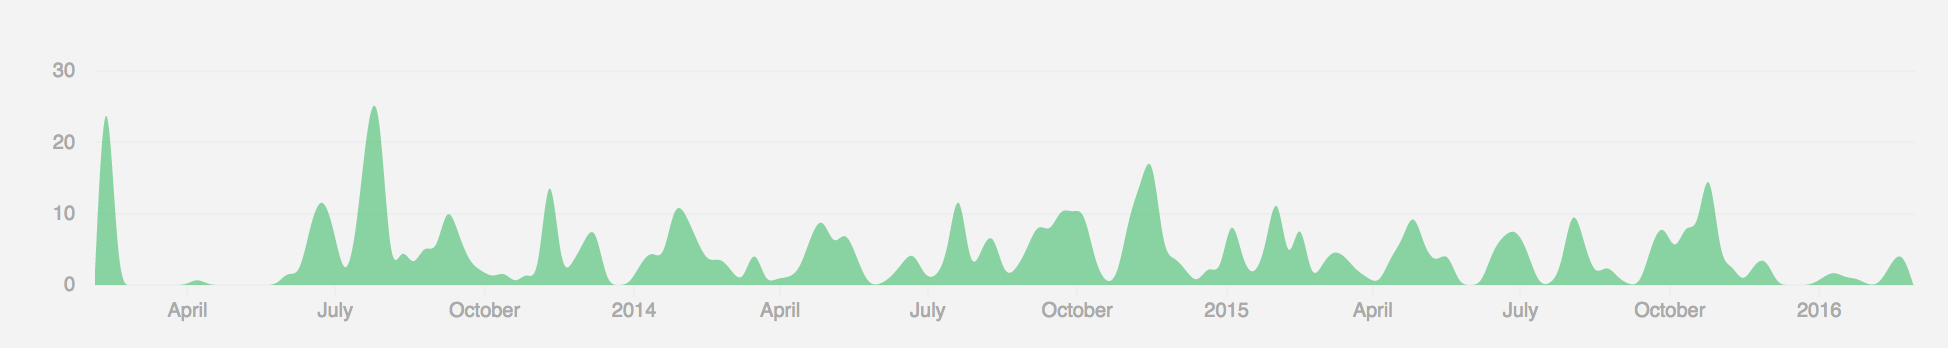
\includegraphics[width=1.0\textwidth]{figures/03-radtrans/github1.png}
\caption
{
Commit history from Feb 3, 2013 to Feb 29, 2016, showing the regular code development
that makes version control such a necessity to a collaborative code project. Produced
using the Github API and plotting capability.
} 
\label{fig:github}
\end{figure}

\subsection{Parallelisation} 










 % Experimental Setup

% % \clearpage

% % \pagestyle{empty}  % Return the page headers back to the "fancy" style

\begin{center}
{\huge {\bf PAPERS}}
\end{center}

\bigskip

The next three chapters consist of the three papers, which constitute the
main science body of this work. They are, in chronological order:

\bigskip
{\bf Chapter 4:} \\
{\sl ``The impact of accretion disc winds on the optical spectra of cataclysmic variables''}\\ 
James~H.~Matthews, Christian~Knigge, Knox~S.~Long, Stuart~A.~Sim, 
and Nick~Higginbottom, Published in 
{\sl Monthly Notices of the Royal Astronomical Society, Volume 450, Issue 3, p.3331-3344.}

\bigskip
{\bf Chapter 5:} \\
{\sl ``Testing quasar unification: clumpy winds and radiative transfer''} \\
James~H.~Matthews, Christian~Knigge, Knox~S.~Long, Stuart~A.~Sim, 
Nick~Higginbottom and Sam~W.~Mangham, Published in 
{\sl Monthly Notices of the Royal Astronomical Society, DOI: 10.1093/mnras/stw323.}


\bigskip
{\bf Chapter 6:} \\
{\sl ``Testing Quasar Unification II.: Orientation Effects and Emission Line Properties''}\\
James~H.~Matthews, Christian~Knigge, to be submitted to
{\sl Monthly Notices of the Royal Astronomical Society.}

\bigskip
I can confirm, in accordance with the `three-paper PhD' guidelines, that as lead author
I have lead the research contained within these papers, including producing all figures and
writing the text. The reader will however notice a change of pronouns due to the 
collaborative nature of the work, and as each paper has a separate introduction there is
also some repetition of background material.

\clearpage % Experimental Setup

% \pagestyle{fancy}  % Return the page headers back to the "fancy" style


% %%%%%%%%%%%%%%%%%%%%%%%%%%%%%%%%%%%%%%
%
%          TITLE AND AUTHORS
%
%%%%%%%%%%%%%%%%%%%%%%%%%%%%%%%%%%%%%%%


\chapter{The Impact of Accretion Disc Winds on the Optical Spectra of Cataclysmic Variables}

{\em This chapter is based on the publication:

Matthews J. H., Knigge C., Long K. S., Sim S. A., Higginbottom N., 
`The impact of accretion disc winds on the optical spectra of 
cataclysmic variables',
2015, MNRAS, 450, 3331.}
%%%%%%%%%%%%%%%%%%%%%%%%%%%%%%%%%%%%%%
%
%          INTRODUCTION
%
%%%%%%%%%%%%%%%%%%%%%%%%%%%%%%%%%%%%%%%

\section{Introduction} 
\label{sec:intro} 

\nocite{groot2004}
\nocite{beuermann1990}
\nocite{beuermann1992}
\nocite{higginbottom2013}

\index{Monte Carlo radiative transfer}
Here, I present Monte Carlo radiative transfer simulations designed
to assess the likely impact of accretion disc winds on the
optical spectra of high-state CVs. The goal is to
test whether the disc winds that produce the UV
resonance absorption lines also naturally create significant amounts of  
optical emission. More specifically, I aim to investigate whether a 
disc wind model can reproduce the optical lines observed in CV spectra,
such as \ha, \hb, \heiiopt\ and the He~\textsc{i} lines, as well as
the \heiiuv\ emission line. I also aim to explore whether the recombination
continuum from the wind can sucessfully `fill-in' the Balmer photoabsorption
edge intrinsic to stellar or disc atmosphere spectra and to establish
if a disc wind model can produce single-peaked lines as proposed
by \citet[][hereafter referred to collectively as MC96]{MC96,MC97}.
The relevant background to this study is outlined in section~\ref{sec:cv_winds}.
\index{cataclysmic variable}\index{disc wind}

In order to carry out these simulations and effectively model the optical
spectra of CVs, I use the `macro-atom' approach described in chapter 3. 
With this method, \py\ is able to deal correctly with processes involving
excited levels, such as the recombination emission observed in CV spectra.
The prescription used to describe the wind is the biconical SV93 model described in 
section~\ref{sec:sv93_model}; a schematic for this specific application
is shown in Fig.~\ref{cartoon}. 
The remainder of this chapter is organized as follows. I begin
by describing the photon sources and input SED used in this modelling.
In section~\ref{modela}, I present spectra simulated from the benchmark 
model employed by LK02. In section~\ref{sec:modelb}, I present a revised model
optimized for the optical waveband, before summarising the
findings in section~\ref{sec:cv_conclusions}.


\subsection{Sources and Sinks of Radiation}
\label{radsources}

\begin{figure} 
\centering
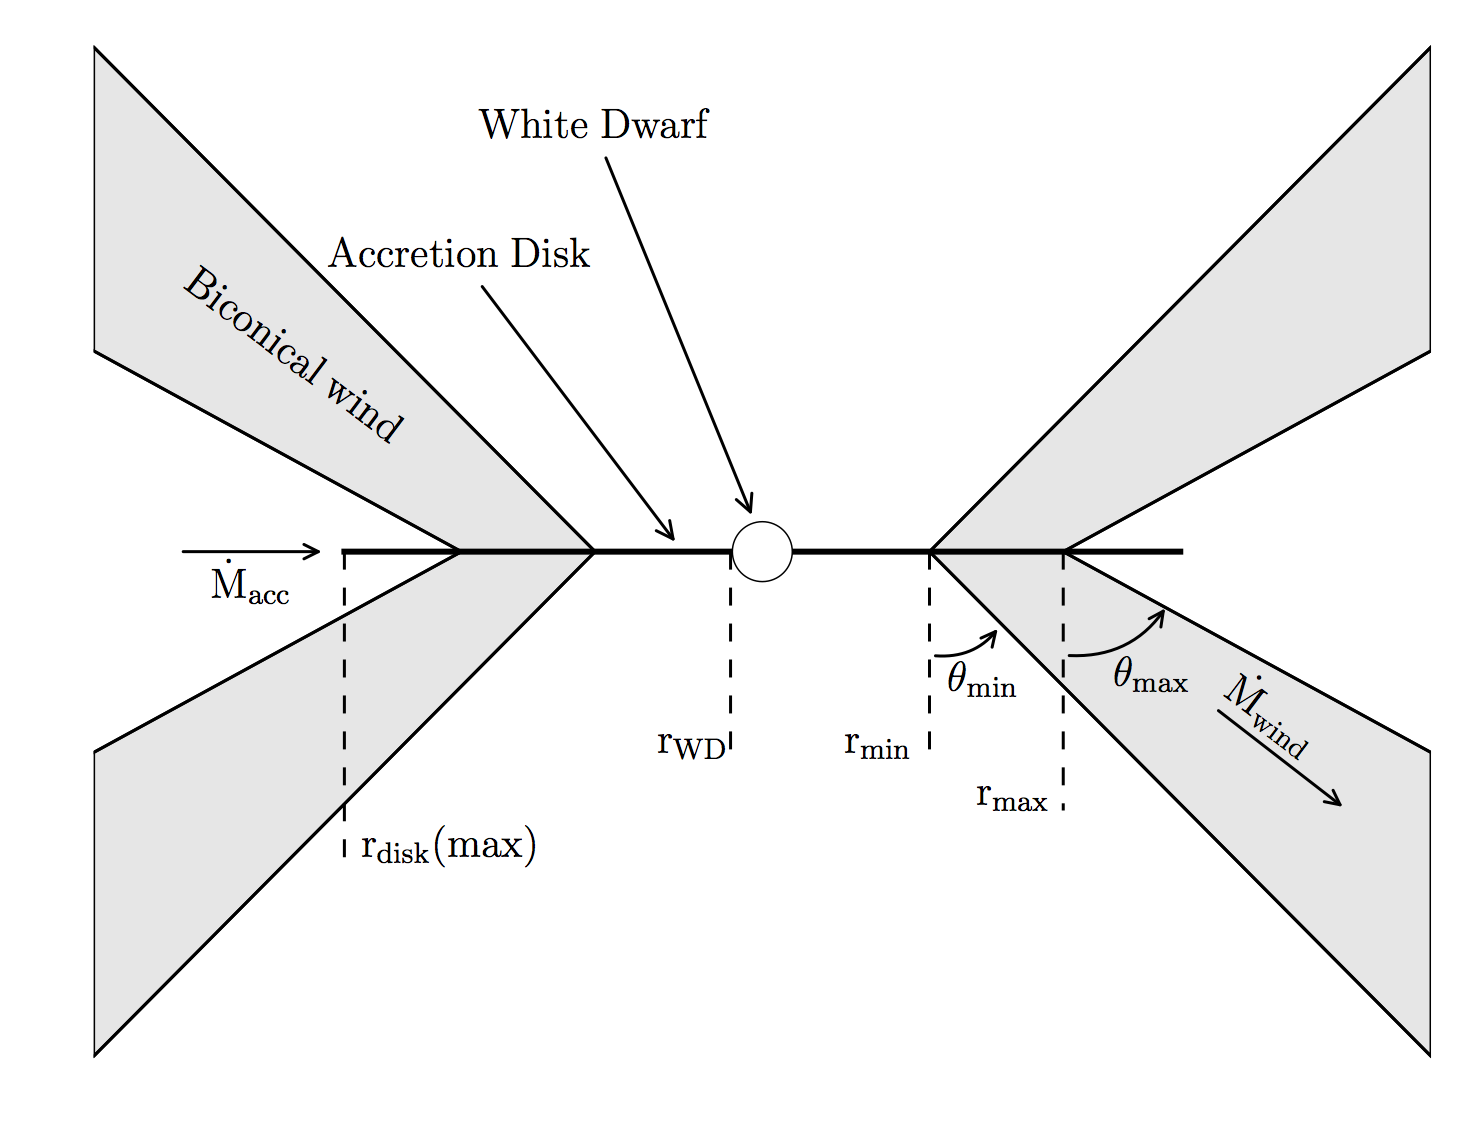
\includegraphics[width=1.0\textwidth]{figures/05-cvpaper/fig2_cartoon.png}
\caption{Cartoon illustrating the geometry and kinematics of the benchmark CV wind model.}
\label{cartoon}
\end{figure} 

The net photon sources in this CV model are the accretion disc, the
WD and, in principle, a boundary layer with user-defined temperature
and luminosity. All of these radiating bodies are taken to be
optically thick, and photons striking them are assumed to be destroyed
instantaneously. The secondary star is not included as a radiation
source, but is included as an occulting body. This allows eclipses to be
modelled. Finally, emission from the wind itself is also accounted for, but
note that this assumes the outflow is in radiative equilibrium. Thus all
of the heating of the wind, as well as its emission, is ultimately
powered by the radiation field of the net photon sources in the
simulation. In the following sections, I will describe the treatment
of these system components in slightly more detail, which are also
shown in Fig.~\ref{cartoon}.

\subsubsection{Accretion disc}

\index{accretion disc}\index{accretion disc!thin disc models}
\index{blackbody}\index{stellar atmosphere}
\py\ has some flexibility when treating the accretion 
disc as a source of photons. The disc is broken down into annuli 
such that each annulus contributes an equal amount to the bolometric
luminosity. The disc is geometrically thin, but optically
thick, and I thus adopt the temperature profile of a standard
\cite{shakurasunyaev1973} $\alpha$-disc. An annulus can then
be treated either as a blackbody with the corresponding effective
temperature or as a stellar atmosphere model with the appropriate
surface gravity and effective temperature. Here, blackbodies are used
during the ionization cycles and to compute the Monte Carlo
estimators. The input SED for the ionization cycles is shown in 
Fig.~\ref{cv_model_sed}.
However, during the spectral synthesis stage of the 
simulation stellar atmosphere models are used. This produces more
realistic model spectra and allows a test of whether recombination
emission from the wind base can fill in the Balmer jump, which is
always in absorption in these models. 
The synthetic stellar atmosphere spectra are calculated with
\textsc{Synspec}\footnote{http://nova.astro.umd.edu/Synspec43/synspec.html}
from either Kurucz \citep{kurucz1991} atmospheres (for $T_{\mathrm{eff}} \leq
50,000$~K) or from \textsc{TLUSTY} \citep{tlusty} models (for $T_{\mathrm{eff}} > 50,000$~K). 
\index{accretion disc}\index{stellar atmosphere}\index{\textsc{TLUSTY}}
\index{Balmer edge}

\begin{figure} 
\centering
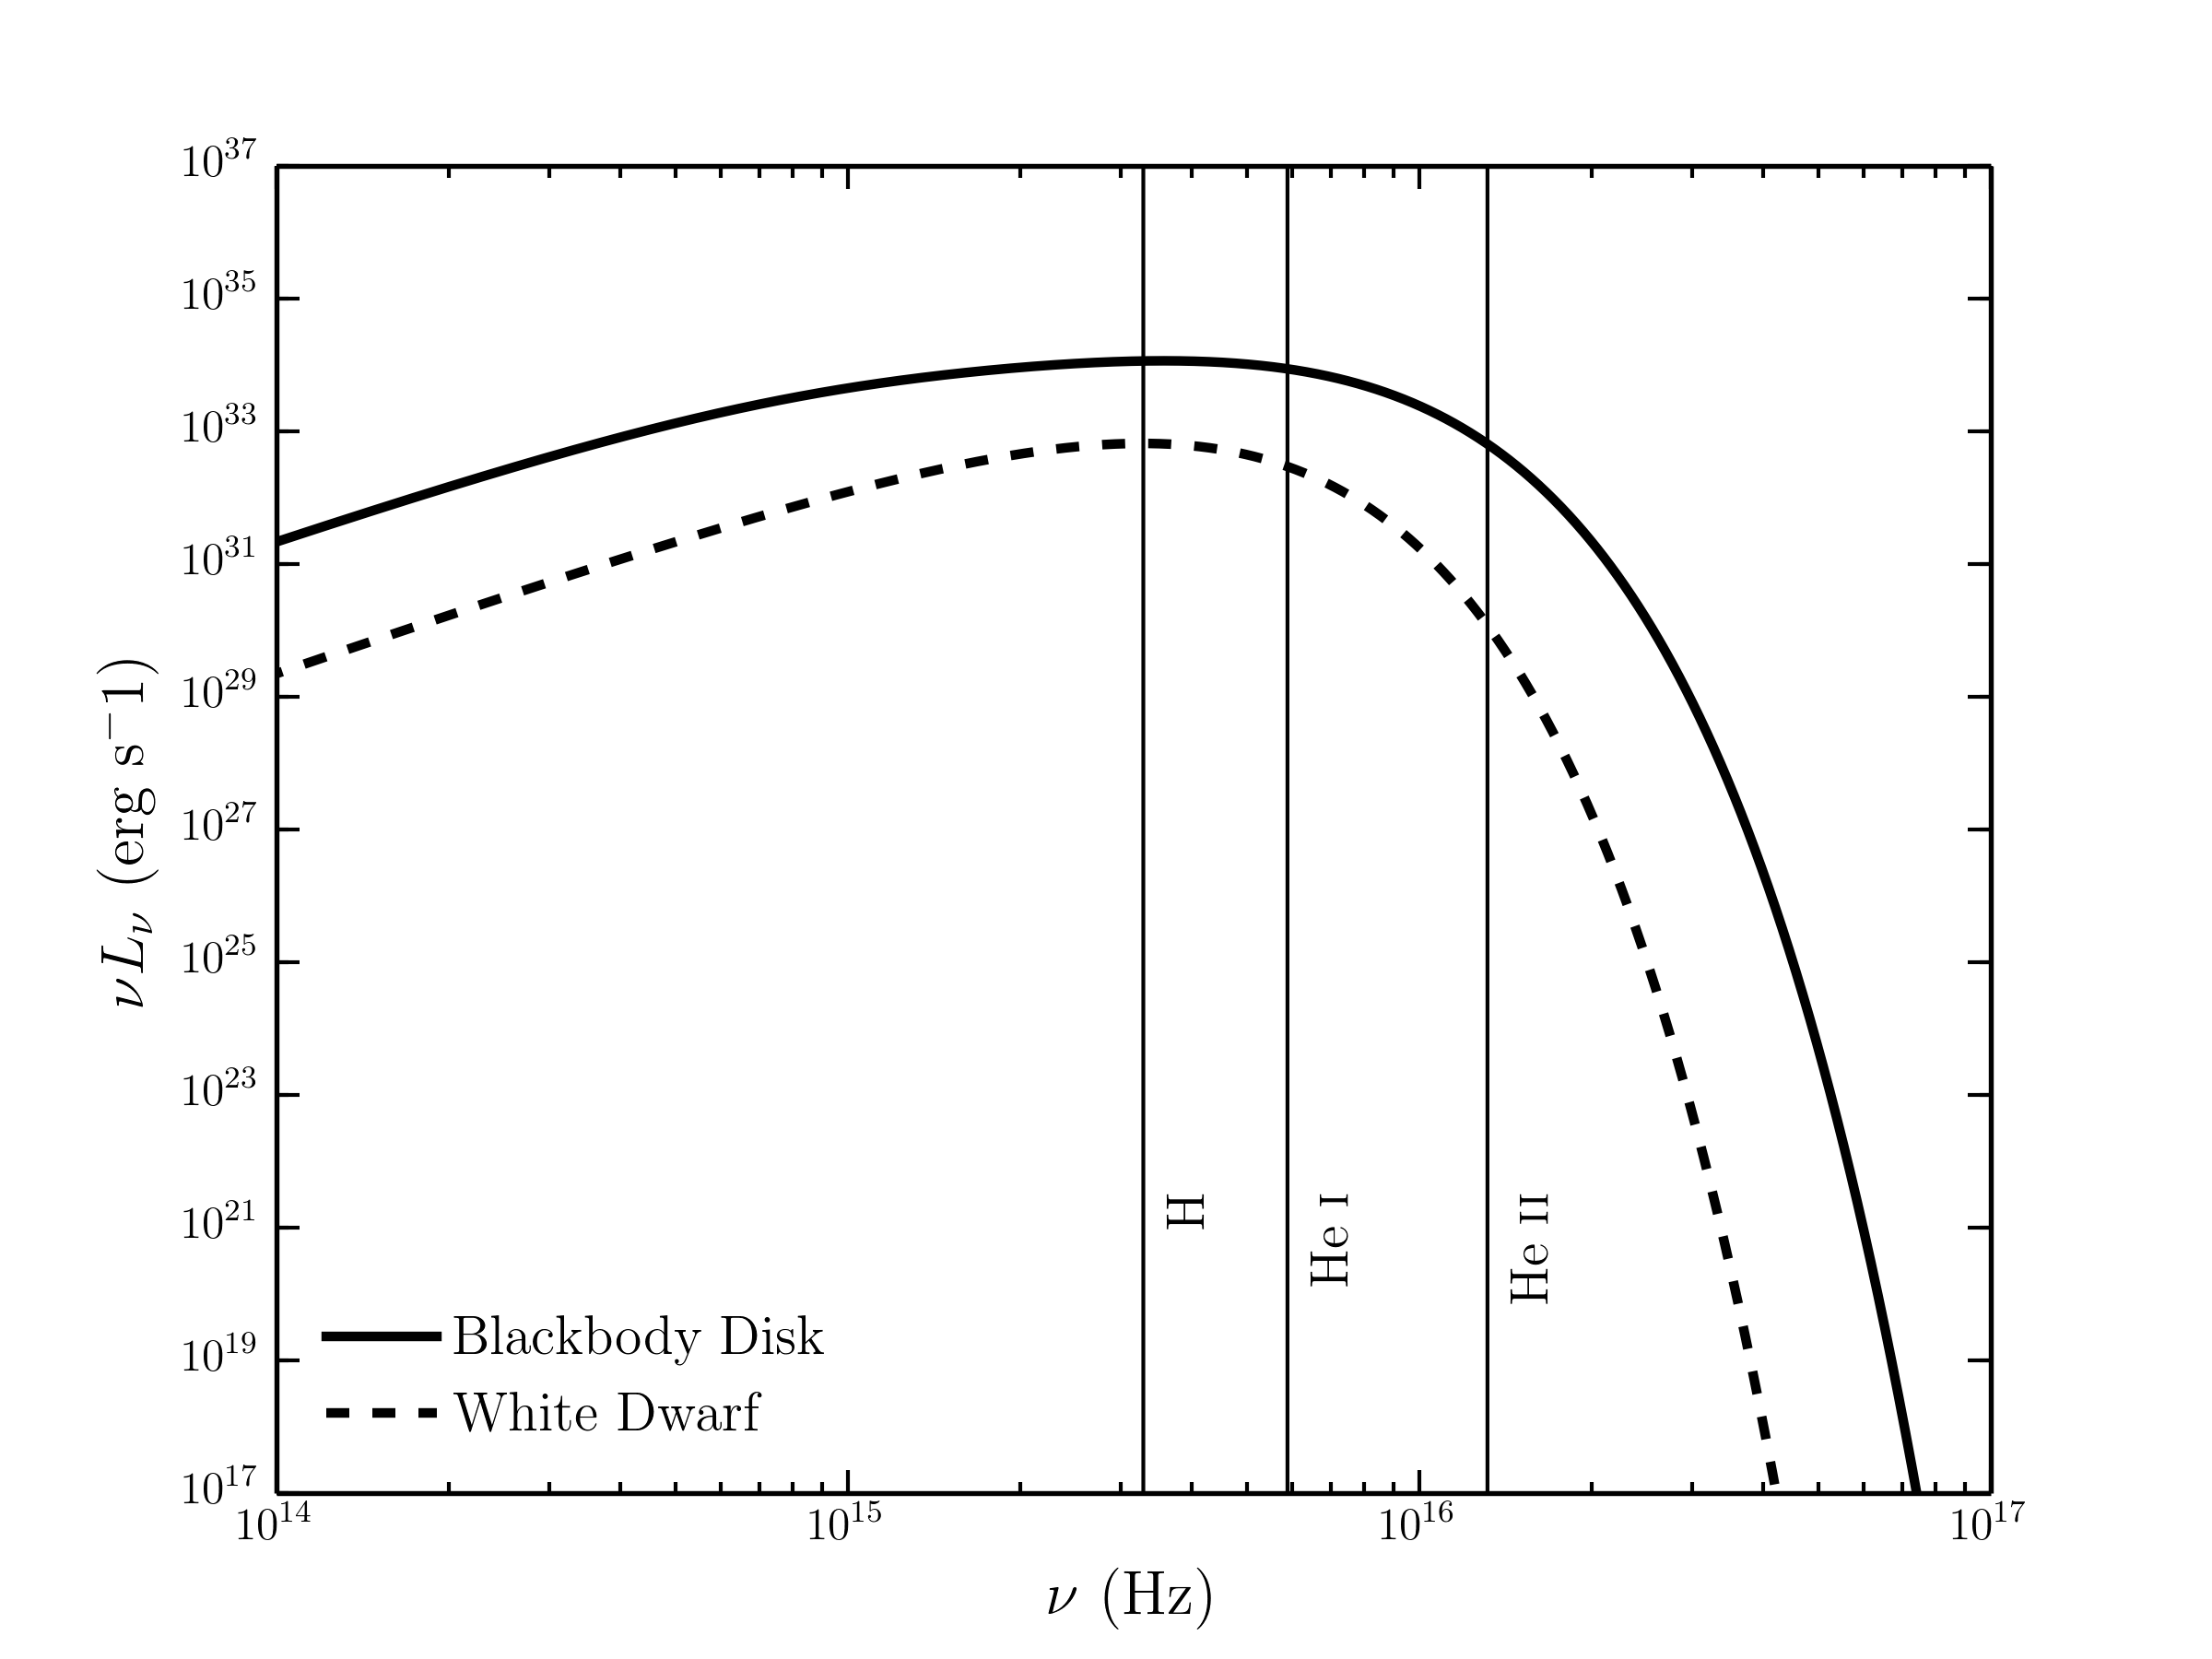
\includegraphics[width=0.8\textwidth]{figures/05-cvpaper/sed.png}
\caption[The spectral energy distribution of the 
accretion disc and white dwarf used in the ionization cycles for
the CV modelling.]{The spectral energy distribution of the 
accretion disc and white dwarf used in the ionization cycles for
the CV modelling. The important ionization edges for
hydrogen and helium are marked.}
\label{cv_model_sed}
\end{figure} 

\subsubsection{White Dwarf}

The WD at the center of the disc is always present as a spherical occulting
body with radius $R_{WD}$ in \py\ CV models, but it can also be included
as a source of radiation. In the models presented here,the
WD is treated as a blackbody radiator with temperature $T_{WD}$ and luminosity
$L_{WD} = 4\pi R_{WD}^2 \sigma T_{WD}^4$.\index{white dwarf}
\index{blackbody}

\subsubsection{Boundary Layer}

It is possible to include radiation from a boundary layer (BL) between
the disc and the WD. In \py, the BL is described as
a blackbody with a user-specified effective temperature and
luminosity. The models presented here initially follow LK02 in setting
the BL luminosity to zero, partly as the temperature, luminosity, and even
existence of a BL in CVs with strong winds is not certain \citep{hoaredrew1993}.
However, I have confirmed that the addition 
of an isotropic BL with $L_{BL} = 0.5 L_{\mathrm{acc}}$ and temperatures in 
the range $80~{\rm kK} \leq T_{BL} \leq 200~{\rm kK}$ would not change 
any of the main conclusions here. 
The influence of the BL on the heating and cooling balance
in the wind, as well as the emergent spectrum, is briefly discussed in
section~\ref{sec:coll_bl}.
\index{boundary layer}\index{blackbody}


\subsubsection{Secondary Star}

The donor star is included in the system as a pure radiation sink, 
i.e. it does not emit photons, but absorbs any photons that strike its
surface. The secondary is assumed to be Roche-lobe filling, so its
shape and relative size are defined by setting the mass ratio of the system, 
$q_M = M_2/M_{WD}$. The inclusion of the donor star as an occulting body
allows eclipses of the disc and the wind to be modelled. For this
purpose, I assume a circular orbit with a semi-major axis $a$ and 
specify orbital phase such that $\Phi_{\mathrm{orb}} = 0$ is the
inferior conjunction of the secondary (i.e. mid-eclipse for $i \simeq
90^\circ$).\index{Roche-lobe}




%%%%%%%%%%%%%%%%%%%%%%%%%%%%%%%%%%%%%%
%
%          BENCHMARK MODEL
%
%%%%%%%%%%%%%%%%%%%%%%%%%%%%%%%%%%%%%%%


\begin{table}
\centering
\begin{tabular}{p{2cm}p{2cm}p{2cm}}
%\multicolumn{2}{l}{Model Parameters}  \\
%%Model Parameters \\
\hline Parameter 	&	 Model A  & Model B \\ 
\hline \hline 
$M_{WD}$ 	 &	 $0.8~M_{\odot}$  &     \\ 
$R_{WD}$ 	 &	 $7\times10^{8}$~cm  & \\ 
$T_{WD}$ 	 &	 $40,000$~K        &  \\
$M_{2}$ 	& -&	 $0.6~M_{\odot}$   \\ 
$q_M$ 	&- &	 $0.75$   \\ 
$P_{\mathrm{orb}}$ 	&- &	 $5.57$~hr   \\ 
$a$ 	& -&	 $194.4~R_{WD}$   \\ 
$R_2$   &   -  &	 $69.0~R_{WD}$  \\ 
$\dot{M}_{\mathrm{acc}}$ 	 &	 $10^{-8}~M_{\odot}\mathrm{yr}^{-1}$  &\\ 
$\dot{M}_W$  &	$10^{-9}~M_{\odot}\mathrm{yr}^{-1}$å  & \\ 
$r_{\mathrm{min}}$ 	&	 $4~R_{WD}$ &  \\ 
$r_{\mathrm{max}}$ 	&	 $12~R_{WD}$  &  \\ 
$r_{\mathrm{disc}}$(max) 	&	 $34.3~R_{WD}$  &  \\ 
$\theta_{\mathrm{min}}$	&	 $20.0^{\circ}$  &  \\ 
$\theta_{\mathrm{max}}$ 	&	 $65.0^{\circ}$  &  \\ 
$\gamma$ 	&	 $1$  &  \\ 
$v_{\infty}$ 	&	 $3~v_{\mathrm{esc}}$  &  \\ 
$R_v$ 	        &	 $7\times10^{10}~\mathrm{cm}$  &  $10^{11}~\mathrm{cm}$  \\ 
$R_v / R_{WD}$ 	&	 $100$  &  $142.9$  \\ 
$\alpha$ 	&	 $1.5$   &   $4$\\
\hline 
\end{tabular} 
\centering
\caption
[Model parameters for the CV wind models]
{
Parameters used for the geometry and kinematics of the benchmark 
CV model (model A), which is optimized for the UV band, and a model
which is optimized for the optical band and described in section~\ref{sec:modelb} (model B).
For model B, only parameters which are altered are given - otherwise the
model A parameter is used. $P_{\mathrm{orb}}$ is the orbital period 
(the value for RW Tri from Walker 1963 is adopted, see section~\ref{sec:rwtri}) and 
$R_2$ is the radius of a sphere with the volume of the secondary's Roche lobe. 
Other quantities are defined in the text or Fig.~\ref{cartoon}.
Secondary star parameters are only quoted for 
model B as I do not show eclipses with the 
benchmark model (see section~\ref{sec:rwtri}).
}
\label{wind_param}
\label{modelb_table}
\end{table}

\nocite{walker1963}

\section{A Benchmark Disc Wind Model}
\label{modela}

\index{disc wind}\index{cataclysmic variable}
The main goal is to test whether the type of disc wind model that has
been successful in explaining the UV spectra of CVs could also have a
significant impact on the optical continuum and emission line spectra
of these systems. In order to set a benchmark, I therefore begin by
investigating one of the fiducial CV wind models that was used by SV93
and LK02 to simulate the UV spectrum of a typical high-state
system. The specific parameters for this model (model A) are listed in
table~\ref{modelb_table}. A key point is that the wind mass-loss rate in this model is
set to 10$\%$ of the accretion rate through the disc. I follow SV93
in setting the inner edge of the wind ($r_{\mathrm{min}}$) to $4~R_{WD}$. 
The sensitivity to some of these parameters is briefly discussed in
section~\ref{sec:cv_params}. 

\subsection{Physical Structure and Ionization State}
\label{modela_ionization}

\begin{figure*}
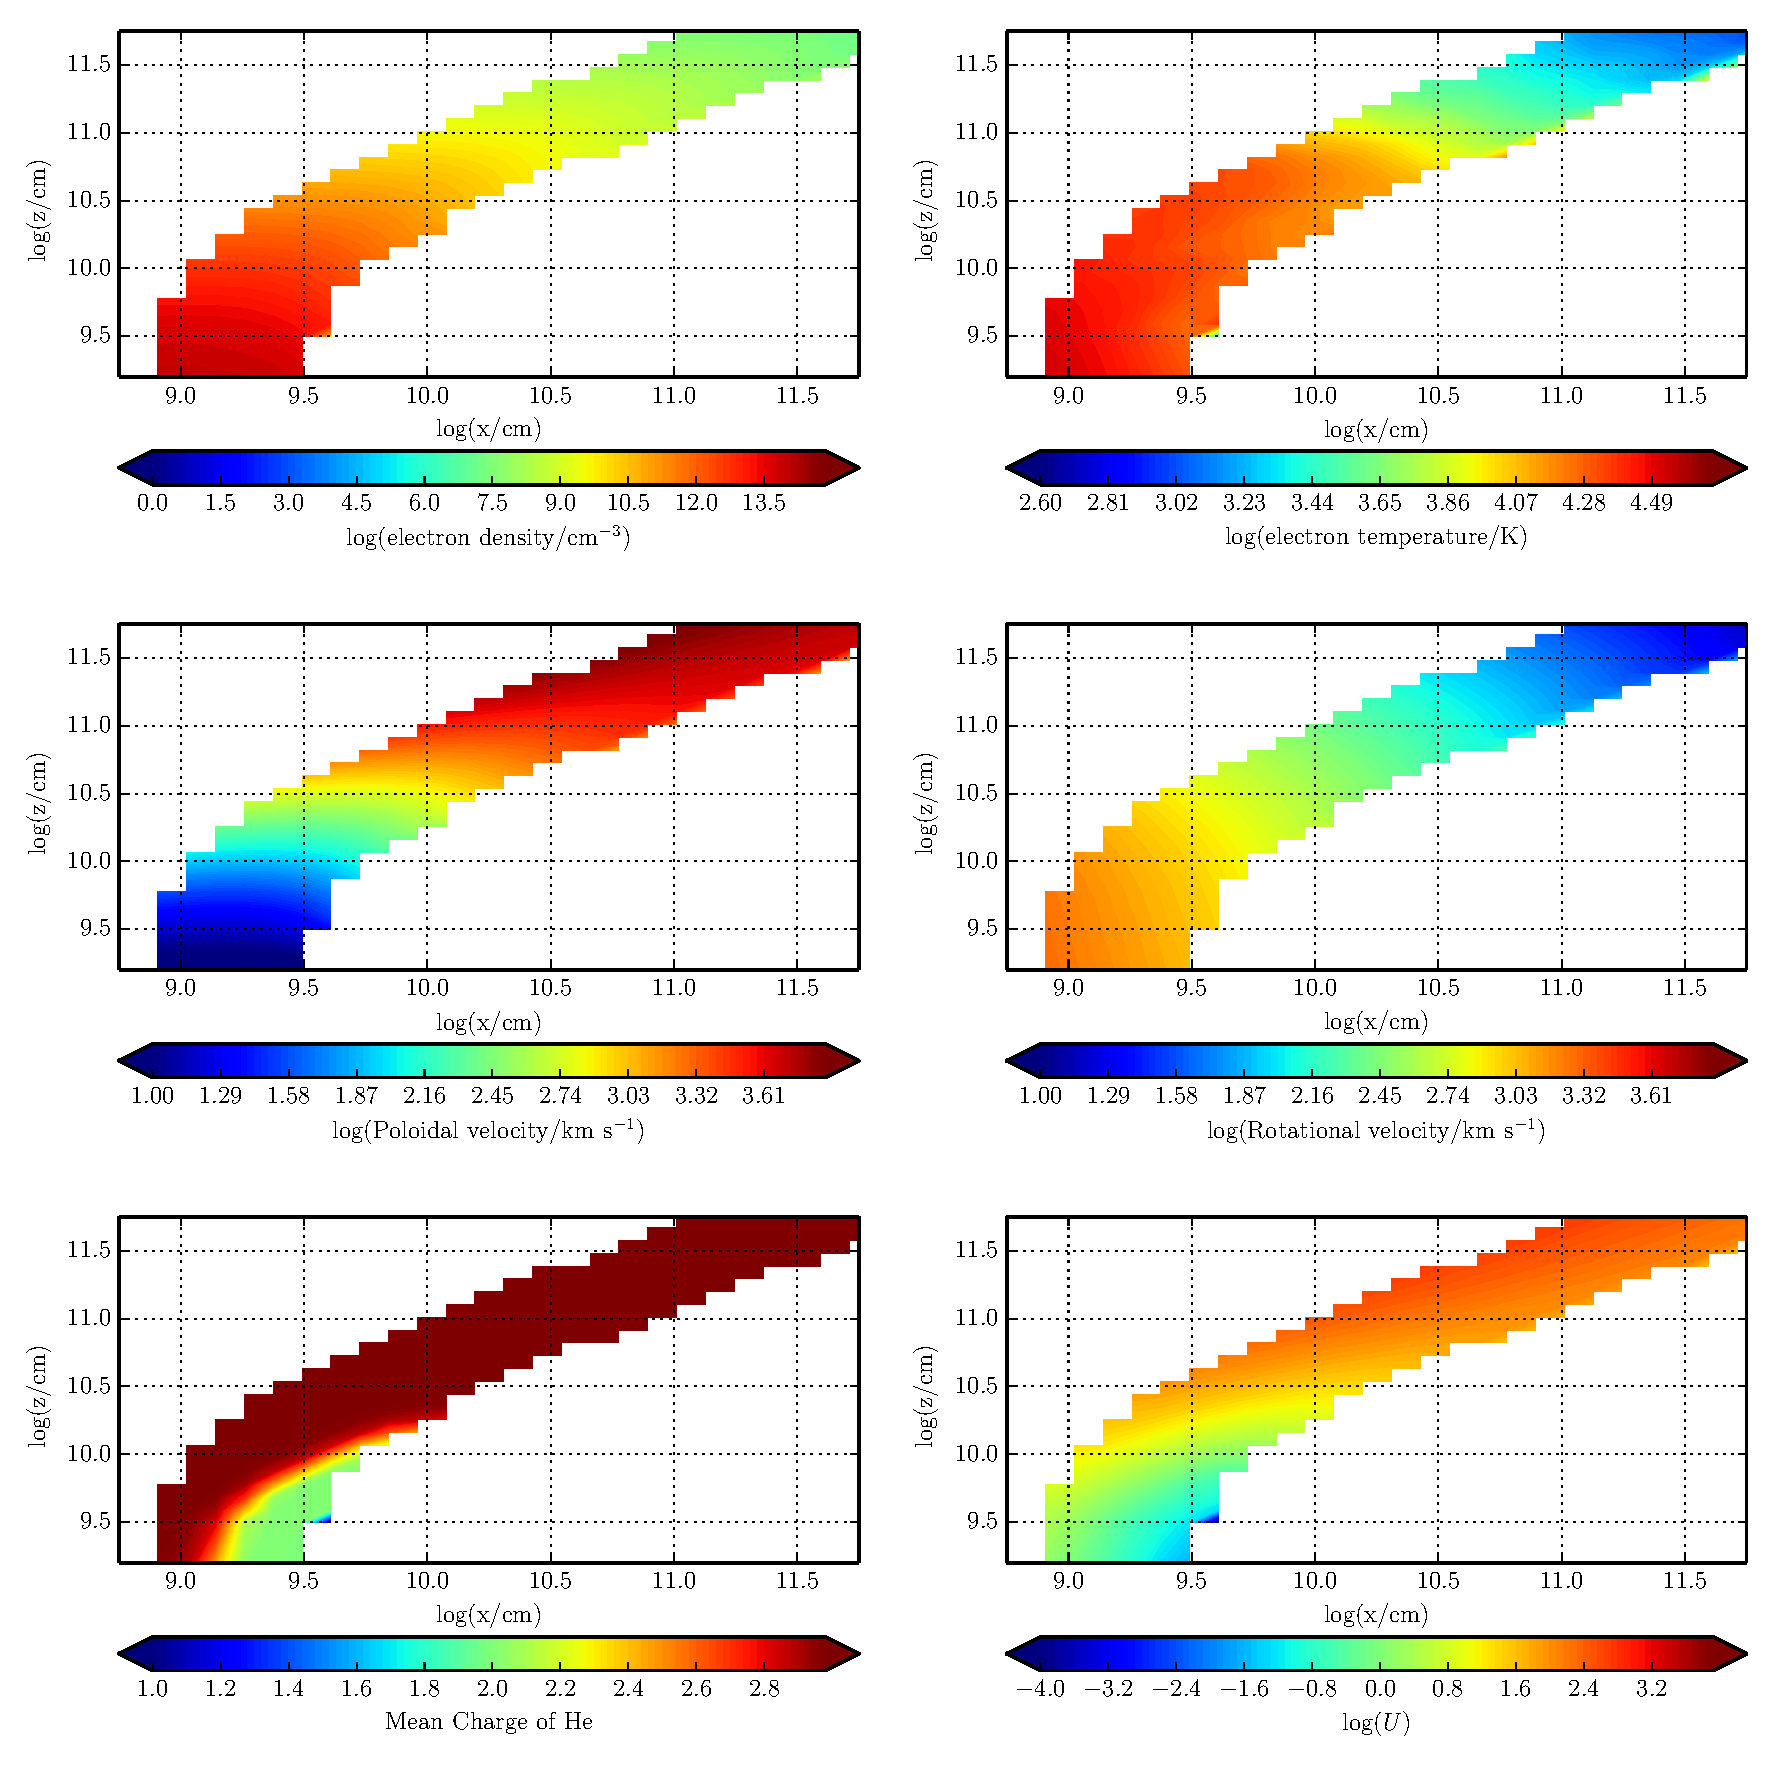
\includegraphics[width=1.0\textwidth]{figures/05-cvpaper/fig5.eps}
\caption
[The physical properties of the wind in the benchmark CV model.]
{
The physical properties of the wind -- note the logarithmic scale. 
Near the disc plane the wind is dense, with low poloidal velocities.
As the wind accelerates it becomes less dense
and more highly ionized. The dominant He ion
is almost always He III, apart from in a small
portion of the wind at the base, which is partially shielded
from the inner disc.
}
\label{wind}
\end{figure*}

\index{ionization state}\index{ionization parameter}
Fig.~\ref{wind} shows the physical and ionization structure 
of the benchmark disc wind model. The ionization parameter shown in the bottom
right panel is given by equation~\ref{eq:ip}
 The ionization parameter is a useful measure of the ionization state of a plasma, 
as it evaluates the ratio of the number density of ionizing photons to the local 
H density.

There is an obvious drop-off in density
and temperature with distance away from the disc, so any line
formation process that scales as density squared -- i.e. recombination and
collisionally excited emission -- should be expected to operate
primarily in the dense base of the outflow. Moreover, a comparison of
the rotational and poloidal velocity fields shows that rotation
dominates in the near-disc regime, while outflow dominates further out
in the wind. 

\index{photoionization}\index{simple-atom}
The ionization equation used in the `simple atom' approach used by
LK02 (see section~\ref{sec:simple_ionization}) should be a reasonable approximation to
the photoionization equilibrium in the benchmark wind model. Even
though the macro-atom treatment of H and He does affect the 
computation of the overall ionization equilibrium, the
resulting ionization state of the wind should be similar to that
found by LK02. The bottom panels in Fig.~\ref{wind} confirm that this
is the case. In particular, He is fully ionized
throughout most of the outflow, except for a small region near the
base of the wind, which is shielded from the photons produced by the
hot inner disc. In line with the results of LK02,
C\textsc{iv} is the dominant C ion throughout the wind,
resulting in a substantial absorbing column across a large range of
velocities. As we shall see, this produces the broad, deep and
blue-shifted C\textsc{iv}~$1550$~\AA\ absorption line that
is usually the most prominent wind-formed feature in the UV spectra of
low-inclination nova-like CVs.
\index{nova-like variable}

\begin{figure*}
\centering
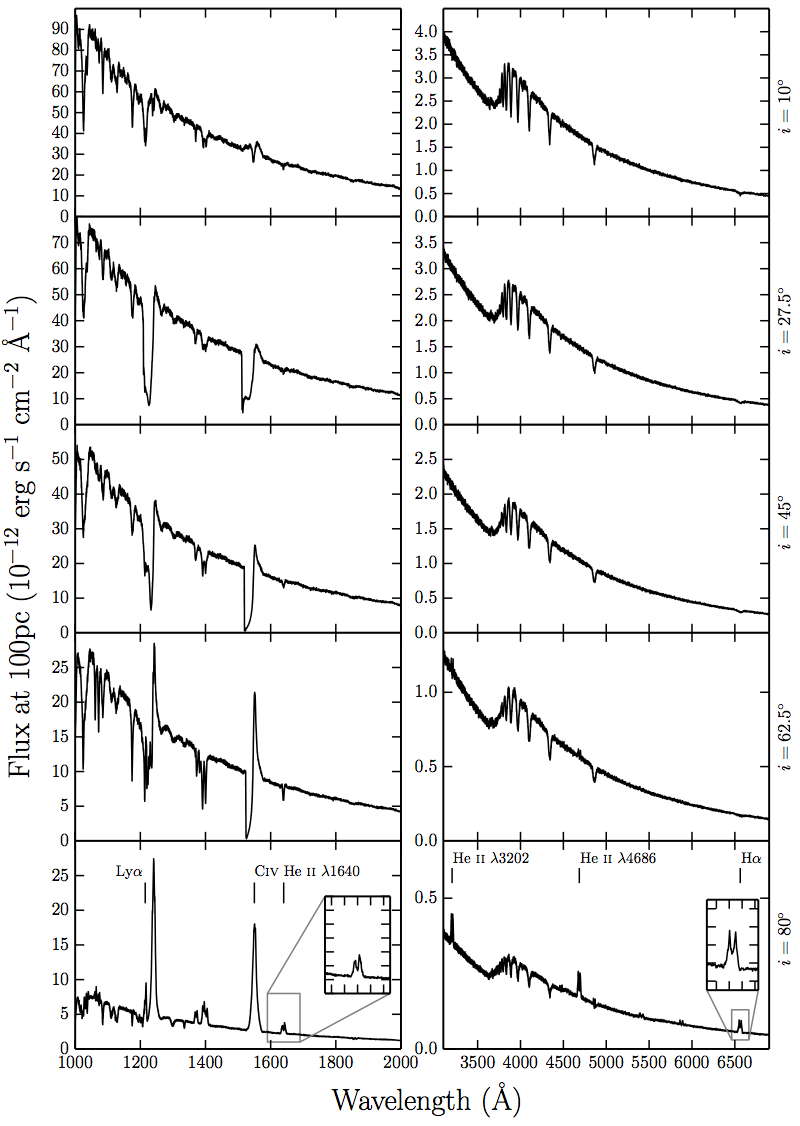
\includegraphics[width=1.0\textwidth]{figures/05-cvpaper/modela_uv_opt.png}
\caption
[UV and optical synthetic spectra from the benchmark CV model]{
UV (left) and optical (right) synthetic spectra for model A, the benchmark model,
computed at sightlines of 10, 27.5, 45, 62.5 and 80 degrees.	
The inset plots show zoomed-in line profiles for 
\heiiuv\ and \ha. Double-peaked line emission can be seen in 
\heiiuv, \heiiopt, \ha\ and some He I lines, but the 
line emission is not always sufficient to overcome the absorption
cores from the stellar atmosphere models. The model
also produces a prominent \heiioptnew\ line at high inclinations.
}
\label{spec}
\end{figure*}



\subsection{Synthetic Spectra}
\label{modela_spectrum}
\label{sec:modela_spectra}

I begin by verifying that the benchmark model still produces UV
spectra that resemble those observed in CVs. This should be
the case, since the ionization state of the wind has not changed
significantly from that computed by LK02 (see section~\ref{modela_ionization}). 
The left column of panels in Fig.~\ref{spec} shows that this expectation
is met: all of the strong metal resonance
lines -- notably N~\textsc{v}~$1240$~\AA,
Si~\textsc{iv}~$1400$~\AA\ and C~\textsc{iv}~$1550$~\AA\ -- 
are present and exhibit clear P-Cygni profiles
at intermediate inclinations. In addition, however, I now also find
that the wind produces significant Ly$\alpha$ and
He~\textsc{ii}~$1640$~\AA\ emission lines. 

Fig.~\ref{spec} (right-hand panel) and Fig.~\ref{spec_continuum}
show the corresponding optical spectra produced for
the benchmark model, and these do exhibit some emission lines
associated with H and He. There is 
a general trend from absorption lines to emission lines 
with increasing inclination, as we might expect from this wind
geometry. This trend is consistent with observations, as discussed in 
section~\ref{sec:NLs}. However, it is clear that this particular model
does not produce all of the lines seen in observations of high-state CVs.
The higher-order Balmer series lines are too weak
to overcome the intrinsic absorption from the disc atmosphere, and the wind 
fails to produce any observable emission at low and intermediate inclinations.
This contrasts with the fact that emission lines are seen 
in the optical spectra of (for example) V3885 Sgr \citep{hartley2005}
and IX Vel \citep[][see also Fig.~\ref{fig:NL_spec}]{beuermann1990}.

The emissivity of these recombination 
features scales as density squared, meaning that they form almost entirely in the 
dense base of the wind, just above the accretion disc. Here, the
velocity field of the wind is still dominated by rotation, rather than
outflow, which accounts for the double-peaked shape of the lines. In
principle, lines formed in this region can still be single peaked,
since the existence of a poloidal velocity {\em gradient} changes the
local escape probabilities (MC96). However, as
discussed further in section~\ref{sec:cv_line_shapes}, the 
radial velocity shear in the
models is not high enough for this radiative transfer effect
to dominate the line shapes.
\index{recombination continuum}\index{recombination}
\index{emission line!double-peaked}\index{emission line!single-peaked}

The Balmer jump is in absorption at all inclinations for the benchmark
model. This is due to the stellar atmospheres used to
model the disc spectrum; it is not a result of photoabsorption in the
wind. In fact, the wind spectrum exhibits the Balmer jump in {\em
emission}, but this is not strong enough to overcome the intrinsic
absorption edge in the disc spectrum. This is illustrated in
Fig.~\ref{cont}, which shows the angle-integrated spectrum of the system,
i.e. the spectrum formed by all escaping photons, separated into the
disc and wind contributions. Even though the wind-formed Balmer
recombination continuum does not completely fill in the Balmer
absorption edge in this model, it does already contribute
significantly to the total spectrum. This suggests that modest changes 
to the outflow kinematics might boost the wind continuum and produce
emergent spectra with weak or absent Balmer absorption edges. 
\index{Balmer edge}\index{stellar atmosphere}

\begin{figure}
\centering 
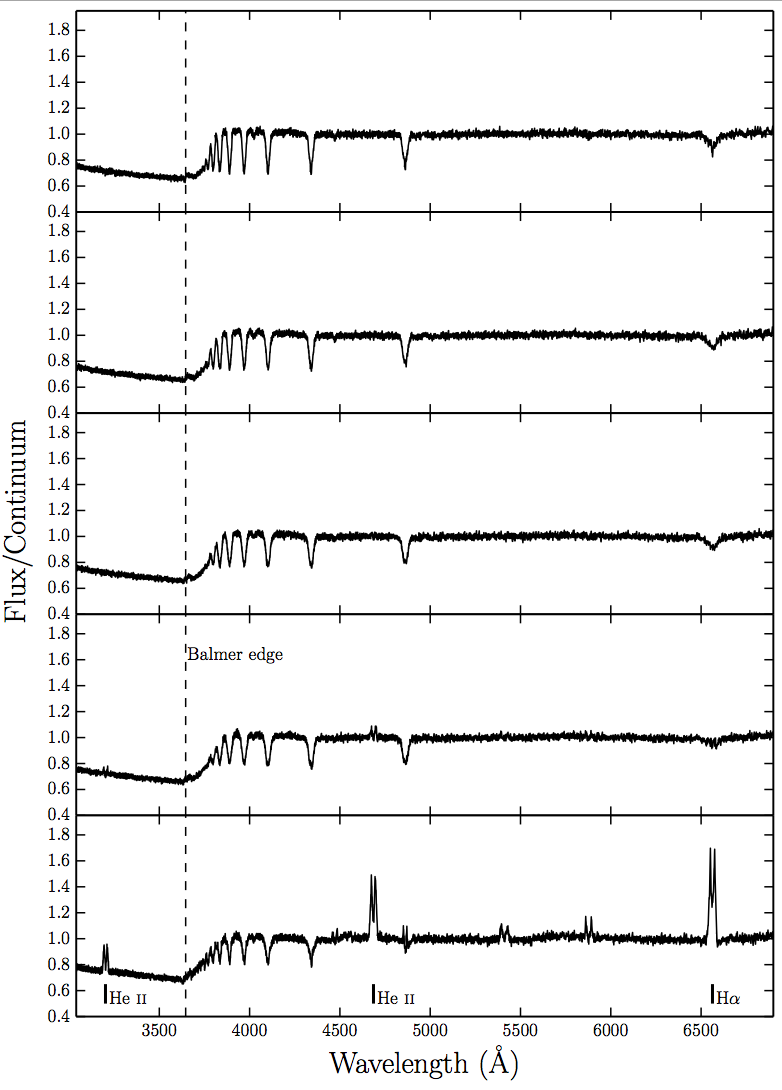
\includegraphics[width=1.0\textwidth]{figures/05-cvpaper/modela_opt_cont.png}
\caption
[Optical synthetic spectra from the benchmark CV model divided by the continuum.]
{Synthetic optical spectra from model A computed for 
sightlines of 10, 27.5, 45, 62.5 and 80 degrees. In these plots
the flux is divided by a polynomial fit to the 
underlying continuum redward of the Balmer edge, so that 
line-to-continuum ratios and the true depth of the
Balmer jump can be shown.}
\label{spec_continuum}
\end{figure} 

\begin{figure} 
\centering
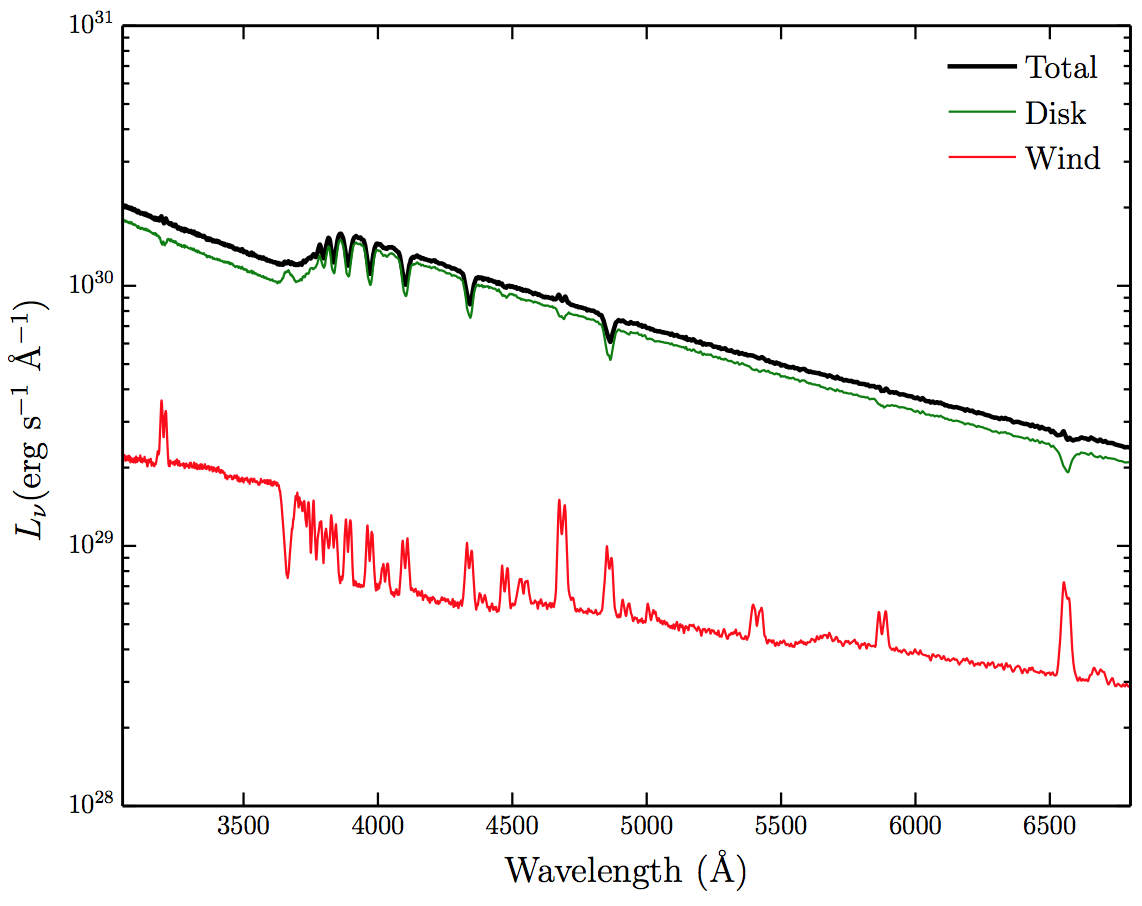
\includegraphics[width=1.0\textwidth]{figures/05-cvpaper/modela_escaping.png}
\caption
[Total packet-binned spectra across all viewing angles from the benchmark CV model.]
{Total packet-binned spectra across all viewing angles, in units
of monochromatic luminosity.
The thick black line shows the total 
integrated escaping spectrum, 
while the green line shows disc photons which escape without being reprocessed by
the wind. The red line show the contributions from reprocessed photons. 
Recombination continuum emission blueward of the Balmer 
edge is already prominent relative to other wind continuum processes, but is not sufficient
to fill in the Balmer jump in this specific model.}
\label{cont}
\end{figure} 


%\newpage



%%%%%%%%%%%%%%%%%%%%%%%%%%%%%%%%%%%%%%
%
%          REVISED MODEL
%
%%%%%%%%%%%%%%%%%%%%%%%%%%%%%%%%%%%%%%%

\section{A Revised Model Optimized for Optical Wavelengths}
\label{sec:modelb}
The benchmark model discussed in section~\ref{modela} was originally
designed to reproduce the wind-formed lines seen in the UV spectra of
high-state CVs. This model does produce some observable
optical emission, but I can now attempt to construct a model that more closely 
matches the observed optical spectra of CVs. 

Specifically, I aim to assess whether a revised model can:

\begin{itemize}
         \item account for all of the lines seen in optical spectra 
         of CVs while preserving
the UV behaviour;
         \item produce single-peaked Balmer emission lines; 
         \item generate enough of a wind-formed recombination continuum
to completely fill in the disc's Balmer absorption edge for 
reasonable outflow parameters.
\end{itemize} \index{Balmer edge}

The emission measure of a plasma is directly proportional to its density.
The simplest way to simultaneously affect the density in the wind (for fixed mass-loss rate),
as well as the velocity gradients, is by modifying the poloidal velocity
law. Therefore, I focus on just two kinematic variables:

\begin{itemize}
         \item the acceleration length, $R_v$, which controls the
        distance over which the wind accelerates to $\frac{1}{2}~v_{\infty}$;
         \item the acceleration exponent, $\alpha$, which controls the rate 
         at which the poloidal velocity changes near $R_v$.
\end{itemize} 

The general behaviour we might expect is that outflows with denser
regions near the wind base -- i.e. winds with larger $R_{v}$ and/or
larger $\alpha$ -- will produce stronger optical emission signatures. 
However, this behaviour may be moderated by the effect of the increasing
optical depth through this region, which can also affect the line profile shapes. 
In addition, modifying $R_v$ also increases the emission {\em volume}.
Based on a preliminary exploration of models with different kinematics,
I adopt the parameters listed in table~\ref{modelb_table}
for this new, `optically optimized' model (model B). 

%It is possible that other parameters, such as the launching radii and angles



\subsection{Synthetic Spectra}
\label{sec:modelb_spectra}
\begin{figure*}
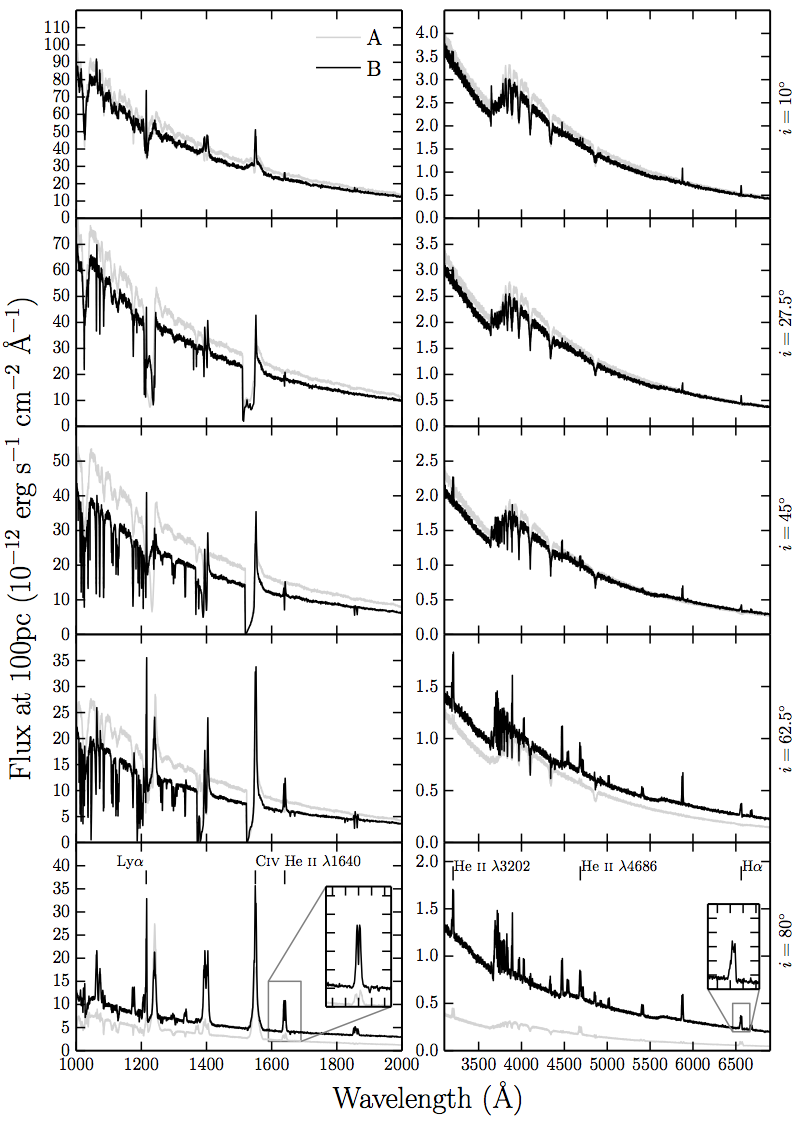
\includegraphics[width=1.0\textwidth]{figures/05-cvpaper/modelb_uv_opt.png}
\caption
[UV and optical synthetic spectra from CV model B]{
UV (left) and optical (right) synthetic spectra for model B computed at
sightlines of 10, 27.5, 45, 62.5 and 80 degrees. 
Model A is shown in grey for comparison.	
The inset plots show zoomed-in line profiles for 
\heiiuv\ and \ha. The Balmer and He
are double-peaked, albeit with narrower profiles.
Strong \heiiopt\ emission can be seen, as well as a trend
of a deeper Balmer jump with decreasing inclination.
}
\label{uvoptb}
\end{figure*}

Fig.~\ref{uvoptb} shows the UV and optical spectra for the
optically optimized model for the full range of inclinations. 
As expected, the trend from absorption to emission 
in the optical is again present, but in this revised model emission
lines in the entire Balmer series are produced at high inclinations, as well
as the observed lines 
in He~\textsc{ii} and He~\textsc{i}. This can be seen more clearly in the 
continuum-normalized spectrum in Fig.~\ref{continuumb}.

Two other features are worth noting in the optical
spectrum. First, the collisionally excited Ca~{\sc ii} emission line at $3934$~\AA\ 
becomes quite prominent in the densest models. Second, the model predicts a detectable
He~\textsc{ii} recombination line at $3202$~\AA. This is the He
equivalent of Paschen~$\beta$ and should be expected in all systems that
feature a strong He~\textsc{ii}~$4686$~\AA\ line (the He
equivalent of Paschen~$\alpha$). 
This line is somewhat unfamiliar observationally, because it 
lies bluewards of the atmospheric cut-off, but
also redwards of most ultraviolet spectra. 

\index{P-Cygni profile}
The synthetic spectra do not exhibit P-Cygni profiles in the optical lines.
This is perhaps not surprising. LK02 and SV93 originally designed such models
to reproduce the UV line profiles. Thus, most of the wind
has an ionization parameter of $\log U \sim 2$ (see Fig.~\ref{wind}).
This means H and He are mostly ionized throughout 
much of the wind and are successful in producing recombination features.
However, the line opacity throughout the wind is too
low to produce noticeable blue shifted absorption in these lines. 
It appears that the systems that exhibit such profiles must 
possess a higher degree of ionization stratification, although the lack 
of contemporary observations means it is not known for certain if the 
P-Cygni profiles in UV resonance lines and optical H and He lines exist simultaneously.
Ionization stratification could be caused by a clumpy flow, in which the 
ionization state 
changes due to small scale density fluctuations, or a stratification in density
and ionizing radiation field over larger scales.\index{clumping}
Invoking clumpiness in these outflows is not an unreasonable
hypothesis. Theories of line-driven winds predict an unstable flow
\citep{macgregor1979,owockirybicki1984,owockirybicki1985}, an
\index{line-driving}\index{line-driven instability}
simulations of CV disc winds also produce density inhomogeneities 
\citep{proga1998,pkdh2002}.
Tentative evidence for clumping being directly related to P-Cygni optical lines
comes from the fact that \cite{prinja2000}
found the dwarf nova BZ Cam's outflow to be unsteady and highly mass-loaded in outburst,
based on observations of the UV resonance lines.
This system has also exhibited P-Cygni profiles in He~\textsc{i}~$5876$~\AA
and \ha\ when in a high-state \citep{patterson1996,RN98}. 
The degree of ionization and density variation and 
subsequent line opacities may be affected by the model parameters
and the specific parameterisation adopted.

\index{resonance line}
In the UV, the model still produces all the observed lines, 
and deep P-Cygni profiles are produced in the normal resonance lines,
as discussed in section~\ref{sec:modela_spectra}. However, the UV spectra also
display what is perhaps the biggest problem with this revised model,
namely the strength of resonance line emission 
at low and intermediate inclinations.
In order to generate strong optical wind signatures, I have adopted wind
parameters that lead to very high densities at the base of the wind
($n_e\sim10^{13}-10^{14}$~cm$^{-3}$). This produces
the desired optical recombination emission, but also increases the
role of collisional excitation in the formation of the UV resonance
lines. This explains the pronounced increase in the emission component 
of the C\textsc{iv} $1550$~\AA\ resonance line, for example, relative to
what was seen in the benchmark model (compare Figures~\ref{spec} and
\ref{uvoptb}). The strength of this component in the revised model 
is probably somewhat too high to be consistent with UV observations 
of high-state CVs \citep[see e.g.][]{long1991,long1994, noebauer}.
\index{recombination}
\index{collisional excitation}

\subsection{Continuum Shape and the Balmer Jump}
\index{Balmer edge}\index{recombination continuum}
The wind now also has a clear effect on the continuum shape,
as shown by Fig.~\ref{modelb_escape}. In fact, the majority of the
escaping spectrum has been reprocessed in some way by the wind,
either by electron scattering (the wind is now moderately Thomson-thick),
or by bound-free processes. This is demonstrated by the flatter spectral shape
and the slight He photoabsorption edge present in the optical spectrum 
(marked in Fig.~\ref{continuumb}). This reprocessing is also
responsible for the change in continuum level between models A and B.
In addition, Figures~\ref{uvoptb}, \ref{continuumb} 
and \ref{modelb_escape} clearly demonstrate that the wind produces
a recombination continuum sufficient to completely fill in the Balmer jump
at high inclinations.\footnote{Note that the apparent absorption feature 
just redward of the Balmer jump in these models is artificial. It is
caused by residual line blanketing in the stellar atmospheres, which
the models cannot fill in since they employ a 20-level H atom.}
This might suggest that Balmer continuum emission from a wind can be important 
in shaping the Balmer jump region, as
suggested by \cite{KLWB98} and \cite{hassall}.

It should be acknowledged, however,\index{Balmer edge}
that the Balmer jump in high-state CVs would naturally weaken at
high inclinations due to limb darkening effects \citep{ladous1989, ladous1989b}. 
Although simple limb darkening law which affects \index{limb darkening}
the emergent flux at each inclination is included,
it is not a {\em frequency dependent} opacity in the model.
As a result, the efficiency of filling in the Balmer jump
should really be judged at low and medium inclinations, 
where, although prominent, the recombination continuum does
not overcome the disc atmosphere absorption. 
In addition, this effect 
could mean that any model which successfully fills in the 
jump at low inclinations could lead to a Balmer jump 
in emission at high inclinations.
Furthermore, in this particular model,
approximately $10\%$ of the overall luminosity ultimately
hits the surface of one of the photon sources and is destroyed.
Neglecting this backscattered radiation could have a small effect on the temperature
and ionization structure of the disc and the wind base. Irradiation of the disc
by the WD is insignificant, as the high accretion rate causes the disc 
to dominate the emergent luminosity (see e.g. Fig.~\ref{cv_model_sed}).
In any case, to properly understand the 
effect of inclination and irradiation on the resultant 
Balmer jump, a fully self-consistent
radiative transfer calculation of both the disc atmosphere
and connected wind is required. 
\index{recombination continuum}\index{limb darkening}\index{stellar atmosphere}

\begin{figure} 
\centering
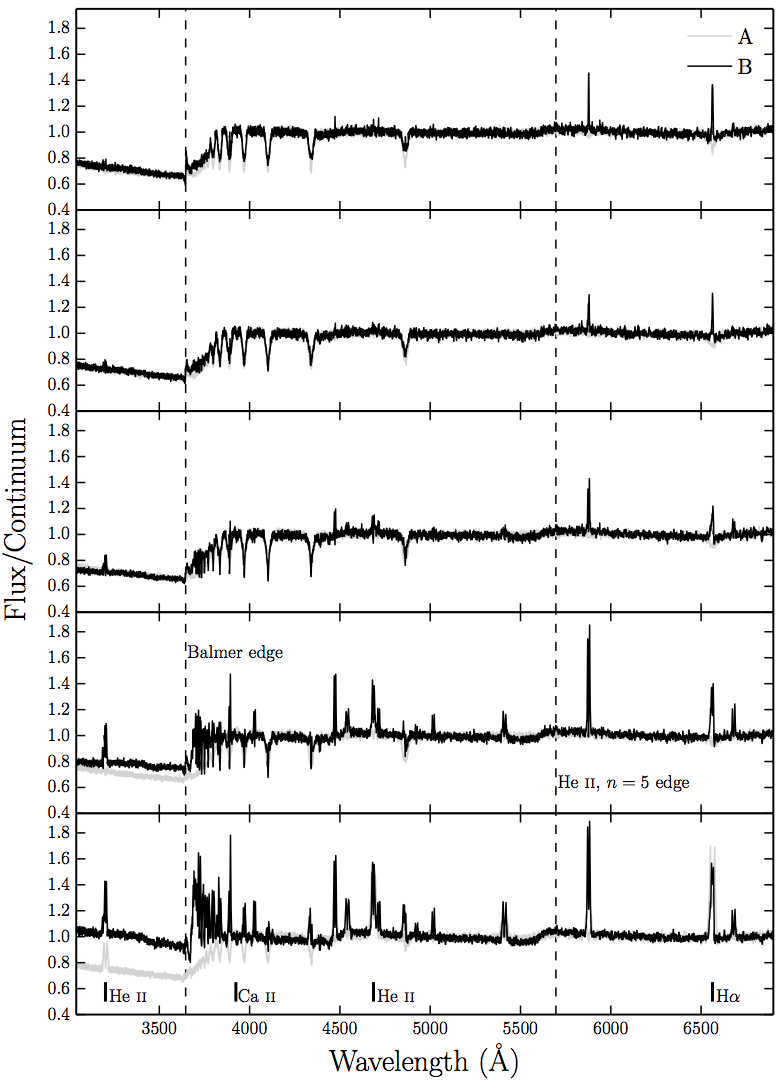
\includegraphics[width=1.0\textwidth]{figures/05-cvpaper/modelb_opt_cont.png}
\caption
[Optical synthetic spectra from CV model B divided by the continuum.]{
Synthetic optical spectra from model B computed for 
sightlines of 10, 27.5, 45, 62.5 and 80 degrees. 
Model A is shown in grey for comparison.
In these plots the flux is divided by a polynomial fit to the 
underlying continuum redward of the Balmer edge, so that 
line-to-continuum ratios and the true depth of the
Balmer jump can be shown.
}
\label{continuumb}
\end{figure} 

\begin{figure} 
\centering
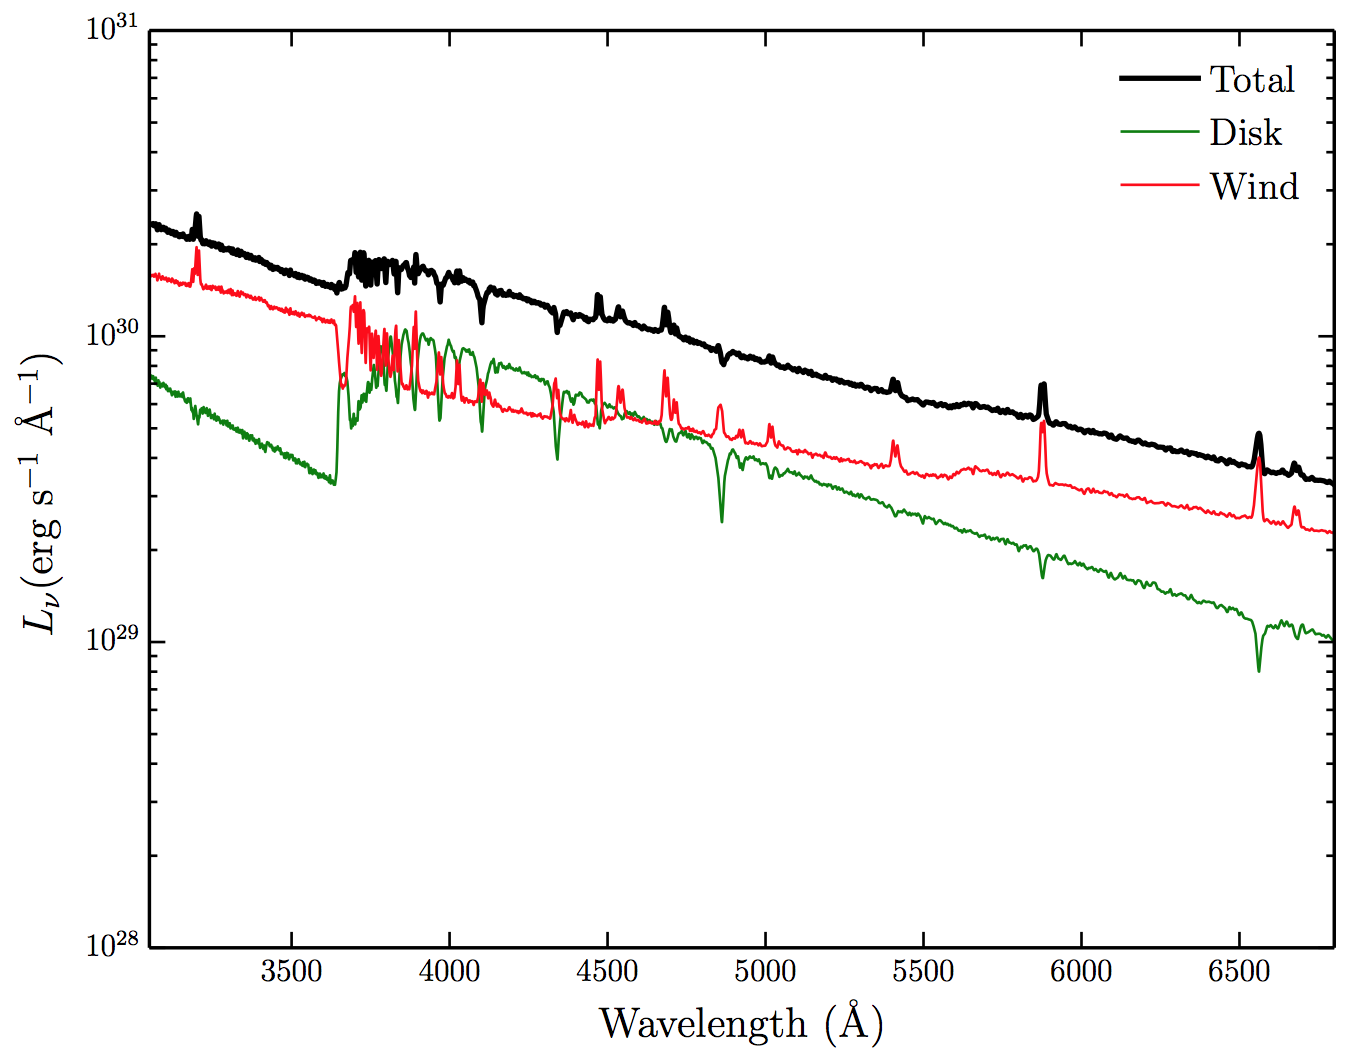
\includegraphics[width=1.0\textwidth]{figures/05-cvpaper/modelb_escaping.png}
\caption
[Total packet-binned spectra across all viewing angles from CV model B.]
{Total packet-binned spectra across all viewing angles, in units
of monochromatic luminosity. 
The thick black line shows the total 
integrated escaping spectrum, 
while the green line shows disc photons which escape without being reprocessed by
the wind. The red line show the contributions from reprocessed 
photons. 
In this denser model the reprocessed contribution is significant compared
to the escaping disc spectrum. The Balmer continuum emission is prominent, and
the wind has a clear effect on the overall spectral shape.}
\label{modelb_escape}
\end{figure} 

\begin{figure}
\centering
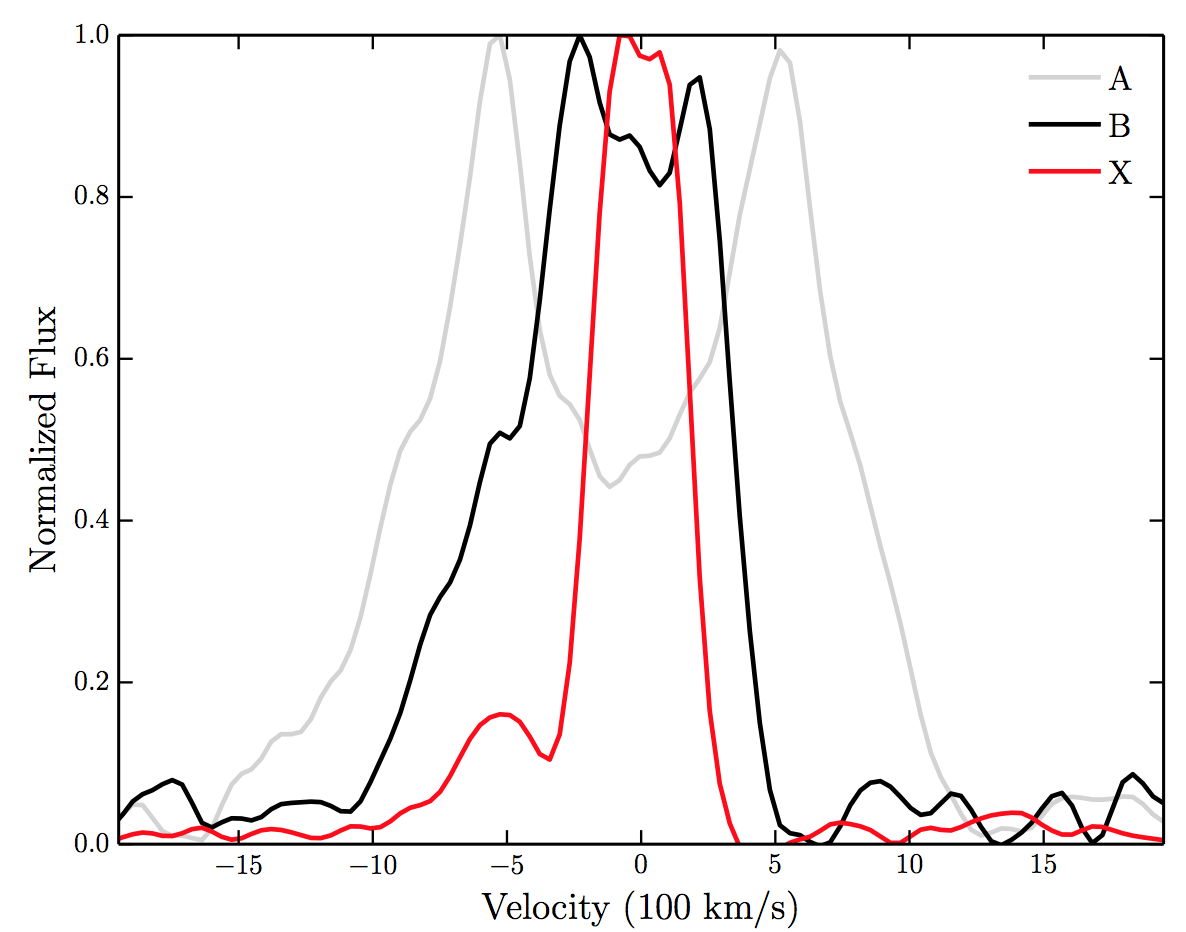
\includegraphics[width=1.0\textwidth]{figures/05-cvpaper/mc.png}
\caption
[\ha\ line profiles from CV models A, B and X]
{
\ha\ line profiles, normalized to 1, plotted in velocity space 
for three models with varying kinematic 
properties, computed at an inclination of $80^\circ$.
The benchmark model and the improved optical
model described in section~\ref{sec:modelb} are labeled as A and B respectively,
and a third model (X) which has an increased acceleration length of 
$R_v = 283.8~R_{WD}$, and $\alpha=4$ is also shown. 
The $x$-axis limits correspond to the Keplerian velocity at 
$4~R_{WD}$, the inner edge of the wind.
There is a narrowing of the lines, and a single-peaked line in model X.
This is not due to radial velocity shear (see section~\ref{sec:cv_line_shapes}).
}
\label{halpha}
\end{figure} %fullpage






\subsection{Line Profile Shapes: Producing Single-Peaked Emission}
\label{sec:cv_line_shapes}
\index{emission line}\index{emission line!double-peaked}\index{emission line!single-peaked}
Fig.~\ref{halpha} shows how the H$\alpha$ profile changes with the kinematics of the wind for 
an inclination of $80^\circ$. The main prediction is that dense, slowly accelerating 
wind models produce narrower emission lines. This is {\em not} due to radial 
velocity shear. As stated by MC96, that mechanism can only work if poloidal 
and rotational velocity gradients satisfy $(dv_l/dr)/(dv_\phi/dr) \gtrsim 1$; in 
these models, this ratio is always $\lesssim 0.1$. Instead, the narrow lines predicted 
by the denser wind models can be traced to the base of the outflow becoming optically 
thick in the continuum, such that the line emission from the base of the wind
cannot escape to the observer. In such models, the `line photosphere'
(the $\tau \simeq 1$ surface of the line-forming region) moves outwards, towards larger 
vertical and cylindrical distances. This reduces the predicted line widths, since the 
rotational velocities -- which normally provide the main line broadening mechanism at 
high inclination -- drop off as $1/r$ in the outflow. This $1/r$ behaviour occurs due to the wind
conserving specific angular momentum from its initial Keplerian rotation 
(see equation~\ref{eq:vrot}). The fact that the MC96 
mechanism does not significantly affect the line profiles in this specific model 
does not mean that it could not be at work in CV winds. For example, it would be worth investigating
alternative prescriptions for the wind velocity field, as well as the possibility that the 
outflows may be clumped. An inhomogeneous flow 
(which has been predicted in CVs; see section~\ref{sec:modelb_spectra})
might allow large radial velocity shears to exist while still 
maintaining the high densities needed to produce the required level of emission.
However, such an investigation is beyond the scope of the present study.

In these models, single-peaked line profiles are produced once the line forming region 
has been
pushed up to $\sim 10^{11}$~cm ($\sim150~R_{WD}$) above the disc plane. 
This number may seem unrealistically large, but the vertical extent of 
the emission region is actually not well constrained observationally. 
In fact, multiple observations of eclipsing NLs show that the H$\alpha$ 
line is only moderately eclipsed compared to the continuum 
\citep[e.g.][see also section~\ref{sec:rwtri}]{baptista2000,groot2004}, 
implying a significant vertical extent for the line-forming 
region. This type of model should therefore not be ruled out {\em a priori}, 
but this specific model was not adopted as the optically optimized model
due to its unrealistically high continuum level in eclipse. 

\index{emission line!double-peaked}\index{emission line!single-peaked}
Observations could help to assess the viability of this scenario, in which lines 
are single peaked due to being formed high above the disc plane. The line formation
region is roughly cospatial with the main recombination continuum emission region.
Thus, the in and out of eclipse continuum levels of high-inclination CVs should be 
compared to see how much of any extended wind emission is occulted by the 
donor star, allowing limits to be placed on
the emission region size. Directly imaging the continuum emission region may prove harder.
At a typical NL distance of $200$~pc \citep[e.g.][]{knigge2006,mizusawa2010}, 
the angular size of a region of size $10^{11}$~cm is approximately $5$~mas. This lies beyond the 
capabilities of the 
{\sl Hubble Space Telescope}\footnote{http://www.spacetelescope.org/about/general/instruments/wfc3/} 
and the future 
{\sl James Webb Space Telescope}\footnote{http://jwst.nasa.gov/facts.html}.
If the emission region is more extended, on the order of $10^{12}$~cm, resolving it may just 
be possible in the case of the closest NLs and high-state 
DNe \citep[at $\sim100$~pc, e.g.][]{millerjones2013}, which would represent 
the first direct observation of a disc wind. Generally, however, this specific
observation appears to be challenging for even the next generation of 
space telescopes.
\index{James Webb Space Telescope}\index{nova-like variable}
\index{disc wind}\index{Hubble Space Telescope}\index{dwarf nova}
\index{recombination continuum}


\subsection{Sensitivity to Model Parameters}
\label{sec:cv_params}
This revised model demonstrates that one can achieve a more
realistic optical spectrum by altering just two kinematic parameters. 
However, it may also be possible to achieve this by modifying
other free parameters such as $\dot{M}_{W}$, the opening angles of the wind and the 
inner and outer launch radii. For example, increasing the mass-loss rate of the wind
increases the amount of recombination emission (which scales with density squared), 
as well as lowering the ionization parameter and increasing the optical depth through the wind. 
Larger launching regions and covering factors tend to lead to a larger emitting volume, 
but this is moderated by a decrease in density 
for a fixed mass-loss rate. I also note that the inner radius of $4~R_{WD}$ adopted by SV93 
affects the emergent UV spectrum seen at inclinations $<\theta_{\mathrm{min}}$ as 
the inner disc is uncovered. This causes less absorption in the UV resonance lines,
but the effect on the optical spectrum is negligible.
I have verified this general behaviour, but
I suggest that future work should investigate the effect of these parameters in more detail,
as well as incorporating a treatment of clumping.
If a wind really does produce the line and continuum emission seen in optical spectra of high-state CVs, then
understanding the true mass-loss rate and geometry of the outflow is clearly important.


\subsection{Comparison to RW Tri}
\label{sec:rwtri}
\begin{figure*}
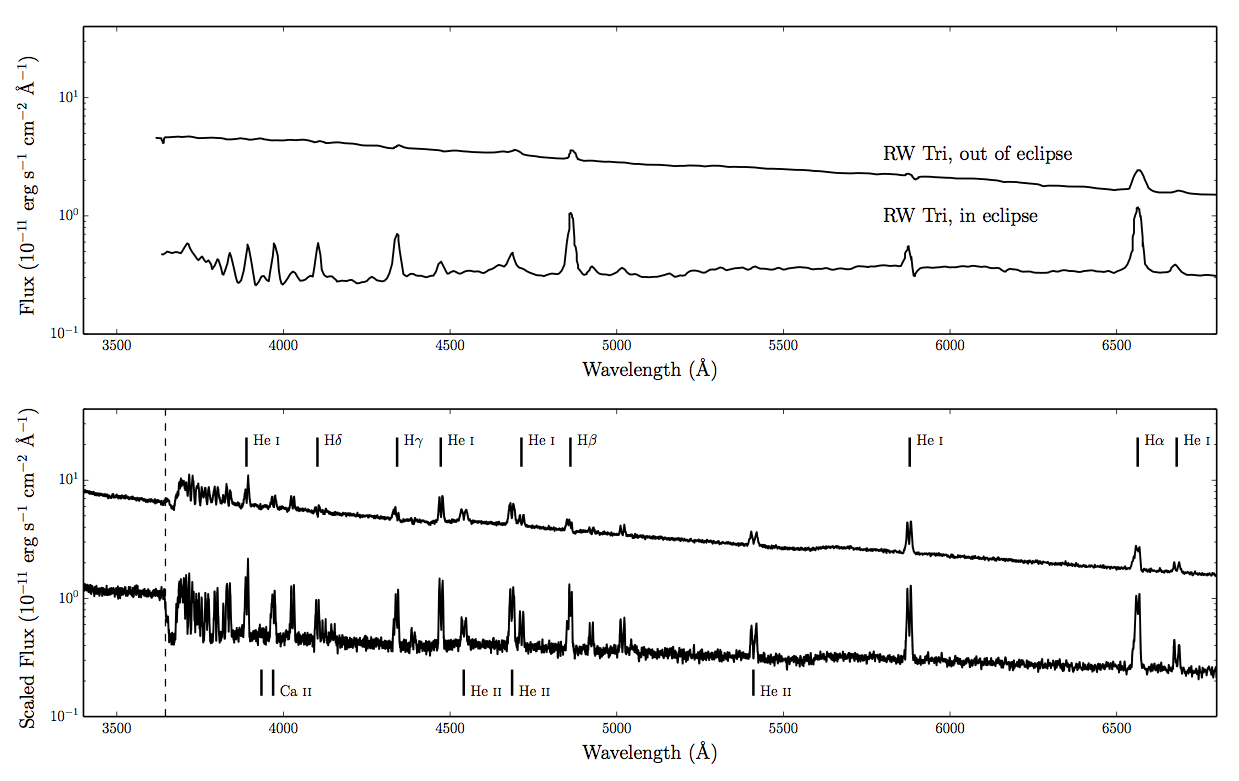
\includegraphics[width=0.9\textheight, angle=270]{figures/05-cvpaper/fig13.png}
\caption
[In and out of eclipse spectra from model B compared to the high
inclination NL RW Tri]
{{\sl Top Panel:} In and out of eclipse spectra of the high
inclination NL RW Tri. {\sl Bottom Panel:} In and out of eclipse synthetic
spectra from model B.
The artificial `absorption' feature just redward of the Balmer jump
is due to the reasons described in section 5.2.}
\label{rwtricomp}
\end{figure*}
\index{RW Tri}
Fig.~\ref{rwtricomp} shows a comparison of the predicted
out-of-eclipse and mid-eclipse spectra against observations of the
high-inclination nova-like RW~Tri. The inclination of RW Tri is
somewhat uncertain, with estimates including $70.5^\circ$
\citep{smak1995}, $75^\circ$ \citep{groot2004}, $80^\circ$
\citep{longmore1981} and $82^\circ$\citep{frankking1981}. Here, we
adopt $i = 80^\circ$, but the qualitative conclusions are not
particularly sensitive to this choice. 
I follow LK02 in setting the value of $r_{\mathrm{disc}}(\mathrm{max})$ (the maximum radius of the accretion disc)
to $34.3~R_{WD}$. When compared to the semi-major axis of RW Tri,
this value is perhaps lower than one might 
typically expect for NLs \citep{harropallinwarner1996}. 
However, it is consistent
with values inferred by \cite{rutten1992}.
I emphasize that this model is in no sense a fit to this -- or any other -- data set.


The similarity between the synthetic and observed spectra is
striking. In particular, the revised model produces strong emission in
all the Balmer lines, with line-to-continuum ratios comparable to
those seen in RW Tri. Moreover, the line-to-continuum contrast
increases during eclipse, as expected for emission produced in a disc
wind. This trend is in line with the observations of RW~Tri, and it
has also been seen in other NLs, including members of the SW~Sex class
\citep{neustroev2011}. As noted in section~\ref{sec:modelb_spectra}, the majority
of the escaping radiation has been reprocessed by the wind in some way
(particularly the eclipsed light).

However, there are also interesting differences between the revised
model and the RW Tri data set. For example, the synthetic spectra exhibit
considerably stronger He~{\sc ii} features than the observations,
which suggests that the overall ionization state of the model is
somewhat too high. As discussed in section~\ref{sec:cv_line_shapes}, 
the optical lines are narrow, but double-peaked. 
This is in contrast to what is generally seen in observations
of NLs, although the relatively low resolution of the RW Tri
spectrum makes a specific comparison difficult. In order to demonstrate
the double-peaked nature of the narrower lines, I do not 
smooth the synthesized data to the resolution of the RW Tri dataset.
If the data was smoothed, the \ha\ line would appear single-peaked.
\index{RW Tri}\index{emission line!double-peaked}\index{emission line!single-peaked}

\subsection{A Note on Collision Strengths}
\label{sec:coll_bl}

\index{bound-bound collision strength}
\index{van Regemorter approximation}
\index{gaunt factor!effective (collisional)}
\py\ uses the \cite{vanregemorter} approximation 
(see section~\ref{sec:coll}) to calculate collision rates.
This approach uses an effective gaunt factor, $\bar{g}$, of
order unity. To conduct these specific simulations a value of $\bar{g}=1$ 
was adopted. There are two main concerns when using this approach.
The first is related to accuracy, as poorly estimating collision strengths
could lead to incorrect heating and cooling balance in the flow, with
knock-on effects on the emergent spectrum. This is of particular concern
here as line heating is the dominant heating mechanism in the dense 
base of the wind. I have verified that the main conclusions of this study
are fairly insensitive to the gaunt factor; for example, if I adopt
$\bar{g}=0.2$ as suggested by, e.g., \cite{ferland2005} than the wind still
produces a host of recombination lines. 
If improved collision strengths were to significantly reduce the wind temperature
a boundary layer might
actually be required to produce the higher ionization lines such as 
\heiiopt\ \citep[see e.g.][]{hoare1991}, arguably making the model
more realistic.

The second concern is that 
collisions between radiatively forbidden transitions are not taken into 
account when one splits levels into $l$- and $s$-subshells, as well
as principal quantum number, $n$ (as I have done with He~\textsc{i}; 
see section~\ref{sec:atomic_data}). However, I have verified that
in this case the plasma is dense enough, and ionized enough, 
that recombination dominates the level populations, at least in 
the regions responsible for the optical line emission. In other words, two levels
that are linked only by a forbidden transition have their relative populations
determined by their recombination rates from the upper ion.
Nevertheless, for future efforts, it would be desirable to include
collisional data for forbidden transitions, an effort that has now
been started (see chapter 7).
\index{bound-bound collision strength}
\index{gaunt factor!effective (collisional)}
\index{forbidden line}
\index{atomic data}





%%%%%%%%%%%%%%%%%%%%%%%%%%%%%%%%%%%%%%
%
%          CONCLUSIONS
%
%%%%%%%%%%%%%%%%%%%%%%%%%%%%%%%%%%%%%%%


\section{Conclusions}
\label{sec:cv_conclusions}

\index{disc wind}\index{recombination continuum}
I have investigated whether a disc wind model designed to reproduce
the UV spectra of high-state CVs would also have a significant effect
on the optical spectra of these systems. I find that this is indeed
the case. In particular, the model wind produces H and He
recombination lines, as well as a recombination continuum blueward of
the Balmer edge. The spectra do not show P-Cygni profiles
in the optical H and He lines, which are seen in a small fraction of CV 
optical spectra. Possible reasons for this are briefly discussed in 
section~\ref{sec:modelb_spectra}.

A revised benchmark model was also constructed
to more closely match the optical spectra of high-state CVs. This
optically optimized model produces all the prominent optical lines in
and out of eclipse and achieves reasonable verisimilitude with the
observed optical spectra of RW Tri. However, this model also has
significant shortcomings. In particular, it predicts
stronger-than-observed He~{\sc ii} lines in the optical region and too
much of a collisionally excited contribution to the UV resonance lines. 
Incorporating more accurate collisional data into \py\ will help
assess this discrepancy in more detail.

Based on these results, I argue that recombination emission 
from outflows with sufficiently high densities and/or optical depths 
might produce the optical lines observed in CVs. It may also 
fill in the Balmer absorption edge in the spectrum of the accretion disc, 
thus accounting for the absence of a strong edge in observed CV spectra.
In section~\ref{sec:cv_line_shapes}, I demonstrated that
although the double peaked lines narrow and 
single-peaked emission can be formed in the densest models, 
this is not due to the radial velocity shear mechanism proposed by MC96.
I suggest that `clumpy' line-driven winds or a different
wind parameterization may nevertheless allow this mechanism to work.
I also note the possibility that, as seen in the densest models I have presented, 
the single-peaked lines are formed well above the disc, where 
rotational velocities are lower.

It is not yet clear whether a wind model such as this can
explain all of the observed optical features of high-state CVs --
further effort is required on both the observational
and modelling fronts. However, this work demonstrates that disc winds may
not just be responsible for creating the blue-shifted absorption and
P-Cygni profiles seen in the UV resonance lines of high-state CVs, but
can also have a strong effect on the optical appearance of these
systems. In fact, most of the optical features characteristic of CVs
are likely to be affected -- and possibly even dominated -- by their disc
winds. Given that optical spectroscopy plays a central role in
observational studies of CVs, it is critical to know 
where and how these spectra are actually formed. I believe it is high
time for a renewed effort to understand the formation of spectra in
accretion discs and associated outflows. 


 % Experiment 1

% \chapter{Testing Quasar Unification: Radiative Transfer In Clumpy Winds}

%%\epigraph{``Don't do it, James. CVs will ruin your life.''}{{\sl Retha Pretorius}}

{\em This chapter is based on the publication:

Matthews J. H., Knigge C., Long K. S., Sim S. A., Higginbottom N., Mangham S. W., 
`Testing quasar unification: radiative transfer in clumpy winds',
2016, MNRAS, 458, 293.}


%%%%%%%%%%%%%%%%%%%%%%%%%%%%%%%%%%%%%%
%
%          INTRODUCTION
%
%%%%%%%%%%%%%%%%%%%%%%%%%%%%%%%%%%%%%%%
%% Codes
\def\py{\textsc{Python}}
\def\tar{\textsc{Tardis}}
\def\cld{\textsc{Cloudy}}
\def\agn{\textsc{Agnspec}}


%% Lines and ions
\def\civ{C~\textsc{iv}}
\def\nv{N~\textsc{v}}
\def\hei{He~\textsc{i}}
\def\heii{He~\textsc{ii}}
\def\heiiline{He~\textsc{ii}~$4686$\AA}
\def\mg{Mg~\textsc{ii}}
\def\al{Al~\textsc{iii}}
\def\heii{He~\textsc{ii}}
\def\ovi{O~\textsc{vi}}
\def\la{Ly~$\alpha$}
\def\ha{H$\alpha$}
\def\hb{H$\beta$}
\def\civline{C~\textsc{iv}~$1550$\AA}
\def\nvline{N~\textsc{v}~$1240$\AA}
\def\mgline{Mg~\textsc{ii}~$2800$\AA}


%% Journal definitions
\def\araa{ARAA}
\def\nat{Nature}
\def\apjl{ApJ Letters}
\def\aapr{AAPR}
\def\ssr{SSR}
\def\apj{ApJ}
\def\apjs{ApJs}
\def\pasp{PASP}
\def\aap{A\&A}
\def\mnras{MNRAS}
\def\aj{AJ}
\def\rmxaa{RMXAA}
\def\aaps{A\&As}
\def\LA{Lyman\thinspace$\alpha$}

\newcommand{\EXPN}[2]{\mbox{$#1\times 10^{#2}$}}
\newcommand{\EXPU}[3]{\mbox{\rm $#1 \times 10^{#2} \rm\:#3$}}  % exponent with units
\newcommand{\POW}[2]{\mbox{$\rm10^{#1}\rm\:#2$}}
\def\LUM{\:{\rm erg\:s^{-1}}}
\def\FLUX{\:{\rm erg\:cm^{-2}\:s^{-1}}}
\def\OIGS{\:{\rm erg\:cm^{-2}\:s^{-1}\:\AA^{-1}}}

\section{Introduction}

In the earlier chapters I presented the evidence for accretion disc
winds in quasars and luminous AGN, and showed how they may be responsible
for more than just the broad absorption lines and P-Cygni profiles
seen in quasar spectra. In particular, they offer a natural way to
{\em unify} much of the complex phenomenology into one simple picture.

Here, I aim to test that picture using \py, with
the specific aim of determining whether it is possible to 
simulate the properties of the spectra of AGN, including BALQSOs, 
using simple kinematic prescriptions for biconical disc winds. 
Past results have been encouraging; H13
produced simulated spectra that resembled that of BALQSOs, as long as 
the luminosity of the X-ray source was relatively low, of order 
\POW{43}{\LUM} and the mass loss rate was relatively high, of order the 
mass accretion rate.  However, at higher X-ray luminosities, the wind was
so ionized that UV absorption lines were not produced.  In addition, and 
in part due to limitations in our radiative transfer code, the model failed 
to produce spectra with strong emission lines at any inclination angle.

Here I attempt to address both of these issues, by
introducing clumping into \py\ and a more complete
treatment of H and He into the radiative transfer calculations.
Thus, the simulations presented in this chapter treat H \& He as full
macro-atoms, and model metals as simple-atoms as described extensively
in chapter 3. In order to correctly model the ionizing spectrum for simple-atoms 
I dispense with the ML93 modified Saha approach and fully solve the ionization
balance using the spectral modelling approach described 
in section~\ref{sec:simple_ionization}. Macro-atoms still have their
ionization and excitation states calculated from MC estimators.

The kinematic model used once again follows the SV93
prescription, and is described, together with the clumping 
implementation, in section~\ref{sec:clumpy_wind_model}.
Section~\ref{sec:qso_results} contains the results from a clumped model, 
with comparisons to observational data, as well as some discussion. 
Further discussion and examination of sensitivity to model parameters
and viewing angle can be found in section~\ref{sec:qso_discuss}, which
expands somewhat on the work presented in \citep{M16}.
Finally, I summarise the findings in section~\ref{sec:qso_conclusions}.

% The spectra of 
% quasars and luminous active galactic nuclei (AGN) 
% typically exhibit a series of strong emission lines
% with an underlying blue continuum - the so-called {\sl `big blue bump'} (BBB). 
% The BBB is often attributed to emission from a 
% geometrically thin, optically thick accretion disc surrounding the central black hole (BH), similar to that described by \cite{shakurasunyaev1973}.
% In addition to the {\em inflowing} accreting material, 
% {\em outflows} are ubiquitous in AGN
% and quasars \citep{kellerman1989,ganguly2008}. These outflows can take the form of 
% highly collimated radio jets \citep[e.g.][]{hazard1963,potash1980,perley1984,marscher2006}, 
% or mass-loaded `winds' emanating from the accretion disc 
% \citep{weymann1991,turnermiller2009}. 
% Outflows in AGN offer a 
% potential feedback mechanism through which the central source can 
% affect its environment \citep{king2003,king2005,fabian2012}
% -- feedback that is required in models of galaxy evolution \citep{springel2005}
% and may explain the `$M-\sigma$' relation \citep{silkrees1998,haring2004}.

% Perhaps the clearest evidence of outflows in AGN is  
% the blueshifted ($\sim 0.1c$) broad absorption lines (BALs) in the 
% ultraviolet seen in approximately $20\%$ of quasars
% \citep{weymann1991, knigge2008, allen2011}.
% The simplest explanation for the incidence of 
% BAL quasars (BALQSOs) is in terms of an accretion disc wind. 
% According to this paradigm, a biconical wind rises from 
% the accretion disc and the BALQSO fraction is associated with
% the covering factor of the outflow. 
% Polarisation studies suggest that the wind is roughly equatorial
% \citep{goodrich1995, cohen1995}, although there is also evidence
% for polar BAL outflows  in radio-loud (RL) sources \citep{zhou2006,ghoshpunsly2007}.

% Due to their ubiquitous nature,
% disc winds offer a natural way to {\em unify} much of the
% diverse phenemonology of luminous AGN and quasars \citep[e.g.][]{MCGV95, elvis2000}. 
% Depending on viewing angle, an observer 
% may see a BALQSO or normal `Type 1' quasar.
% Within this geometric unification framework, the broad-line region (BLR) can 
% correspond either to the dense wind base or clumps embedded
% in the outflow. 
% A biconical wind model can also readily explain the various sub-classifications of BALQSOs: 
% HiBALQSOs, which only exhibit high ionization line absorption; LoBALQSOs, which also show
% absorption in lower ionization state species such as \mg\ and \al; and
% FeLoBALQSOs, which show further absorption in Fe~\textsc{ii} and \textsc{iii}.
% In unified geometric models, this is generally attributed to ionization stratification
% of the outflow \citep[e.g.][]{elvis2000}.

% Despite the importance of disc winds in shaping quasar and AGN spectra,  
% much of the underlying outflow physics remains uncertain. 
% Several driving mechanisms have been proposed, including
% thermal pressure \citep{weymann1982, begelman1991}, magnetocentrifugal forces 
% \citep{blandfordpayne,pelletier_pudritz} and 
% radiation pressure on spectral lines \citep[`line-driving';][]{lucysolomon1970,shlosman1985,MCGV95}.
% Of these, line-driving is possibly the most attractive, as
% strong absorption lines are already seen in BALQSOs and the X-ray spectra of AGN 
% \citep{reeves2003,poundsreeves2009,tombesi2010a}.
% The efficiency of line-driving is crucially dependent on the ionization state 
% of the outflowing plasma, meaning that it is difficult to prevent 
% the wind becoming over-ionized and `failing' in the presence of strong X-rays. 
% \cite{MCGV95} proposed a potential solution: 
% a region of `hitchhiking gas' that could shield the wind from the central X-ray source. 
% An additional or alternative solution is that the wind is clumped 
% \citep[e.g.][]{hamann2013}
% possibly on multiple scale lengths. Local density enhancements could lower the 
% ionization parameter of the plasma while still maintaining the same mass-loss 
% rate and column density. 

% Evidence for dense substructures in AGN winds is widespread.
% BALQSOs show complex absorption line profiles \citep{ganguly2006, simonhamann2010}
% and exhibit variability in these profile shapes \citep{capellupo2011,capellupo2012,capellupo2014}.
% AGN generally show variability in X-ray absorption components \citep[e.g.][]{risaliti2002}
% and many models for the BLR consist of clumps embedded in an outflow 
% \citep{krolik1981, emmering1992, dekool1995, cassidyraine1996}.
% Clumping can be caused by magnetic confinement \citep{dekool1995},
% or the instabilities inherent to line-driven winds 
% \citep{lucysolomon1970,macgregor1979,carlberg1980,owockirybicki1984,owockirybicki1985}.
% Additionally, clumping is required to explain the electron scattering wings of emission lines formed
% in line-driven hot star winds \citep{hillier1991eswingsmodel}. Complex substructures 
% are also produced in simulations of line-driven 
% outflows in AGN, although on very different scales to line-driven instabilities 
% \citep{PSK2000,PK04,progakurosawa2010,proga2014}.  
% In summary, clumpy winds offer an observationally motivated and theoretically 
% predicted way to lower the ionization state of a plasma, possibly in tandem
% with a shielding scenario. 

% We have been engaged in a project to determine whether it is possible to simulate the properties of 
% the spectra of AGN, including BALQSOs, using simple kinematic prescriptions for biconical disc winds.
% To address this question, we use a Monte Carlo radiative transfer (MCRT) code that calculates the ionization structure of the wind 
% and simulates the spectra from such a system 
% \citep[][hereafter H13 and H14]{simlong2008,sim2010,higginbottom2013,H14}.  The results have been encouraging in the sense that in H13, we showed we could produce simulated spectra that resembled that of BALQSOs, as long as the luminosity of the X-ray source was relatively low, of order \POW{43}{\LUM} and the mass loss rate was relatively high, of order the mass accretion rate.  However, at higher X-ray luminosities, the wind was so ionized that UV absorption lines were not produced.  In addition, and in part due to limitations in our radiative transfer code, the model failed to produce spectra with strong emission lines at any inclination angle.  

% Here we attempt to address both of these issues, by introducing clumping into our model and a more complete treatment of H and He into our radiative transfer calculations.   
% The remainder of this paper is organized as follows:
% In section 2, we describe some of the important photoionization 
% and MCRT aspects of the code. We then outline the model in section 3, including 
% a description of our clumping implementation and success criteria. 
% Section 4 contains the results from a clumped model, 
% with comparisons to observational data, as well as some discussion. 
% Finally, we summarise our findings in section 5.


% %%%%%%%%%%%%%%%%%%%%%%%%%%%%%%%%%%%%%%%%%%%%%%%%%

% % MCRT

% %%%%%%%%%%%%%%%%%%%%%%%%%%%%%%%%%%%%%%%%%%%%%%%%%

% \section{Ionization and Radiative Transfer}

% For this study, we use the MCRT code \py 
% \footnote{Named {\sl c. 1995}, predating the inexorable rise of a certain progamming language.} we have developed to carry out our 
% radiative transfer and photoionization simulations in non-local-thermodynamic-equilibrium 
% (non-LTE). The code can be used to model a variety of
% disc-wind systems; applications have included accreting white dwarfs 
% (Long \& Knigge 2002, hereafter LK02; Noebauer et al. 2010; 
% Matthews et al. 2015, hereafter M15), young-stellar objects 
% \citep{simmacro2005} and quasars/AGN (H13, H14).\nocite{noebauer, M15, LK02}  

% The code operates as follows:   This outflow is discretized into $n_x \times n_z$ cells in a 2.5D
% cylindrical geometry with azimuthal symmetry. 
% From some initial conditions in each cell (typically $T_e \sim 40,000$K in AGN, with 
% dilute LTE abundances), 
% the code first calculates the ionization structure of the wind in a series of iterations. 
% Each iteration in an ``ionization cycle'' consists of generating photons, actually photon packets, 
% from an accretion disc and central object, and calculating how these photon 
% bundles scatter through the wind (eventually escaping the outflow or hitting the disk). 
% The ionization and temperature structure is updated based on the properties of the 
% radiation field in each cell, and the process is repeated. The radiative transfer and thermal
% balance is carried out according to the principle of radiative equilibrium, 
% which assumes both statistical equilibrium and that radiative heating balances radiative cooling.
% Once the ionization structure has converged, it is held fixed, 
% and synthetic spectra are generated at specific inclination 
% angles in a series of "spectral cycles". LK02 provide a more detailed  
% description of the original code; various improvements have been made 
% since then and are described by \cite{simmacro2005}, H13 and M15.  
% We focus here on the specific changes made for this study
% intended to improve the ionization calculation of H and He
% and to allow for clumping in the wind.


% \subsection{Line transfer}

% Our approach to line transfer is based upon the macro-atom implementation developed by 
% \cite{lucy2002, lucy2003}, in which the energy flows through the system are described in 
% terms of indivisible energy quanta of radiant or kinetic energy 
% (`$r-$packets' and `$k-$packets' respectively; see also section~\ref{sec:photon_sources}),
% which are reprocessed by `macro-atoms' with associated transition probabilities.
% We use the Sobolev approximation \citep[e.g.][]{sobolev1957,sobolev1960,rybickihummer1978}
% to compute the location of line interactions.
% In our case, for reasons of computational efficiency, we adopt the  hybrid macro-atom scheme 
% described by M15. In this scheme, the energy packets interact with either two-level 
% `simple atoms' or full macro-atoms. 
% This allows one to treat non-LTE line transfer in radiative equilibrium
% without approximation for elements that are identified as 
% full macro-atoms, while maintaining the fast `two-level' 
% treatment of resonance lines when elements are identified 
% as simple atoms (see M15). In this study,
% only H and He are treated as macro-atoms, because the process is computationally
% intensive, and we expect recombination to be particularly important
% in determining their level populations and resultant line emission.
% We are also especially interested in the contribution to 
% AGN spectra of \LA.  H13 treated all atoms in a two-level approximation.  

% \subsection{Ionization and Excitation Treatment}

% Macro-atoms have their ion and level populations derived from
% MC rate estimators as described by Lucy (2002,2003). 
% Previously (LK02, H13, M15), we used a modified Saha approach to 
% calculate the ionization fractions
% of simple-ions. As part of  this effort, we have 
% now improved {\sc PYTHON} to explicitly solve the 
% rate equations between ions in non-LTE. This dispenses with a number of small assumptions 
% made in the modified Saha approach, is more numerically stable, and
% prepares for a more accurate treatment of other physical processes in future. 
% % in principle, allows 
% % the direct addition of extra physical processes that would previously have necessitated 
% % approximate treatments.

% In order to calculate the photoionization rate, 
% we model the SED in a grid cell using the technique described by H13. In this scheme,
% the mean intensity, $J_{\nu}$ in a series of $n$ bands is modeled as either a power law or exponential
% in frequency $\nu$, with the fit parameters deduced from band-limited radiation field estimators.
% This allows the calculation of a photoionization rate estimator. Ion abundances are
% then calculated by solving the rate equations between ions. We include collisional ionization and photoionization balanced with radiative, 
% dielectronic and collisional (three-body) recombination.
% As in M15, we use a dilute Boltzmann approximation to calculate 
% the populations of levels for simple-ions. This dilute approximation 
% is not required for macro-atom levels. 

% \subsection{Physical Processes}

% We include  free-free, bound-free and bound-bound heating
% and cooling processes in the model. For radiative transfer purposes
% we treat electron scattering in the Thomson limit, 
% but take full account of Compton heating and cooling when
% calculating the thermal balance of the plasma (see H13).
% Adiabatic cooling is included, but is insignificant 
% in most of the outflow.


% \subsection{Atomic Data}

% We use the same atomic data  described by LK02 as updated by H13 and M15, 
% with the addition of direct (collisional) ionization and recombination
% data from \cite{dere2007}. 
% Photoionization cross-sections are from \textsc{Topbase} \citep{cunto1993} and \cite{vfky}.
% %Dielectronic and 
% Radiative recombination rate coefficients are taken from 
% the \textsc{Chianti} database version 7.0 \citep{dere1997,landi2012}.
% We use ground state recombination rates from \cite{badnell2006} where available,
% and otherwise default to calculating recombination rates from the Milne
% relation. Free-free Gaunt factors are from \cite{sutherland1998}.


%%%%%%%%%%%%%%%%%%%%%%%%%%%%%%%%%%%%%%%%%%%%%%%%%
%
% MODEL DESCRIPTION
%
%%%%%%%%%%%%%%%%%%%%%%%%%%%%%%%%%%%%%%%%%%%%%%%%%

\section{A Clumpy Biconical Disk Wind Model for Quasars}
\label{sec:clumpy_wind_model}
Our kinematic prescription for a biconical disc wind model
follows \cite{SV93}, and is described further by
LK02, H13 and M15. A schematic is shown in Fig.~\ref{fig:cartoon},
with key aspects marked. The general biconical
geometry is similar to that invoked by \cite{MCGV95} and 
\cite{elvis2000} to explain the phenomenonology
of quasars and BALQSOs.

\begin{figure} 
\centering
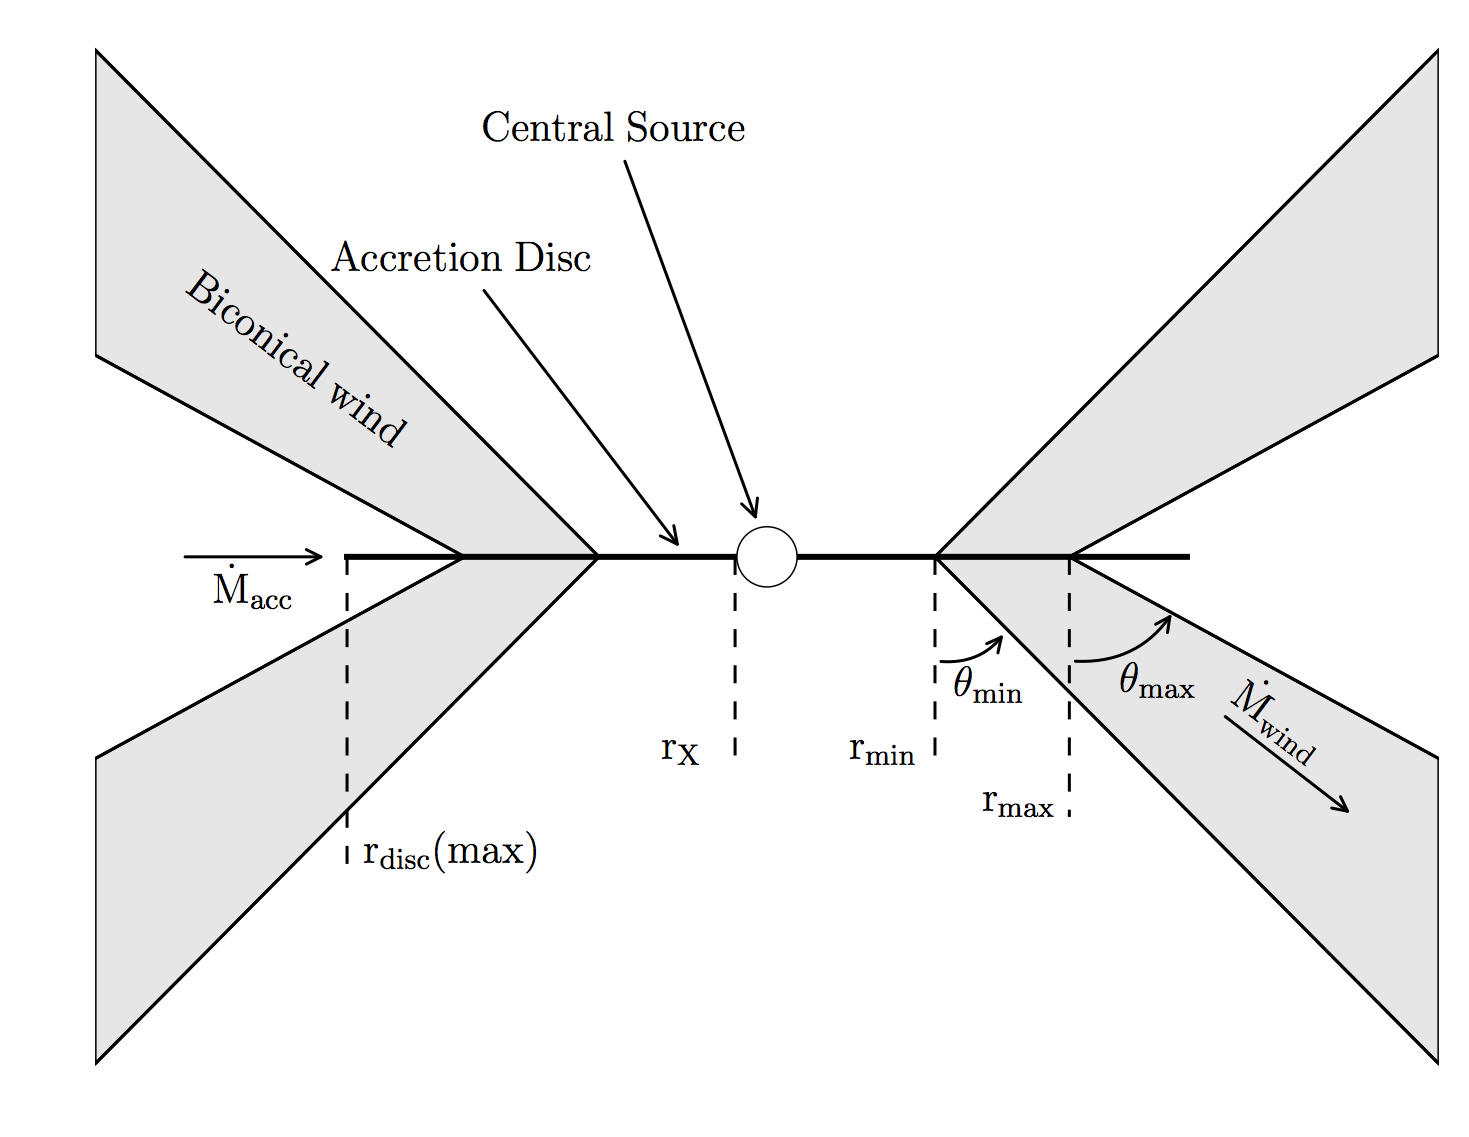
\includegraphics[width=1.0\textwidth]{figures/06-agnpaper/fig1.png}
\caption
[A cartoon showing the geometry and some key parameters of
our biconical quasar wind model.]
{
A cartoon showing the geometry and some key parameters of
our biconical wind model.
}
\label{fig:cartoon}
\end{figure} 

\subsection{Photon Sources}
\label{sec:photon_sources}

We include two sources of r-packets in our model:
An accretion disc and a central X-ray source.
The accretion disc is assumed to be geometrically thin, but optically thick.
Accordingly, the disc is modelled as an ensemble of blackbodies with a 
\cite{shakurasunyaev1973} effective temperature profile. 
The emergent SED is then determined by the specified accretion rate ($\dot{m}$)
and central BH mass ($M_{BH}$).
All photon sources in our model are opaque, meaning
that r-packets that strike them are destroyed.
The inner radius of the disc extends to the innermost 
stable circular orbit (ISCO) of the BH. 
We assume a Schwarzchild BH with an ISCO at $6~r_G$, where 
$r_G = GM_{BH}/c^2$ is the gravitational radius.
For a $10^9~M_\odot$ BH, this is equal to $8.85\times10^{14}~{\rm cm}$ 
or $\sim10^{-4}~{\rm pc}$.  


The X-ray source is treated as an isotropic sphere at the ISCO,
which emits $r$-packets according to a power law in flux with index $\alpha_X$, of the form
\begin{equation}
F_X (\nu) = K_X \nu^{\alpha_X}.
\end{equation}
The normalisation, $K_X$ of this power law is such that it 
produces the specified 2-10~keV luminosity, $L_X$.
The input spectrum for our simulations is therefore a simple combination
of a power law X-ray component and accretion disc spectrum; an example input
spectrum is shown in Fig.~\ref{fig:qso_model_sed}. In actual fact, this
spectrum will be angle dependent due to the geometry of the system and 
the angular emissivity profile of the accretion disc (see sections~\ref{sec:xray}
and \ref{sec:ew_in_model}.
Photons, or $r$-packets, produced by the accretion disc and central X-ray source
are reprocessed by the wind. This reprocessing is dealt with by enforcing strict
radiative equilibrium ({\em modulo} adiabatic cooling; see section~2.3)
via an indivisible energy packet constraint (see Lucy 2002, M15).  

\begin{figure} 
\centering
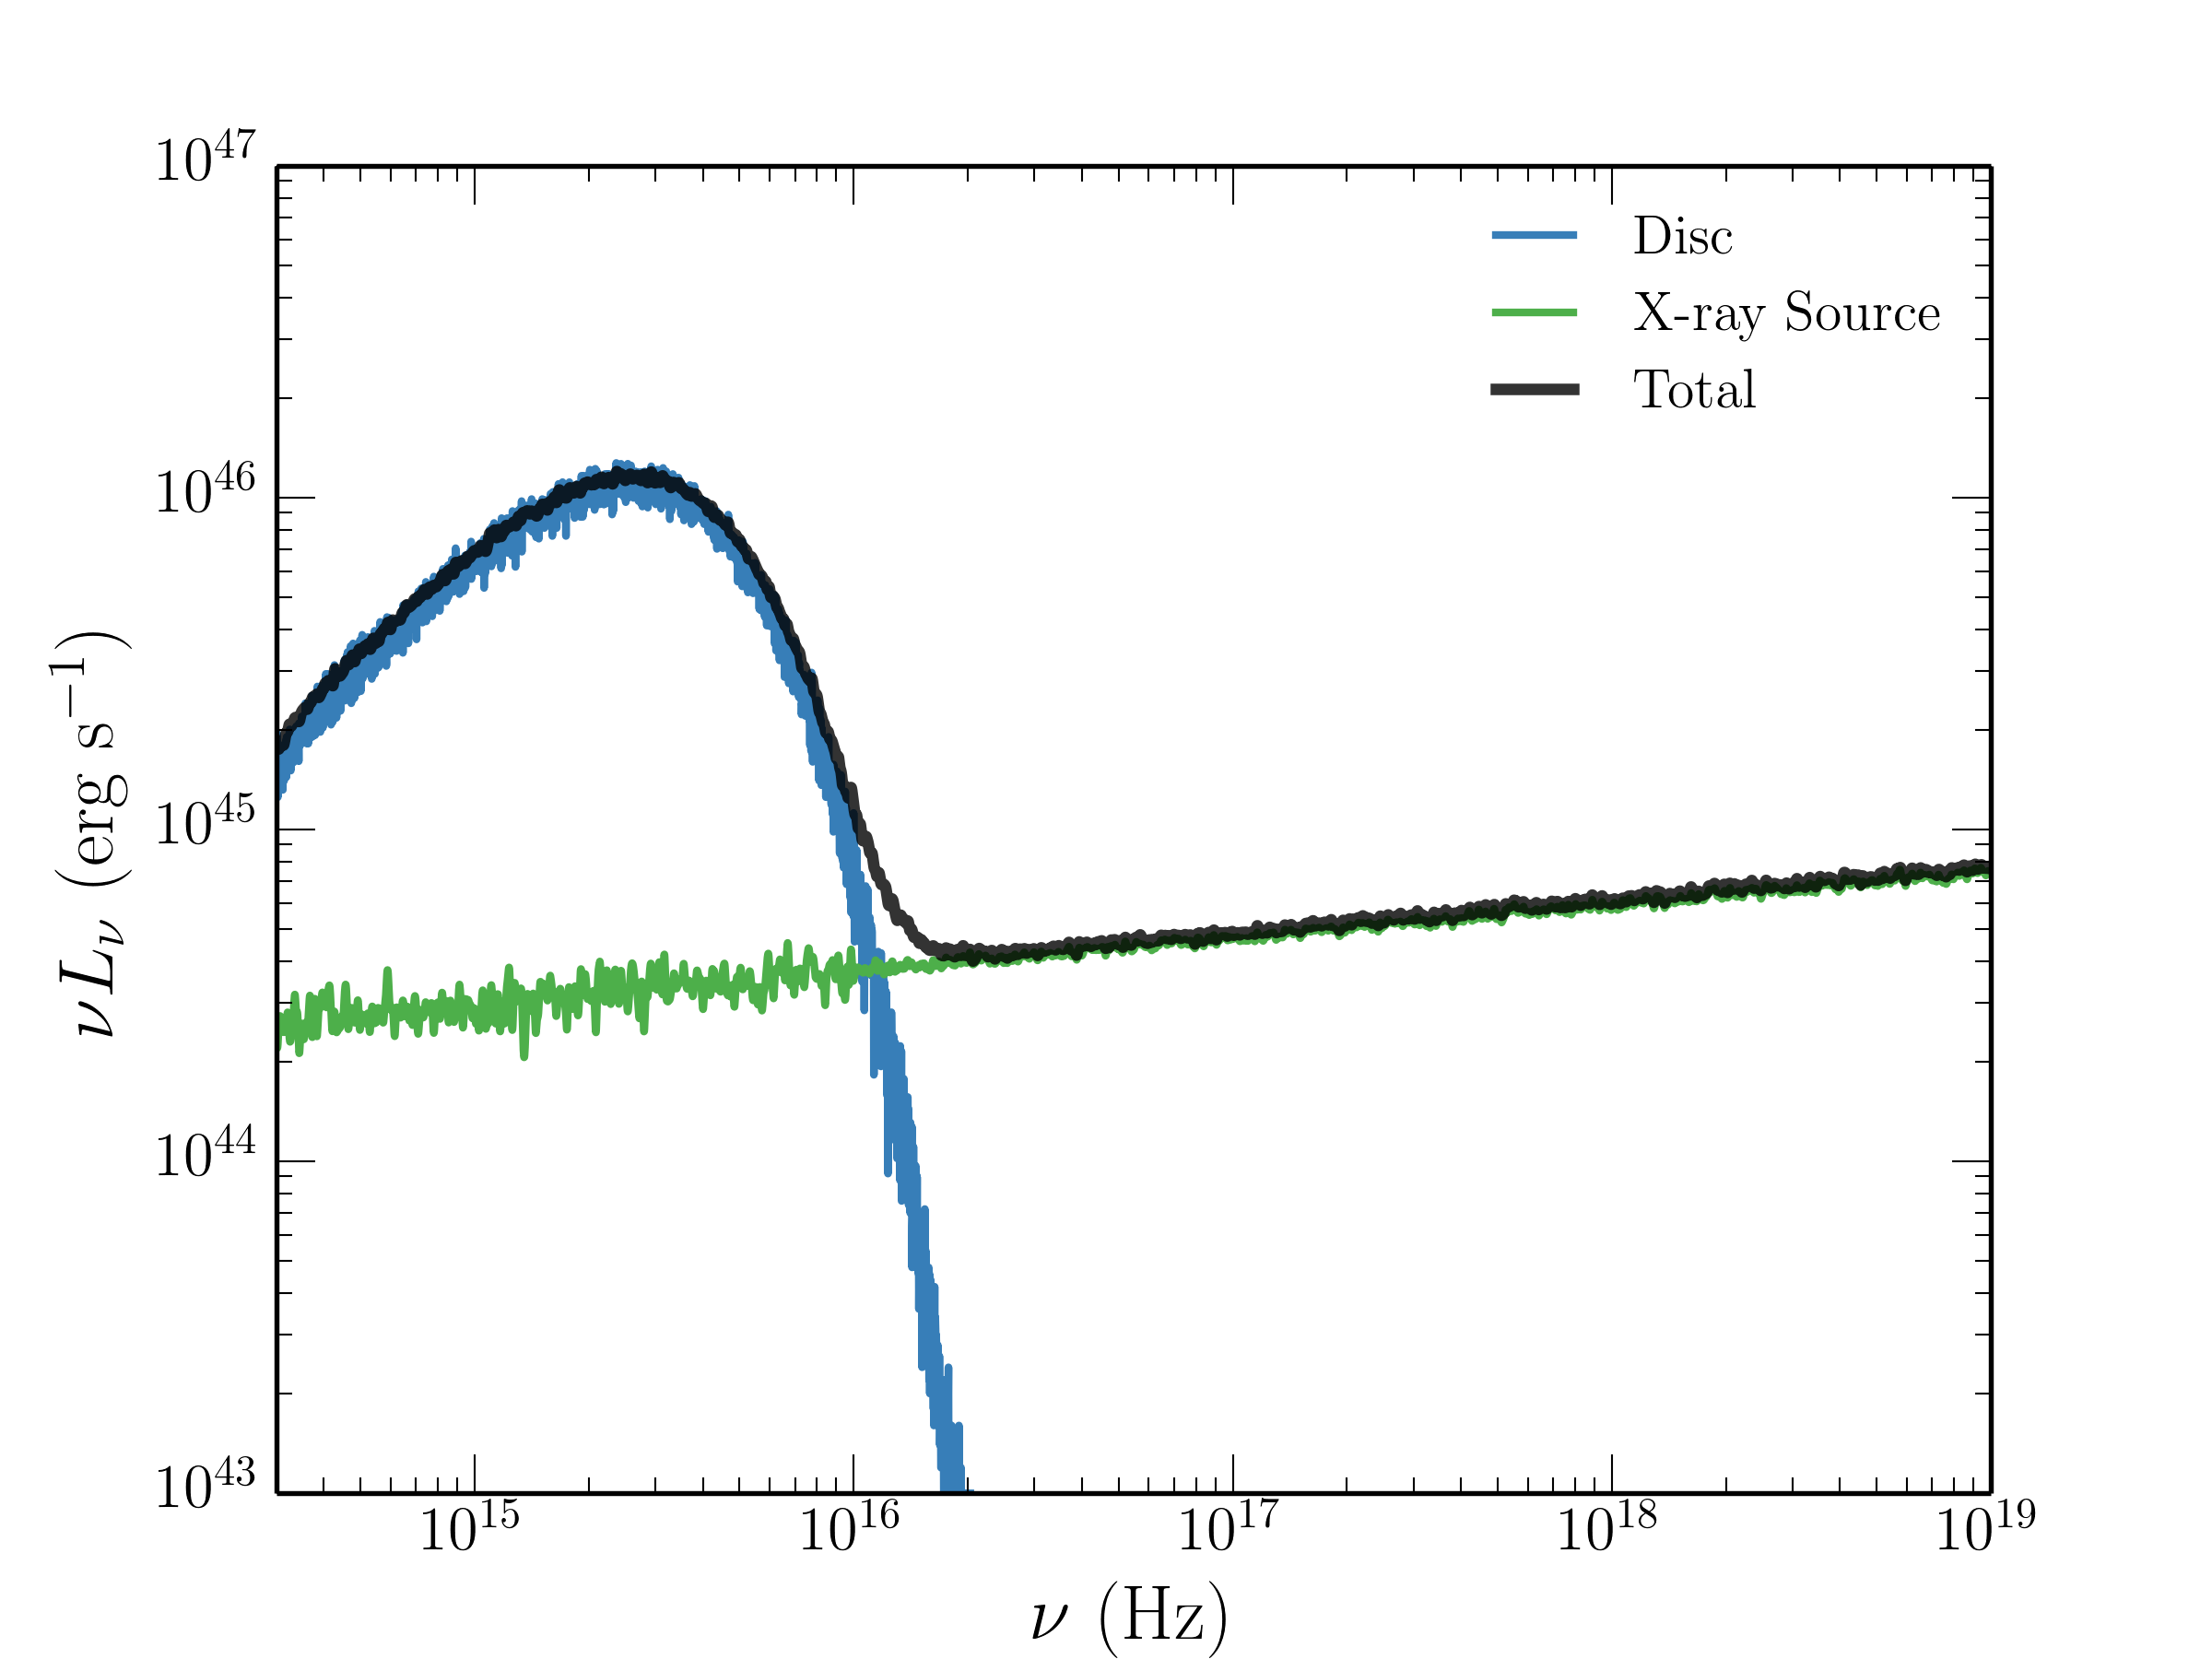
\includegraphics[width=1.0\textwidth]{figures/06-agnpaper/qso_model_sed.png}
\caption
[The input spectrum used for our quasar modelling.]
{
The input spectrum used for our quasar modelling.
}
\label{fig:qso_model_sed}
\end{figure} 

% \subsection{Kinematics and Geometry}

% In the SV93 model, a biconical disc wind rises from the accretion 
% disc between launch radii $r_{min}$ and $r_{max}$.
% The opening angles of the wind are set to $\theta_{min}$ and $\theta_{max}$.
% The poloidal velocity along each individual streamline at a poloidal distance $l$ 
% is then given by
% \begin{equation}
% v_l=v_0+\left[v_{\infty}(r_0)-v_0\right]\frac{\left(l/R_v\right)^{\alpha}}{\left(l/R_v\right)^{\alpha}+1},
% \label{v_law}
% \end{equation}
% where $v_0$ is the velocity at the base of the streamline, $\alpha$ is
% an exponent governing how quickly the wind accelerations and 
% $R_v$ is the `acceleration length', defined as the distance at which
% the outflow reaches half of its terminal velocity, $v_{\infty}$.
% The terminal velocity is set to a fixed multiple of the escape
% velocity, $v_{esc}$, at the base of the streamline (radius $r_0$).
% The rotational velocity, $v_{\phi}$, is initially Keplerian ($v_k = [GM/r_0]^{1/2}$),
% and the wind conserves specific angular momentum, such that 
% \begin{equation}
% v_{\phi} r = v_k r_0.
% \label{v_law}
% \end{equation}
% The velocity law is crucial in determining the output spectra,
% as it affects not only the projected velocities along the line of sight,
% but also the density and ionization state of the outflow.
% A wind that accelerates more slowly will have a denser wind base
% with correspondingly different ionization and emission characteristics.

\subsection{A Simple Approximation for Clumping}

In previous modelling efforts with \py, a smooth outflow was assumed, 
such that the density at a given point was determined only by the 
kinematic parameters and mass loss rate. However, as already discussed,
AGN winds exhibit significant substructure -- the outflow is expected to be
{\em clumpy}, rather than smooth, and probably on a variety of scales. 
A clumpy outflow offers a possible solution to the so-called `over-ionization problem' in 
quasar and AGN outflows \citep[e.g.][]{junk1983,weymann1985,hamann2013}. 
This is the main motivation for incorporating clumping into our model.

Deciding on how to implement clumping into our existing wind models was not straightforward.
First, and most importantly, the physical scale lengths and density contrasts in AGN outflows are not well-constrained from observations or theory.  As a result, while one could envision in principle, clouds with a variety of sizes and density contrasts varying perhaps as function of radius, there would have been very little guidance on how to set nominal values of the various parameters of such a model.
Second, there are significant computational difficulties associated with adequately resolving and realistically modelling a series of small scale, high density regions with a MCRT
-- or for that matter, a hydrodynamical -- code. 
Given the lack of knowledge about the actual type of clumping, I have implemented
a simple approximation used successfully in stellar wind modelling, known as 
{\em microclumping} \citep[e.g.][]{hamann1998,hilliermiller1999,hamann2008}.  

The underlying assumption of microclumping is that clump sizes 
are much smaller than the 
typical photon mean free path, and thus the clumps are 
both geometrically and optically thin. This approach 
allows one to treat clumps only in terms of their volume filling factor, $f_V$, 
instead of having to specify separately their size and density distributions.
In our model, $f_V$ is independent of position (see section~4.4).
The inter-clump medium is modeled as a vacuum,
although the outflow is still non-porous and axisymmetric.
This approach therefore assumes that the inter-clump medium
is unimportant in determing the output spectrum, which
is expected to be true only when density constrasts are large and
the inter-clump medium is both very ionized and of low emissivity and opacity.
The density of the clumps is multiplied by the ``density enhancement'' 
$D=1/f_V$. Opacities, $\kappa$, and emissivities, $\epsilon$, 
can then be expressed as 
\begin{equation}
\kappa = f_V \kappa_C(D);~~\epsilon = f_V \epsilon_C(D).
\end{equation}
Here the subscript $C$ denotes that the quantity is calculated using the 
enhanced density in the clump. The resultant effect is that, {\em for fixed temperature},
processes that are linear in density, such as electron scattering, are unchanged, 
as $f_V$ and $D$ will cancel out. However, any quantity that scales with the square of density, 
such as collisional excitation or recombination, will increase by a factor of $D$.
In our models, the temperature is not fixed, and is instead set by balancing heating and 
cooling in a given cell. In the presence of an X-ray source, this thermal balance is 
generally dominated by bound-free heating and line cooling. The main effect of including 
clumping in our modelling is that it moderates the ionization state due to the increased 
density. This allows an increase in the ionizing luminosity, amplifying the amount of
bound-free heating and also increasing the competing line cooling term
(thermal line emission).

The shortest length scale in a Sobolev MCRT treatment such as ours 
is normally the Sobolev length, given by
\begin{equation}
l_S = \frac{v_{th}}{| dv/ds |}
\end{equation}
This is typically $\sim10^{13}$~cm near the disc plane, increasing outwards.
The Sobolev length is shown, together with the size of the cell
and Thomson mean free path, in Fig.~\ref{fig:length_scales}.
We use the mean density to calculate the Sobolev optical depth, which assumes that
$l_S$ is greater than the typical clump size.
Thus for the microclumping assumption to be formally correct, 
clumps should be no larger than $\sim10^{12}$~cm.
This size scale is not unreasonable for quasar outflows, as
\cite{dekool1995} suggest that BAL flows may have low filling factors with
clump sizes of $\sim10^{11}$~cm.
% An additional concern with this approach to clumping is that the clumps
% may rapidly cool and expand into the inter-clump medium. This is a well-known
% issue in BLR and outflow models (REFs), and requires some kind of confining mechanism,
% such as magnetic confinement \cite[e.g.][]{dekool1995}. Alternatively, as already discussed,
% the LDI may cause clumpy flows as expected in stellar winds.}
\begin{figure} 
\centering
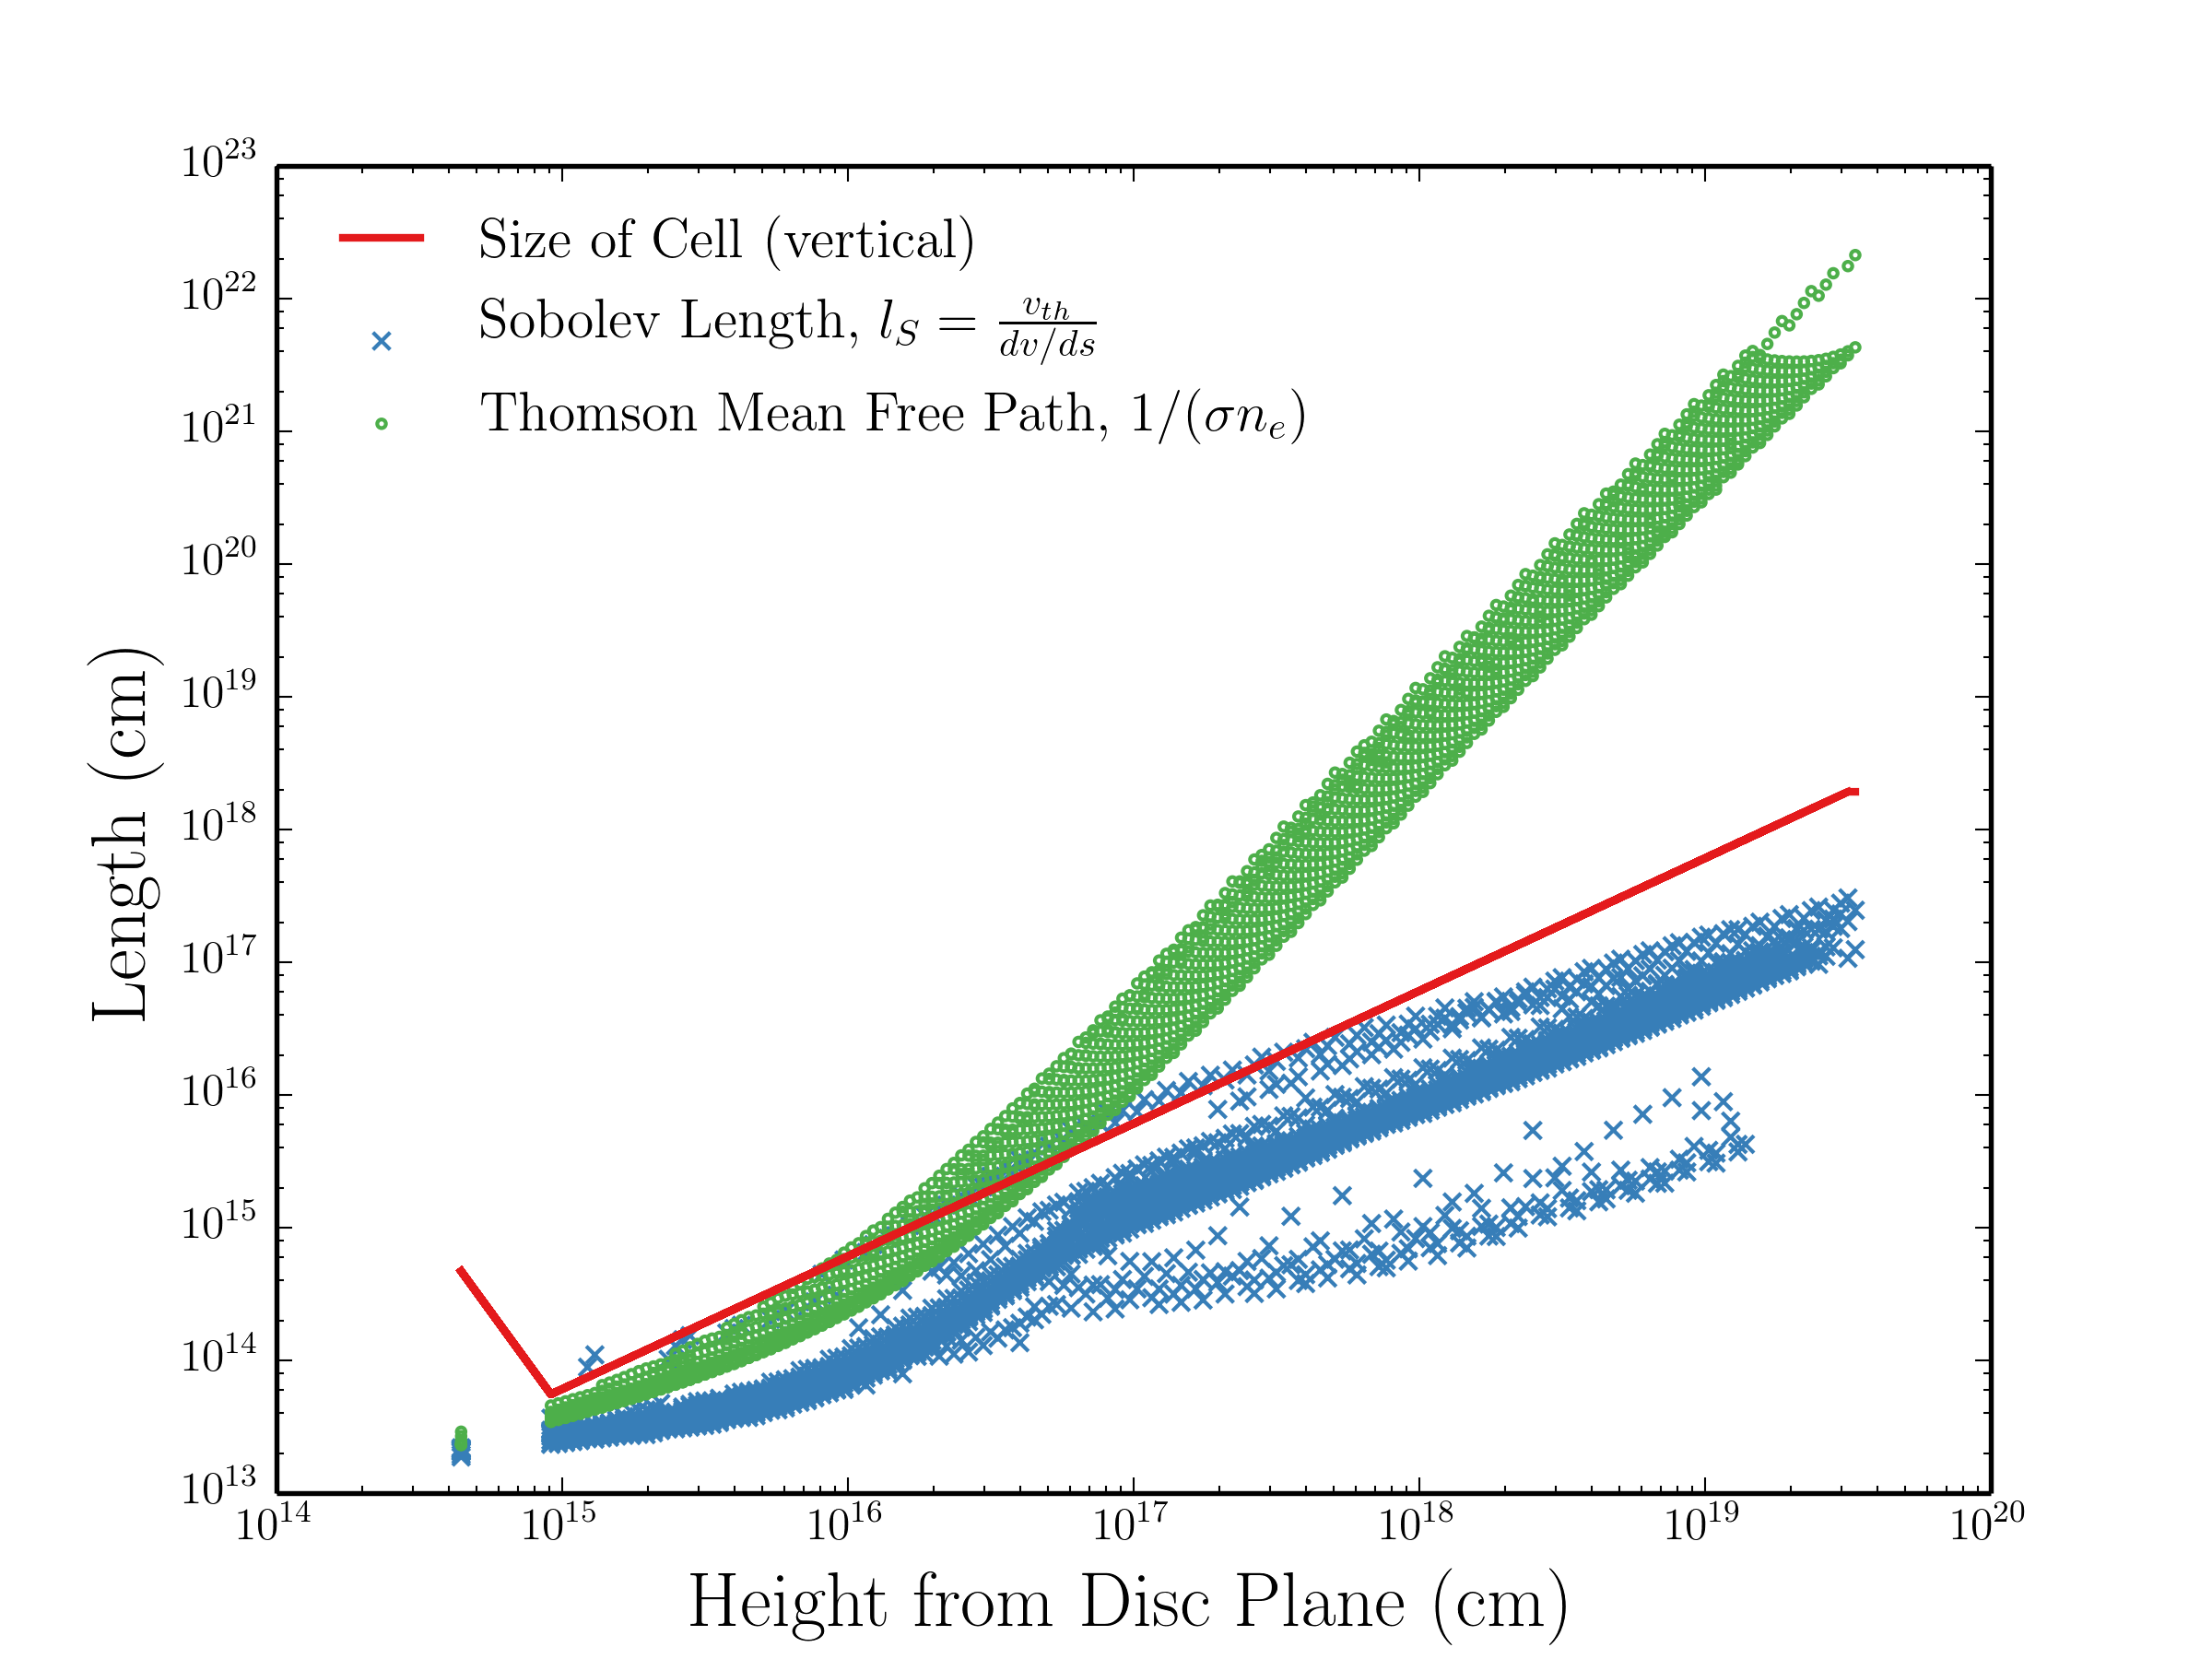
\includegraphics[width=1.0\textwidth]{figures/06-agnpaper/size_of_clumps.png}
\caption
[Some typical length scales for the fiducial model.]
{
Some typical length scales for the fiducial model. 
This places a formal limit of $\sim10^{12}$~cm on clump sizes 
in the microclumping framework, and confirms that the cells are sufficiently
larger than the Sobolev length in almost all cases.
}
\label{fig:length_scales}
\end{figure} 

Our clumping treatment is necessarily simple; it does not adequately
represent the complex substructures and stratifications in ionization
state expected in AGN outflows. 
Nevertheless, this parameterization 
allows simple estimates of the effect clumping has on the ionization 
state and emergent line emission.


\subsection{The Simulation Grid}

Using this prescription, I conducted a limited parameter
search over a 5-dimensional parameter space involving the 
variables $r_{min}$, $\theta_{min}$, $f_V$, $\alpha$ and $R_v$.
The grid points are shown in Table 1.
The aim here was to first fix $M_{BH}$ and $\dot{m}$ to their H13 values,
and increase $L_X$ to $10^{45}$~erg~s$^{-1}$ (a more realistic value for a 
quasar of $10^9M_\odot$ and an Eddington fraction of $0.2$; see section~\ref{sec:xray}).

These models were then evaluated based on 
how closely their synthetic spectra reproduced the 
following properties of quasars and BALQSOs:

\begin{itemize}
\item UV absorption lines 
with $BI > 0$ at $\sim20\%$ of viewing angles (e.g. Knigge et al. 2010);
\item Line emission emerging at low inclinations, with $EW\sim40$\AA in \civline\ \citep[e.g. ][]{shen2011};
\item H recombination lines with $EW\sim50$\AA\ in \la\ \citep[e.g. ][]{shen2011};
\item  \mg\ and \al\ (LoBAL) absorption features with $BI > 0$ at a subset of 
BAL viewing angles;
\item Verisimilitude with quasar composite spectra.
\end{itemize}
Here $BI$ is the `Balnicity Index' (Weymann et al. 1991), given by
\begin{equation}
BI = \int^{25000~{\rm km~s}^{-1}}_{3000~{\rm km~s}^{-1}} C \left( 1 - \frac{f(v)}{0.9} \right) dv.
\end{equation}
The constant $C=0$ everywhere, unless the normalized flux
has satisfied $f(v)<0.9$ continuously for at least $2000$~km~s$^{−1}$, 
whereby $C$ is set to $1$.

In the next section, O present one of the most promising models,
which I refer to as the fiducial model, and discuss
the various successes and failures with respect to the above criteria.
This allows us to gain insight into fundamental geometrical 
and physical constraints and assess the potential for unification. 
We then discuss the sensitivity to key parameters in section~\ref{sec:param_sens}.
The full grid, including output synthetic spectra and plots can be found at
\url{jhmatthews.github.io/quasar-wind-grid/}.

\begin{table}
\centering
\begin{tabular}{p{2cm}p{1cm}p{1cm}p{1cm}p{1cm}}
Parameter & \multicolumn{4}{l}{Grid Point Values}  \\
\hline \hline 
$r_{min}$ 	&	 $60r_{g}$ & $180r_{g}$ & \multicolumn{2}{l}{$300r_{g}$} \\ 
$\theta_{min}$ 	& $55^{\circ}$ & \multicolumn{3}{l}{$70^{\circ}$} \\ 
$R_v$  	        &	 $10^{18}$cm & \multicolumn{3}{l}{$10^{19}$cm} \\ 
$\alpha$ 	&	 $0.5$ & $0.6$ & $0.75$ & $1.5$ \\
$f_V$ 	&	 $0.01$ & \multicolumn{3}{l}{$0.1$}  \\
\hline 
\end{tabular}
\caption
[The grid points used in the parameter search for quasar wind models]
{The grid points used in the parameter search.
The sensitivity to some of these parameters is discussed 
further in section~\ref{sec:param_sens}}
\label{grid_table}
\end{table}



%%%%%%%%%%%%%%%%%%%%%%%%%%%%%%%%%%%%%%%%%%%%%%%%%

% RESULTS

%%%%%%%%%%%%%%%%%%%%%%%%%%%%%%%%%%%%%%%%%%%%%%%%%


\section{Results and Analysis From A Fiducial Model}
\label{sec:qso_results}
Here I describe the results from a fiducial model,
and discuss these results in the context of the criteria 
presented in section 3.4. The parameters of this model are shown in Table~2.
Parameters differing from the benchmark model of H13 are 
highlighted with an asterisk. In this section, I examine the physical 
conditions of the flow, and present the synthetic spectra, before comparing
the X-ray properties of this particular model to samples of
quasars and luminous AGN. 

\begin{table}
\centering
\begin{tabular}{p{3cm}p{4cm}}
\hline Fiducial Model Parameters 	&	 Value \\ 
\hline \hline 
$M_{BH}$ 	 &	 $1\times 10^9~\rm{M_{\odot}}$ \\ 
$\dot{m}_{acc}$ 	 &	 $5~M_{\odot}yr^{-1} \simeq 0.2~\dot{M}_{Edd}$\\ 
$\alpha_X$ 	 &	 $-0.9$ \\ 
$L_{X} $ 	 &	 $10^{45}~\rm{erg~s^{-1}}$$^*$ \\ 
$r_{disc}(min)=r_{X}$   &	 $6r_g=8.8\times10^{14}~{\rm cm}$ \\ 
$r_{disc}(max)$   &	 $3400r_g = 5\times10^{17}~{\rm cm}$ \\ 
$\dot{m}_{wind}$  &	 $5~M_{\odot}yr^{-1}$ \\ 
$r_{min}$ 	&	 $300r_{g} = 4.4\times10^{16}~{\rm cm}$\\ 
$r_{max}$ 	&	 $600r_{g} = 8.8\times10^{16}~{\rm cm}$ \\ 
$\theta_{min}$ 	&	 $70.0^{\circ}$ \\ 
$\theta_{max}$ 	&	 $82.0^{\circ}$ \\ 
%%$\lambda$ 	&	 $0$ \\ 
$v_{\infty}(r_0)$ 	&	 $v_{esc}(r_0)$ \\ 
$R_v$  	        &	 $10^{19}$cm$^*$ \\ 
$\alpha$ 	&	 $0.5^*$ \\
$f_V$ 	&	 $0.01^*$  \\
$n_x$ 	&	 $100$  \\
$n_z$ 	&	 $200$  \\
\end{tabular}
\caption
[Model parameters for the fiducial quasar model.]
{Wind geometry parameters 
used in the fiducial model, as defined in the text and figure 1.
Parameters differing from the benchmark model of H13 are 
highlighted with an asterisk.}
\label{wind_param}
\end{table}



\subsection{Physical Conditions and Ionization State}


\begin{figure*}
\centering
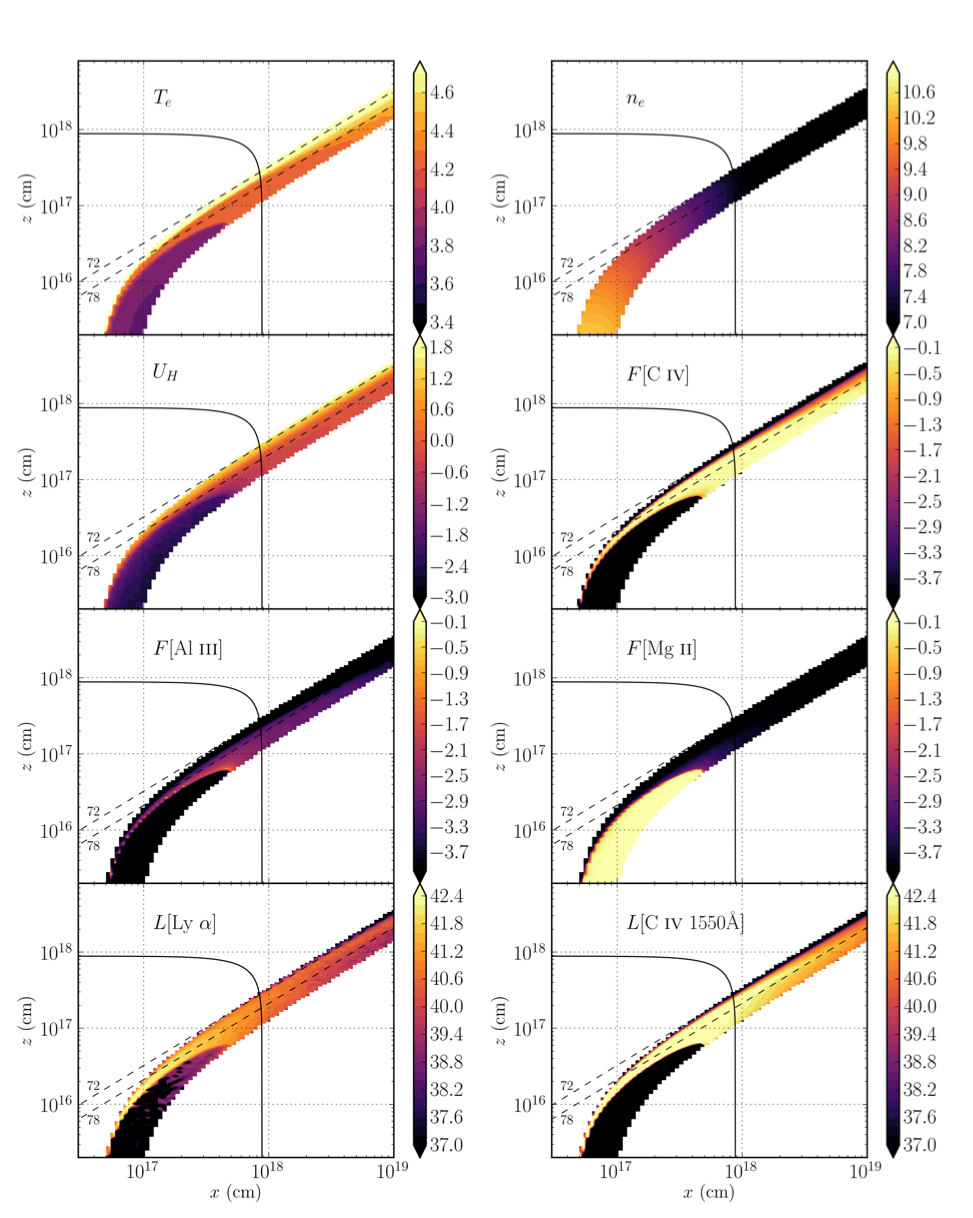
\includegraphics[width=1.0\textwidth]{figures/06-agnpaper/fig2.png}
\caption
[Contour plots showing the logarithm of some important 
physical properties of the quasar outflow.]
{
Contour plots showing the logarithm of some important 
physical properties of the outflow. The spatial scales are
logarithmic and the $x$ and $z$ scales are not the same.
Symbols are defined in the text.
The solid black line marks a sphere at $1000~r_G$.
The dotted lines show the $72^\circ$ and $78^\circ$ sightlines 
to the centre of the system, and illustrate that different sightlines
intersect material of different ionization states.
The line luminosities, $L$, represent the luminosity of photons
escaping the Sobolev region for each line. These photons do not
necessarily escape to infinity.
}
\label{fig:wind}
\end{figure*}

\begin{figure} 
\centering
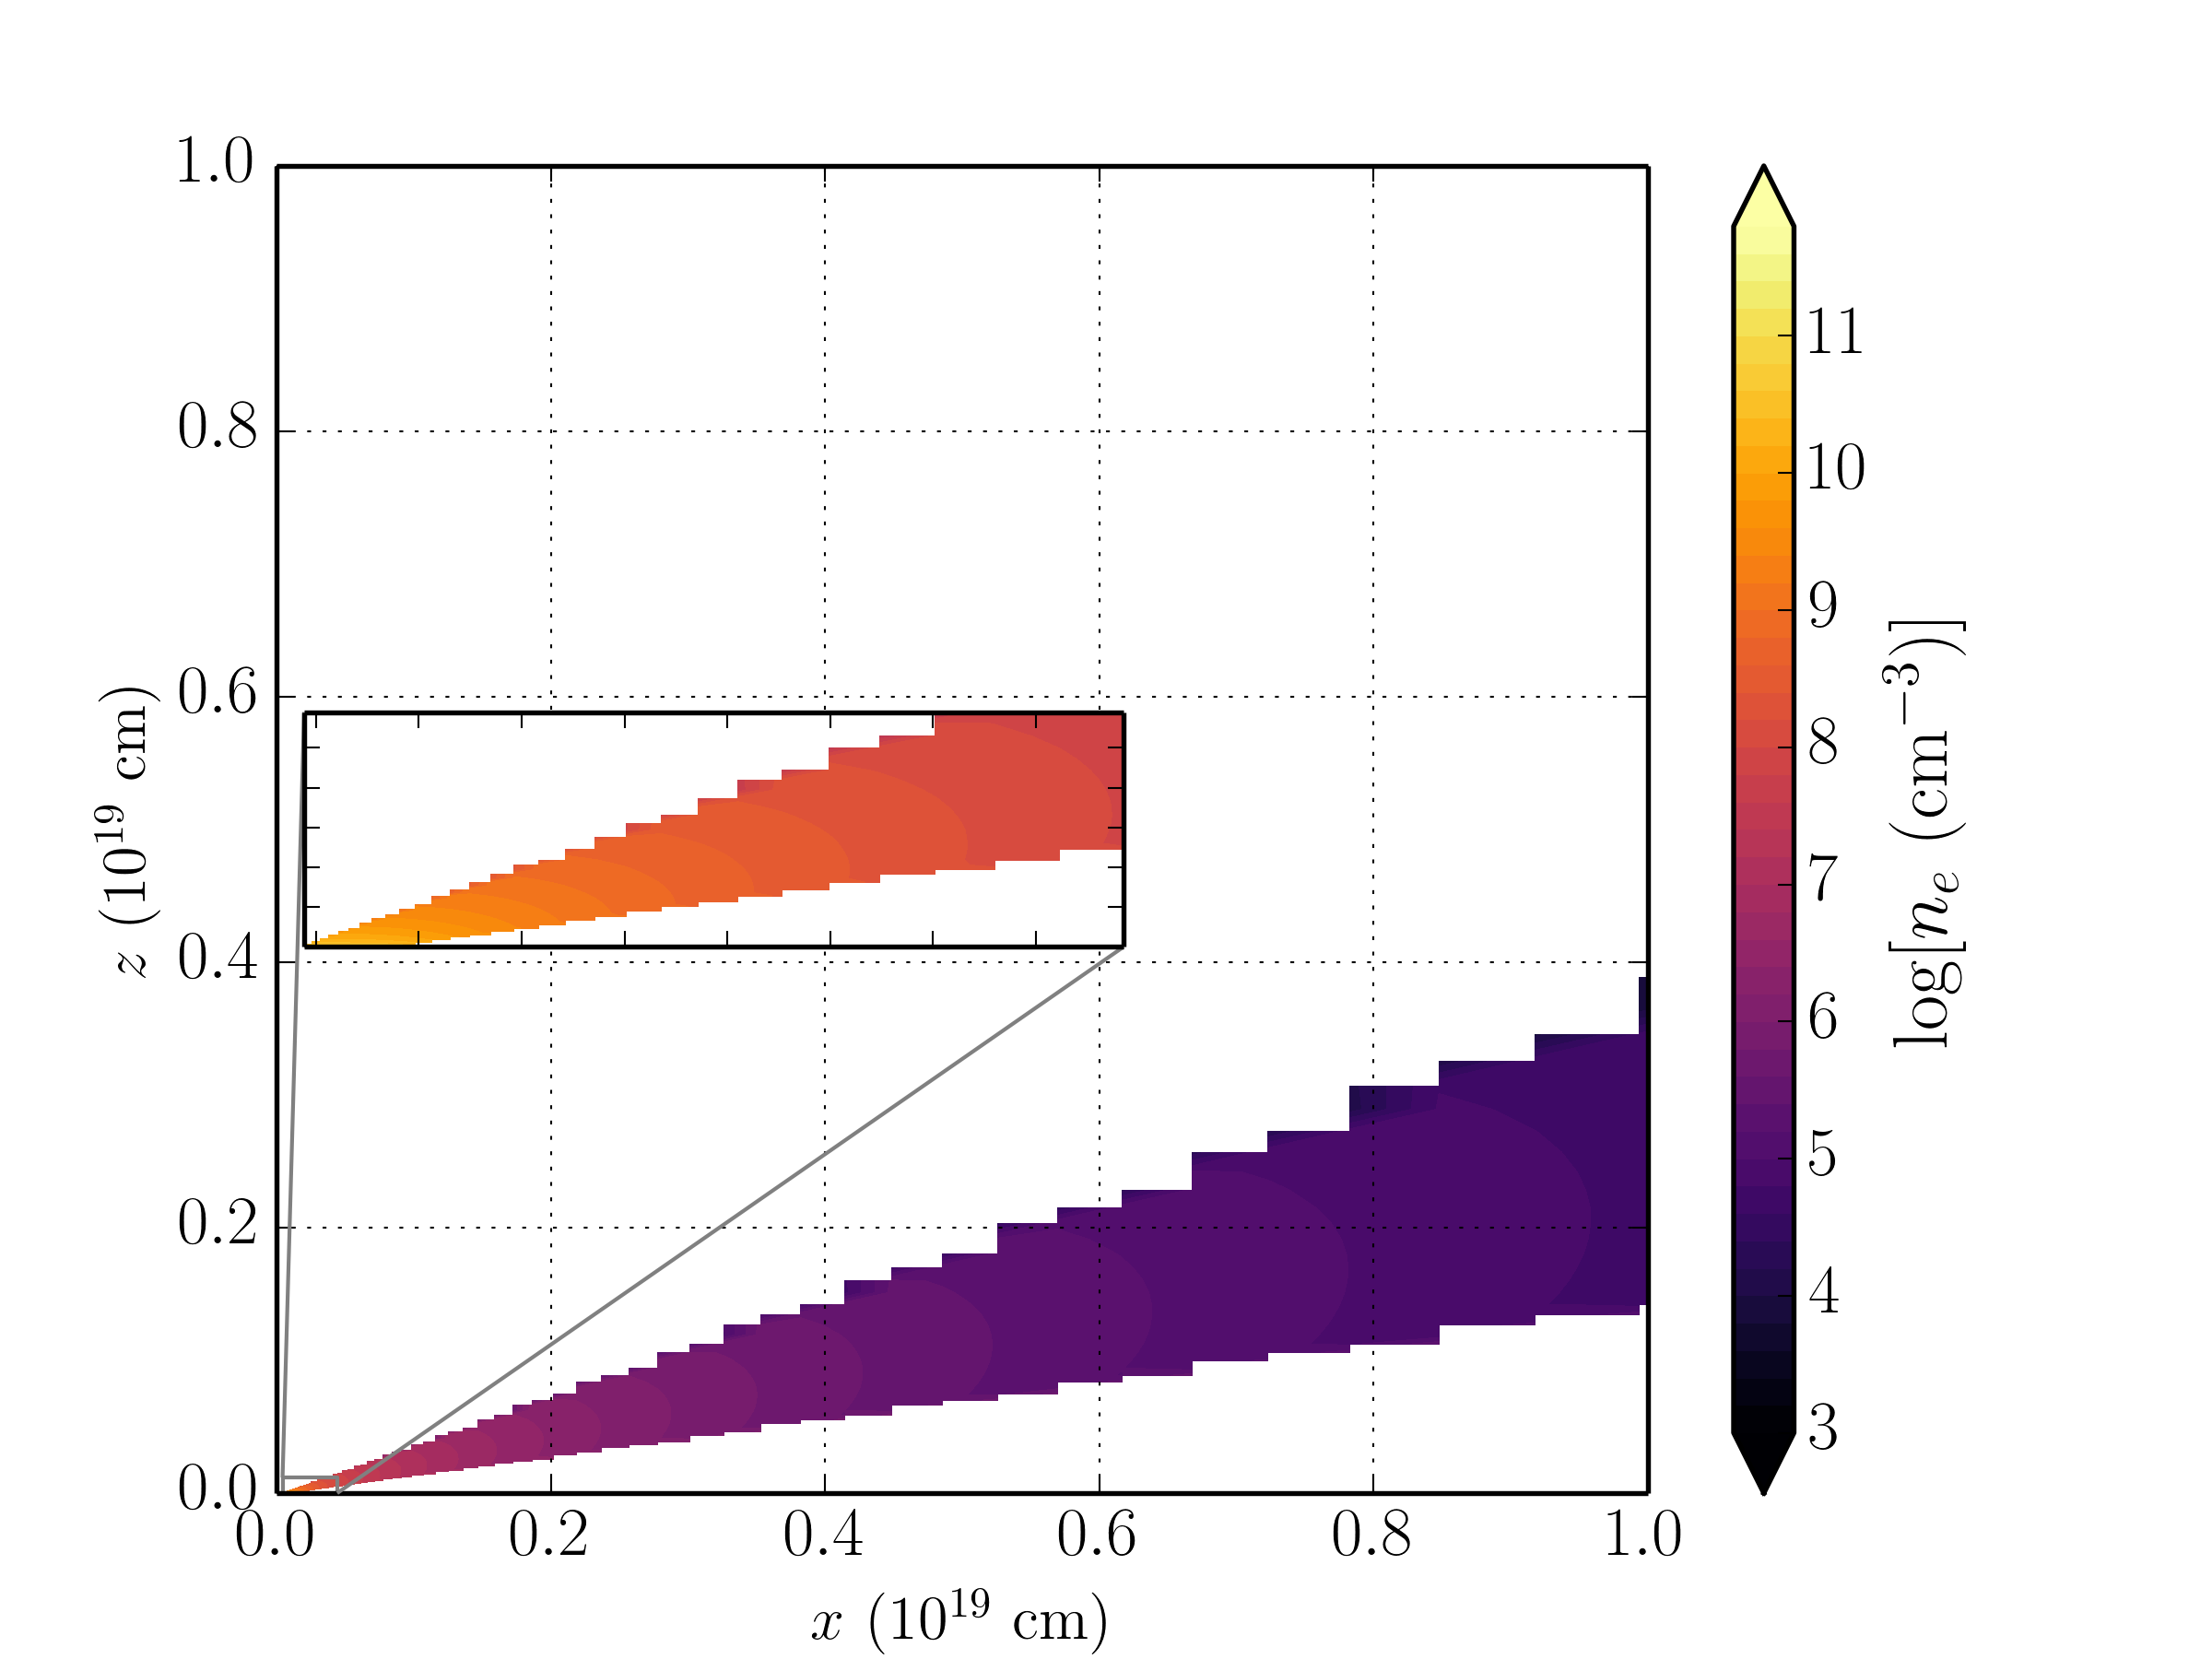
\includegraphics[width=0.8\textwidth]{figures/06-agnpaper/ne_in_wind.png}
\caption
[The electron density in the fiducial model on linear axes.]
{
The electron density in the model, this time on linear axes
in order to illustrate the density contrasts and scale of the system.
The plot is on the scale of the acceleration length, whereas
the inset is a box of $2700 \times 800 r_G$, where the bottom left corner
corresponds to the base of the innermost streamline.
}
\label{fig:ne_in_wind}
\end{figure} 

\noindent
Fig.~\ref{fig:wind} shows the physical properties of the wind.
The wind rises slowly from the disc at first, with densities within clumps
of $n_H \sim 10^{11}~\rm{cm^{-3}}$ close to the disc plane, 
where $n_H$ is the local number density of H. To illustrate the degree
of scale and density ranges in the model I also show $n_e$ in the wind
on a linear scale in Fig.~\ref{fig:ne_in_wind}.
The flow then accelerates over a scale length of $R_V=10^{19}~\rm{cm}$
up to a terminal velocity equal to the escape velocity at the streamline base
($\sim10,000~\rm{km~s^{-1}}$). This gradual acceleration results in
a wind that exhibits a stratified ionization structure, with low ionization material
in the base of the wind giving way to highly ionized plasma further out.
This is illustrated in Fig.~\ref{fig:wind} 
by the panels showing the ion fraction $F=n_j/n_{tot}$ of some important ions.
The clumped wind produces the range of ionization states observed
in quasars and BALQSOs, while adopting a realistic $2-10$ keV X-ray luminosity
of $L_{X}=10^{45}~\rm{erg~s^{-1}}$. Without clumping, this wind would be over-ionized 
to the extent that opacities in e.g., \civ\ would be entirely negligible (see H13).

One common way to quantify the ionization state of a plasma
is through the ionization parameter, $U_H$, given by equation~\ref{eq:ip}.
Shown in Fig.~\ref{fig:wind},
the ionization parameter is a useful measure of the global ionization state,
as it represents the ratio of the number density of 
H ionizing photons to the local H density.
It is, however, a poor representation of the 
ionization state of species such as \civ\ as it encodes no information
about the shape of the SED. In our case, the X-ray photons 
are dominant in the photoionization of the UV resonance line ions. 
This explains why a factor of 100 increase in X-ray luminosity requires
a clumping factor of 0.01, even though the value of $U_H$ decreases by only a factor of $\sim10$ compared to H13. 

The total line luminosity also increases dramatically compared to the unclumped model
described by H13. This is because the denser outflow can absorb the increased
X-ray luminosity without becoming over-ionized, leading to a hot plasma which
produces strong collisionally excited line emission.
This line emission typically emerges on the edge of the wind
nearest the central source. The location of the line emitting regions
is dependent on the ionization state, as well as the incident X-rays.
The radii of these emitting regions is important,
and can be compared to observations. The line luminosities, $L$,
shown in the figure correspond to the luminosity in $\LUM$ of photons
escaping the Sobolev region for each line. 
As shown in Fig.~\ref{fig:wind},
the \civline\ line in the fiducial model is typically formed between 
$100-1000~r_G$ ($\sim10^{17}-10^{18}~\rm{cm}$).
This is in rough agreement with the reverberation mapping 
results of Kaspi (2000) for the $2.6\times10^{9} M_\odot$ quasar S5 0836+71,
and also compares favourably with microlensing measurements of the size of the
\civline\ emission line region in the BALQSO H1413+117 \citep{odowd2015}.


\subsection{Synthetic Spectra: Comparison to Observations}

\begin{figure*}
\centering
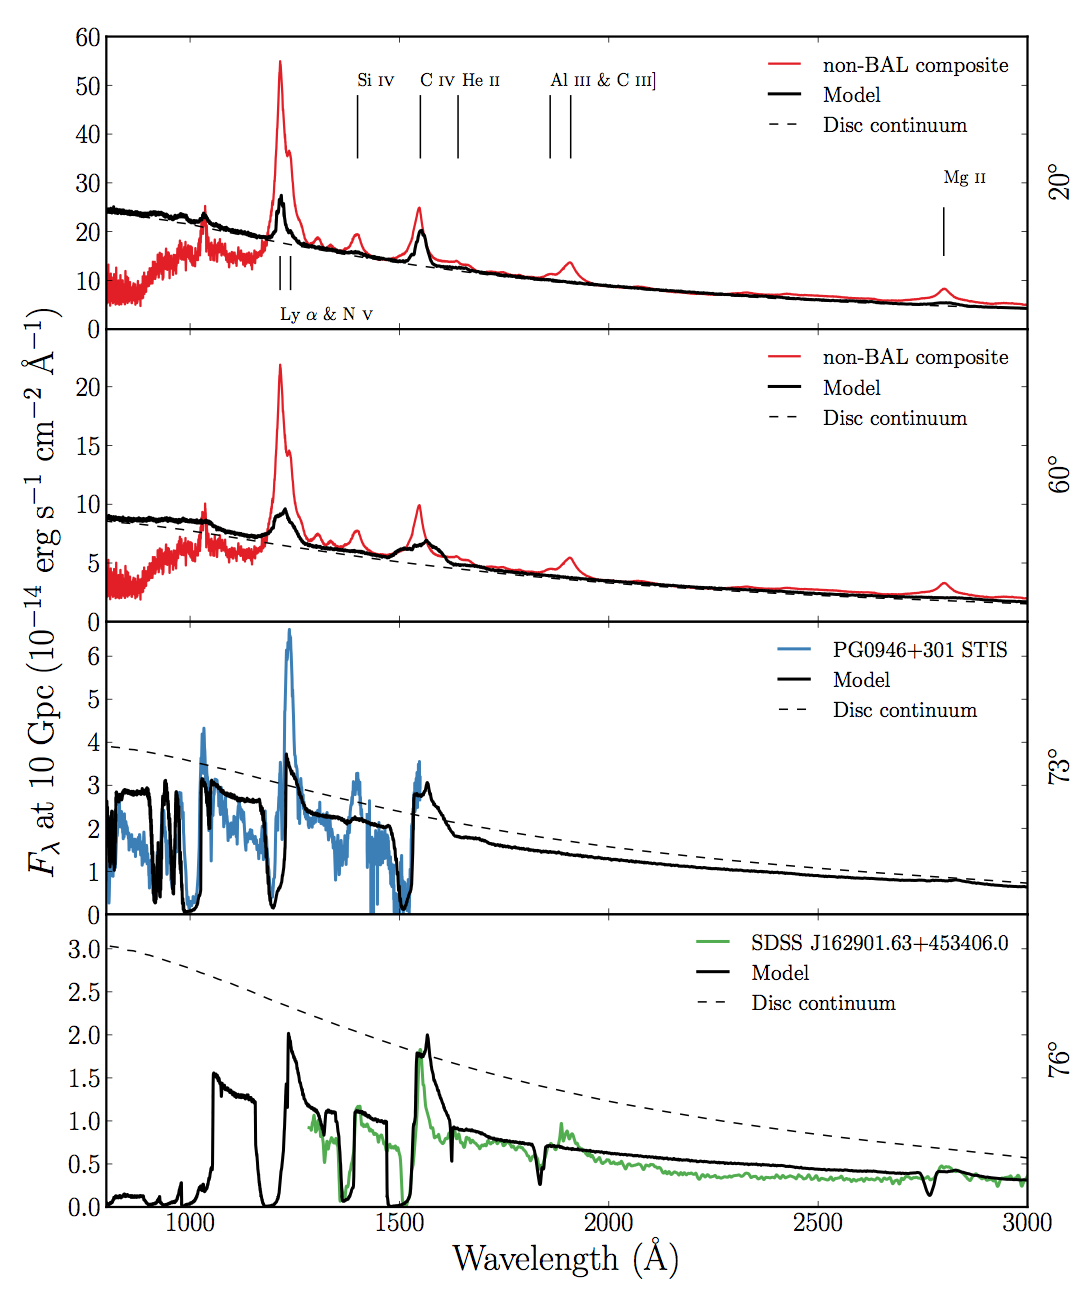
\includegraphics[width=1.0\textwidth]{figures/06-agnpaper/fig3.png}
\caption
[Synthetic spectra at four viewing angles for the fiducial quasar model.]
{
Synthetic spectra at four viewing angles for the fiducial model. At 
$20^\circ$ and $60^\circ$ I show a comparison to an SDSS quasar composite
from Recihard et al. (2003). At $73^\circ$ and $76^\circ$ I show a comparison to
an {\sl HST} STIS spectrum of the high BALnicity BALQSO 
PG0946+301 (Arav et al. 2000), and an SDSS spectrum of the LoBAL quasar 
SDSS J162901.63+453406.0, respectively. The dotted line shows a disc
only continuum to show the effect of the outflow on the continuum level. 
All the spectra are scaled to the model flux at $2000$\AA, expect for the 
{\sl HST} STIS spectrum of PG0946+301, which is scaled to $1350$\AA\
due to the incomplete wavelength coverage.
% HST STIS spectrum of PG0946+301 (Arav et al. 2000)
}
\label{fig:uvspec}
\end{figure*}

\begin{figure} 
\centering
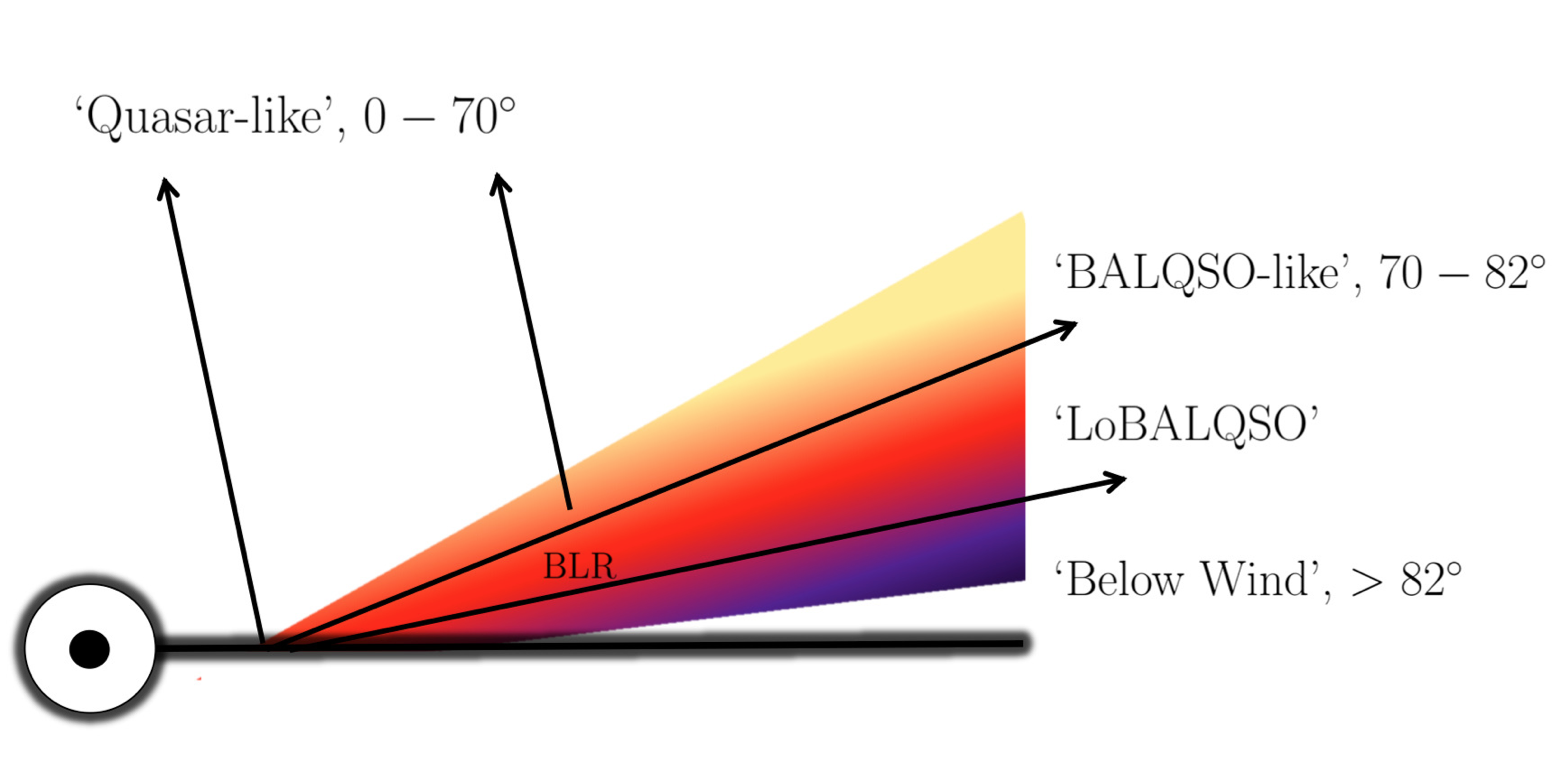
\includegraphics[width=1.0\textwidth]{figures/06-agnpaper/fig4.png}
\caption
[A schematic showing the broad classes of sightline 
in the fiducial model.]
{
A cartoon describing the broad classes of sightline 
in the fiducial model, illustrating how geometric effects lead to 
the different emergent spectra. The colour gradient is approximate,
but indicates the stratified ionization structure, 
from highly ionized (yellow) to low ionization (purple) material.
%[FIGURE NEEDS IMPROVING]
}
\label{fig:sightline}
\end{figure} 

\begin{figure*}
\centering
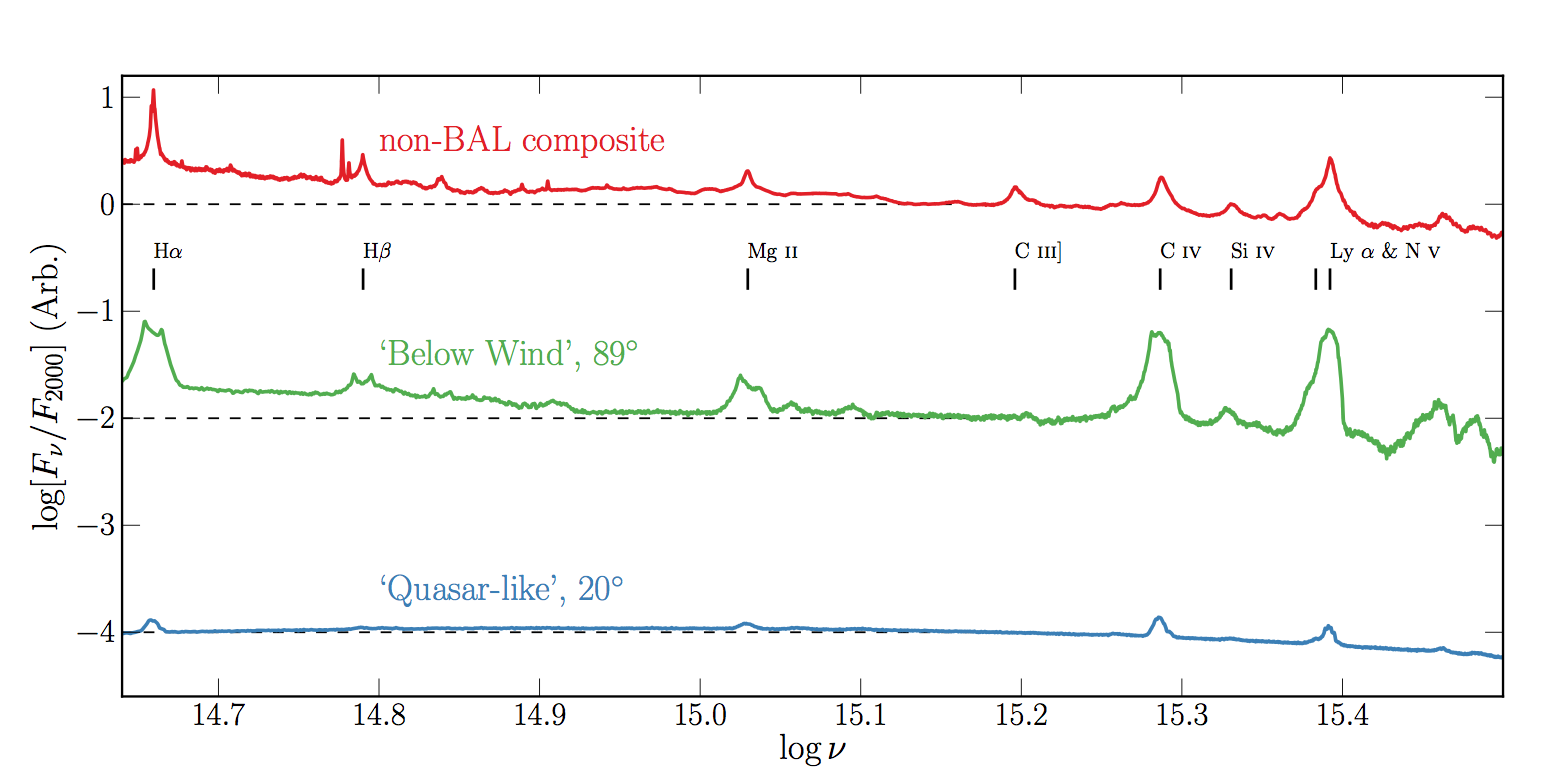
\includegraphics[width=0.9\textheight, angle=270]
{figures/06-agnpaper/fig5.png}
\caption
[Synthetic spectra at two viewing angles compared to the non-BAL SDSS quasar composite.]
{
Synthetic spectra at two viewing angles, 
this time in frequency space and including the optical band,
compared to the non-BAL SDSS quasar composite. The spectra are normalised to the flux at 
$2000$\AA, then an offset of 2 is applied per spectrum for clarity -- the dotted lines show the zero point of $F_\nu / F_{2000}$ in each case.
}
\label{fig:sed}
\end{figure*}

\noindent
Fig.~\ref{fig:uvspec} shows the synthetic spectrum in the UV from the fiducial model. 
To assess the ability of the synthetic spectra to match real 
quasar spectra, I also show {\sl Sloan Digital Sky Survey} (SDSS) quasar
composites from \cite{reichard2003}, normalised to the flux at 2000\AA\
for low inclinations. Unfortunately, the wide variety of
line profile shapes and internal trough structure in BALQSOs
tends to `wash out' BAL troughs in composite spectra
to the extent that BALQSO composites do not resemble typical BALQSOs.
Because of this, I instead compare to a {\sl Hubble Space Telescope} 
STIS spectrum of the high BALnicity BALQSO PG0946+301 (Arav et al. 2000),
and an SDSS spectrum of the LoBAL quasar SDSS J162901.63+453406.0,
for the angles of $73^\circ$ and $76^\circ$, respectively. 
We show a cartoon illustrating how geometric effects determine
the output spectra in Fig.~\ref{fig:sightline}.  

\subsubsection{Broad absorption lines (`BALQSO-like' angles)}
\label{sec:balqso_angles}

The UV spectrum is characterised by strong BAL 
profiles at high inclinations ($> 70^\circ$). 
This highlights the first success of our model: 
clumping allows the correct ionization state 
to be maintained in the presence of strong X-rays, 
resulting in large resonance line opacities. 
At the highest inclinations, the 
cooler, low ionization material at the base of the wind
starts to intersect the line of sight. This produces 
multiple absorption lines in species such as \mg,
\al\ and Fe~\textsc{ii}. The potential links to LoBALQSOs and 
FeLoBALQSOs are discussed in section 2.4.

The high ionization BAL profiles are often saturated, and the location in velocity space
of the strongest absorption in the profile varies with inclination.
At the lowest inclination BAL sight lines, the strongest absorption occurs at the red edge,
whereas at higher inclinations (and for the strongest BALs)
the trough has a sharp edge at the terminal velocity.
This offers one potential explanation for the wide range of BALQSO absorption
line shapes \citep[see e.g.][]{trump2006,knigge2008,filizak2014}.

The absorption profiles seen in BALQSOs are often non-black, but saturated, 
with flat bases to the absorption troughs \citep{arav1999b,arav1999a}.
This is usually explained either as  partial covering of the continuum
source or by scattered contributions to the BAL troughs, necessarily
from an opacity source not co-spatial with the BAL forming region.
The scattered light explanation is supported by spectropolarimetry results
\citep{lamy2000}. Our spectra do not show non-black, saturated profiles.
We find black, saturated troughs at angles $i > 73^\circ$, and the BALs
are non-saturated at lower inclinations. The reasons for this are inherent 
in the construction of our model. 
First, the microclumping assumption does not allow for 
porosity in the wind, meaning that it does not naturally produce
a partial covering absorber. To allow this, an alternative approach
such as {\em macroclumping} would be required \citep[e.g.][]{hamann2008,surlan2012}.
Second, our wind does not have a significant scattering contribution 
along sightlines which do not pass through the BAL region,
meaning that any scattered component to the BAL troughs is absorbed by line opacity.
This suggests that either the scattering cross-section of the wind must
be increased (with higher mass loss rates or covering factors), or 
that an additional source of electron opacity is required, potentially
in a polar direction above the disc. We note the scattering contribution
from plasma in polar regions is significant in some `outflow-from-inflow'
simulations \citep{KP09, simproga2012}.

\subsubsection{Broad emission lines (`quasar-like' angles)}

\begin{table}
\centering
\begin{tabular}{p{2cm}p{2cm}p{3cm}}
\hline Property & Synthetic, $20^\circ$ & Observed  (S11) \\ 
\hline \hline
$\log L$[C~\textsc{iv}]  & $44.60$ & $44.42 \pm 0.32$  \\
$\log L$[Mg~\textsc{ii}] & $43.92$ & $43.54 \pm 0.28$  \\
$\log (\nu L_{\nu})_{1350}$  & $46.42$ & $46.01 \pm 0.30$ \\
$\log (\nu L_{\nu})_{3000}$  & $46.18$ & $45.79 \pm 0.30$ \\
\hline
\end{tabular}
\caption
[Some derived spectral properties of the fiducial model compared to observations.]
{
Some derived spectral properties of the fiducial model, at $20^\circ$,
compared to observations. The observed values are taken from the Shen et al. (2011)
SDSS DR7 Quasar catalog, and correspond to mean values with standard deviations in log space
from a subsample with $8.5>\log(M_{BH})<9.5$ and $1.5<\log (L_{bol}/L_{Edd}) < 0$,
where the BH mass is a \civ\ virial estimate. 
Units are logarithms of values in erg~s$^{-1}$.
%unless stated.otherwise.
}
\label{line_lums}
\end{table}


Unlike H13, significant collisionally excited line emission now emerges
at low inclinations in the synthetic spectra, particular in the \civ\ and \nv\
lines. We also find a strong \la\ line and weak He~\textsc{ii}~$1640$\AA\ line
as a result of our improved treatment of recombination using macro-atoms. 
In the context of unification, this is a promising result, 
and shows that a biconical wind can produce significant 
emission at `quasar-like' angles. To demonstrate this further,
I show line luminosities and monochromatic continuum luminosities
from the synthetic spectra in Table~\ref{line_lums}. These are compared to
mean values from a subsample of the SDSS DR7 quasar catalog \citep{shen2011} 
with BH mass and Eddington fraction estimates similar to the fiducial model values 
(see caption). The spectra do not contain the strong 
C~\textsc{iii}]~1909\AA\ line seen in the quasar composite spectra, 
but this is due to a limitation of our current treatment of C; semi-forbidden
(intercombination) lines are not included in our modelling.

In Fig.~\ref{fig:sed}, I show an $F_{\nu}$ spectrum with broader waveband coverage
that includes the optical, showing that our synthetic spectra 
also exhibit \ha\ and \hb\ emission. 
In this panel, I include a low inclination and 
also a very high inclination 
spectrum, which looks underneath the wind cone. This model shows 
strong line emission with very similar widths and line ratios to the quasar composites, and
the Balmer lines are double peaked, due to velocity projection effects.  
Such double-peaked lines are seen in so-called `disc emitter' systems 
\citep[e.g.][]{eracleous1994} but not the majority of AGN.     
The line equivalent widths (EWs) increase at high inclination
due to a weakened continuum from wind attenuation, 
disc foreshortening and limb darkening. This effect also 
leads to a redder continuum slope, as seen in quasars, which is
due to Balmer continuum and Balmer and Fe~\textsc{ii} line emission.
This extreme $89^\circ$ viewing angle cannot represent a typical quasar within a unified model,
but does show that a model such as this can naturally reproduce quasar emission lines
if the emissivity of the wind is increased {\em with respect to the disc continuum}.
In addition, it neatly demonstrates how a stratified outflow can naturally
reproduce the range of ionization states seen in quasars. 

Despite a number of successes, 
there are a some properties of the synthetic spectra
that are at odds with the observations. First, the ratios of the 
EW of the \la\ and \mgline\ lines
to the EW of \civline\ are much lower than in the composite spectra. 
Similar problems have also been seen in simpler photoionization models for the 
BLR \citep{netzer1990}.
It may be that a larger region of very dense ($n_e\sim10^{10}$cm$^{-3}$) 
material is needed, which could correspond to a disc atmosphere or 
`transition region' 
\citep[see e.g.][]{MCGV95,knigge1998}. \nocite{knigge1998} 
While modest changes to geometry may permit this, the initial grid search 
did not find a parameter space in which the \la\ or \mg\ EWs
were significantly higher (see section~\ref{sec:param_sens}). 
Second, EWs increase with inclination 
(see Fig.~\ref{fig:uvspec} and Fig.~\ref{fig:sed}; also Fig.~\ref{fig:lobal}).
This is discussed further in section~\ref{sec:ew_in_model}.

\subsection{X-ray Properties}
\label{sec:xray}


\begin{figure*}
\centering
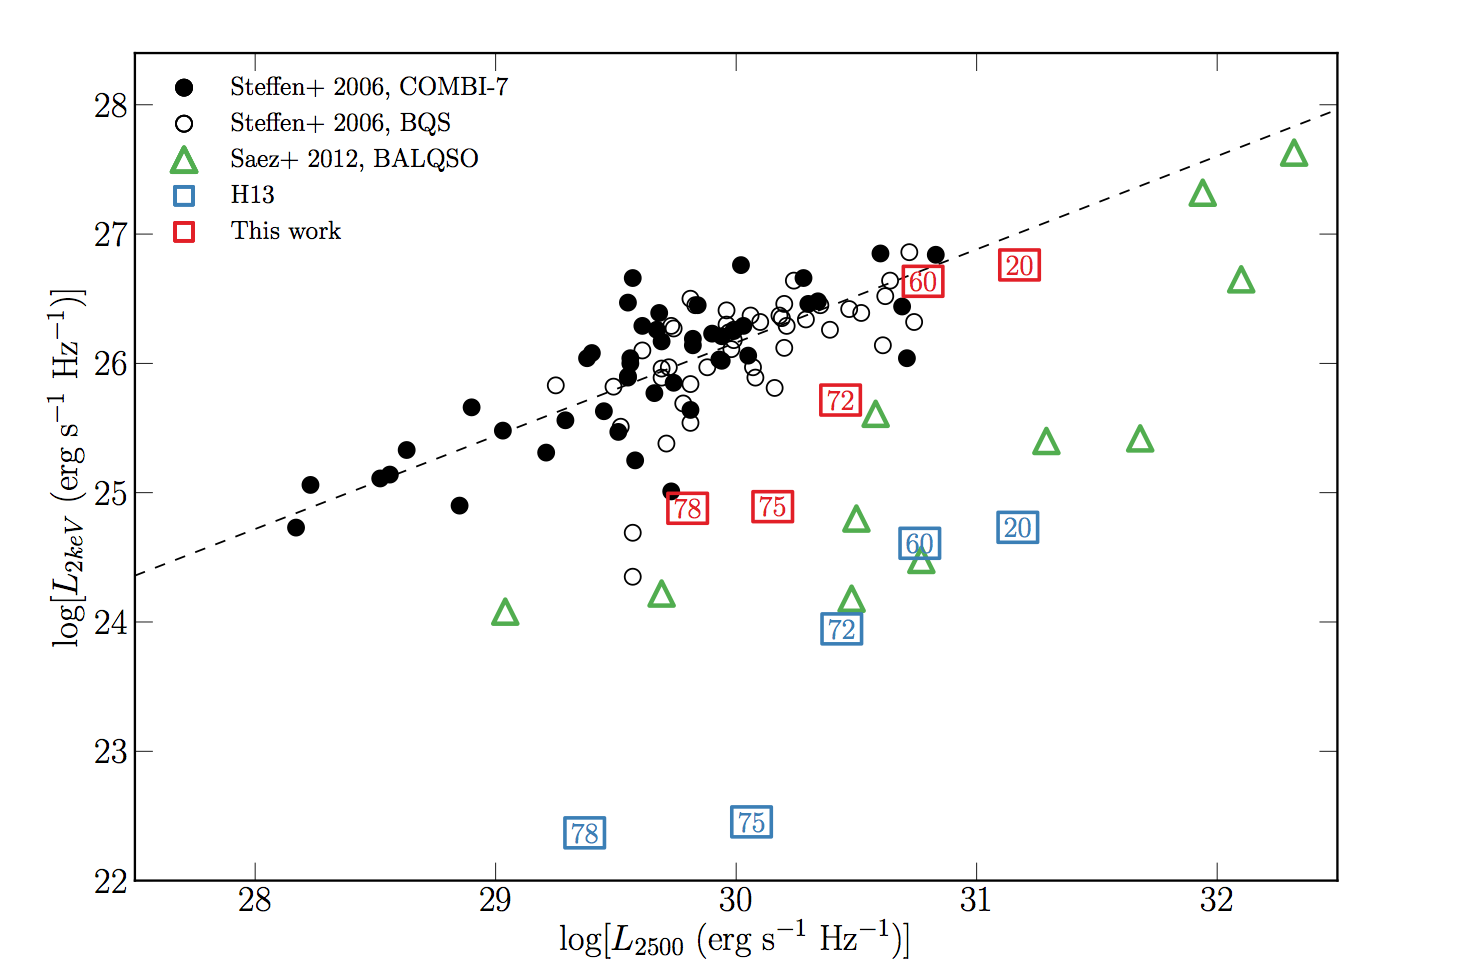
\includegraphics[width=1.0\textwidth]{figures/06-agnpaper/fig6.png}
\caption
[X-ray properties of the clumped quasar model compared to H13 and samples
from the literature.]
{
X-ray ($2$~keV) luminosity of the our clumped model (red squares) 
and the H13 model (blue squares), plotted against monochromatic luminosity 
at 2500\AA. The points are labeled according to inclination; angles
$>70^\circ$ correspond to BALs in our scheme (see figure 4).
Also plotted are masurements from 
the COMBI-7 AGN and the BQS samples (Steffen et al. 2006) and the Saez et al. (2012) 
sample of BALQSOs. The dotted line shows the best fit relation for non-BALQSOs 
from Steffen et al. (2006).
}
\label{fig:xray}
\end{figure*}

The main motivation for adding clumping to the model was
to avoid over-ionization of the wind in the presence of strong X-rays. 
Having verified that strong BALs appear in the synthetic spectra,
it is also important to assess whether the X-ray properties of this
fiducial model agree well with quasar and BALQSO samples for the relevant
inclinations.

Fig.~\ref{fig:xray} shows the emergent
monochromatic luminosity ($L_\nu$) at 2~keV and 
plotted against $L_\nu$ at $2500$\AA\ for a number of different viewing angles in our model.
The monochromatic luminosities are calculated from the synthetic spectra and thus include
the effects of wind reprocessing and attenuation. In addition to model outputs,
I also show the BALQSO sample of Saez et al. (2012) and luminous AGN and quasar
samples from Steffen et al. (2006). The best fit relation from Steffen et al. (2006) 
is also shown. For low inclination, `quasar-like' viewing angles,
the model properties are in excellent agreement with AGN samples. The slight gradient from $20^\circ$ to
$60^\circ$ in the models is caused by a combination of disc foreshortening and limb-darkening 
(resulting in a lower $L_{2500}$ for higher inclinations), and the fact that the disk 
is opaque, and thus the X-ray source subtends a smaller solid angle at high inclinations
(resulting in a lower $L_{2keV}$ for higher inclinations). 


The high inclination, `BALQSO-like' viewing angles show moderate agreement with the data,
and are X-ray weak due to bound-free absorption and electron scattering in the wind.
Typically, BALQSOs show strong X-ray absorption with columns 
of $N_H\sim10^{23}~\rm{cm^{-2}}$ 
\citep{green1996,mathur2000,green2001,grupemathur2003}.
This is often cited as evidence that the BAL outflow is shielded from
the X-ray source, especially as sources with strong X-ray absorption tend
to exhibit deep BAL troughs and high outflow velocities 
\citep{brandt2000,laorbrandt2002,gallagher2006}.
Our results imply that the clumpy BAL outflow
itself can be responsible for the strong X-ray absorption, 
and supports Hamann et al.'s (2013) suggestion that 
geometric effects explain the weaker X-ray absorption in mini-BALs 
compared to BALQSOs.

\subsection{LoBALs and Ionization Stratification}

\begin{figure*}
\centering
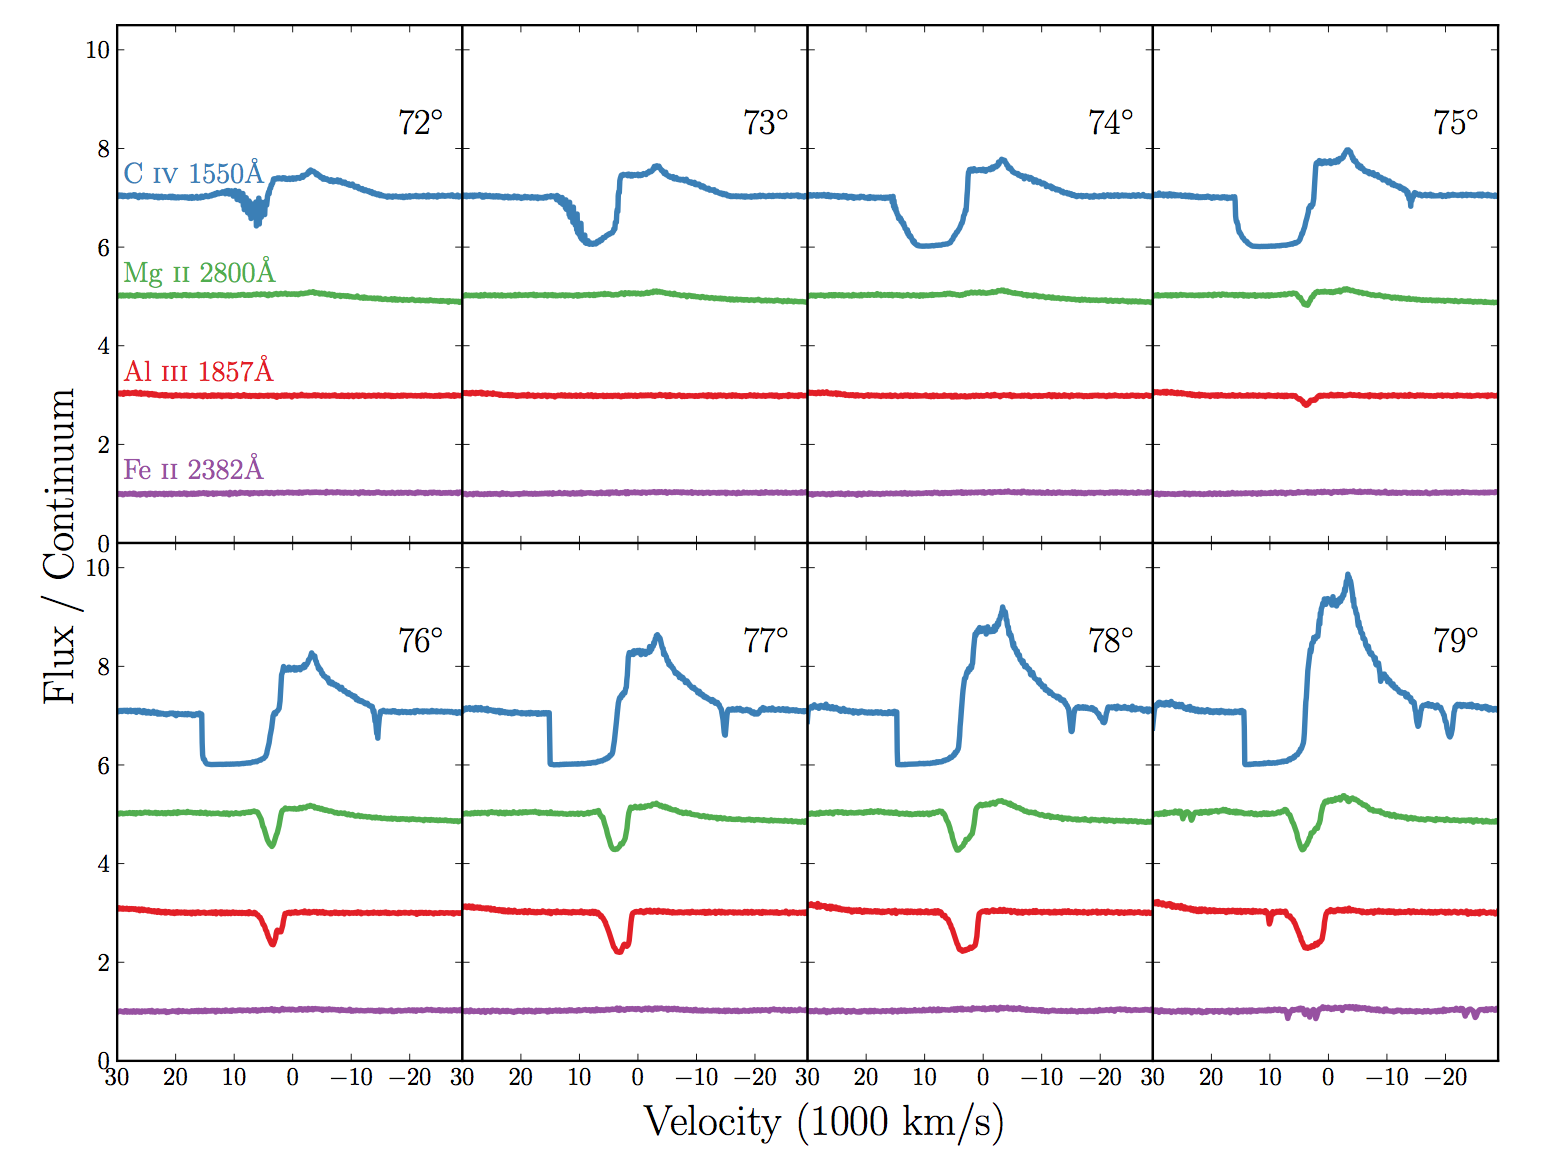
\includegraphics[width=1.0\textwidth]{figures/06-agnpaper/fig7.png}
\caption
[\civ , \mg , \al\ and Fe~\textsc{ii} line profiles for wind viewing angles.]
{
\civ , \mg , \al\ and Fe~\textsc{ii} line profiles for viewing angles
from $72-79^\circ$. The profiles are plotted relative to the local
continuum with an offset applied for clarity. Lower ionization
profiles appear at a subset of high inclinations, compared
to the ubiquitous \civ\ profile.
}
\label{fig:lobal}
\end{figure*}


At high inclinations, the synthetic spectra exhibit 
blue-shifted BALs in \al\ and \mg --
the absorption lines seen in LoBALQSOs -- 
and even show absorption in Fe~\textsc{ii}
at the highest inclinations. Line profiles in velocity space 
for \civ, \al\ and \mg, are shown in Fig.~\ref{fig:lobal} for a range
of BALQSO viewing angles. We find that ionization stratification
of the wind causes lower ionization material to have a smaller covering factor, 
as demonstrated by figures~\ref{fig:wind} and \ref{fig:lobal}.
This confirms the behaviour expected from a unification model such as Elvis (2000). 
LoBALs are only present at viewing angles close to edge-on ($i>75^\circ$),
as predicted by polarisation results \citep{brotherton1997}.
As observed in a BALQSO sample by \cite{filizak2014}, 
the model BAL troughs are wider and deeper when low ionization 
absorption features are present,
and high ionization lines have higher blue-edge velocities than the 
low ionization species.
There is also a correlation between the strength of LoBAL features
and the amount of continuum attenuation at that sightline, particularly
blueward of the Lyman edge as the low ionization base 
intersects the line-of-sight. 
A model such as this therefore predicts that LoBALQSOs and FeLoBALQSOs 
have stronger Lyman edge absorption and 
are more Compton-thick than HiBALQSOs and Type 1 quasars.
An edge-on scenario also offers a potential explanation for the rarity of LoBAL and
FeLoBAL quasars, due to a foreshortened and attenuated continuum, 
although BAL fraction inferences are fraught with complex selection 
effects \citep{goodrich1997,krolikvoit1998}.


\section{Discussion}
\label{sec:qso_discuss}

\subsection{Parameter Sensitivity}
\label{sec:param_sens}

\begin{figure*}
\centering
\includegraphics[width=0.85\textwidth]
{figures/06-agnpaper/thesis_c4_grid.png}
\caption
[Equivalent widths and BALnicities of some important lines for the quasar wind grid.]
{
The EW of the \civ~$1550$\AA\ line at $20^\circ$ plotted against a) the 
$BI$ of \civ~$1550$\AA\ at $75^\circ$, b) the EW of the \mg~$2800$\AA\ line 
at $20^\circ$ and c) the EW of \la\ at $20^\circ$. The circles correspond 
to the simulation grid for two different values of $f_V$, and the fiducial 
model is marked with an orange star. 
We also show a higher X-ray luminosity model and a higher mass loss rate
with a red star.
}
\label{fig:grid}
\end{figure*}

Having selected an individual fiducial model from the simulation grid, it is important
to briefly explore how specialised this model is, and how small parameter
changes can affect the synthetic spectra. Fig.~\ref{fig:grid}
shows the EW at a low inclination, and $BI$ at a high inclination for the simulation
grid. A few conclusions can be drawn from this plot straight away. 
First, almost all the models with 
$f_V=0.1$ are over-ionized, and 
fail to produce strong \civ\ BALs or emission lines. Second,  
it is difficult to significantly increase line emission while
keeping the luminosity and mass loss rate of the system fixed. 
We show an additional point on figure 7 corresponding to a model with an order of
magnitude higher X-ray luminosity and double the mass loss rate. As expected, 
this results in far higher line EWs, but fails to produce BALs because
the collisionally excited emission swamps the BAL profile. In addition,
this model would lie well above the expected $L_{2kev}-L_{2500}$ 
relation in figure 5. Such a high X-ray luminosity could therefore 
not be the cause of the strong line emission seen in {\em all} Type 1 quasars.

The parameter search presented here is by no means exhaustive, and
conclusions may be limited by the specific parameterisation of the outflow 
kinematics used. Nevertheless, I suggest that the angular distribution
of both the line and continuum emission is perhaps the crucial 
aspect to understand. With this in mind, obtaining reliable orientation 
indicators appears to be a crucial observational task if we are to
further our understanding of BAL outflows 
and their connection, or lack thereof, to the 
broad line region. 

\subsection{Inclination Trends: FWHM and EW}
\label{sec:ew_in_model}

EW increases with inclination in the fiducial model.
This trend means that even though significantly denser
models can match the line EWs fairly well at low inclinations, they will then
possess overly strong red wings to the BAL P-Cygni profiles at high inclinations.
The fact that the EW increase in our model are directly related to limb-darkening 
and foreshortening of the continuum. 
This appears to contradict observations, which show remarkably uniform emission
line properties in quasars and BALQSOs \citep{weymann1991,dipompeo2012b}. 

In order to quantitatively assess how emission lines change with 
inclination when blue-shifted absorption 
may affect the line profile, I define the `red wing equivalent width' ($W_{\lambda,RW}$) as
\begin{equation}
W_{\lambda,RW} = \int_{\lambda_0}^{\lambda^\prime} \left( 1 - \frac{F_\lambda}{F_0} \right) d\lambda
\label{rwew}
\end{equation}
where $F_0$ is the continuum flux and the integral is calculated from $\lambda_0$, line centre,
to a wavelength $\lambda^\prime$ where the flux has returned to the continuum level.
This quantity is shown as a function of inclination in Fig.~\ref{fig:ew_in_model} for the \civ\ UV line.
We also plot show the $W_{\lambda,RW}$ expected from isotropic line emission and a foreshortened 
and limb darkened disc as well as $1/2$ equivalent widths from \cite{dipompeo2012b}. 

\begin{figure*}
\centering
\includegraphics[width=0.8\textwidth]{figures/06-agnpaper/ew.png}
\caption
[$W_{\lambda,RW}$ as a function of inclination in the fiducial model.]
{
$W_{\lambda,RW}$ as a function of inclination in the fiducial model, compared
to 1/2 EW from the quasar sample of Di Pompeo et al. (2012; D12).
}
\label{fig:ew_in_model}
\end{figure*}

The variation of EW with inclination is significantly 
larger than the variation across the quasar population.
The angular distribution of the disc 
continuum and line emission is clearly crucially important in 
determining the emergent broad line EWs, as suggested by, e.g., 
the analysis of \cite{risaliti2011}. 
We shall explore this question further in a future study (see chapter 6).  

\subsubsection{FWHM and Black Hole Mass Estimates}

In a recent study, \cite{yong2016} used the SV93 wind prescription
assess the variation of full-width at half-maximum (FWHM) of 
\hb\ (and resultant BH mass estimates)
with inclination in a disc wind model. Although their model is fairly simple -- 
it does not include, for example, full radiative transfer or ionization physics --
this analysis still gives interesting insights into how emission lines
from a disc wind might bias BH mass estimates.

If the BLR gas is virialised, as often assumed, then the black hole mass
is related to the velocity dispersion, $\Delta v$, of the gas by
\begin{equation}
M_{BH} = f \frac{\Delta v^2 R_{BLR}}{G},
\end{equation}
where $R_{BLR}$ is some appropriate emissivity-weighted radius and is often 
either assumed, estimated from ionization arguments or calculated from reverberation
mapping. When using FWHM to estimate the velocity disperson the above
equation can be rewritten as
\begin{equation}
M_{BH} = f_{FWHM}~\left[c~\frac{(FWHM)}{\lambda_0}\right]^2~\frac{R_{BLR}}{G},
\end{equation}
where $\lambda_0$ is the central wavelength of the line in question
and the FWHM is in the same wavelength units.
In a model such as ours the BH mass is known, and determines
the escape velocities and rotational motions of the outflow. Thus, 
using a typical radius for line formation in the model it is trivial to 
calculate $f_{FWHM}$ for each viewing angle. Fig.~\ref{fig:FWHM}
shows $f_{FWHM}$ as a function of inclination for the 
\civ, \mg\ and \ha\ emission lines in our model, 
assuming $R_{BLR}=10^{17}$~cm. 
For \civ\ and \mg\ the wind angles are not plotted as BAL profiles affect 
the measurement, and I have compared to \ha\ rather than \hb\ due to the
low \hb\ luminosity at some viewing angles. We nevertheless
expect this value to trace $f_{FWHM}$ from \hb\ fairly well.

The values from our model agree fairly well with the predictions
of \cite{yong2016} from their simpler analysis, suggesting that,
at least in this specific set-up,
radiative transfer and ionization has a minimal role in determining
the emergent FWHM. Instead, the effect is dominated by velocity projection
effects. The reason for the significantly lower values for \mgii\ is that
it is actually formed well inside $R_{BLR}=10^{17}$~cm, highlighting
the dangers of using a single BLR radius for BH mass estimates
from different lines.

\begin{figure}
\centering
\includegraphics[width=1.0\textwidth]{figures/06-agnpaper/f_factor.png}
\caption
[$f_{FWHM}$ as a function of inclination]
{
$f_{FWHM}$ as a function of inclination from the fiducial model
for three different lines, compared to values from
Yong et al. 2016 and Pancoast et al. 2014. 
}
\label{fig:FWHM}
\end{figure}

%%%%%%%%%%%%%%%%%%%%%%%%%%%%%%%%%%%%%%%%%%%%%%%%%

% SUMMARY

%%%%%%%%%%%%%%%%%%%%%%%%%%%%%%%%%%%%%%%%%%%%%%%%%

\section{Summary And Conclusions}
\label{sec:qso_conclusions}
We have carried out MCRT simulations using a simple
prescription for a biconical disc wind, with
the aim of expanding on the work of H13. To do this, two main
improvements were necessary: First, I included a simple treatment of 
clumping, and second, 
the modelling of recombination lines was improved by treating H and He as
`macro-atoms'. 
Having selected a fiducial model from an initial simulation grid,
I assessed the viability of such a model for geometric 
unification of quasars, and found the following main points:
\begin{enumerate}
\item Clumping moderates the ionization state
sufficiently to allow for the 
formation of strong UV BALs while agreeing well with the X-ray
properties of luminous AGN and quasars. 
\smallskip
\item A clumpy outflow model naturally 
reproduces the range of ionization states
expected in quasars, due to its stratified density
and temperature structure. 
LoBAL line profiles are seen at a subset of viewing angles, and Fe~\textsc{ii}
absorption is seen at particularly high inclinations. 
\smallskip
\item The synthetic spectra show \la\ line and weak He~\textsc{ii}~$1640$\AA\ line
as a result of our improved treatment of recombination using macro-atoms. We also see
Balmer emission lines and a Balmer recombination continuum in the optical spectrum, but this
is only really significant at high inclination where to continuum is suppressed.  
\smallskip
\item The higher X-ray luminosity causes a significant 
increase in the strength of the collisionally excited emission
lines produced by the model. 
However, the equivalent-width ratios of the emission lines do not match
observations, suggesting that a greater volume of dense ($n_e\sim10^{10}$~cm$^{-3}$)
material may be required.
\smallskip
\item The line EWs in the synthetic spectra increase with inclination.
BAL and non-BAL quasar composites have comparable EWs, so our model
fails to reproduce this behaviour.
 If the BLR emits fairly isotropically then for a 
foreshortened, limb-darkened accretion disc 
it is not possible to achieve line ratios at low inclinations 
that are comparable to those at high inclinations. 
We suggest that understanding the angular distribution of 
line and continuum emission is a crucial question for theoretical models.
% Furthermore, this is conclusion is independent of the assumed 
% BLR geometry and size.
\end{enumerate}
Our work confirms a number of expected outcomes from a geometric unification 
model, and suggests that a simple biconical geometry such as this can come close to 
explaining much of the  phenomenology of quasars. However, our conclusions pose 
some challenges to a picture in which BALQSOs are
explained by an {\em equatorial} wind rising from a classical thin disc, and suggest 
the angular distribution of emission is important to understand if this 
geometry is to be refuted or confirmed. We suggest that obtaining reliable 
observational orientation indicators and 
exploring a wider parameter space of outflow geometries in simulations
are obvious avenues for future work. % Experiment 2

\newpage
\lhead{\emph{6. Orientation Effects and Equivalent Width Distributions in Quasars}}
\chapter{Quasar Emission Line Equivalent Widths as Probes of Orientation and Unification}

%% Codes
\def\py{\textsc{python}}
\def\tar{\textsc{tardis}}
\def\cld{\textsc{cloudy}}
\def\agn{\textsc{agnspec}}
\def\kerrtrans{\textsc{kerrtrans}}


%% Lines and ions
\def\civ{C~\textsc{iv}}
\def\nv{N~\textsc{v}}
\def\heii{He~\textsc{ii}}
\def\ovi{O~\textsc{vi}}
\def\la{Ly$\alpha$}
\def\ha{H$\alpha$}
\def\ept{$\epsilon(\theta)$}

%% Journal definitions
\def\araa{ARAA}
\def\nat{Nature}
\def\apjl{ApJ Letters}
\def\aapr{AAPR}
\def\ssr{SSR}
\def\apj{ApJ}
\def\apjs{ApJs}
\def\pasp{PASP}
\def\aap{A\&A}
\def\mnras{MNRAS}
\def\aj{AJ}
\def\rmxaa{RMXAA}
\def\ew{{\rm EW}}


%%%%%%%%%%%%%%%%%%%%%%%%%%%%%%%%%%%%%%
%
%          ABSTRACT
%
%%%%%%%%%%%%%%%%%%%%%%%%%%%%%%%%%%%%%%%
\maketitle

% {\bf{\sl{\huge Abstract}}}

% The incidence of broad absorption lines (BALs) in quasar samples is 
% often explained by a geometric unification model consisting
% of an accretion disc and an associated outflow.
% This outflows is assumed to have a covering factor roughly equivalent to
% the BAL fraction, $f_{BAL}$. We test this model
% by examining ultraviolet (UV) emission line equivalent-widths. 
% We find that a model in which the 
% continuum emission arises from a geometrically thin, 
% optically thick accretion disc is inconsistent with this property
% unless (i) the line emission has the same angular distribution of 
% emission as the continuum or (ii) BAL quasars are viewed from a low or intermediate inclination. 
% We examine whether an accretion disc can emit isotropically, and
% demonstrate that general relativistic effects cannot sufficiently isotropise the 
% radiation field in the UV. 
% We suggest that reprocessing by outflows, or limb brightening due to X-ray irradiation, may play a role.
% We then explore in what limits line emission can emit with the same angular
% distribution as a foreshortened, limb-darkened disc, and discuss our results
% in the context of other observational studies of broad emission line 
% equivalent-widths in quasars.
% Finally we explore geometries in which BAL quasars are viewed
% from a low or intermediate inclination with reference to polarisation
% and modelling results. We also discuss the effect of the outflow 
% geometry on the inferred BAL fraction. We favour a scenario in which the 
% BAL outflow is {\em not} equatorial, and BAL quasars
% are instead viewed from $\sim45^\circ$ as suggested from radio measurements,
% but a number of open questions remain.

% \clearpage

%%%%%%%%%%%%%%%%%%%%%%%%%%%%%%%%%%%%%%
%
%          INTRODUCTION
%
%%%%%%%%%%%%%%%%%%%%%%%%%%%%%%%%%%%%%%%

{\em This chapter is based on a paper in preparation of the same title, 
due to be submitted to MNRAS.}

\section{Introduction}
% {\color{blue}
% Introduction to the topic, particular relating to unification
% and BAL geometries. At the moment this is a placeholder.
% }
% \bigskip

%\noindent
% A number of quasar unification schemes have attempted to explain 
% the incidence of BAL quasars in terms of an outflow which rises 
% from an accretion disc \citep[e.g.][]{MCGV95, elvis2000}. 
% The covering factor of this outflow is then
% expected to determine the BAL fraction, $f_{BAL}$, thought to be
% between $20\%$ and $40\%$ 
% \citep{weymann1991, reichard2003, knigge2008, allen2011}.
% These outflows are of wide-reaching astrophysical significance as 
% they may be an efficient way for the central accretion engine to interact
% with its galactic environment (REFs), potentially explaining 
% for the $M-\sigma$ relation (REFs).

% Unlike in galactic accretion disc systems, measuring inclinations
% for quasars and AGN is notoriously difficult, and obtaining 
% reliable orientation indicators is thus an important observational
% goal for the community. Directly opposing 
% geometries have been proposed for BAL outflows, mostly from observations
% of radio-loud sources. A number of polarisation
% studies of BALQSOs have measured large angle differences 
% from the radio jet, implying an equatorial viewing angle 
% \citep{goodrich1995, cohen1995,brotherton2006}.
% Conversely, Punsly (1991) suggests a polar geometry.
% This is supported by very high brightness temperatures 
% in some RL BALQSOs \citep{zhou2006} 
% and the fact that RL BALQSOs possess similar radio spectral 
% indices to normal RL quasars \citep{bruni2012}.  
% In addition, \cite{marin2013} find a bending angle of $\sim45^\circ$ is required to 
% explain the polarisation dichotomy of type 1 and 2 AGN using an Elvis-type wind 
% model (Elvis 2000) --  a conclusion which is potentially extendable to BAL quasars.

% BALQSOs and quasars generally possess remarkably similar emission line properties 
% \citep[e.g.][]{weymann1991,reichard2003}. This, along with Occam's razor (see figure 1),
% is one of the reasons why they are thought to be drawn from the same population 
% as non-BAL quasars. In this paper, we start by verifying the uniformity 
% of emission line properties
% between BAL and non-BAL quasars. We then derive relationships for
% the expected angular distribution of emission for accretion discs 
% (section~\ref{disc}) and emission lines (section~\ref{lines}). Finally, we discuss
% these results in the context of unification models and offer 
% a number of possible scenarios.

In the previous chapters we have explored quasar unification schemes
in which the incidence of BAL quasars is explained in terms of an outflow which rises 
from an accretion disc \citep[e.g.][]{MCGV95, elvis2000}. In chapter 5,
we found that a biconical wind model can reproduce much of the qualitative 
behaviour expected from a unified model, with some shortcomings. 
In particular, we found an angular dependence of emission-line equivalent 
width (EW), such that the EWs were much stronger at high inclination.
Here, we attack the problem from a different angle (but informed by the 
previous study), by examining UV and optical emission lines from the Sloan Digital Sky 
Survey and the potential effects of orientation on their EW distributions.

Unlike in galactic accretion disc systems, measuring inclinations
for quasars and AGN is notoriously difficult, and obtaining 
reliable orientation indicators is thus an important observational
goal for the community. Directly opposing 
geometries have been proposed for BAL outflows, mostly from observations
of radio-loud sources. A number of polarisation
studies of BALQSOs have measured large angle differences 
from the radio jet, implying an equatorial viewing angle 
\citep{goodrich1995, cohen1995,brotherton2006}.
Conversely, Punsly (1991) suggests a polar geometry.
This is supported by very high brightness temperatures 
in some RL BALQSOs \citep{zhou2006} 
and the fact that RL BALQSOs possess similar radio spectral 
indices to normal RL quasars \citep{bruni2012}.  
In addition, \cite{marin2013} find a bending angle of $\sim45^\circ$ is required to 
explain the polarisation dichotomy of type 1 and 2 AGN using an \cite{elvis2000} wind 
model --  a conclusion which is potentially extendable to BAL quasars.



\section{Data Sample}
% {\color{blue}
% First we need to show that emission line properties of 
% quasars and BAL quasars really are similar. Do that with histograms 
% of EWs. We will probably show a mixture of emission lines so we cover
% allowed dipole, forbidden and intercombination lines. 

% Questions:

% \begin{itemize}
% 	\item Do we need some kind of test statistic here? e.g. K-S
% 	\item Perhaps we should derive theoretical quasar distribution with different 
% 		  inclination cutoffs?
%     \item Do we want to repeat the analysis of Risaliti et al? 
%     \item It may make sense to start with theory, derive model distributions and 
%     	  then test them against real distributions for different physical models
%     	  and inclination cutoffs?
% \end{itemize}
% }
\begin{figure*} %fullpage
\centering
\includegraphics[width=1.0\textwidth]{figures/ewpaper/composites.png}
\caption
{
SDSS Composite spectra
}
\label{fig:composite}
\end{figure*} %fullpage
% The Sloan Digital Sky Survey DR7 contains ~10,000 objects in its quasar
% catalog. Many of these have been fitted with quasar templates, allowing 
% easy comparison of the equivalent width properties between the BAL and 
% non-BAL subsamples. Figure 2 shows histograms of a number of different 
% emission line properties. As found by previous authors, we find that BAL
% and non-BAL quasars really do seem to possess very similar emission line 
% properties.

% \begin{table}
% \begin{tabular}{p{2cm}p{1cm}p{1cm}p{1cm}p{1cm}}
% Sample & Redshift Range & Number of non-BAL Objects & Number of BAL objects & Number of LoBAL objects \\
% \hline \hline 
% A & $?<z<?$ & 
% \hline 
% \end{tabular}
% \caption{
% The properties of our subsamples, built from the SDSS DR7
% quasar catalog.
% }
% \label{tab:samples}
% \end{table}

\begin{figure*} %fullpage
\centering
\includegraphics[width=1.0\textwidth]{figures/ewpaper/bals_scatter.png}
\caption
{
BH mass and Eddington fraction for the BAL samples plotted 
over the overall quasar sample from S10.
}
\label{fig:bal_scatter}
\end{figure*} %fullpage



\begin{figure*} %fullpage
\centering
\includegraphics[width=1.0\textwidth]{figures/ewpaper/ew_hist_qsos.png}
\caption
{
Histograms of equivalent widths for three emission lines from the two different samples.
}
\label{fig:ew_hists}
\end{figure*} %fullpage

To construct our sample, we start with the the Shen et al. (2010; hereafter S10) catalog of
105,783 quasars from the The Sloan Digital Sky Survey (SDSS) DR7. 
As we will use emission line diagnostics in this study, we must further divide
this sample  according to which emission lines are present in 
the SDSS wavelength range at a given redshift. 
Sample A contains all quasars within the redshift range $0.35<z<0.83$, 
such that the Mg II 2800A and OIII 5007A line EWs are both measured, and Mg II BAL identification
is possible.  Sample B contains all quasars within the redshift range $1.45<z<2.28$, such that 
the EWs and presence of BALs in Mg II 2800A and CIV 1550A are both measurable.
The details of these samples are shown in table 1.

In attempting to draw broad conclusions about unification models as a whole,
we would like to be able to construct a large homogenous dataset of 
{\em HiBAL} and non-BAL quasars with both OIII 5007A EWs. Unfortunately,
the wavelength limits of SDSS do not allow this. One of the problems with
using just LoBAL quasars as tests of unification is that there is evidence 
that they are drawn from a different population than normal quasars, perhaps
suggesting an {\em evolutionary} origin. Examples include anomalously 
high LoBAL fractions in dust-reddened quasar samples \citep{urrutia2009} 
and infra-red selected samples \citep{dai2012}; although see also \cite{lazarova2012}.
To partially address this issue, we also build a small sample of HiBAL quasars in SDSS
by cross-matching the S10 catalog with BALs identified in the HST COS archive.
BALs were selected from the COS spectra using the balnicity index (Weymann et al. 1991), 
$BI$, defined as
\begin{equation}
BI = \int^{25000~{\rm km~s}^{-1}}_{3000~{\rm km~s}^{-1}} C \left( 1 - \frac{f(v)}{0.9} \right) dv.
\end{equation}
The constant $C=0$ everywhere, unless the normalized flux
has satisfied $f(v)<0.9$ continuously for at least $2000$~km~s$^{−1}$, 
whereby $C$ is set to $1$. HST objects were designated as HiBALS 
by satisfying the condition that $BI>0$ in one of CIV, NV, SiIV.
The mass and Eddington fraction measurements from S10, with errorbars, are shown against
the background distribution of all quasars.

Figure 2 shows histograms of a number of different 
emission line properties for samples A and B. 
As discussed by previous authors \cite[e.g.][]{weymann1991}, we find that BAL
and non-BAL quasars really do seem to possess very similar emission line 
properties. The EW is related to the `face-on' equivalent width,
$EW_0$ by the equation
\begin{equation}
\ew = \ew_0 /~\epsilon(\theta)
\end{equation}
where $\theta$ is the viewing angle with respect to the symmetry axis 
and $\epsilon(\theta)$ is the `angular emissivity function', which describes 
how the continuum luminosity from the disc varies as a function of viewing angle.
For a foreshortened disc this is simply $\epsilon(\theta) = \cos \theta$.

Thus, if BAL quasars are viewed from a larger viewing angle on average then one
would expect them to possess higher EWs, with a broader distribution.
It is already apparent from figure 1 that the BAL distribution mean 
is not systematically higher than the non-BAL
mean -- in fact, it is lower. This is not expected from a model
in which the continuum is foreshortened and BAL outflows are at all equatorial.
This problem is examined further in section~\ref{sec:mc_angular}. 
First, we will examine the motivations for different forms of \ept\ 
in AGN and quasars.

\section{The Angular Distribution of Emission from an Accretion Disc and Broad-Line Region}
\label{disc}

\noindent 
The most widely-used theoretical model for an accretion disc
was proposed by Shakura \& Sunyaev (1973; hereafter SS73). 
\nocite{shakurasunyaev1973}
There are a number of well-documented problems when fitting 
AGN SEDs with SS73 accretion disc models (REFs), and there are also 
tensions with the `accretion disc size' relation from time lags \citep{edelson2015}
and microlensing \citep{morgan2010}. Despite these problems, 
\cite{capellupo2015} recently had 
some success fitting VLT XSHOOTER spectra of AGN when the effects of
GR, mass-loss and comptonisation were included.
In this section, we start by discussing the angular distribution of
emission from an SS73 disc, before discussing opacity and GR 
effects. In order to explore these effects, we use \agn\
\citep{hubeny2000,davishubeny2006,davis2007}. We stress that the 
discussion here is not limited to SS73 discs; the only real condition
for the expected angular distributions derived here is that the 
disc is geometrically thin and optically thick.

\subsection{Standard Thin Disc Models}

\noindent
A geometrically thin, optically thick disc will appear
foreshortened and limb darkened (if temperature decreases
with height from the central disc plane). 
Foreshortening is a simple $\cos \theta$ geometric effect, 
where $\theta$ is the inclination with respect to the vertical z axis, which
is perpendicular to the disc plane.
Limb darkening, $\eta(\theta)$, is given by
\begin{equation}
\eta(\theta) = a \left( 1 + b \cos \theta \right),
\end{equation}
where $a$ is a normalisation constant and $b$ governs the strength
of the limb darkening. $b=3/2$, known as the Eddington approximation
tends to given good agreement with solar observations 
\citep[e.g.][]{mihalas}. The two effects can be 
combined to give an angular emissivity function, of
\begin{equation}
\epsilon(\theta) = a \cos \theta \left( 1 + \frac{3}{2} \cos \theta \right).
\end{equation}

\subsection{Including GR, Comptonisation and Opacity Effects}

\noindent
In reality, limb darkening is not frequency independent and 
depends on the bound-free and bound-bound opacities in the disc.
In addition, it has been shown that GR can `isotropize' the radiation
field in XRBs \citep{zhang1997,munozdarias2013}, in some cases overcoming
foreshortening effects. To assess the impact of GR and disc opacities
on \ept\ we use \agn\ models, which uses stellar atmosphere calculations to calculate the 
SED in a series of annuli, before using the \kerrtrans\ code 
to calculate the emergent SED by ray-tracing along Kerr geodesics.
In Fig.~\ref{fig:agnspec_disc}, we show \ept\ as a function of 
$\theta$ for \agn\ models for minimally and maximally spinning BHs,
compared to foreshortened and limb-darkened predictions for SS73 models.
Clearly, there is very little effect; 
the accretion disc is still strongly anisotropic in the relevant wavebands.

\begin{figure}
\centering
\includegraphics[width=1.0\textwidth]{figures/ewpaper/agnspec.png}
\caption
{
Monochromatic continuum luminosities from AGNSPEC and classical thin disc
models.
}
\label{fig:agnspec_disc}
\end{figure} 
% Including GR, Comptonisation and Opacity Effects

\subsection{Alternative Continuum Models: Irradiation and Truncated Discs}

Alternative Models exist...






\section{Predicted EW distributions compared to observations: A Monte Carlo approach}
\label{sec:mc_angular}

\begin{figure}
\centering
\includegraphics[width=1.0\textwidth]{figures/ewpaper/fig2_cartoon.png}
\caption
{
The geometry of the toy model used to carry out the Monte Carlo simulations
}
\label{fig:cartoon}
\end{figure}


We assume
$\epsilon(\theta) = \cos \theta$, as this is the conservative estimate. 
% Unfortunately, it is very difficult to construct an intrinsic `face-on' distribution
% of EWs in quasars. This is mainly because the intrinsic face-on luminosities
% and inclination distribution of the systems is not known, meaning that deconvolving
% these effects is challenging. If an intrinsic, face-on distribution could be constructed
% then models of continuum emission could be used to derive predicted EW distributions
% for a grid of outflow geometries. These predicted distributions could then be compared 
% to the observed distributions and constraints placed on BAL viewing angles via,
% e.g., a Kologomorov-Smirnov test. Despite these difficulties, it is still relatively easy to 
% demonstrate that the EW distribution
% in BAL quasars is not well produced by a model in which the accretion disc is foreshortened 
% and BAL quasars are viewed from high inclinations. We will show this by first qualitatively
% examining the effect of inclination on a log-normal distribution of EWs, before conducting
% a simple Monte Carlo experiment to ascertain which geometries best reproduce the observed
% distributions.

% \subsection{The Effect of Inclination on a Log-normal EW distribution}

% Fig.~\ref{fig:ew_cartoon} shows the effect of different viewing angles 
% for BAL and non-BAL quasars for four different geometries. In each case, the
% intrinsic EW distribution, $g({\rm EW})$ is taken to be a normal
% distribution with $\mu=10$\AA and $\sigma=5\AA$. 
% We then choose $10^6$ isotropic angles on the sky and apply a 
% flux selection effect, and designate each of the angles that passes the selection 
% criteria as a BAL or non-BAL viewing angle. We assume
% $\epsilon(\theta) = \cos \theta$, as this is the conservative estimate. 
% Viewing BALs from high inclinations results in both a systematic shift in the mean to
% higher EWs, as well as a broader distribution, with the characteristic tail at 
% extreme inclinations. 

% \begin{figure*} %fullpage
% \centering
% \includegraphics[width=1.0\textwidth]{figures/ewpaper/ew_with_cartoon.png}
% \caption
% {
% Histograms of equivalent widths for BAL and non-BAL quasars for a number of
% different toy unification geometries.
% }
% \label{fig:ew_cartoon}
% \end{figure*} %fullpage

% \subsection{Monte Carlo Approach}

\begin{figure*} %fullpage
\centering
\includegraphics[height=1.0\textwidth, angle=90,origin=c]{figures/ewpaper/contour_ew_o3.png}
\caption
{
Contour plots from the Monte Carlo simulations.
}
\label{fig:contour}
\end{figure*} %fullpage

Our Monte Carlo simulation undergoes the following steps:

\begin{enumerate}
	\setlength\itemsep{1em}
	\item A set of isotropic angles is chosen such that $P(\theta)\propto d\Omega(\theta)$.
	If $\theta_{min}<\theta<\theta_{max}$ then the fake object is flagged as a mock BAL. 
	If $\theta<\theta_{min}$ then the fake object is designated a non-BAL, and otherwise
	the object is ignored. To be included in the sample, the object also has to 
	survive a selection test based on a arbritrary flux selection limit, to simulate the
	distribution of angles in a flux-limited sample.
	\item We then construct our best estimate of the intrinsic (i.e. `face-on')
	EW distribution for non-BAL quasars. This is done via a $\chi^2$ minimisation,
	by finding the gaussian with $\mu$ and $\sigma$ which best 
	reproduces the observed distribution when convolved with
	the non-BAL angles generated in the previous step. 
	a $\chi^2$ minimisation.
	\item For each mock sample, a EW$_0$ is drawn from the intrinsic gaussian.
	\item a mock EW is estimated such that $\ew = EW_0 / \epsilon(\theta)$,
	and this process is repeated to build up a mock sample of objects.
	\item The number of objects in the mock sample with 
	$\theta_{min}<\theta<\theta_{max}$ is recorded, providing an 
	estimate of the expected BAL fraction for this wind geometry. 
	This already includes a selection effect for the weaker continuum flux.
	\item The value of the K-S test statistic is recorded, in which the 
	mock BAL sample is compared to the real BAL sample. We also record the 
	mean and variance of the mock sample. This allows us to ascertain which regions
	of parameter space best fit the observed BAL distribution
\end{enumerate}

This process is repeated for a grid of $\theta_{min}$ and $\theta_{max}$. The 
results are shown in figure~\ref{fig:contour}, in which we plot the mean, standard deviation 
and $f_{BAL}$ as a function of $\theta_{min}$ and $\theta_{max}$. As expected,
we find that equatorial viewing angles are strongly disfavoured. 



% \subsection{Favoured Geometries}

% The methods above imply that we favour blah.

% \section{The Angular Distribution of Line Emission}

% {\color{blue}
% Angular distribution of line emission derivations,
% showing in what limits emission lines will have the same
% angular emissivity distribution as an accretion disc.
% }

% \bigskip

% \label{lines}
% Here we consider three geometries for BLR emission regions. The first is
% a spherical, cloud-like structure with no velocity gradients. 
% The second is a disc structure with Keplerian velocity components, 
% potentially with the addition of outflowing material. the third is a 
% disc-like geometry with turbulent velocity gradients.

% Optically thin line emission is always isotropic in the rest frame
% of the emitting plasma. Optically thick line emission will have an angular
% emissivity function that varies according to the geometry of the 
% emitting region and the velocity gradients present. 
% We can thus use Sobolev
% theory to derive the angular emissivity function for
% line emission. Invoking the Sobolev approximation, we can write the 
% optical depth in a non-monotonic velocity field as

% \begin{equation}
% \tau = \frac{\kappa~\rho~\sigma}{| \mathbf{\hat{n} \cdot \Lambda \cdot \hat{n} |}}
% \end{equation}

% And following \cite{MCGV95} we can derive an expression for $Q=|\mathbf{\hat{n}\cdot\Lambda \cdot\hat{n}}|$

% \begin{equation}
% Q = x
% \end{equation}


% Following \cite{hornemarsh1986} and \cite{horne1995}, we can write the line optical depth as
% \begin{equation}
% \tau_\nu = \tau_0 \exp \left[ - \frac{1}{2} 
% \left( \frac{V - V_0}{\Delta V} \right)^2 \right],
% \end{equation}
% where $\tau_0$ is the line centre optical depth given by
% \begin{equation}
% \tau_0 = \frac{W}{}
% \end{equation}


\section{Discussion}

We have demonstrated that the EW distributions of the OIII emission line
in quasars is not consistent with a model in which BALs are 
viewed from equatorial angles and the continuum emission originates from
a foreshortened accretion disc. This conclusion would be strengthened were 
we to include limb darkening. This conclusion is extendible to the broad 
emission lines (IS IT?), with the caveat that those lines are dipole 
transitions and so opacity effects can change the angular distribution of emission.
A number of other observations...



\subsection{Radio Observations}

Figure~? shows the equivalent width distributions in radio-loud quasars, 
split into core or lobe dominated. This designation is commonly used
as an orientation indicator \citep{orr1982,wills1995}. 
Although th


In this case, we can
see that 
A full investigation of this is beyond the scope 

% {\color{blue}
% Alternative geometries and polarisation. Are there any problems with
% a more moderate viewing angle for BALs? Do we want to show a cartoon?
% Discuss modelling work. Also discuss compton-thick fraction at high mass end.
% What about PHYSICS. Can we derive lower limits on outflow angles from
% e.g. conservation of angular momentum??
% }


\subsection{Polarisation}

Discuss polarisation

\begin{figure}
\centering
\includegraphics[width=1.0\textwidth]{figures/ewpaper/hist_p.png}
\caption
{
{\sl Top:} 
Polarisation percentages as a function of measured inclination from
Marin et al. (2015) for Type I and Type II AGN.
{\sl Bottom:} Histograms of polarisation percentages 
for BAL quasars from Schmidt et al. (1999) together with the 
Marin et al. (2015) AGN sample. 
}
\label{fig:lobal}
\end{figure}


\subsection{Compton-thick Fractions}

Compton-thick Fractions

\subsection{Theoretical Considerations}

Discuss Proga models: They tend to rise fairly equatorially (see eg. PK04) Talk to Nick?


\section{Conclusions}

We find four possible scenarios:

\begin{itemize}
	\item {\sl Scenario 1:} Quasar discs are much more isotropic than one might expect from an SS73 type disc.
    We have ascertained that general relativistic effects cannot account for discrepancy in the UV. Reprocessing by surrounding dense plasma with a large covering factor, or limb brightening caused by X-ray irradiation, may provide possible explanations which we do not yet confirm or refute.
    \smallskip
	\item {\sl Scenario 2:} Quasar discs are strongly anisotropic, as expected from a geometrically thin, optically thick accretion disc. In this case we expect $f_{BAL} \sim 1$ 
	due to the selection effects at work, and a velocity field yadiyada.
	\smallskip
	\item {\sl Scenario 3:} BAL outflows are more collimated than expected from early
	polarisation measurements. This easily explains the emission line properties of BAL 
	and non-BAL quasars. However, equatorial geometries have been most successful when modelling
	BAL quasars, and there are clear differences in the polarisation properties of BAL and
	non-BAL quasars. We recommend that future RT modelling efforts explore different outflow geometries and that detailed polarisation modelling is undertaken to constrain the outflow opening angles.
	\smallskip
	\item  {\sl Scenario 4:} The geometric unification model does not explain the incidence of BALs in quasar, or requires an additional component which is {\em time-dependent}, such as an evolutionary or accretion state origin for BAL outflows. In this scenario, BAL quasars would be seen from very similar angles to non-BAL quasars. However, the evidence for this is limited and there is no good model for why outflows would exist only
	for $\sim 20\%$ of a quasar's lifetime. Even if this is the case, then the covering factor of the outflow still needs to be constrained in order to estimate the BAL duty cycle.
\end{itemize}
Of these, we favour scenario 3, as RT modelling of complex geometries is often degenerate
(see Borguet et al. 2010 and Matthews et al. 2015 for details) and the differences in measured
polarisation angle to not necessarily 

 % Experiment 2

% \centering
% \includepdf[pages=-]{Chapters/agnpaper.pdf}

%\chapter{Quasar Emission Lines as Probes of Orientation and Unification}



{\em This chapter is based on the paper:

Matthews J. H., Knigge C., Long, K.S. 
`Quasar emission lines as probes of orientation: 
implications for disc wind geometries and unification',
MNRAS, DOI:10.1093/mnras/stx231.

The discussion on flux limits therein should be consulted.
}


%%%%%%%%%%%%%%%%%%%%%%%%%%%%%%%%%%%%%%
%
%          ABSTRACT
%
%%%%%%%%%%%%%%%%%%%%%%%%%%%%%%%%%%%%%%%
\maketitle

\section{Introduction}

In the previous chapter, I presented tests of geometric unification
models using MCRT and photoionization simulations. 
One of the key results from that analysis is that trends with
inclination prohibit models with equatorial outflows matching
observations, as the EWs of the broad emission lines tend
to increase with inclination in the models. 
This suggests a fundamental issue with the simplest geometric 
unification models. There must be a problem with either the prescription for the 
continuum emission or the equatorial outflow geometry; otherwise,
geometric disc wind unification models of BAL and non-BAL quasars simply 
cannot reproduce the observed spectra.

One way of constraining the outflow geometry 
is by understanding the orientations
of BALQSOs, or, equivalently, the opening angles of their winds.
The covering factor and opening angle of the outflow
are also important quantities for estimating the
feedback efficiency \citep[e.g.][]{borguet2012}, measuring
the BAL fraction \citep[e.g.][]{krolikvoit1998}
and understanding the outflow physics \citep[e.g.][]{proga2005}. 
The motivation to measure orientations is not limited to disc wind models; the
AM85 and UP95 unification schemes described in section~\ref{agn_unification}
both attempt to explain the diverse behaviour of AGN merely as a function of viewing 
angle. Orientation indicators therefore also allow us to explore if these models
adequately explain the type 1/type 2 dichotomy in AGN.

Unlike in galactic accretion disc systems, measuring inclinations
for quasars and AGN is notoriously difficult \citep[see e.g.][]{marin2016}. 
Obtaining reliable orientation indicators is thus an important observational
goal for the community \citep[see e.g.][]{marin2016}. 
Perhaps as a result of this problem, 
directly opposing geometries have been proposed for 
BAL outflows (see section~\ref{sec:balqsos}). 
Attempts to constrain the inclinations
of BALQSOs have been made previously with
different diagnostics; for example, by considering 
radio measurements \citep{zhou2006,dipompeo2012a} or
polarisation \citep{brotherton2006}.  

Of course, if they depend on inclination, emission lines may themselves\index{emission line}
provide information about viewing angle. 
This is especially true if the line is roughly isotropic, as 
the continuum is expected to be strongly anisotropic if it is emitted from a 
geometrically thin, optically thick accretion disc. 
It follows that, if we can estimate the angular distribution of line and continuum emission,
the EW of an emission line can act as an orientation indicator. Conversely, if the orientations
of quasars can be measured via an independent method, 
then the emission line EW distribution can be used to test models
for the origin of the UV and optical continuum.
The variation of EW with inclination is demonstrated neatly by the behaviour 
of emission lines in high-state CVs, where inclinations are fairly well constrained.
High-state CVs show a clear trend of increasing line EW with inclination 
\citep[][see also sections~\ref{sec:NLs} and \ref{sec:modela_spectra}]{hessman1984,patterson1984,echevarria1988,noebauer},
a trend that is attributed to foreshortening and limb darkening of the disc continuum.

The ideal emission line to use for this method would be one that is completely isotropic,
i.e. {\em optically thin}. The \oiiifull\ narrow emission line fulfils this criteria -- at least in terms of its atomic physics -- since it \index{forbidden line}\index{emission line}
is a strong, forbidden line formed in the narrow-line region (NLR) of AGN. However,\index{NLR}
the ratio of \oiiifull\ to the infra-red [O\textsc{iv}]~$28.59~\mu$m line has been shown to
vary between type 1 and type 2 AGN \citep{kraemer2011}, potentially implying a degree of anisotropy.
This is discussed further in section~\ref{sec:line_aniso}.
If the line is isotropic, then any dispersion in the distribution of \oiiifull\ EW (\ewo) 
must therefore be driven by some combination of
the intrinsic luminosity \citep{borosongreen}, 
the covering factor/geometry of the NLR \citep{baskin2005} and the 
inclination of the disc. In a recent study, \citet{risaliti2011} showed that 
the \ewo\ distribution could be well-fitted by a simple model driven purely by disc inclination.
In this chapter, I apply a similar method in order to provide a fundamental test of
BAL and non-BAL quasar unification models in which the continuum source is a geometrically
thin, optically thick accretion disc. This is motivated by the remarkably similar
emission line properties of BAL and non-BAL quasars -- a similarity that would not
be expected from the simplest models in which BALQSOs are viewed from equatorial angles.

This chapter is structured as follows. First, I describe
the data sample and selection criteria being used. I begin by
simply examining the distributions of the EW of the \oiiifull\ emission line,
\ewo, and comparing the BAL and non-BAL quasar distributions. 
In section~\ref{sec:disc_agn}, I review the angular distribution of 
continuum emission one would expect from simple $\alpha$-disc models, 
as well as exploring more advanced disc models computed
with \agn. I then use these theoretical 
angular distributions applied to a simple toy model in 
section~\ref{sec:mc_angular}, and conduct MC simulations in an attempt to fit 
the observed LoBAL and non-BAL quasar distributions of \ewo, using a similar approach to 
\cite{risaliti2011}. In section~\ref{sec:discuss_ew}, I discuss the results
in the context of radio and polarisation measurements of AGN,
and explore the location of BAL quasars in `Eigenvector 1' parameter space.
I also consider the broad emission line distribution in HiBAL quasars in more detail. 
Finally, in section~\ref{sec:ew_conclusions}, I summarise the results.


\section{Data Sample}

\begin{figure*} %fullpage
\centering
\includegraphics[width=1.0\textwidth]{figures/ewpaper/bals_2x2_scatter.png}
\caption
[BH mass and Eddington fraction measurements for samples A and B.]
{
BH mass and Eddington fraction measurements from S11 for Sample A (top)
and Sample B (bottom). The LoBALQSOs in sample A and BALQSOs in Sample B are
also plotted in each case.
}
\label{fig:bal_scatter}
\end{figure*} %fullpage

\begin{figure*} %fullpage
\centering
\includegraphics[width=1.0\textwidth]{figures/ewpaper/ew_hist_qsos.png}
\caption
[Histograms of equivalent widths for three emission lines from the two different samples.]
{
Histograms of equivalent widths for three emission lines from the two different samples.
The mean of the BAL and non-BAL quasar distributions are labeled in each case, and
the histograms are normalised.
}
\label{fig:ew_hists}
\end{figure*} %fullpage

The data sample used in this chapter is based on the\index{SDSS}
\citet[][hereafter S11]{shen2011} catalog of
105,783 quasars from the The Sloan Digital Sky Survey (SDSS) 
Data Release 7 (DR7). 
As I will use emission line diagnostics in this study,
this sample must be further divided according to which 
emission lines are present in 
the SDSS wavelength range at a given redshift. 
Sample A contains all quasars within the redshift range $0.35<z<0.83$, 
such that the \mgline\ and \oiiifull\ line EWs are both measured, 
and \mg\ LoBAL identification
is possible.  Sample B contains all quasars within the redshift 
range $1.45<z<2.28$, such that 
the EWs and presence of BAL in \mgline\ and \civline\ are both measurable.
The BH mass estimates and Eddington fractions from S11 of the two sample
are shown in Fig.~\ref{fig:bal_scatter}, together with the same quantities 
for the LoBALQSOs in sample A and BALQSOs in sample B. The BH masses
are the fiducial estimates from S11, who give a detailed discussion of 
their calibration.

S11 are careful to take into account traditional problems with quasar line fitting,
such as narrow line or Fe pseudocontinuum contamination, in their fits to 
emission line profiles and resultant EW measurements. For \mgline\
this includes careful subtraction of the Fe emission using the \cite{vestergaard2001}
templates. This subtraction is not included for \civfull,
as the Fe emission is less prominent and harder to model. This may lead to
a systematic overestimate by $\sim0.05$ dex in the \civ\ line EW. 
The \oiiifull\ line is fitted with a Gaussian. The flux ratio of this line 
with the sister component of the doublet, \oiiidoublet, is found to agree well 
with the theoretical expectation of around 3, implying a reliable subtraction of broad \hb.
In order to mask out the effects of e.g., absorption, on the \civ\ and \mg\ lines, 
S11 ignore $3\sigma$ outliers in the fit to the profile. Based on these
considerations, the S11 catalog makes for a reliable set of EW 
measurements. This is especially true when making inferences from 
multiple emission lines, as systematics inherent to individual lines 
or spectral windows are less likely to affect the analysis as a whole.
\index{emission line}\index{quasar}\index{SDSS}

In attempting to draw broad conclusions about unification models as a whole,
I would ideally also construct a large, homogeneous dataset of 
HiBAL and non-BAL quasars, both with \oiiifull\ EWs. Unfortunately,
the wavelength limits of SDSS do not allow this; only LoBAL quasars have 
both BAL and \ewo\ measurements. One of the problems with
using just LoBALQSOs in tests of unification is that there is evidence 
that they are drawn from a different population than normal quasars. 
Examples include anomalously 
high LoBAL fractions in dust-reddened quasar samples \citep{urrutia2009} 
and infra-red selected samples \citep{dai2012}; 
although see also \cite{lazarova2012}.

Fig. 2 shows histograms of a number of different 
emission line properties for samples A and B. 
As discussed by previous authors \cite[e.g.][]{weymann1991}, I find that BAL
and non-BAL quasars seem to possess very similar emission line 
properties. The EW is related to the intrinsic, `face-on' equivalent width,
$\ew_*$ by the equation
\begin{equation}
\ew = \ew_* /\epsilon(\theta)
\end{equation}
where $\theta$ is the viewing angle with respect to the symmetry axis 
and $\epsilon(\theta)$ is the `angular emissivity function', which describes 
how the continuum luminosity from the disc varies as a function of viewing angle.
For a foreshortened disc this is simply $\epsilon(\theta) = \cos \theta$. 
Note that this assumes isotropic line emission, which may not be accurate for optically thick
permitted dipole transitions; the effect of line anisotropy is discussed further 
in section~\ref{sec:line_aniso}. 

If BALQSOs are preferentially viewed from larger-than-average viewing angles,
we would expect them to possess higher EWs. 
It is already apparent from Fig.~\ref{fig:ew_hists} that the BALQSO distribution means 
are not significantly higher than the non-BAL quasar
means -- in fact, in many cases they are lower. 
This is not expected from a model
in which the continuum comes from a foreshortened disc, and BAL outflows are at all equatorial.
This problem is examined further in section~\ref{sec:mc_angular}. 
First, I will examine the motivations for different forms of \ept\ 
in AGN and quasars.
\index{BALQSOs}\index{AGN}\index{quasar}

\section{The Angular Distribution of Emission from an Accretion Disc}
\label{sec:disc_agn}

\noindent 
As introduced in chapter 1, the most widely-used theoretical model for accretion discs
is the so-called `$\alpha$-disc' model of SS73. 
There are a number of well-documented problems when fitting 
AGN SEDs with SS73 accretion disc models (see section~\ref{sec:disc_continuum}), 
Despite these problems, \cite{capellupo2015} succeeded
fitting $\alpha$-disc models to AGN specta when the effects of
GR, mass-loss and comptonisation were included.
In this section, I start by discussing the angular distribution of
emission from a classic SS73 disc, before exploring opacity and GR 
effects. In order to do so, I use \agn\
\citep{hubeny2000,davishubeny2006,davis2007}. I stress that the 
discussion here is not limited to $\alpha$-discs; the only real condition
for the angular distributions derived here is that the 
disc is geometrically thin and optically thick.

\subsection{Standard Thin Disc Models}

\noindent
Any geometrically thin, optically thick disc will appear\index{accretion disc}
\index{foreshortening}\index{limb darkening}\index{accretion disc!thin disc models}
foreshortened and limb darkened (if temperature decreases
with height from the central disc plane). 
Foreshortening is a simple $\cos \theta$ geometric effect, 
where $\theta$ is the inclination with respect to the vertical z axis, which
is perpendicular to the disc plane.
Limb darkening, $\eta(\theta)$, is usually approximated by a linear dependence
of the emergent flux on $\cos \theta$, i.e. 
\begin{equation}
\eta(\theta) = a \left( 1 + b \cos \theta \right),
\end{equation}
where $a$ is a normalisation constant, and $b$ governs the strength
of the limb darkening. Setting $b=3/2$, known as the Eddington approximation,
tends to give good agreement with solar observations 
\citep[e.g.][]{mihalas}. The two effects can be 
combined to give a net angular emissivity function of
\begin{equation}
\epsilon(\theta) = a \cos \theta \left( 1 + \frac{3}{2} \cos \theta \right).
\end{equation}

\subsection{Including GR and Opacity Effects}

\begin{figure}
\centering
\includegraphics[width=1.0\textwidth]{figures/ewpaper/agnspec.png}
\caption
[Angular variation of continuum luminosity from \agn\ and classical thin disc models.]
{
Angular variation of continuum luminosity from \agn\ and classical thin disc models.
The monochromatic continuum luminosities is divided by the monochromatic continuum luminosity
at $10^\circ$, from \agn\ and classical thin disc models, at three different wavelengths.
The models are computed for an Eddington fraction of $0.2$ and $M_{BH}=10^9~M_\odot$. 
In each panel I show both Kerr and Schwarzschild \agn\ models, and the classical models are
for both pure foreshortened discs and foreshortened and limb darkened (LD) discs.
}
\label{fig:agnspec_disc}
\end{figure} 


\noindent
In reality, limb darkening is not frequency independent and \index{general relativity}
depends on the bound-free and bound-bound opacities in the disc.
In addition, it has been shown that GR light bending can `isotropize' the radiation
field in XRBs \citep{zhang1997,munozdarias2013}, in some cases overcoming
foreshortening effects. In order to assess the impact of GR and disc opacities
on \ept, I use \agn\ models, which conducts a stellar atmosphere calculation\index{\agn}
to obtain the SED from a series of annuli, before using the \kerrtrans\ code \citep{agol1997}
to calculate the emergent SED by ray-tracing along Kerr geodesics.
Fig.~\ref{fig:agnspec_disc} shows \ept\ as a function of 
$\theta$ for two \agn\ models for minimally and maximally spinning BHs. 
The models are characterised by $M_{BH}=10^9~M_\odot$ and an Eddington fraction of $0.2$.
The angular distribution is fairly insensitive to these choices.
For comparison, I also show foreshortened and limb-darkened predictions for SS73 models.
Although the \agn\ continua are significantly more isotropic at $500$~\AA,
there is very little effect redward of around $1000$~\AA, which is the relevant
region of \ept\ for \oiiifull, \civline\ and \mgline . 
In fact, using the foreshortened estimate is the conservative (least anisotropic) prescription 
in these regimes. I will thus adopt \ept$=\cos \theta$ for the remainder of this work.










\section{Predicted EW Distributions Compared to Observations}
\label{sec:mc_angular}

\subsection{Fitting the Quasar Distribution}
\label{sec:fitting}

Before comparing the \ewo\ distributions of BAL and non-BAL quasars,\index{equivalent width}
I will first examine whether the quasar sample can be fitted by a model
in which the primary driver of \ewo\ is orientation.
\citet[][hereafter R11]{risaliti2011} analysed the \ewo\ 
distribution of 6029 quasars in SDSS DR5. They demonstrated\index{SDSS}\index{emission line}
that a foreshortened disc and isotropic \oiiifull\ line produces
a high EW tail in the EW distribution, with a characteristic 
slope of $\Gamma_{EW}=-3.5$. In order to first reproduce their
result and discuss its implications, I have 
created a sample according to their selection
criteria. The criteria are that the object in question lies in the redshift
range 0.01 to 0.8, have an absolute magnitude $M_i<-22.1$, an 
apparent magnitude $m_i<19.1$, and signal to noise per pixel of greater
than 5. Using the updated SDSS quasar sample of S11, this defines
a sample of 14,424 quasars.\index{quasar}\index{SDSS}

I carried out the following procedure to simulate
the effect of inclination on the \ewo\ distribution, and used it to fit the
observed \ewo\ distribution of quasars.
This method is similar to the method used by R11 demonstrate that the power
law tail in the distribution is expected.
\begin{enumerate}
	\setlength\itemsep{1em}
	\item An isotropic angle was chosen for the mock quasar. 
	If $\theta<\theta_{1}$ then the mock quasar was designated as unobscured, 
	and otherwise it is ignored. 
	\item In order to be included in the sample, the mock quasar also had to 
	survive a selection test. This was done by drawing a random sample from the real quasar sample, 
	and calculating a `doubly observed continuum flux', $F_O$ at $5100$~\AA\ 
	(rest frame), such that $F_O = F_{5100}~\epsilon(\theta)$. The flux limit
	is set at $1\times10^{-13}$~erg~s$^{-1}$~cm$^{-1}$~\AA$^{-1}$, but the results
	are fairly insensitive to the limit chosen. This process simulates the 
	distribution of angles in a flux-limited sample under the assumption that face-on objects
	dominate the intrinsic luminosity distribution, allowing easy comparison to R11.
	\item For each mock sample, an EW$_*$ was drawn from an intrinsic 
	(i.e. `face-on') EW distribution for quasars. This was assumed to be a
	Gaussian distribution. The mean, $\mu_*$, and width, $\sigma_*$, of this Gaussian
	can either be set arbitrarily -- for example, to demonstrate trends
	in mock data -- or obtained from a $\chi^2$ fit to the observed EW
	distribution.
	\item The EW for each mock quasar 
	was estimated such that $\ew = \ew_* / \epsilon(\theta)$,
	and this process was repeated to build up a mock sample of $10^6$ objects.
\end{enumerate}
The result of this numerical experiment is, as found by R11, a distribution
with a high EW tail. I can now vary the maximum angle, $\theta_1$,
and examine how this tail changes. Mock data for a series
of maximum angles is shown in Fig.~\ref{fig:cutoff}, for two different intrinsic 
Gaussians. The power law behaviour is only seen when the maximum angle is
sufficiently large, and a rapid decay in the distribution is observed
at a characteristic EW related to both the width and mean of the
intrinsic distribution, as well as the cosine of the maximum angle.
The distribution shown in the top panel has $\mu_*$ and $\sigma_*$ from R11 Model 1, 
whereas the bottom panel shows a narrower distribution to illustrate the 
earlier onset of the high EW cutoff. 
\index{Monte Carlo}\index{equivalent width}

\begin{figure}
\centering
\includegraphics[width=1.0\textwidth]{figures/ewpaper/cutoff.png}
\caption
[Theoretical EW distributions from the numerical experiment 
described in section~\ref{sec:fitting}.]
{
Theoretical EW distributions from the numerical experiment 
described in section~\ref{sec:fitting} for a few different 
maximum angles. The results in the top panel use the same intrinsic
distribution as Model 1 from R11 (shown in black), 
whereas the bottom panel shows the distributions 
obtained from a narrower intrinsic Gaussian. By the time the maximum
angle is limited to around $70^\circ$ the cutoff is
clear even at moderate values of EW.
}
\label{fig:cutoff}
\end{figure}

Fig.~\ref{fig:chi2} shows the result of a $\chi^2$ minimization fit 
to the R11 sample. The best fit is achieved with a maximum angle of 
$\theta_{1}=83.5^\circ(^{+1.1}_{-0.5}, 3\sigma)$ and a narrower intrinsic distribution
than model 1 of R11. The run of $\Delta \chi^2$ with maximum angle
is shown in Fig.~\ref{fig:chi2_curve}, where the choice for $\mu_*$
and $\sigma_*$ is left free in each case. 
Maximum angles below $\sim80^\circ$ are strongly disfavoured
by this model. I adopt linear binning to facilitate easy comparison 
with R11, and only fit up $\ew=100$~\AA\
due to poor statistics above that limit. This 
makes inferring any information about a potential high EW cutoff 
difficult as a more complete sample at high EW is required. 

\begin{figure}
\centering
\includegraphics[width=1.0\textwidth]{figures/ewpaper/quasar_fit.png}
\caption
[The \ewo\ distribution of quasars in the R11 sample and the best fit model.]
{
The \ewo\ distribution of quasars in the R11 sample (black points), 
with $\sqrt{N}$ errorbars, and the best fit model with a maximum 
viewing angle of $84^\circ$. The intrinsic Gaussian distribution
is shown with a dashed line. The plotted data is equivalent to the non-BAL histogram 
in the top left panel of Fig.~\ref{fig:ew_hists}, except that it uses linear binning
and adopts the R11 sample criteria rather than using sample A.
}
\label{fig:chi2}
\end{figure}

\begin{figure}
\centering
\includegraphics[width=0.8\textwidth]{figures/ewpaper/chi2_o3.png}
\caption
[$\Delta \chi^2$ as a function of maximum angle.]
{
$\Delta \chi^2$ as a function of maximum angle, $\theta_1$, calculated in
steps of $0.1^\circ$. The choice for $\mu_*$ and $\sigma_*$ is 
left free in each case. The dotted line marks
the $3\sigma$ confidence interval.
}
\label{fig:chi2_curve}
\end{figure}

\subsection{Comparing non-BAL and LoBAL Distributions: Sample A}
\label{sec:bal_v_nonbal}

\begin{figure}
\centering
\includegraphics[width=0.8\textwidth]{figures/ewpaper/fig2_cartoon.png}
\caption
{
The geometry of the toy model used to carry out the Monte Carlo simulations.
}
\label{fig:cartoon}
\end{figure}

In order to compare the observed \ewo\ distributions to those expected for LoBALs and
non-BALs I conducted a Monte Carlo simulation similar to\index{Monte Carlo}
that described in section~\ref{sec:fitting}, but with a few 
key differences. I once again assumed $\epsilon(\theta) = \cos \theta$.
The geometry of the toy model used in this simulation is shown in
Fig.~\ref{fig:cartoon}. The aim is to test if this toy model can 
fit the non-BAL quasar distribution for reasonable outflow opening angles,
whilst simultaneously predicting a LoBALQSO distribution that agrees well with
the observed distributions.

First, a set of isotropic angles was generated.
If $\theta_{\mathrm{min}}<\theta<\theta_{\mathrm{max}}$, the mock quasar
was flagged as a BAL; if $\theta<\theta_{\mathrm{min}}$ it 
was designated a non-BAL, and otherwise
the object was ignored. Once again, the object also had to 
survive a selection test based on a fixed flux limit.
I then fitted the non-BAL distribution using the method described previously.
For each mock sample, a $\ew_*$ was drawn from the intrinsic gaussian,
and a mock EW was estimated such that $\ew = \ew_* / \epsilon(\theta)$.
This process was repeated to build up a mock sample of objects and 
carried out for a series of pairs of $\theta_{\mathrm{min}}$ and $\theta_{\mathrm{max}}$.
This allows theoretical distributions for BAL and non-BAL quasars
for a series of different outflow geometries to be derived.

The diagnostics recorded from the simulation are the following four
quantities:
\begin{itemize}
	\item The $p$-value associated with a two-tailed Kolgomorov-Smirnov (K-S) 
	test statistic, $p_{KS}$, in which the mock BALQSO \ewo\ distribution is compared
	to the real LoBALQSO distribution. This is not an optimized fit parameter, but rather a measure of
	the difference between the predicted BALQSO data and the observed LoBALQSO data. A small $p$-value
	is associated with a larger difference between the two distributions, as the null hypothesis that
	the two distributions are the same can be rejected at a higher confidence level.
	\item The BAL fraction, $f_{BAL}$, calculated from the 
	number of objects in the mock sample with $\theta_{\mathrm{min}}<\theta<\theta_{\mathrm{max}}$.
	This is the predicted observed BAL fraction with flux selection effects, so should be compared
	directly to the `intrinsic' values of, e.g., \cite{knigge2008} and \cite{allen2011}.
	\item The $\chi^2/dof$ from the fit to the non-BAL quasar distribution.
	\item $\Delta \mu_{EW}$, the difference between the mean value of the mock BAL
	distribution and the mean value of the mock non-BAL distribution. To mimic observations,
	this should be small.
\end{itemize}
The simulation results are shown in figure~\ref{fig:contour}, in which the 
four diagnostics are plotted as a function of $\theta_{\mathrm{min}}$ 
and $\theta_{\mathrm{max}}$. 

\begin{figure*} %fullpage
\centering
\includegraphics[width=1.0\textwidth]{figures/ewpaper/mesh4_ew_o3_max_sdss.png}
\caption
[Heat map showing the results of the MC simulation described in 
section~\ref{sec:bal_v_nonbal}.]
{
Heat map showing the results of the MC simulation described in 
section~\ref{sec:bal_v_nonbal}. The quantities shown are discussed 
further in the text, but correspond to (clockwise from top left):
the $p_{KS}$ value from a comparison between the mock BAL dataset
and the observed BAL dataset, the reduced $\chi^2$ from the fit to
the non-BAL EW distribution, the difference in mean EW between the 
mock BAL and mock non-BAL datasets, and the BAL fraction expected
for the geometry in question.
}
\label{fig:contour}
\end{figure*} %fullpage

As expected, equatorial viewing angles for LoBAL quasars 
are disfavoured, and furthermore, it is only possible to fit
the tail to the \ewo\ distribution if non-BAL quasars are allowed 
to be viewed from high inclinations. There is no region of parameter
space where a satisfactory fit is obtained to the quasar distribution
without simultaneously obtaining a large value of $\Delta \mu_{EW}$, or similarly,
a very small value of $p_{KS}$. The simulations clearly favour a geometry in which 
BALQSOs are viewed from similar angles to non-BAL quasars.

\subsection{Alternative Shapes for the Intrinsic EW Distribution}

\index{equivalent width}
The strength of the conclusions here are limited by the lack of knowledge about the 
intrinsic face-on distribution of \ewo, or, equivalently,
the orientations of the quasars themselves. 
If either of these properties were known then the results of the
K-S test and $\chi^2$ minimization could be used
to place more robust constraints on BAL and non-BAL viewing angles 
and the associated covering factor of the outflow.
% Furthermore, the distribution of \civ\ quasar EW cannot be fit by 
% the same model as the \ewo\ distribution.
Given the uncertainty about the intrinsic \ewo\ distribution, 
it is therefore important to assess how sensitive 
the various diagnostics are to its assumed Gaussian shape. 
To explore this I have repeated the MC experiment
using a Gaussian in logarithmic \ewo\ space for the intrinsic distribution, i.e.
a {\em Log-normal} distribution. The results of using this intrinsic distribution,
as opposed to a normal Gaussian, are shown in Fig.~\ref{fig:contour2}.

\begin{figure*} %fullpage
\centering
\includegraphics[width=1.0\textwidth]{figures/ewpaper/mesh4_ew_o3_max_sdds_logn.png}
\caption
[Heat map showing the results of the MC simulation described in 
section~\ref{sec:bal_v_nonbal}, but this time conducted with a Log-normal 
intrinsic distribution.]
{
Heat map showing the results of the MC simulation described in 
section~\ref{sec:bal_v_nonbal}, but this time conducted with a Log-normal 
intrinsic distribution. The quantities shown are the same 
as in Fig.~\ref{fig:contour}. Note the different scale for the colour coding
of the $\chi^2/dof$ panel (upper right).
}
\label{fig:contour2}
\end{figure*} %fullpage

There is no region of the model parameter space that produces as good a fit to
the non-BAL quasar distribution as for a Gaussian intrinsic distribution. Instead, 
the fit is much less sensitive to $\theta_{\mathrm{min}}$ and $\theta_{\mathrm{max}}$, 
resulting in $\chi^2/dof\approx3$ for virtually all model geometries. 
Unsurprisingly, there is still a substantial difference between the LoBAL and 
non-BAL quasar distribution whenever the outflow is equatorial. Clearly, one could vary the 
distribution to have almost any intrinsic shape, which could significantly
affect the fit to the non-BAL quasar distribution. In general, allowing more freedom in the 
intrinsic distribution might permit the high EW tail to be fitted at lower inclinations.
The more freedom in the intrinsic distribution, the more a hypothesis in which 
the \ewo\ distribution of quasars is not driven by viewing angle is supported.
However, importantly, the conclusions about BAL outflow geometries in the presence of
a disc-like continuum are insensitive to the assumed intrinsic distribution, because
the mean of the simulated LoBALQSO distribution will always tend to differ to the non-BAL case
by a factor roughly equal to $1/\cos \theta$, where $\theta$ is a typical viewing angle to a 
LoBALQSO.


\subsection{Caveats and Selection Effects}

It is important to be aware of selection effects that
could potentially hide any intrinsic differences in the \ewo\ distributions. 
One concern with the approach used here is that systematic differences between the
non-BAL and LoBAL quasar populations in the {\em luminosity} of the \oiiifull\ line 
and continuum could mask the expected trends in \ewo. I have verified that this is a 
small effect; although \cite{boroson1992} found weak \oiiifull\ emission in LoBALQSOs,
the distributions of $L[\mathrm{\oiii}]$ are very similar in sample A. 
The LoBALQSO sample has continuum luminosities a factor $\approx2$ higher than the
non-BAL quasar sample on average -- this is not enough to
permit high inclination models, although it does moderate the conclusions slightly.
This also shows that host galaxy contamination is not significantly different in 
the LoBALQSO sample. 

Different reddening properties in LoBALQSOs could also mask
\ewo\ trends -- however, this actually strengthens the conclusions, as
reddening is higher in LoBALQSOs than non-BAL quasars 
\citep[e.g.][]{urrutia2009}.
This would lead to either an equally obscured \oiiifull\ emission line and continuum, 
or an enhanced \ewo, depending on the geometry and covering factor of the reddening
dust. A key limitation of the method in general is the SDSS wavelength coverage,
which means that only LoBALs can be used when \ewo\ is present (sample A).
I would suggest that future observational programs might 
look to build up a large sample of \ewo\ measurements for HiBAL
quasars. 

% In the mean time, I will turn to the UV broad emission
% lines to examine if the above conclusions also hold
% when examining the properties of the HiBAL quasars in sample B.


\section{Discussion}
\label{sec:discuss_ew}
I have demonstrated that the EW distributions of the 
\oiiifull\ emission line in LoBAL and non-BAL
quasars is not consistent with a 
model in which LoBAL quasars are viewed from equatorial angles 
and the continuum emission originates from
a foreshortened accretion disc. The EW distributions of 
\civline\ suggest that a similar conclusion applies to HiBAL quasars.
This result would only be strengthened were 
I to include limb darkening. I will now explore how the above results compare to other
observations of quasars that might probe system orientation, as 
well as the potential impact of obscuration and line anisotropy
on the results.

\subsection{Eigenvector 1}

\index{Eigenvector 1}\index{emission line}\index{AGN}\index{quasar}
Eigenvector 1 (EV1) is a fundamental parameter space for AGN and quasars
\citep{borosongreen,sulentic2000ev1,marziani2001,shenho2014}. 
It relates the FWHM of \hb, the relative iron strength, 
$R_{{\rm Fe \textsc{ii}}}$, and
\ewo. Both \ewo\ and \fwh\ have been used as orientation
indicators: \fwh\ should increase with inclination if the line formation
region is at all disc-shaped due to velocity projection effects (see section~\ref{sec:model_fwhm}).
This means that comparing the LoBALQSO EV1 distribution to the non-BAL 
quasar EV1 distribution is particularly interesting. Once again,
HiBALQSOs cannot be placed on this space due to the lack of rest-frame 
optical coverage.

\begin{figure}
\centering
\includegraphics[width=1.0\textwidth]{figures/ewpaper/ev1_arrows.png}
\caption
[Eigenvector 1 for LoBAL and non-BAL quasars.]
{
Eigenvector 1 for LoBAL and non-BAL quasars. 
FWHM of the \hb\ line plotted against the relative
iron strength, $R_{{\rm Fe \textsc{ii}}}$. The colour coding
corresponds to the EW of \oiiifull. The dots mark all quasars from
sample A, while the squares mark those with \mgii\ LoBALs. 
A few of the \mgii\ LoBALQSOs are missing due to their lack of \fwh\ 
measurements. The arrows show the approximate 
direction of the expected inclination ($\theta$)
trend under both the SH14 and R11 interpretations, and the expected 
trend in Eddington fraction ($L/L_{\mathrm{Edd}}$) from SH14 only.
}
\label{fig:bal_ev1}
\end{figure}

Fig.~\ref{fig:bal_ev1} shows the quasar distribution from sample A 
in EV1 parameter space, with LoBAL quasars from sample A overplotted.
\citet[][hereafter SH14]{shenho2014} propose 
that the main inclination driver in this parameter space
is \fwh, and that high inclination sources should thus cluster nearer 
to the top of the plot. In contrast,
R11's analysis predicts that high inclination sources should cluster
around high \ewo\ widths. As \ewo\ and \fwh\ are very weakly correlated
(Spearman's rank coefficient of 0.14), this means they should lie to
the left of the parameter space, due to the clear correlation between \ewo\
and $R_{{\rm Fe \textsc{ii}}}$. These expected trends are shown with arrows
in Fig.~\ref{fig:bal_ev1}; inspection of the figure clearly 
shows that BAL quasars are not only found in one region of the 
EV1 parameter space. 

In order to assess this more quantitatively, I also show contours of 
quasar counts overlaid on the scatter plot. The contours correspond
to the number of objects in each bin, where the bins are of size
$\Delta R_{{\rm Fe \textsc{ii}}} = 0.2$ and $\Delta$\fwh$=500$km~s$^{-1}$.
The percentage of quasars falling within the inner contour is 45\%, 
whereas only 18\% of LoBALQSOs fall in the space. Conversely, 24\% 
of LoBALQSOs fall outside the outermost contour compared to 10\% of 
non-BAL quasars. It would therefore appear that BAL 
quasars are slightly preferentially clustered towards the high-mass and 
high-inclination end of EV1 space (under the interpretation of SH14).
This is further illustrated by Fig.~\ref{fig:bal_ev1_bins},
which shows the LoBAL fraction in larger bins, compared to the 
mean LoBAL fraction. This is again suggestive of an overdensity of LoBALQSOs 
towards the upper right of the parameter space.
It is also clear that a unification picture in which BAL 
quasars are viewed exclusively from high inclinations is 
inconsistent both the R11 and SH14 interpretations of EV1 parameter 
space. 

Larger datasets, preferably including HiBAL quasars with EV1 measurements, 
are needed in order to properly constrain the EV1 behaviour of BAL quasars.
However, overall, the behaviour of EV1 in LoBALQSOs slightly 
strengthens the conclusion that BAL quasars are not always viewed from 
extreme inclinations, or alternatively, that we not yet understand the real drivers
of EV1.

\begin{figure}
\centering
\includegraphics[width=1.0\textwidth]{figures/ewpaper/ev1_bins.png}
\caption
[LoBAL fraction compared to global LoBAL fraction in Eigenvector 1 space.]
{
LoBAL fraction compared to global LoBAL fraction in Eigenvector 1 space, in bins
of $\Delta R_{{\rm Fe \textsc{ii}}} = 1$ and $\Delta$\fwh$=3000$km~s$^{-1}$..
The contour shows the outermost contour from Fig.~\ref{fig:bal_ev1} for
reference. The text shows $N_{\mathrm{LoBAL}}/N_{\mathrm{non-BAL}}$, 
where $N_{\mathrm{LoBAL}}$ is the number of LoBALQSOs in the bin and 
$N_{\mathrm{non-BAL}}$ in the number of non-BAL quasars in the bin.
}
\label{fig:bal_ev1_bins}
\end{figure}

\subsection{Polarisation}

\index{polarisation}\index{disc wind}\index{absorption line}
Spectropolarimetry of BAL quasars offers some of
the best insights into the geometries of BAL outflows and 
tends to show a few key properties. The first is enhanced 
polarisation in the BAL troughs themselves \citep{schmidt1999}. 
This is readily explained by a scattering region unobscured by the
BAL trough, with the higher polarisation percentage simply due to the
decreased direct flux. This may also explain the non-black saturation in
BAL troughs (see section~\ref{sec:balqso_angles}).

The second property 
is a continuum polarisation percentage that is around $2.4$ times greater, 
on average, than seen in the non-BAL population \citep{schmidt1999}.
A histogram of the continuum polarisation percentages of a sample of BAL quasars from 
\cite{schmidt1999} are compared to the Type I and Type II AGN 
populations from \cite{marin2014} in Fig.~\ref{fig:bal_polarisation}.
The corresponding cumulative distribution function is shown in Fig.~\ref{fig:cdf_pol}.
These show that BAL polarisation percentages seem to lie between those of type 1
and type 2 AGN. If type 1 and type 2 objects are viewed from low and high 
inclinations, respectively, as expected from unified models and suggested by
\cite{marin2014,marin2016}, this would imply  an intermediate inclination
for BALQSOs. This enhanced polarisation for BALQSOs, relative to non-BAL systems,
is also well reproduced by intermediate
inclination outflows in simple radiative transfer models \citep{marin2013}.

\begin{figure}
\centering
\includegraphics[width=0.8\textwidth]{figures/ewpaper/hist_p.png}
\caption
{
Histograms of polarisation percentages 
for BAL quasars from Schmidt et al. (1999) together with the 
Marin et al. (2014) AGN sample. 
}
\label{fig:bal_polarisation}
\end{figure}

\begin{figure}
\centering
\includegraphics[width=0.8\textwidth]{figures/ewpaper/cdf_p.png}
\caption
[Cumulative distribution functions of the histograms shown in
Fig.~\ref{fig:bal_polarisation}]
{
Cumulative distribution functions of the histograms shown in
Fig.~\ref{fig:bal_polarisation} for BAL quasars from Schmidt et al. (1999) 
together with the Marin et al. (2014) AGN sample. The colour-coding and 
$x$-axis scale are the same as Fig.~\ref{fig:bal_polarisation}. 
The translucent vertical lines mark the median value in each sample.
}
\label{fig:cdf_pol}
\end{figure}

The third characteristic polarisation property of BALQSOs 
is a polarisation angle of $\gtrsim60^\circ$ with respect
to the radio jet axis in RL objects \citep[][and references therein]{brotherton2006}.
This suggests a higher inclination (compared to non-BAL quasars)
viewing angle for BALQSOs under the interpretation of a geometric model. Indeed,
early polarisation studies suggested that the observations could be explained by a model
with a polar scattering region, distinct from the BLR and BAL regions, which was 
then viewed at an equatorial angle 
\citep[e.g.][]{goodrich1995, cohen1995,lamy2004}. Regardless of
the true geometry, the reason for the difference must be understood.
I would suggest that polarisation predictions are made from wind
models such as the one I presented in chapter 5, using a similar
approach to \cite{marin2013}, but considering BALs in more detail. 
Overall, however, polarisation measurements seem to imply that BALQSOs are viewed
from higher inclinations if geometric unification models are correct and are 
in slight tension with the idea that BAL quasars are viewed from the same range
of angles as non-BAL quasars.

\subsection{The Effect of Obscuration}
\label{sec:obscure}

\index{obscuration}
\citet[][hereafter C11]{caccianiga2011} showed that the distribution of \ewo\
can also be well fitted by an obscuration model. They modelled the 
\ewo\ distribution using absorption models for 169 objects with column density
measurements from the {\sl XMM Newton} Bright Serendipitous Source (XBS)
sample. They find that AGN with column densities of 
$N_H\gtrsim10^{22}$~cm$^{-2}$ can explain the high EW powerlaw tail. 

The column density measurements for BAL quasars suggest that obscuration 
cannot explain the distribution of \ewo\ in quasars. 
As briefly discussed in chapter 5, BALs generally show
strong X-ray absorption with column densities of $N_H\gtrsim10^{23}$~cm$^{-2}$
\citep{green1996,mathur2000,green2001,grupemathur2003}. \cite{gallagher1999}
found all BAL quasars in a sample of 7 had $N_H>10^{22}$~cm$^{-2}$, placing
them firmly in the EW tail according to the C11 model. This is broadly
consistent with the mean value of $3.5\times10^{22}$~cm$^{-2}$ from
\cite{morabito2013}, and would imply that BALQSOs should have significantly
higher EWs if obscuration governs the \ewo\ distribution.
Of course, only LoBAL quasars had \ewo\ measurements 
in the sample used here -- this actually strengthens the conclusion, as low ionization 
BALQSOs show even higher column densities, approaching Compton-thick values 
\citep{morabito2011}. This argument holds regardless of the outflow geometry adopted.

I therefore suggest that the obscuration model of C11 cannot explain the \ewo\ distribution
of LoBALQSOs. The similarity of the observed LoBAL and non-BAL distributions
also means that obscuration is unlikely to drive the behaviour of \ewo\ overall.
These conclusions are moderated if the line of sight to the X-ray source, which determines 
the measured $N_H$, experiences a different absorbing column to that of the optical continuum.
They are also dependent on the particular reddening model used by C11. Indeed, it is worth noting at 
this point that there is a degree of scatter in the $N_H$ values measured from X-ray and optical
observations \citep{maiolino2001b,maiolino2001a}, as could be produced by differing 
viewing angles.
% so I suggest that the obscured model of C11 is ruled out on this basis.


\subsection{Line Anisotropy}
\label{sec:line_aniso}

\index{emission line}
Optically thin lines are isotropic -- the {\em local}
escape probabilities in each direction are equal due to the 
low optical depth. Anisotropy can however be introduced into optically thin 
line emission by variation in continuum absorption. Indeed,
\cite{kraemer2011} showed that the strength of \oiiifull\ compared
to the infra-red [O\textsc{iv}]~$28.59~\mu$m line 
varies between type 1 and type 2 AGN. This variation is due 
to frequency-dependent absorption, and should not effect the distribution of \ewo.
If a higher continuum optical depth was experienced along the line of sight
to the NLR than to the continuum source then this could hide any EW
trends. However, this is the opposite behaviour than that expected from type 1/type 2
unification geometries (see section~\ref{agn_unification}).

When lines are optically thick, the situation is more
complex, as local velocity gradients then determine the line 
anisotropy. Indeed, Keplerian velocity shear has been shown to modify the
shape of disc-formed emission lines \citep{hornemarsh1986}, and an additional
radial shear from a wind can cause double-peaked lines
to become single-peaked \citep{MC96,MC97,flohic2012}. 
Although there is a sub-population of AGN with double-peaked lines 
\citep[e.g.][]{eracleous1994,eracleous2003},
this fraction is only around $3\%$ \citep{strateva2003}, so
AGN and quasar spectra in general show broad, single-peaked lines. 

R11 suggested that the broad emission lines trace the disc
emission in terms of their anisotropy. 
If this was the case, we would not expect a difference in the BAL and non-BAL
quasar EW distributions. However, an emission line would only be purely 
foreshortened if emitted by a disc with zero velocity shear. 
The single-peaked nature of most quasar lines imply that they are not
formed in a Keplerian disc, or that radial velocity gradients modify the profile 
shapes. We can nonetheless briefly explore the expected angular distributions
expected if the lines came from a region subject to
Keplerian velocity shear. In this case, the surface brightness of an optically thick 
line is \citep{hornemarsh1986}
\begin{equation}
J_{\mathrm{thick}}(\theta) \approx \cos \theta~S_L~\Delta \nu~\sqrt{8 \ln \tau_0} \ ,
\end{equation}
where $S_L$ is the line source function (assumed constant) and
$\tau_0$ is the line centre optical depth, given by
\begin{equation}
\tau_0 = \frac{{\cal W}}{\sqrt{2}\pi \Delta \nu \cos \theta}.
\end{equation}
The parameter ${{\cal W}}$ is given by
\begin{equation}
{{\cal W}} = \frac{\pi e^2}{m_e c}f N^\prime,
\end{equation}
where $f$ is the oscillator strength and $N^\prime$ is the number
density integrated along the vertical height of the disc. The linewidth
$\Delta \nu$ is enhanced from the thermal line width by the velocity shear, such
that
\begin{equation}
\Delta \nu = \Delta \nu_{th} \left[1 + 
\left(\frac{3}{4}\frac{v_{k}}{v_{th}}\frac{H}{R}\right)^2
Q(\theta, \phi)
\right]^{1/2},
\end{equation}
where I have defined
\begin{equation}
Q(\theta, \phi) =
\sin^2 \theta \tan^2 \theta \sin^2 2 \phi.
\end{equation}
Here, $\phi$ is the azimuthal angle in the disc, $\nu_{th}$ and $v_{th}$ are the 
thermal line widths in frequency and velocity units respectively, 
$H$ is the scale height of the disc at radius $R$, and $v_k$ is the
Keplerian velocity. The outcome of the \cite{hornemarsh1986} analysis is that optically thick lines 
formed in a Keplerian disc are strongly anisotropic, but they do not follow a simple 
$\cos \theta$ distribution. Instead, the line anisotropy is
a function of the velocity shear in the disc, the atomic physics of
the line in question, the location of the line formation region 
and the vertical disc structure. 

To examine the form of this line anisotropy, 
we can now define the angular emissivity function for a line, $\epsilon_{\mathrm{line}}(\theta)$.
In the optically thick case with no additional velocity shear, 
$\epsilon_{0,\mathrm{line}}(\theta) = \cos \theta$.
In the presence of Keplerian velocity shear, and neglecting the weak $\sqrt{8 \ln \tau_0}$ term, 
we can write
\begin{equation}
\epsilon_{k, \mathrm{line}}(\theta, \phi) = \cos \theta \left[1 + 
\left(\frac{3}{4}\frac{v_{k}}{v_{th}}\frac{H}{R}\right)^2
Q(\theta, \phi)
\right]^{1/2}.
\end{equation}
This quantity is compared to $\cos \theta$ in Fig.~\ref{fig:line_aniso1} 
as a function of for a few values of $\phi$, 
using typical quasar parameters of $v_k=10,000~\mathrm{km~s^{-1}}$ and 
$v_{th}=10~\mathrm{km~s^{-1}}$, and assuming $H/R=0.01$. I also show the 
azimuthally-averaged function, $\bar{\epsilon}_{k,\mathrm{line}}$, 
which determines the integrated emergent flux as a function of $\theta$.
Fig.~\ref{fig:line_aniso2} also shows $\bar{\epsilon}_{k,\mathrm{line}}$ 
for a few different model values of $v_k, v_{th}$
and $H/R$; the models are defined in table~\ref{tab:line_mods}.

The results suggest that optically thick line emission from a\index{BLR}
disc-like BLR cannot readily explain the EW distributions of the broad emission lines,
as proposed by R11, or the similarity of the distributions of \civline\ EW and 
\mgline\ EW in BAL and non-BAL quasars. 
This is because broad emission lines formed in a Keplerian disc do not simply trace 
the disc continuum emission in terms of their angular emissivity function.
The presence of an equatorial wind would only serve to exacerbate the effect,
as it would cause more line emission to escape along the poloidal velocity gradient towards high 
inclinations. I would therefore suggest that future efforts might include fully modelling 
the line emission as a function of inclination to feed into the above analysis -- it is certainly
not sufficient to assume that a disc-shaped BLR should emit in the same way as a disc continuum.

\begin{figure}
\centering
\includegraphics[width=0.8\textwidth]{figures/ewpaper/line_azi.png}
\caption
[The line angular emissivity function from a Keplerian disc 
as a function of inclination angle.]
{
The line angular emissivity function from a Keplerian disc 
as a function of inclination angle, $\theta$, for a few different azimuthal angles, $\phi$.
The azimuthally-averaged case, $\bar{\epsilon}_{k,\mathrm{line}}$ (thick black line),
and the zero Keplerian velocity shear case, 
$\epsilon_{0,\mathrm{line}}(\theta) = \cos \theta$ (dotted line), are also shown.
}
\label{fig:line_aniso1}
\end{figure}


\begin{figure}
\centering
\includegraphics[width=0.8\textwidth]{figures/ewpaper/line_emiss.png}
\caption
[The azimuthally-averaged line angular emissivity function from a Keplerian disc 
as a function of inclination angle.]
{
The azimuthally-averaged line angular emissivity function, $\bar{\epsilon}_{k,\mathrm{line}}$,
from a Keplerian disc as a function of inclination angle for the four models shown in 
table~\ref{tab:line_mods}. The model parameters are the values of $H/R$, $v_k$ and $v_{th}$. 
The zero Keplerian velocity shear case, $\epsilon_{0,\mathrm{line}}(\theta) = \cos \theta$ (dotted line), 
is also shown. Unless the disc is very thin ($H/R\sim0.001$),
$\bar{\epsilon}_{k,\mathrm{line}}$ shows large deviations from $\cos \theta$.
}
\label{fig:line_aniso2}
\end{figure}

\begin{table}
\centering
\begin{tabular}{p{1cm}p{2cm}p{2cm}p{2cm}p{2cm}}
\hline
Model & $H/R$ & $v_k (\mathrm{km~s^{-1}})$ & $v_{th} (\mathrm{km~s^{-1}})$ \\
\hline \hline 
A & $0.01$ & $10,000$ & $10$ \\
B & $0.01$ & $5,000$ & $10$ \\
C & $0.01$ & $5,000$ & $25$ \\
D & $0.001$ & $5,000$ & $25$ \\
\hline 
\end{tabular}
\caption
[The values of the Keplerian velocity, $v_k$, thermal velocity, $v_{th}$,
and ratio of disc scale height to radius, $H/R$, for four models.]
{
The values of the Keplerian velocity, $v_k$, thermal velocity, $v_{th}$,
and ratio of disc scale height to radius, $H/R$, for four models. These values
are used as inputs to calculate $\bar{\epsilon}_{k,\mathrm{line}}$ as shown in 
Fig.~\ref{fig:line_aniso2}, and model B is also used in 
Fig.~\ref{fig:line_aniso1}.
}
\label{tab:line_mods}
\end{table}

% , and the presence of radial
% velocity shear from a wind would only complicate matters. 
% I would therefore suggest that future efforts might include fully modelling 
% the line emission as a function of inclination to feed into the above analysis.

% Regardless of the precise angular distribution, 
% line emission should not trace disc emission
% exactly, as we already know large-scale velocity fields are dynamically important
% in the BLR, purely from the line widths. In that case, one would expect systematic
% differences in EW between high inclination and low inclination sources, and these are 
% not seen in the \civline\ and \mgline\ EW distributions.

\section{Conclusions}
\label{sec:ew_conclusions}

I have explored the emission line properties of BAL and non-BAL quasars,
particularly focusing on the EW distributions in two redshift ranges of the SDSS
quasar catalog. My main conclusion is that the EW distributions of BAL and
non-BAL quasars are remarkably similar and that this is {\em not} what one would expect from
a unification model in which an equatorial BAL outflow rises from a foreshortened 
accretion disc. This geometry has been used extensively in 
geometric unification and BAL outflow models in the past 
\citep[e.g.][]{MCGV95,PSK2000,PK04,risalitielvis2010,borguet2010,
higginbottom2013, nomura2013,nomura2016} and was even adopted earlier in this thesis.
I then established that an angular emissivity function of \ept$ =\cos \theta$ 
is a fairly conservative estimate of the anisotropy expected from thin disc models, 
as GR or opacity effects in the disc do not cause the continuum to become more isotropic
in the relevant wavelength regimes. I used this form of \ept\ to conduct a series of simulations 
similar to those described by \cite{risaliti2011}.
As expected, these simulations confirmed the above finding..

There are three basic ways to explain these results (with the caveat that the conclusions
drawn about LoBALQSOs are assumed to apply to BALQSOs in general):
\begin{itemize}
	\item {\sl Scenario 1:} The quasar continuum is much more isotropic than one would
	expect from a geometrically thin, optically thick accretion disc.
    I have demonstrated that general relativistic effects cannot account for this discrepancy in the 
    UV. Reprocessing by surrounding dense plasma with a large covering factor or limb brightening 
    in the disc may provide possible explanations which this analysis cannot yet confirm or refute.
    \smallskip
	\item {\sl Scenario 2:} Quasar discs are strongly anisotropic, as expected from a 
	geometrically thin, optically thick accretion disc. In this case, BAL outflows cannot 
	only emerge at extreme inclinations and should instead be seen from fairly low inclinations. 
	Polarisation measurements need to be reconciled with this hypothesis.
	I recommend that future RT modelling efforts explore different outflow 
	geometries and that detailed polarisation modelling is undertaken to constrain the 
	outflow opening angles.
	\smallskip
	\item  {\sl Scenario 3:} The geometric unification model does not explain the incidence of 
	BALs in quasars, or requires an additional component which is {\em time-dependent}, 
	such as an evolutionary or accretion state origin for BAL outflows. In this scenario, 
	BAL quasars would be seen from very similar angles to non-BAL quasars. If this is the case,
	the covering factors and opening angles of the outflows still need to be constrained so
	that feedback efficiencies can be accurately estimated.
\end{itemize}
I have confirmed that obscuration cannot explain the EW distributions of all quasars
due to the high column density observed in BAL (and particularly LoBAL) quasars. 
Line anisotropy from a disc-shaped BLR cannot explain the observed similarities between the broad emission
line distributions if the disc is Keplerian, and it also cannot affect the 
quasar \ewo\ distributions, as \oiiifull\ is a forbidden, optically thin transition.
\index{forbidden line}

Regardless of the conclusions about BAL quasars and their outflow geometries,
this analysis allows conclusions to be drawn about the {\em overall} 
quasar population. In scenario 1, the \ewo\ distribution of quasars cannot
be driven by inclination as suggested by \citep{risaliti2011}. This would
imply that \ewo\ is a poor orientation indicator. The lack of correlation 
between \ewo\ and \fwh\ also suggests that it is not possible for them both
to be strongly orientation dependent. Even if scenario 1 holds, the \fwh\ and EV1
measurements of LoBALs imply that they are seen from similar inclinations to type 1 quasars. 
If scenario 2 holds, then this would suggest that all quasars are viewed from fairly low inclinations,
in which case the \ewo\ distribution cannot be dominated by inclination, and its shape 
must instead be governed by the intrinsic properties of the NLR.

The above three scenarios each pose a different challenge to the current
understanding of, respectively, accretion physics, outflow models
and our understanding of unification and the BAL fraction. 
This work therefore adds to the growing evidence that our simplest models are not sufficient to
describe quasars and that alternatives need to be sought.\index{accretion disc}


 % Results and Discussion

%\input{Chapters/Chapter7} % Conclusion

%% ----------------------------------------------------------------
% Now begin the Appendices, including them as separate files

\addtocontents{toc}{\vspace{2em}} % Add a gap in the Contents, for aesthetics

\appendix % Cue to tell LaTeX that the following 'chapters' are Appendices

% \chapter{An Appendix}

Lorem ipsum dolor sit amet, consectetur adipiscing elit. Vivamus at pulvinar nisi. Phasellus hendrerit, diam placerat interdum iaculis, mauris justo cursus risus, in viverra purus eros at ligula. Ut metus justo, consequat a tristique posuere, laoreet nec nibh. Etiam et scelerisque mauris. Phasellus vel massa magna. Ut non neque id tortor pharetra bibendum vitae sit amet nisi. Duis nec quam quam, sed euismod justo. Pellentesque eu tellus vitae ante tempus malesuada. Nunc accumsan, quam in congue consequat, lectus lectus dapibus erat, id aliquet urna neque at massa. Nulla facilisi. Morbi ullamcorper eleifend posuere. Donec libero leo, faucibus nec bibendum at, mattis et urna. Proin consectetur, nunc ut imperdiet lobortis, magna neque tincidunt lectus, id iaculis nisi justo id nibh. Pellentesque vel sem in erat vulputate faucibus molestie ut lorem.

Quisque tristique urna in lorem laoreet at laoreet quam congue. Donec dolor turpis, blandit non imperdiet aliquet, blandit et felis. In lorem nisi, pretium sit amet vestibulum sed, tempus et sem. Proin non ante turpis. Nulla imperdiet fringilla convallis. Vivamus vel bibendum nisl. Pellentesque justo lectus, molestie vel luctus sed, lobortis in libero. Nulla facilisi. Aliquam erat volutpat. Suspendisse vitae nunc nunc. Sed aliquet est suscipit sapien rhoncus non adipiscing nibh consequat. Aliquam metus urna, faucibus eu vulputate non, luctus eu justo.

Donec urna leo, vulputate vitae porta eu, vehicula blandit libero. Phasellus eget massa et leo condimentum mollis. Nullam molestie, justo at pellentesque vulputate, sapien velit ornare diam, nec gravida lacus augue non diam. Integer mattis lacus id libero ultrices sit amet mollis neque molestie. Integer ut leo eget mi volutpat congue. Vivamus sodales, turpis id venenatis placerat, tellus purus adipiscing magna, eu aliquam nibh dolor id nibh. Pellentesque habitant morbi tristique senectus et netus et malesuada fames ac turpis egestas. Sed cursus convallis quam nec vehicula. Sed vulputate neque eget odio fringilla ac sodales urna feugiat.

Phasellus nisi quam, volutpat non ullamcorper eget, congue fringilla leo. Cras et erat et nibh placerat commodo id ornare est. Nulla facilisi. Aenean pulvinar scelerisque eros eget interdum. Nunc pulvinar magna ut felis varius in hendrerit dolor accumsan. Nunc pellentesque magna quis magna bibendum non laoreet erat tincidunt. Nulla facilisi.

Duis eget massa sem, gravida interdum ipsum. Nulla nunc nisl, hendrerit sit amet commodo vel, varius id tellus. Lorem ipsum dolor sit amet, consectetur adipiscing elit. Nunc ac dolor est. Suspendisse ultrices tincidunt metus eget accumsan. Nullam facilisis, justo vitae convallis sollicitudin, eros augue malesuada metus, nec sagittis diam nibh ut sapien. Duis blandit lectus vitae lorem aliquam nec euismod nisi volutpat. Vestibulum ornare dictum tortor, at faucibus justo tempor non. Nulla facilisi. Cras non massa nunc, eget euismod purus. Nunc metus ipsum, euismod a consectetur vel, hendrerit nec nunc.	% Appendix Title

%\input{Appendices/AppendixB} % Appendix Title

%\input{Appendices/AppendixC} % Appendix Title

\addtocontents{toc}{\vspace{2em}}  % Add a gap in the Contents, for aesthetics
\backmatter

%% ----------------------------------------------------------------
\label{Bibliography}
\lhead{\emph{Bibliography}}  % Change the left side page header to "Bibliography"
\bibliographystyle{aabib}
%\bibliographystyle{unsrtnat}  % Use the "unsrtnat" BibTeX style for formatting the Bibliography
\bibliography{bibs/mybib.bib,bibs/stellar.bib,bibs/h14.bib,bibs/h13.bib,bibs/hamann.bib,bibs/krolik.bib,bibs/lk02.bib,bibs/agn.bib,bibs/proga_theory.bib,bibs/cv.bib}  % The references (bibliography) information are stored in the file named "Bibliography.bib"l

\end{document}  % The End
%% ----------------------------------------------------------------